\documentclass[prc,preprint,showpacs,eqsecnum,superscriptaddress,floatfix]{revtex4-1}
%\documentclass[a4paper,12pt]{book}
%\documentclass[12pt]{report}
\usepackage{amssymb}
\usepackage{graphicx}
%\usepackage{cite}
\graphicspath{{images/}{../images/}}%makes it so it finds the images

\usepackage{amsmath,amssymb,amsfonts,stmaryrd,wasysym,graphicx,multirow,color,textcomp,subfigure}
\usepackage{url}\usepackage{diagrams}
\usepackage[colorlinks=true,citecolor=blue,urlcolor=blue]{hyperref}

\newcommand{\AFTR}{\hyperlink{AFTR}{AFTR} }
\newcommand{\ARPES}{\hyperlink{ARPES}{ARPES} }

\begin{document}
	\title{Applications of the Pfaffian state to fractional topological insulators and models of Dirac/Weyl semimetals}
	\author{Alexander Sirota}
	\begin{abstract}
		
Fractional topological insulators are electronic topological phases in $(3+1)$ dimensions enriched by time reversal and charge $U(1)$ conservation symmetries. We focus on the simplest series of fermionic fractional topological insulators, whose bulk quasiparticles consist of deconfined partons that carry fractional electric charges in integral units of $e^\ast=e/(2n+1)$ and couple to a discrete $\mathbb{Z}_{2n+1}$ gauge theory. We propose massive symmetry preserving or breaking fractional topological insulator surface states. Combining the long-ranged entangled bulk with these topological surface states, we deduce the novel topological order of quasi-$(2+1)$ dimensional FTI slabs as well as their corresponding edge conformal field theories. 

Weyl and Dirac semi-metals in three dimensions have robust gapless electronic band structures. Their massless single-body energy spectra are protected by symmetries such as lattice translation, (screw) rotation and time reversal. In this manuscript, we discuss many-body  interactions in these systems. We focus on strong interactions that preserve symmetries and are outside the single-body mean-field regime. By mapping a Dirac semi-metal to a model based on a three dimensional array of coupled Dirac wires, we show (1) the Dirac semi-metal can acquire a many-body excitation energy gap without breaking the relevant symmetries, and (2) interaction can enable an anomalous Weyl (semi)metallic phase that is otherwise forbidden by symmetries in the single-body setting and can only be present holographically on the boundary of a four dimensional weak topological insulator. Both of these topological states support fractional gapped (gapless) bulk (respective ~boundary) quasiparticle excitations. %coupled wire paper
	\end{abstract}
\maketitle %title, abstract, and author are part of the title i.e. must be placed before this line
{ % making just the table of contents links black
	\hypersetup{linkcolor=black}
	\tableofcontents
}
\begin{acknowledgments}
The following research would not have been possible without the help of many people. First and foremost I thank my advisor, Prof. Jeffrey C.Y. Teo. His guidance and bright ideas provided the bulk of the inspiration for the work below, and many of his inventive solutions surmounted many seemingly impassable roadblocks. Training under him taught me the value of creativity, patience, diligence, and optimism in traversing the highly nonlinear road that is research. His teaching has become a model for me. I am proud to have studied under his tutelage for so long.

I thank Maria Vucelja, Diana Vaman, Harry Thacker, and Craig Dukes for countless conversations exploring other captivating fields of physics. I thank my thesis committee members for taking the time and energy to review my work, and give me valuable feedback. I thank all of my professors, such as Peter Arnold, and Michael Fowler for showing me just how well a job can be done. I'd like to thank the countless individuals whom my research is based upon, since it is only by standing on the shoulders of giants that I was able to write this modest manuscript.

I owe much of this to my colleagues Syed Raza, Sharmitha Sahoo, and Meng Hua who struggled with me, and challenged me to keep pace. I owe much of my ambition to them.

I would like to thank Richard Marshall, Maksym Bychkov, and Atsushi Yoshida for whom I taught, which helped teach me how little I know, and how difficult the art of communication can be.

Last but not least I would like to thank my friends and family, Camille Silva, Daniel Smith, Austin Husson, Cameron Mankin, Guillaume Bailey, Marybeth Beydler, my mother, my father, and my siblings, for their support and for keeping me motivated these past 5 years. I would not be here without them.
	
This work is supported by the NSF under Grant No.~DMR-1653535, and Grant No.~DMR-1653535. 

\end{acknowledgments} %complete

\section{Introduction}
To understand the details of this thesis, a few questions have to be answered first. What is a topological insulator? What is a fractional topological insulator? What are Dirac and Weyl semimetals? What are quasiparticles? What do many body interactions change in these settings? In this section the necessary background will be given to understand both the questions addressed and many of the techniques used to solve them. This will support the two papers this thesis is based upon ~\cite{SahooSirotaChoTeo17,RazaSirotaTeo17}.

\subsection{What is the quantum Hall effect?}

A first logical step is to go over the classical Hall effect. A simple model is the 2D electron gas. When an electric field is applied, certain materials produce a current in the perpendicular direction. An important quality here is that such a current breaks time reversal symmetry. There are two directions the current could choose, and yet it only goes in one. An easy way to break this symmetry is by turning on a perpendicular magnetic field. Using a classical model, simple F=ma yields a steady state. If $E=|E|\hat{x}$ and $B=|B|\hat{z}$ then
\begin{align}
F = -e(E+v \times B) = 0 \\
|E|\hat{x} + v \times |B| \hat{z} =0 \\
v = -|E|/|B| \hat{y}\\
j = -nev = ne|E|/|B| \hat{y}
\end{align}
where n is the density of electrons. Now, $J= \sigma E$, where $\sigma$ is the conductance tensor. In this case it is a 2x2 matrix. Since the current is in the $\hat{y}$ direction and the electric field is in the $\hat{x}$ direction, this gives $\sigma_{xy}= ne/|B| $ and $\sigma_{xx}= 0 $. Assuming the material is rotationally invariant, $\sigma_{yy}= 0 $ and $\sigma_{yx}= -ne/|B| $. The resistivity tensor is just the inverse of the conductance tensor.
\begin{align}
\sigma = 
\begin{pmatrix}
0 & ne/|B| \\
-ne/|B| & 0
\end{pmatrix} \quad 
\rho = 
\begin{pmatrix}
0 & |B|/(ne) \\
-|B|/(ne) & 0
\end{pmatrix}
\end{align}
Experimental results confirm this for low B fields, but gives us quite stunning effects in larger fields, as seen in Figure \ref{fig:quantumhall}. This is not linear at all in B! By defining the filling factor $\nu=nh/eB$, $\sigma_{xy}$ can be rewritten as $ = \nu e^2/h$. It appears that this $\nu$ is constant and integer valued on these flat sections of the data, which we call quantum Hall plateaus. 

\begin{figure}
	\centering
	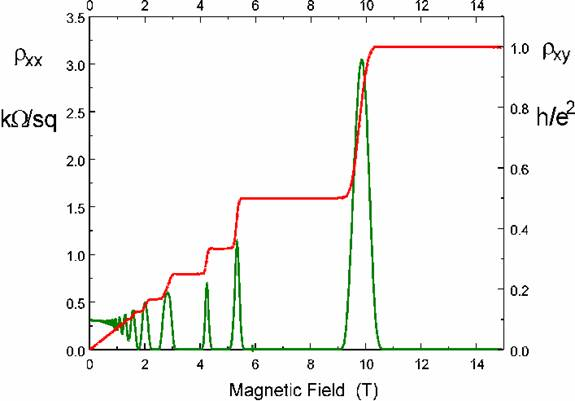
\includegraphics[width=0.5\linewidth]{images/QuantumHall}
	\caption{von Klitzing won the Nobel Prize in 1985 for discovering the quantum Hall effect evidenced by the above platueas. The green lines show $\rho_{xx}$ and the red $\rho_{xy}$. }
		
		%from http://www.referatele.com/referate/fizica/online4/HALL-EFFECT---Explanation-of-the-Quantum-Hall-Effect-referatele-com.php$
	
	\label{fig:quantumhall}
\end{figure}

Laughlin has a good charge pump argument for this quantization. A material exhibiting this behavior with $\nu = $ some integer at some specific magnetic field could be placed on a cylinder of radius R with periodic boundary conditions. Using the coordinate x = x + R for the azimuthal direction and y between 0 to L for the vertical direction, the allowed momentum around the cylinder is quantized as $k_x= 2\pi n/R$ for n an integer. Then if an extra flux $\Phi$ goes through the cylinder, the vector potential can be chosen as $A(\theta,y) = (By+\Phi /R)\hat{x}$. Of note is that the $By$ term gives a magnetic field B in the z direction, which in this case is the radial direction. This is the magnetic field through the material. The constant $\Phi/R$ just gives increases the flux through the cylinder by $\Phi$. This gives the Hamiltonian 
\begin{align}
H = \frac{p_y^2 +(p_x-eA)^2}{2m} = \frac{p_y^2 +(\hbar k_x - eA)^2}{2m} \\
= \frac{p_y^2}{2m} +\frac{(\hbar 2\pi n/R-eBy-e\Phi /R )^2}{2m}\\
= \frac{p_y^2}{2m} +\frac{(eB)^2}{2m}(y-\frac{hn}{eBR}+\frac{\Phi }{RB} )^2
\end{align}
Which is easily recognized as the simple harmonic oscillator Hamiltonian, just with y shifted by $\frac{hn}{eBR}+\frac{\Phi }{RB}$ or $(n-\frac{e\Phi}{h})\frac{h}{eBR}$, with $\frac{1}{2}m\omega^2 = \frac{(eB)^2}{2m}$
Notice that if $\Phi$ is shifted by $h/e$, that is the same as replacing n with n+1 in the Hamiltonian. This is what defines the flux quantum $\Phi_0$. So the spectrum is a series of states that are free in the x direction, and harmonic oscillators in the y direction, each one centered at some y that depends on the momentum in the x direction. If a flux quantum is added through the cylinder, that moves all the quantum states vertically by one spacing; it acts like an incompressible liquid. This essentially moves charge from one end of the cylinder to the other end. Since there is an integer number of filled harmonic oscillator states on each oscillator center, and the Hamiltonian goes back to itself after increases $\Phi$ by $\Phi_0$, this means an integer number of electrons has been moved. Now $\Delta Q = I \Delta T = \sigma_{xy}E \Delta T = \sigma_{xy} \Delta \Phi = \sigma_{xy} h/e = \nu \frac{e^2h}{he} = \nu e $ . This argument shows that $\nu$ is an integer and thus explains the integer quantum Hall effect! If one of the edges of the cylinder is shrunken to a point, then that is the point where the flux goes through. If charge is pumped to it by changing the flux, there will be some electrons bound to the flux at a general point in a 2D material. Since it is localized, it is in some sense a composite particle, and may have interesting properties.

\subsection{What is the fractional quantum Hall effect?}

The extrapolation of this to the fractional quantum Hall effect is actually quite simple. In the case where $\nu$ is a fraction, with the same set up as the previous charge pump problem where the flux through the cylinder is changed from $\Phi$ to $\Phi + \Phi_0$, the same results are derived. The difference is a charge of $\nu e$ has been moved from one side to another which is now not an integer number of electrons. Since this has been done adiabatically, this is an eigenstate. This implies that there exist local excitations that have a fractional amount of charge. Of course, these states are built out of electrons, and are just parts of a many-body electron wave functions. Again when one edge of the cylinder is shrunken to a point, then the state is tied to a flux. Then there is a fully movable local quasiparticle with fractional charge and flux. Another important consequence is described through particle exchange. Normally if two fermions are exchanged, the wavefunction picks up a sign, or a phase of $\pi$. If they were two bosons the phase is 0. Here there is a fractional charge though, so there is no reason for that to hold. If these two excitations are braided, or exchanged twice, or topologically equivalent to having one particle make a circle around the other and return to its original position, there can be some phase when compared to moving around the same circle without the second particle in the center. It is called braiding since the world line of these particles looks exactly like a braid. In 3 dimensions or higher, if a particle is braided around another, that is topologically equivalent to doing nothing, but in 2 dimensions, in general there are an integer number of classes of distinct topological paths, corresponding to how many times on particle wraps around the other. This is why you can get complex braiding phases. Particle statistics are in a sense, a representation of the braid group acting on the wavefunction. Back to our case, if there is one stationary quasiparticle tied to a quantum of flux, and then another particle of charge $e\nu$ moved around it, then there will be an phase of $e\nu\Phi_0/\hbar$ or $2\pi\nu$. That means the exchange phase has to be $\pi \nu$ which if $\nu$ is a fraction is completely new. The topological spin $h$ is defined in terms of these braiding phases, with $\theta_{a}=e^{2\pi i h}$, where $\theta_{a}$ is the exchange phase of a with a. As a sanity check, a fermion with spin 1/2 has a -1 phase and bosons of spin 0 have a phase of 1. This is why these quasiparticles are called anyons, as opposed to fermions and bosons, since they can in principle have "any" spin. 

Laughlin described a trial wavefunction that approximates well the $\nu = 1/q$ ground state, which gives $> 99\%$ overlap with the numerically calculated ground state.

Laughlin's wave function is 
\begin{align}
\Psi(z_1,z_2,...,z_n) = \prod_{j<k}(z_j-z_k)^q \exp^{-\sum_i(|z_i|^2eB/4\hbar)}
\end{align} 
The form can be guessed by assuming it has a "Jastrow" form component $\prod_{j<k}f(z_j-z_k)$, which is translation invariant, and takes into account two body interactions. The exponential term localizes each electron. Notice that q has to be odd in order for the wavefunction to be antisymmetric. Laughlin also described an operator which locally creates the excitation at $z_0$ with -1/q charge, or removes a flux quanta, which is just $\prod_{j<k}(z_j-z_0)$. This can be used to find out the braiding statistics, and the charges. It can be easily guessed however that since an electron adds a  $\prod_{j<k}(z_j-z_0)^q$, along with an exponential suppression, that this operator is just 1/q of that. There is experimental evidence of these fractional charges\cite{1997Natur.389..162D}. Haldane and later Halperin showed that if there is a Laughlin state, some of the excitations can be used to create another Laughlin state; much like how the Laughlin state is made of electron operators. This yeilds filling fractions of any odd denominator. These are called hierarchy states. 

There is a basic picture to understand what is happening here described by Jain. $\nu = \frac{nh}{eB}$, but $\frac{h/e}{BA}$ where A is the area of the state, is one over the number of flux quantums, and n is the density of electrons. That means $\nu = \frac{nhA}{eBA} = \frac{nA}{\#\Phi_0} = \frac{\#elec}{\#\Phi_0}$. So the fraction really describes a ratio between fraction of electrons to flux quanta. The idea is to make a non interacting composite system. Electrons don't interact with even amounts of fluxes, since they get $\pi$ phases around one, or $2\pi$ with 2. To recreate our original state out of just composite fermions and a magnetic field, there must be the same filling fraction $\nu$, or $\nu$ electrons for each flux for these composites. So the density $\nu$ per flux of composites is necessary to get the correct charge, but a density of $2m\nu$ of fluxes on top of the external flux is necessary to cancel out the even number of fluxes attached to the composites. So then each composite sees a magnetic flux density of $2m\nu+1$. An integer quantum Hall state with filling $p = \frac{\nu}{2m\nu+1}$ can be created out of composites, which corresponds to an original state with a filling fraction for electrons of $\nu = \frac{p}{2mp-1}$. The integer quantum Hall state is already a non compressible non interacting liquid, so this functions as a model for the fractional state. 

Another interesting fact about fractional quantum Hall states is when they are placed on a torus, there is ground state degeneracy. If a flux and an antiflux are introduced at some point, they can go around one of the nontrivial torus loops and annihilate. Now label the 2 different ways you can do this by $T_1$ and $T_2$. It is possible to act with the operators in the following way, $T_1^{-1}T_2^{-1}T_1T_2$, which is the commutator of these 2 operators. Now after a T operator has acted, there is left behind a flux line that loops around the torus. In general these fluxes can braid, which means their commutator is in general non-zero. Yet, these T operators certainly commute with the Hamiltonian. This means if the state starts in a ground state that is also an eigenstate of $T_1$, $|\psi>$, and goes to $T_2|\psi>=e^{i\theta}|\psi>$ under $T_2$, that would mean the T's commute. However they don't so $T_2$ must bring the system to a distinct ground state, i.e. topological ground state degeneracy. In general the braiding phases mentioned earlier, don't just have to be a phase, since they act on now a vector space of ground states, i.e. it could be a represented as a matrix on the space of ground states. This is known as a non Abelian topological phase.

The formulation of two very special things happened in this section; quasiparticles with fractional charge and with fractional statistics. Regarding the problem of classifying fractional quantum Hall states, one could look at either symmetries or topological invariants. If two states have topologically distinct quasiparticles, then they are definitely different phases, since the braiding rules would not change continuously. Even if the restriction to the class without symmetry in just 2 dimensions is considered, there could possibly be a fantastic number topologically distinct quasiparticles, thrown into an even larger size of different states. It turns out there are rules that govern what types of quasi-particles you can have, like locality and unitarity, that place this into the branch of mathematics called modular tensor category theory. Even then this is not a solved problem. This is very abstract still, since only a few of the many possible states allowed by modular tensor category theory have been experimentally realized, and many of those states can be well understood using the composite description above.

\subsection{The Pfaffian states}

So of interest in this work is not an odd denominator state, but even. It would be useful to be able to have an operator that is like half of the electron creation operator. The reason being that for the Dirac semimetal paper~\cite{RazaSirotaTeo17}, the Dirac electrons could be written as $v=1/2$ operators, and then possibly interactions with these operators can gap the semimetal in a symmetric way that the original electron operators could not. That would be inherently a many body phase, since these operators must be built of parts of manybody electron wavefunctions.  This is precisely the solution this paper is looking for.

The Moore Read state~\cite{MooreRead,ReadMoore,GreiterWenWilczekPRL91,GreiterWenWilczek91} provides a possible description of a $v=5/2$ state. The first two Landau levels are inert, so just the half filled third level is considered. Notably these states then have $v=1/2$ theoretically, even though there is no $v=1/2$ state experimentally. The two "inert" Landau levels are actually vital to the states existence, but the resulting ground state of this approximation seem to match well with the $v=5/2$ state. Essentially there is the same composite fermion description, i.e. two fluxes for each electron. Now instead of making an integer quantum Hall state with them, which would only yield odd denominator filling fractions, just like in superconducting theory, they combine to make a "Cooper pair" and then open up a "superconducting" gap, or a nonzero energy cost to create excitations. This can create a gap in a number of ways, which gives rise to many possible states. Since these are not actual electrons it does not mean the actual state is superconducting. In particular Moore and Read wrote down a trial wave function very similar to the Laughlin wavefunction.

In order to know how they got this wavefunction, some conformal field theory is necessary. Conformal field theory will be useful later, so there will be a brief overview here.

\subsubsection{Conformal Field Theory and Chern-Simons Theory Aside}
Conformal field theory evolved from string theory. It describes field theories that have a conformal symmetry, which is a spatial/time transformation that leaves the metric $g_{\mu \nu}$ unchanged up to multiplying it by a constant. It turns out that in 1+1 dimensions, at a critical point, if there is a local Lagrangian there is a conformal symmetry. Even for non critical theories such as fractional quantum Hall theories, if they are Abelian they are described by a Chern-Simons theory. Witten showed the Chern-Simons 2+1 d excitations correspond to primary fields on the edge. Abelian Chern-Simons theories describe most of fractional quantum Hall states, and there is powerful formalism for them. The Abelian Chern-Simons term is a gauge invariant term in 2+1 dimensions, 
\begin{align}
\mathcal{L}_{CS} = \frac{1}{4\pi}\varepsilon^{\mu \nu \lambda }K_{IJ}a_\mu^I\partial_\nu a^J_\lambda -e A_\mu t_I \partial_\nu a^I_\lambda \varepsilon^{\mu \nu \lambda }
\end{align}
Which corresponds to 1+1 d conformal field theory of 
\begin{align}
\mathcal{L}_{CFT} = \frac{1}{2\pi}\partial_t\phi^I K_{IJ} \partial_x\phi^J + ...
\end{align}

Where the NxN coupling matrix K is creatively called the "K matrix", $a$ and $\phi$ are N component U(1) gauge fields, A is the electromagnetic gauge field and the coupling t is a called the charge vector. K must be integer valued to be gauge invariant. The low energy excitations of this theory are given by the potential energy, meaning not just any combinations of $\phi$'s are there. This matrix follows through to the conformal field theory, and together with the charge vector, can be used to calculate what all the excitations are in terms of the fields, their fusion rules and their braiding statistics. The K matrix defines an integer anyon lattice $\Gamma^*=\mathbb{Z}^N$, where a vector $b=(b_1,b_2,...b_N)$ corresponds to a creation operator of an anyon $\psi_b=e^{i b \cdot \phi}$ on the ground state. Fusion then is just vector addition in this lattice. The charge of this anyon is given by $q_a = t^TK^{-1}a$. Many of these particles are local bosons, specifically, any excitations given by $K\mathbb{Z}^N$ do not braid with anything, so anyons are typically considered mod any local boson, or just anyons in $\mathbb{Z}^N/K\mathbb{Z}^N$, which contains det|K| elements. The canonical commutation relations of the Lagrangian give the commutation relations for the creation and annihilation operators for these fields. This gives the exchange phases and hence braiding. The braiding phase of anyons a around b is $\theta_{a,b} = e^{2\pi i a^T K^{-1} b}$, and the topological spin of a particle is defined by a 360 twist, or equivalently the phase it is exchanged with itself, i.e., half a braiding phase. This goes as follows: $\theta_a=\sqrt{\theta_{a,a}} = e^{\pi i a^T K^{-1} a} = e^{2 \pi i h_a}$ or $h_a = a^T K^{-1} a /2$ mod 1. It can be checked that an exchange phase of -1 corresponds to spin 1/2. Notice also that braiding and fusion are related. If a 360 twist is done on particle c, and c = a x b, this is also braiding a around b, with a 360 twist of a and b. The $2\pi$ monodromy phase $\mathcal{M}^{XY}_Z=R^{XY}_ZR^{YX}_Z$ between primary fields $X$ and $Y$ with a fixed overall fusion channel $Z$ can be deduced by the {\em ribbon identity}~\cite{Kitaev06}: \begin{align}e^{2\pi ih_Z}=\vcenter{\hbox{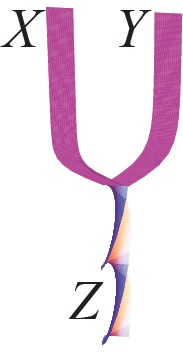
\includegraphics[width=0.5in]{ribbon1.jpg}}}=\vcenter{\hbox{
\includegraphics[width=0.5in]{ribbon2.jpg}}}=\mathcal{M}^{XY}_Ze^{2\pi i(h_X+h_Y)}\label{ribbonapp}\end{align} for $h_{X,Y,Z}$ being the conformal spins for primary fields $X,Y,Z$. Unlike the gauge-dependent $\pi$-exchange phase $R^{XY}_Z$, the $2\pi$-monodromy phase $\mathcal{M}^{XY}_Z=e^{2\pi i(h_Z-h_X-h_Y)}$ is gauge independent and physical. This means with just the spins and fusion rules the braiding statistics can be derived. Not only that but $\sigma_{xy}$ can be calculated as $tK^{-1}t$  in units of the quantum conductance. This is consistent with the Laughlin theory having a K matrix of 3, and a charge vector of 1. Here is a summary of these important formulas.

\begin{align}
\theta_{a,b} = e^{2\pi i a^T K^{-1} b} \label{eq:transform1}\\
h_a = a^T K^{-1} a /2 \mod 1 \label{eq:transform2}\\
\theta_{a,b}= h_{a\times b}-h_a-h_b  \label{eq:transform3}\\
q_a = t^TK^{-1}a \label{eq:transform4}\\
\sigma_{xy} = t^TK^{-1}t \label{eq:transform5}
\end{align}

A change of basis gives new matrices described by the following 
\begin{align}
\tilde{\phi}=M\phi \quad M^T\tilde{K}M=K \quad \tilde{t}=Mt
\end{align}

Notably, not all theories are Abelian. There are non-Abelian Chern-Simons theories, they are not so straightforward to describe. Here is a description of the general structure of conformal field theory.  For a more in depth introduction, see {\color{red}cite this} http://www.damtp.cam.ac.uk/ user/tong/string/four.pdf. 

In two dimensions, conformal field theory typically uses $z = t + ix$  and $\bar{z}= t - ix$ instead of using space and time coordinates because conformal transformations then take the form $z \rightarrow f(z)$ and $\bar{z} \rightarrow \bar{f}(\bar{z})$. In this way the theory splits into just the z or $\bar{z}$ dependent pieces. The infinitesimal form of this is $z \rightarrow z + \epsilon(z)_n$ where $\epsilon(z)_n = -z^{n+1}$, which is generated by $l_n = -z^{n+1}\partial_z$. $l_0+\bar{l}_0$ and $i(l_0-\bar{l}_0)$ generate scaling and rotations. In a quantum theory, infinitesimal transformations can be generated using the stress energy tensor, and there may be some nontrivial commutation. In conformal theories, the stress energy tensor also breaks up into two parts, $T_{zz}(z)$ and $T_{\bar{z}\bar{z}}(\bar{z})$, with $T_{zz} =T_{\bar{z}\bar{z}}=0$. If the stress energy tensor is broken into moments, $L_n$ they will follow similar commutation relations as $l_n$, except there is an extra piece called the central charge on the commutation of $L_n$ and $L_{-n}$. Their algebra is called the Virasoro algebra.

There is a notion of primary fields, which transform a specific way under a conformal transformations, $ \Psi(z,\bar{z}) \rightarrow (\frac{\partial f}{\partial z})^h (\frac{\partial \bar{f}}{\partial \bar{z}})^{\bar{h}}  \Psi(f(z),\bar{f}(\bar{z}))$, where $h$ and $\bar{h}$ are called the conformal weights. These are important to remember since they are eigenstates of scaling and rotations. $h-\bar{h}$ is the spin eigenvalue and $h+\bar{h}$ is the eigenvalue of scaling. That also makes them eigenstates of Virasoro operators $L_n$, or a representation of the algebra. This is a little different then typical field theory, where we call the functions we integrate the path integral over fields, here a field is just any function.

The next important piece is the operator product expansion. The correlator of two local operators, $<O_1(z,\bar{z})O_2(w,\bar{w})>$ can be expressed by taking a Taylor expansion as w approaches z. The operator product expansion is defined as
\begin{align}
<O_i(z,\bar{z})O_j(w,\bar{w})...> = \sum_k C^k_{ij}(z-w,\bar{z}- \bar{w}) <O_k(w,\bar{w})...>
\end{align}
Where the sum is over all local operators. The ... part refers to the idea that this holds when these are followed by a string of other operators, as long as they are not close to z or w relative to the distance between them. The form of these C functions are restricted since there is conformal symmetry. For example they must only depend on position differences due to translation symmetry. If the local excitations in the quantum Hall effect are the local operators, then their operator product expansion would give information about their fusion rules, i.e., what other local operators their sum is described by. Something familiar to this are the Clebsch–Gordan coefficients. This looks much like an algebra, but because of its z dependence is given the name vertex algebra. It actually contains more information than fusion rules. If the operators are primary they are restricted to only have two divergent parts, with one proportional to the conformal weight. The operator product expansion can be used to define primaries as well.

The operator product expansion of the stress energy tensor with itself, which is notably not primary, will get not just a weight term, but a $1/(z-w)^4$ term proportional to what is called the central charge. The local operator with this piece is just the identity, so it adds some zero energy to your theory. That energy is also known as a Casimir energy. There is a theorem that says that the central change counts your degrees of freedom, and is related to the total heat current. For example $c=\bar{c}=n$ for n scalar fields (bosons), and $c=\bar{c}=n/2$ for n free fermion fields.

Finally there are rational conformal field theories. These are theories where you can get all of the possible fields from a finite number of primary fields. The generators are representations of the Virasoro algebra. By acting on them with "lowering" operators, their conformal weights can be changed. The rational conformal field theories are completely solvable given just symmetry arguments. A good analogy here are the spin states, where given a highest spin, by acting with lowering operators all possible states can be described. At some point the sequence will terminate.

Moore and Read found a way to write the Laughlin wavefuntion as a correlator of fields. Then they used that same prescription to find a wave function for a $\nu=1/2$. The real wavefunction would be this on top of the wavefunction of two completely filled Landau levels. 
\begin{align}
\Psi(z_1,z_2,...,z_n) = Pf(\frac{1}{z_i-z_j})\prod_{j<k}(z_j-z_k)^2 \exp^{-\sum_i(|z_i|^2eB/4\hbar)}
\end{align}

Where $Pf$ is the Pfaffian of a skew-symmetric matrix. It is defined as a polynomial in the matrix entries with integer-valued coefficients such that $Pf(M)^2=det(M)$. The term falls out of Wicks theorem when it is applied to real fermion fields. The important thing about this term is that it lets the wavefunction be antisymmetric when q is even. Using this ground state, the elementary excitations can be found. Since the electrons or composite fermions are paired, when a flux is braided around them the resulting phase is doubled. This means the flux quantum is halved. So now in the charge pump argument the elementary excitation has charge $\nu e/2 = e/4$, modulo e. The braiding statistic of this particle with the electron is 1, and its spin $h$, which is defined by the phase of braiding it around another copy of itself, $e^{2\pi i h}$, is $1/16$. This primary field also ends up being non-Abelian, i.e., the operator product expansion with itself gives a two primary fields, a fermion and a boson with charge e/2. In this way all the excitations are produced. This Moore-Read state can be described as a decomposition into $Ising \otimes U(1)_4$ Where the $U(1)_4$ is just particles of charge $ne/4$, where n is an integer from 0 to 7, called $e_1,e_2,...e_7$, and the Ising theory is the Majorana fermion $\psi$, and the $\pi$ flux $\sigma$, where anything that is not local with respect to the electron is removed. The excitations topological spins are described in Table ~\ref{tab:Pfaff}.
\begin{table}[h]
	\centering
	\begin{tabular}{|c|c|c|c|c|c|c|c|c|}
		\hline
		&$e_0$& $e_1$ & $e_2$ & $e_3$ & $e_4$& $e_5$& $e_6$& $e_7$\\
		\hline
		$\openone$ & 0 && 1/4 & & 0 && 3/4 & \\
		\hline
		$\sigma $ && 1/8 && 5/8 && 5/8 && 1/8 \\
		\hline
		$\psi$ & 1/2 && 3/4 & & 1/2 && 1/4 &\\
		\hline
		charge & 0 &e/4& 2e/4 & 3e/4 & e & 5e/4& 6e/4 & 7e/4\\
		\hline
	\end{tabular}
	\label{tab:Pfaff}
	\caption{The topological spins of the Pfaffian state}
\end{table}

Much of what follows now until the end of this section is a direct exert from one of the papers this thesis is based upon~\cite{RazaSirotaTeo17} that make some important clarification valuable at this point in the discussion. It is important to clarify and disambiguate the three "Pfaffian" fractional quantum Hall states that commonly appear in the literature. All these $(2+1)$D states are theorized at filling fraction $\nu=1/2$, although are applied to $\nu=5/2$ in materials, and have identical electric transport properties. However, they have distinct thermal Hall transport behaviors. They all have very similar anyonic quasiparticle structures. For instance, they all have four Abelian and two non-Abelian quasiparticles (up to the electron). On the other hand, the charge $e/4$ non-Abelian Ising anyons of the three states have different spin-exchange statistics. First, the gapless boundary of the Moore-Read Pfaffian fractional quantum Hall state can be described by the $(1+1)$D chiral conformal field theory $U(1)_4\otimes\mathrm{Ising}$ where the charged boson and neutral fermion sectors are co-propagating. It therefore carries the chiral central charge $c=1+1/2=3/2$, which dictates the thermal Hall response \eqref{conductance}. Second, the "anti-Pfaffian" fractional quantum Hall state~\cite{LevinHalperinRosenow07,LeeRyuNayakFisher07} is the particle-hole conjugate of the Moore-Read Pfaffian state. Instead of half-filling the lowest Landau level by electrons, one can begin with the completely filled lowest Landau level, and half-fill it with holes. In a sense the anti-Pfaffian state is obtained by subtracting the completely filled lowest Landau level by a Moore-Read Pfaffian state. Along the boundary, the $(1+1)$D conformal field theory $U(1)_{1/2}\otimes\overline{U(1)_4\otimes\mathrm{Ising}}$ consists of the forward propagating chiral Dirac $U(1)_{1/2}$ sector that corresponds to the lowest Landau level, and the backward propagating Moore-Read Pfaffian $\overline{U(1)_4\otimes\mathrm{Ising}}$. Here $\overline{\mathcal{C}}$ can be interpreted as the time-reversal conjugate of the chiral conformal field theory $\mathcal{C}$. The thermal transport is governed by the edge chiral central charge $c=1-3/2=-1/2$, which has an opposite sign from the filling fraction. Thus, unlike the Moore-Read Pfaffian state, the net electric and thermal currents now travel in opposite directions along the edge. Lastly, the recently proposed particle-hole symmetric Pfaffian state~\cite{Son15,BarkeshliMulliganFisher15,WangSenthil16}, which is going to be the {\em only} Pfaffian fractional quantum Hall state considered here (see Ref.~\onlinecite{KaneSternHalperin17} for a coupled wire construction), has the chiral edge conformal field theory \eqref{PfaffianCFT}. As the electrically charged boson and neutral fermion sectors are counter-propagating, the net thermal edge transport is governed by the chiral central charge $c=1-1/2=1/2$. The chiral $(1+1)$D particle hole symmetric Pfaffian conformal field theory \eqref{PfaffianCFT} is also present along the line interface separating a time reversal symmetric $\mathcal{T}$-Pfaffian~\cite{ChenFidkowskiVishwanath14} domain and a time reversal breaking magnetic domain on the surface of a 3D topological insulator. (Similar constructions can be applied to alternative time reversal symmetric topological insulator surface states~\cite{WangPotterSenthilgapTI13,MetlitskiKaneFisher13b,BondersonNayakQi13}, but they will not be considered here.) Other than their thermal transport properties, the three Pfaffian fractional quantum Hall state can also be distinguished by the charge $e/4$ Ising anyon, which has spin $h=1/8$, $-1/8$ or $0$ for the Moore-Read Pfaffian, anti-Pfaffian or particle hole symmetry Pfaffian states respectively. 

Since this thesis will not be considering the Moore-Read Pfaffian or its particle-hole conjugate anti-Pfaffian state, the particle hole symmetry Pfaffian state will be refered to simply as the Pfaffian state. It is actually true that there are other Abelian theories that describe a $\nu=1/2$ state, but this thesis does not work with them.

\subsection{Pfaffian Field Theory}
The reason why there is such focus on this Pfaffian state is that many-body interactions can facilitate the fractionalization of a $(1+1)$D chiral Dirac channel \begin{align}\mathrm{Dirac}=\mathrm{Pfaffian}\otimes\mathrm{Pfaffian}\label{fractionalization}\end{align} (see also figure~\ref{fig:glueingsplitting}). In a sense, each chiral Pfaffian channel carries half of the degrees of freedom of the Dirac. For instance, it has half the electric and thermal conductances, which are characterized by the filling fraction $\nu=1/2$ and the chiral central charge $c=1/2$ in \eqref{conductance}. Through out this theis there are references to the low-energy effective theory that consists of an electrically charged $U(1)_4$ bosonic component,conformal field theory say moving in the $R$ direction, and a neutral Majorana fermion component moving in the opposite $L$ direction -- simply as a Pfaffian conformal field theory \begin{align}\mathrm{Pfaffian}=U(1)_4\otimes\overline{\mathrm{Ising}}.\label{PfaffianCFT}\end{align} This thesis follows the level convention for $U(1)$ in the conformal field theory community~\cite{bigyellowbook}. The same theory may be more commonly referred to as $U(1)_8$ in the fractional quantum Hall community. For clarification, see Lagrangian \eqref{Pfaffian} and \eqref{LFQHCS}.)

The low-energy effective chiral $(1+1)$D conformal field theory takes the decoupled form between the boson and fermion \begin{align}\mathcal{L}_{\mathrm{Pfaffian}}&=\mathcal{L}_{\mathrm{charged}}+\mathcal{L}_{\mathrm{neutral}}\label{Pfaffian}\\&=\frac{8}{2\pi}\partial_t\phi_R\partial_x\phi_R+v(\partial_x\phi_R)^2\nonumber\\&\;\;\;+i\gamma_L(\partial_t-\tilde{v}\partial_x)\gamma_L\nonumber\end{align} where $\hbar$ has been set to 1. Here $\phi_R$ is the free chiral $U(1)_4$ boson. It generates the $(1+1)$D theory $\mathcal{L}_{\mathrm{charged}}$, which is identical to the boundary edge theory of the $(2+1)$D bosonic Laughlin $\nu=1/8$ fractional quantum Hall state described by the topological Chern-Simons theory~\cite{WenZee92,Wenedgereview} \begin{align}\mathcal{L}_{2+1}=\frac{K}{4\pi}\alpha\wedge d\alpha+et\alpha\wedge dA\label{LFQHCS}\end{align} with $K=8$ and $t=2$. The $U(1)_4$ conformal field theory carries the electric conductance $\sigma=tK^{-1}t=1/2$ in units of $2\pi e^2=e^2/h$ and a thermal conductance characterized by the chiral central charge $c=c_R=1$. Primary fields are of the form of (normal ordered) chiral vertex operators $:e^{im\phi_R}:$, for $m$ an integer, and carries charge $q=m/4$ in units of $e$ and conformal scaling dimension (i.e.~conformal spin) $h=h_R=m^2/16$. Here is a summary and abbreviation the operator product expansion \begin{align}e^{im_1\phi_R(z)}e^{im_2\phi_R(w)}=e^{i(m_1+m_2)\phi_R(w)}(z-w)^{m_1m_2/8}+\ldots\end{align} by the Abelian fusion rule \begin{align}e^{im_1\phi_R}\times e^{im_2\phi_R}=e^{i(m_1+m_2)\phi_R},\end{align} where $z\sim\tau+ix$ is the complex space-time parameter and $\tau=i\pi vt/2$ is the Euclidean time.

$\gamma_L^\dagger=\gamma_L$ is the free Majorana fermion. It generates the $(1+1)$D theory $\mathcal{L}_{\mathrm{neutral}}$, which is equivalent to a chiral component of the critical Ising conformal field theory or the boundary edge theory of the $(2+1)$D Kitaev honeycomb model~\cite{Kitaev06} in its B-phase with time reversal breaking (i.e.~a chiral $p_x+ip_y$ superconductor coupled with a $\mathbb{Z}_2$ gauge theory). It carries trivial electric conductance but contributes to a finite thermal conductance characterized by the chiral central charge $c=-c_L=-1/2$. The Ising conformal field theory has primary fields $1$, $\gamma_L$ and $\sigma_L$, where the twist field (or Ising anyon) $\sigma_L$ carries the conformal spin $h=-h_L=-1/16$. Again, the operator product expansions go as \begin{gather}\gamma_L(\bar{z})\gamma_L(\bar{w})=\frac{1}{\bar{z}-\bar{w}}+\ldots\nonumber\\\sigma_L(\bar{z})\gamma_L(\bar{w})=\frac{\sigma_L(\bar{w})}{(\bar{z}-\bar{w})^{1/2}}+\ldots\nonumber\\\sigma_L(\bar{z})\sigma_L(\bar{w})=\frac{1}{(\bar{z}-\bar{w})^{1/8}}+(\bar{z}-\bar{w})^{3/8}\gamma_L(\bar{w})\nonumber\end{gather} by the fusion rule \begin{gather}\gamma_L\times\gamma_L=1,\quad\sigma_L\times\gamma_L=\sigma_L\nonumber\\\sigma_L\times\sigma_L=1+\gamma_L,\end{gather} where $\bar{z}\sim\tau-ix$ is the complex space-time parameter and $\tau=i\tilde{v}t$ is the Euclidean time. 

General primary fields of the Pfaffian conformal field theory decompose into the $U(1)_4$ part and the Ising part. They take the form \begin{align}1_m=e^{im\phi_R},\quad\psi_m=e^{im\phi_R}\gamma_L,\quad\sigma_m=e^{im\phi_R}\sigma_L.\label{Pfaffianfields}\end{align} The conformal spins and fusion rules also decompose so that \begin{align}h_{1_m}=\frac{m^2}{16},\quad h_{\psi_m}=\frac{m^2}{16}+\frac{1}{2},\quad h_{\sigma_m}=\frac{m^2-1}{16}\end{align} modulo 1, $q_m=m/4$ in units of $e$, and \begin{gather}1_{m_1}\times1_{m_2}=\psi_{m_1}\times\psi_{m_2}=1_{m_1+m_2}\nonumber\\1_{m_1}\times\psi_{m_2}=\psi_{m_1+m_2}\nonumber\\1_{m_1}\times\sigma_{m_2}=\psi_{m_1}\times\sigma_{m_2}=\sigma_{m_1+m_2}\nonumber\\\sigma_{m_1}\times\sigma_{m_2}=1_{m_1+m_2}+\psi_{m_1+m_2}.\end{gather} 

The electronic quasiparticle is the composition $\psi_{\mathrm{el}}=e^{-i4\phi_R}\gamma_L$ so that it is fermionic and has electric charge $-1$ in units of $e$. Since electron is the fundamental building block of the system, locality of $\psi_{\mathrm{el}}$ only allows primary fields $X$ that have trivial monodromy $\mathcal{M}^{X,\psi_{\mathrm{el}}}=1$ with the electron. As a result, this restricts $1_m,\psi_m$ to even $m$ and $\sigma_m$ to odd $m$. Lastly, the coupled wire models constructed later will involve the Pfaffian channels that propagate in both forward and backward directions. The backward case is denoted by $\overline{\mathrm{Pfaffian}}$, whose Lagrangian density is the time reversal of \eqref{Pfaffian}, i.e.~replacing $R\leftrightarrow L$, $i\leftrightarrow-i$ and $\partial_t\leftrightarrow-\partial_t$. 

\subsubsection{Gluing and splitting}\label{sec:gluing}

\begin{figure}[htbp]
	\centering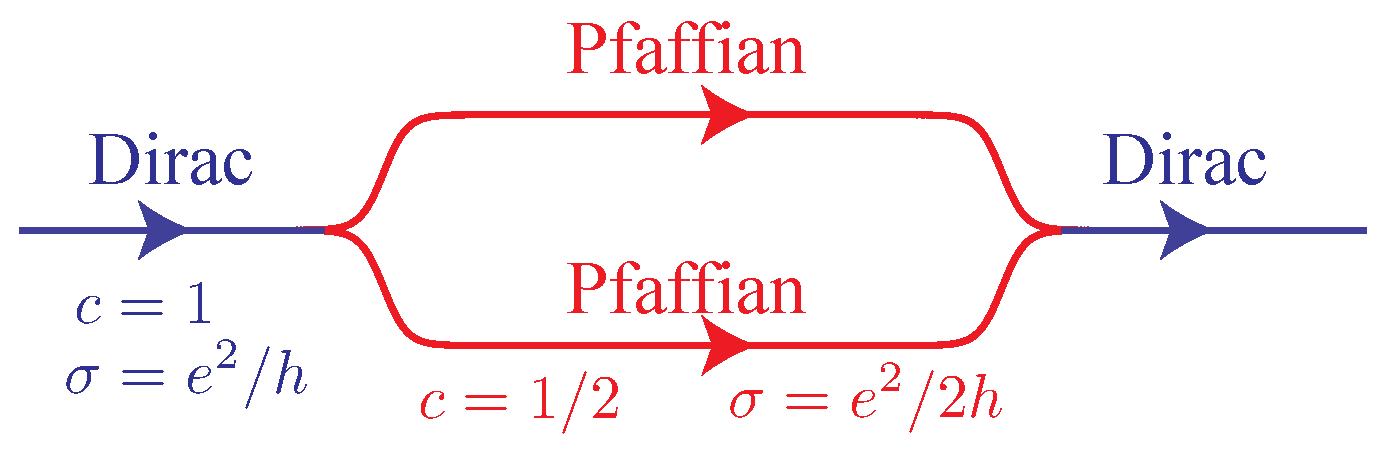
\includegraphics[width=0.3\textwidth]{glueingsplitting}
	\caption{Gluing and splitting a pair of chiral Pfaffian 1D channels into and from a chiral Dirac channel.}\label{fig:glueingsplitting}
\end{figure}

A pair of co-propagating Pfaffian conformal field theory can be "glued" together into a single chiral Dirac electronic channel. Consider the decoupled pair $\mathcal{L}_0=\mathcal{L}_{\mathrm{Pfaffian}}^A+\mathcal{L}_{\mathrm{Pfaffian}}^B$, where $\mathcal{L}_{\mathrm{Pfaffian}}^{A/B}$ is the Lagrangian density of one of the two Pfaffian conformal field theory labeled by $A,B$. The pair of Majorana fermions can compose an electrically neutral Dirac fermion $d_L=(\gamma^A_L+i\gamma^B_L)/\sqrt{2}$, which can then be bosonized $d_L\sim e^{i\phi^\sigma_L}$, for $\phi^\sigma_L$ the chiral $\overline{U(1)_{1/2}}$ boson. Bosonization can be thought of as writing a fermion in terms of a boson, which usually ends up with the form $\psi\sim e^{i\phi}$, and you can rewrite the Lagrangian with this identity, although you cannot simply plug this in because you must be careful about normal ordering. For more detail see ~\cite{Senechal99} The bare Lagrangian now becomes the multi-component $U(1)_4^A\otimes U(1)_4^B\otimes\overline{U(1)_{1/2}}$ boson conformal field theory \begin{align}\mathcal{L}_0=\frac{1}{2\pi}\partial_t\boldsymbol{\phi}^TK\partial_x\boldsymbol{\phi}+\partial_x\boldsymbol{\phi}^TV\partial_x\boldsymbol{\phi},\label{881}\end{align} where $\boldsymbol{\phi}=(\phi_R^A,\phi_R^B,\phi^\sigma_L)$, $K$ is the $3\times3$ diagonal matrix $K=\mathrm{diag}(8,8,-1)$, and $V$ is some non-universal velocity matrix. A primary field is a vertex operator $e^{i{\bf m}\cdot\boldsymbol{\phi}}$ labeled by an integral vector ${\bf m}=(m^A,m^B,\tilde{m})$. It carries conformal spin $h_{\bf m}={\bf m}^TK^{-1}{\bf m}/2$ and electric charge $q_{\bf m}={\bf t}^TK^{-1}{\bf m}$ in units of $e$, where ${\bf t}=(2,2,0)$ is the charge vector. The Haldane criterion can be used to find backscattering terms that gap out excitations~\cite{Haldane95}. The algorithm for finding them first finds null vectors, i.e.~${\bf n}^TK{\bf n}=0$.  As ${\bf n}=(1,-1,4)$ is an electrically neutral null vector (${\bf t}\cdot{\bf n}=0$), it corresponds to the charge $U(1)$ preserving backscattering coupling \begin{align}\delta\mathcal{H}=-u\cos\left({\bf n}^TK\boldsymbol{\phi}\right)=-u\cos\left(8\phi^A_R-8\phi^B_R-4\phi^\sigma_L\right)\label{glueingH}\end{align} that gaps and annihilates a pair of counter-propagating boson modes. The interacting Hamiltonian can also be expressed in terms of many-body backscattering of the Pfaffians' primary fields \begin{align}\delta\mathcal{H}=-u:\left(d_L^\dagger d_R\right)^4:+h.c.\end{align} where $d_R=1_2^A1_{-2}^B$ is the electrically neutral Dirac fermion composed of the pair of oppositely charged semions in the two Pfaffian sectors.

In strong coupling, the gapping Hamiltonian introduces an interacting mass and the ground state expectation value $\langle\Phi\rangle=n\pi/2$, for $n$ an integer and $\Phi=2\phi^A_R-2\phi^B_R-\phi^\sigma_L$. In low energy, it leaves behind the chiral boson combination $\tilde\phi_R=2\phi_R^A+2\phi_R^B$, which has trivial operator product (i.e.~commutes at equal time) with the order parameter $\Phi$. The low-energy theory after projecting out the gapped sectors becomes \begin{align}\mathcal{L}_0-\delta\mathcal{H}\longrightarrow\mathcal{L}_{\mathrm{Dirac}}=\frac{1}{2\pi}\partial_t\tilde\phi_R\partial_x\tilde\phi_R+v(\partial_x\tilde\phi_R)^2\end{align} which is identical to the bosonized Lagrangian density of a chiral Dirac fermion. For instance, the vertex operator $\psi_R^{\mathrm{el}}\sim e^{i\tilde\phi_R}\sim 1_2^A1_2^B$ has the appropriate spin and electric charge of an electronic Dirac fermion operator ($h=1/2$ and $q=1$ in units of $e$). Notice that the vertex operator $e^{i\tilde\phi_R/2}$ has $-1$ monodromy with the local electronic $\psi_R^{\mathrm{el}}$ and therefore is not an allowed excitation in the fermionic theory.

Notice that the gluing potential \eqref{glueingH} facilitates an anyon condensation process~\cite{BaisSlingerlandCondensation}, where the maximal set of mutually local neutral bosonic anyon pairs \begin{align}\begin{array}{*{20}c}1_{4m}^A1_{-4m}^B,\psi_{4m}^A\psi_{-4m}^B,\\\psi_{4m+2}^A1_{-4m-2}^B,1_{4m+2}^A\psi_{-4m-2}^B,\sigma_{4m+1}^A\sigma_{-4m-1}^B\end{array}\label{condensebosons}\end{align} is condensed, where $m$ is an arbitrary integer. All primary fields that are non-local (i.e.~with non-trivial monodromy) with any of the condensed bosons in \eqref{condensebosons} are confined. Any two primary fields that differ from each other by a condensed boson in \eqref{condensebosons} are now equivalent. The condensation therefore leaves behind the electronic Dirac fermion \begin{align}\psi^{\mathrm{el}}_R=\psi^A_4\equiv\psi^B_4\equiv1_2^A1_2^B\end{align} and its combinations. 

\begin{figure}[htbp]
	\centering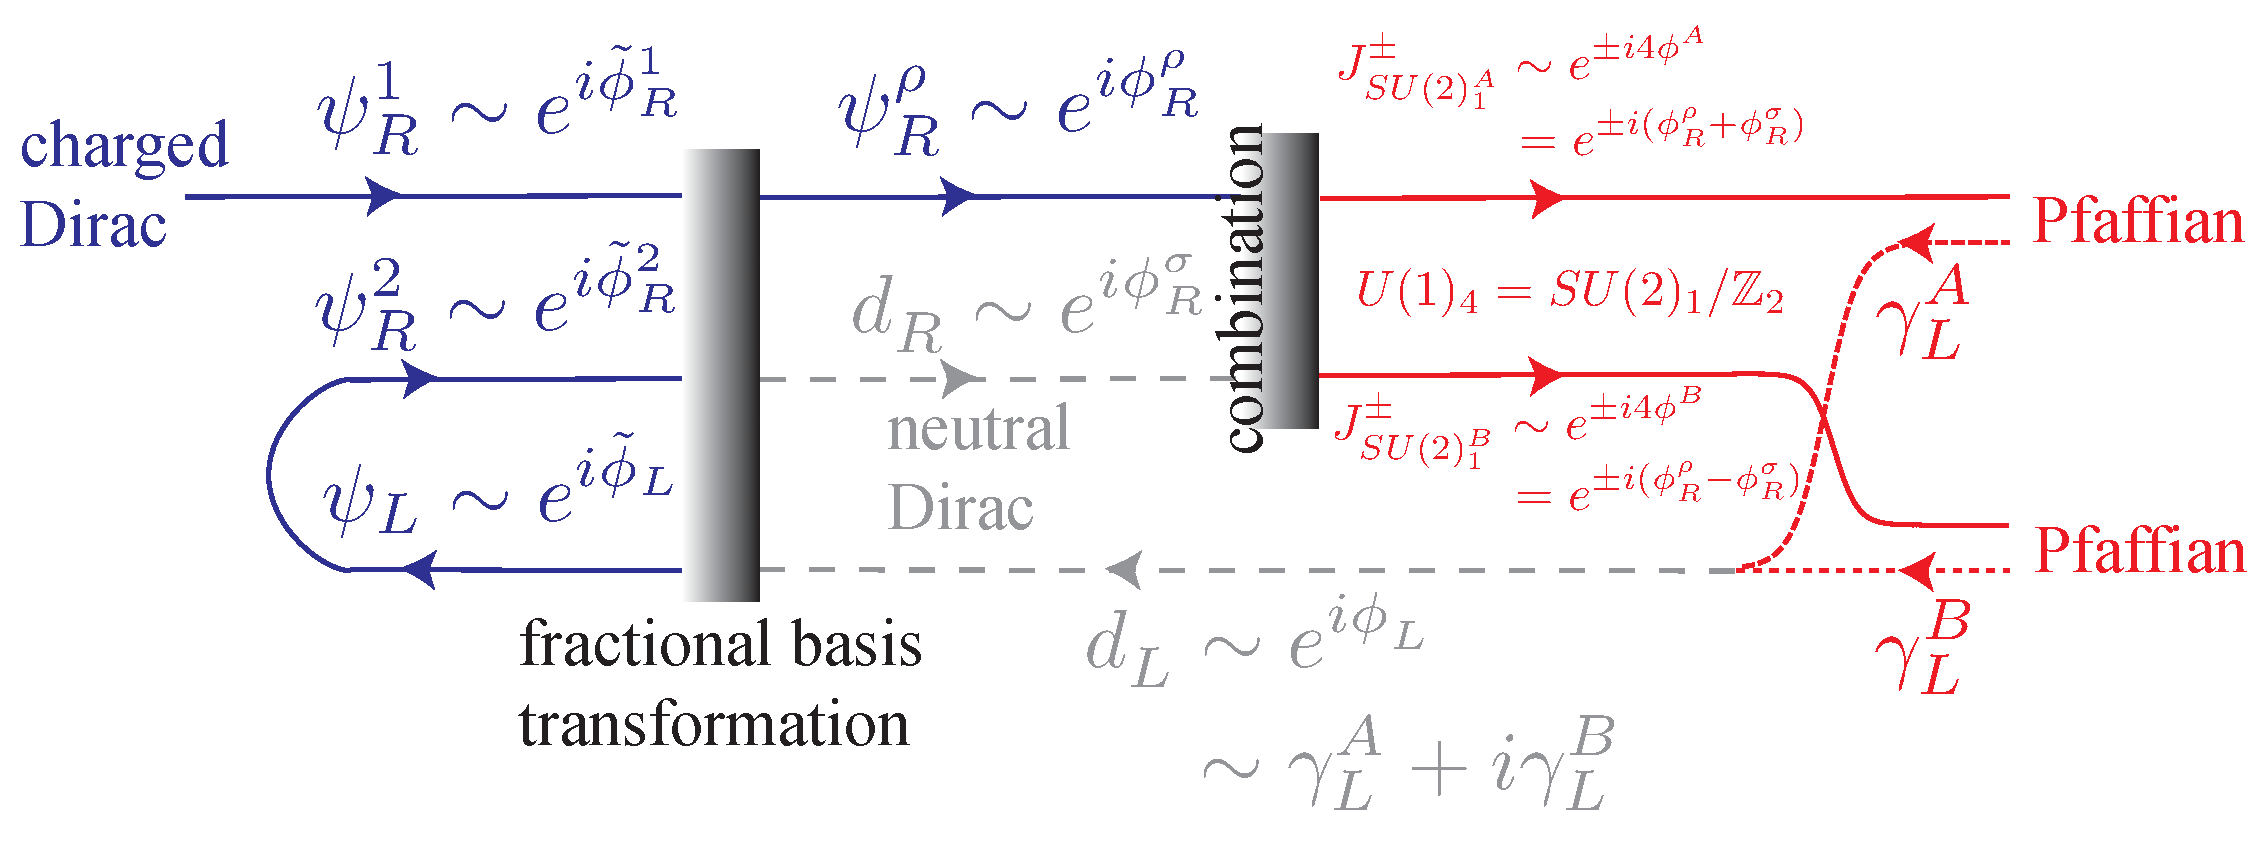
\includegraphics[width=0.5\textwidth]{fractionalization}
	\caption{Schematics of splitting a chiral Dirac channel into a pair of Pfaffian channels.}\label{fig:fractionalization}
\end{figure}

On the other hand, a chiral Dirac channel can be decomposed into a pair of chiral Pfaffian channels (see figure~\ref{fig:fractionalization} for a summary). The first problem is that the Pfaffian has many more degrees of freedom then a Dirac fermion. Perhaps from some channel re-construction, an additional pair of counter-propagating Dirac modes is appended to the chiral Dirac channel. This can be realized by pulling a parabolic electronic/hole band from the conduction/valence band to the Fermi level, or introducing non-linear dispersion to the original chiral channel. In low-energy, the three Dirac fermion modes can be bosonized $\psi^{1,2}_R\sim e^{i\tilde\phi_R^{1,2}}$, $\psi_L\sim e^{-i\tilde\phi_L}$ and they are described by the multicomponent boson Lagrangian \begin{align}\widetilde{\mathcal{L}}_{\mathrm{Dirac}}=\frac{1}{2\pi}\partial_t\widetilde{\boldsymbol\phi}^T\tilde{K}\partial_x\widetilde{\boldsymbol\phi}+\partial_x\widetilde{\boldsymbol\phi}^T\tilde{V}\partial_x\widetilde{\boldsymbol\phi}\label{3Dirac}\end{align} for $\widetilde{\boldsymbol\phi}=(\tilde\phi_R^1,\tilde\phi_R^2,\tilde\phi_L)$, $\tilde{K}$ is the diagonal matrix $\tilde{K}=\mathrm{diag}(1,1,-1)$, and $\tilde{V}$ is some non-universal velocity matrix. A general composite excitation can be expressed by a vertex operator $e^{i{\bf m}\cdot\widetilde{\boldsymbol\phi}}$, for ${\bf m}$ an integral 3-vector, with spin $h_{\bf m}=|{\bf m}|^2/2$ and electric charge $q_{\bf m}={\bf m}^T\tilde{K}\tilde{\bf t}$ in units of $e$, where $\tilde{\bf t}=(1,1,1)$ is the charge vector.

Next perform a {\em fractional} basis transformation \begin{align}\begin{array}{*{20}l}\phi^\rho_R=\tilde\phi^1_R+\tilde\phi^2_R+\tilde\phi_L\\\phi^\sigma_R=\tilde\phi^1_R-\frac{1}{2}\tilde\phi^2_R+\frac{1}{2}\tilde\phi_L\\\phi^\sigma_L=\tilde\phi^1_R+\frac{1}{2}\tilde\phi^2_R+\frac{3}{2}\tilde\phi_L\end{array}.\label{fracbasistrans0}\end{align} This follows the transformation rules from equations ~\ref{eq:transform1}~--~\ref{eq:transform5}. While the $\tilde{K}$ matrix is invariant under the transformation, the charge vector changes to $\tilde{\bf t}\to(1,0,0)$. $\psi^\rho_R\sim e^{i\phi^\rho_R}$ is the local electronic Dirac fermion that carries spin $1/2$ and electric charge $e$, and $d_{R/L}\sim e^{i\phi^\sigma_{R/L}}$ are counter-propagating electrically neutral Dirac fermions. As the $\tilde{K}$ matrix is still diagonal, these fermions have trivial mutual $2\pi$-monodromy and are local with respect to each other. However, it is important to notice that the neutral Dirac fermions $d_{R/L}$ actually consist of fractional electronic components.

Now consider the two $R$-moving Dirac channels. By pairing the Dirac fermions, they form two independent $SU(2)_1$ Kac-Moody current operators~\cite{bigyellowbook}. This is defined by the operator product expansion in equation~\ref{SU2algebra}. \begin{align}J_3^{A/B}(z)&=i2\sqrt{2}\partial_z\phi^{A/B}_R(z)\label{SU2current}\\J_\pm^{A/B}(z)&=\frac{J_1^{A/B}(z)\pm iJ_2^{A/B}(z)}{\sqrt{2}}=e^{\pm i4\phi^{A/B}_R(z)}\nonumber\end{align} where $4\phi^A_R=\phi^\rho_R+\phi^\sigma_R$ and $4\phi^B_R=\phi^\rho_R-\phi^\sigma_R$. Both $SU(2)_1$ sectors are electrically charged so that the bosonic vertex operators $J_\pm^{A/B}$ carries charge $\pm e$. They obey the $SU(2)$ current algebra at level 1 \begin{align}J^\lambda_{\mathsf{i}}(z)J^{\lambda'}_{\mathsf{j}}(w)=\frac{\delta^{\lambda\lambda'}\delta_{\mathsf{ij}}}{(z-w)^2}+\sum_{\mathsf{k}=1}^3\frac{i\sqrt{2}\delta^{\lambda\lambda'}\varepsilon_{\mathsf{ijk}}}{z-w}J^\lambda_{\mathsf{k}}(w)+\ldots\label{SU2algebra}\end{align} for $\lambda,\lambda'=A,B$. It is crucial to remember that $J_\pm^A\sim\psi^\rho_Rd_R$ and $J_\pm^B\sim\psi^\rho_Rd_R^\dagger$ contains the fractional Dirac components $d_R$. Thus, the primitive local bosons are actually pairs of the current operators, i.e.~$e^{i8\phi^{A/B}_R}$. Equivalently, this renormalizes the compactification radius of the boson $4\phi^{A/B}_R$ so that in a closed periodic space-time geometry, the electronic Cooper pair combinations such as the charge $2e$ local operators  \begin{gather}e^{i8\phi^A_R}=e^{i(4\tilde\phi^1_R+\tilde\phi^2_R+3\tilde\phi_L)}\sim(\psi^1_R)^4\psi^2_R(\psi_L^\dagger)^3\nonumber\\e^{i8\phi^B_R}=e^{i(3\tilde\phi^2_R+\tilde\phi_L)}\sim(\psi^2_R)^3\psi_L^\dagger\end{gather} are required to be periodic. The incorporation of anti-periodic boundary condition for $J_\pm^{A/B}=e^{\pm i4\phi^{A/B}_R}$ results in the $\mathbb{Z}_2$-orbifold theory~\cite{Ginsparg88,DijkgraafVafaVerlindeVerlinde99} $U(1)_4=SU(2)_1/\mathbb{Z}_2$ for both $A$ and $B$ sectors. Orbifolding usually results in new "twist" fields", or fields that when braided with the object that is can have antiperiodic boundary conditions, yeilds the -1 required. For instance, the primitive twist fields are given by $e^{\pm i\phi^{A/B}_R}$, which have $-1$ monodromy phase with $J_\pm^{A/B}$. 

At this point, including the $L$-moving neutral Dirac sector, the muticomponent boson $\boldsymbol\phi=(\phi^A_R,\phi^B_R,\phi^\sigma_L)$ described by the Lagrangian \eqref{881} has been recovered . Lastly, simply decompose the remaining neutral Dirac into Majorana components, $d_L=(\gamma^A_L+i\gamma^B_L)/\sqrt{2}$. The $A$ and $B$ Pfaffian sectors can then be independently generated by the charged $U(1)_4$ boson $\phi^{A/B}_R$ and the neutral Majorana fermion $\gamma^{A/B}_L$. As a consistency check, the charge $e$ fermionic (normal ordered) combinations defined in \eqref{Pfaffianfields} \begin{align}\psi_4^A&\sim e^{i4\phi^A_R}\gamma_L^A\sim e^{i\tilde\phi^1_R}+e^{i(3\tilde\phi^1_R+\tilde\phi^2_R+3\tilde\phi_L)}\label{psi4def1}\\\psi_4^B&\sim e^{i4\phi^B_R}\gamma_L^B\sim e^{i(-\tilde\phi^1_R+\tilde\phi^2_R-\tilde\phi_L)}-e^{i(\tilde\phi^1_R+2\tilde\phi^2_R+2\tilde\phi_L)}\nonumber\end{align} are in fact local quasi-electronic. %(The minus sign in the bosonized expression for $\psi_4^A$ comes from the Klein factors defined later in \eqref{ETcomm0} and \eqref{ETcomm1}).

Unlike in the gluing case where there is a gapping Hamiltonian \eqref{glueingH} that pastes a pair of Pfaffians into a Dirac, here in the splitting case there has been some kind of fractional basis transformation that allows an expression of a Dirac channel as a pair of Pfaffians. In fact, one can check that the energy-momentum tensor of the Dirac theory \eqref{3Dirac} is identical to that of a pair of Pfaffians \eqref{Pfaffian}. However, this does not mean the Pfaffian primary fields are natural stable excitations. In fact, as long as there is a pair of co-propagating Pfaffian channels, all primary fields except the non-fractionalized electronic ones are unstable against the gluing Hamiltonian $\delta\mathcal{H}$ in \eqref{glueingH} and are generically gapped. In order for the Pfaffian conformal field theory to be stablized, one has to suppress $\delta\mathcal{H}$. A possible way is to somehow spatially separate the pair. This issue is addressed in the coupled wire paper below using many-body interaction in the coupled wire model of a Dirac semimetal (or the particle hole symmetric Pfaffian fractional quantum Hall state in Ref.~\onlinecite{KaneSternHalperin17}).




\subsection{What is an Topological Insulator?}
 One description of insulators comes from the band theory of solids. First a lattice needs to be defined. Say there is an atom at the origin. Then another atom at some fixed point $\vec{v}$. If an atom is placed at every point in the set $L= \{\vec{x} = a\vec{v} \quad | \quad a \in \mathbb{Z} \}$ it is a 1-dimensional bravais lattice. If there are n points $\vec{v_i}$ and atoms at every point in the set $L= \{\vec{x} = \sum_i a_i\vec{v_i} \quad | \quad a_i \in \mathbb{Z} \}$ it is an n dimensional bravais lattice. These vectors are called lattice vectors. These lattices have what is called a unit cell, which is a volume of space that when translated by the vectors $\vec{v_i}$, will recreate the entire space. There can be m atoms in the unit cell as well and they will be translated instead of just a single atom. These are called bravais lattices with an m-point basis. These structures describe all crystalline solids! Notably that is not all solids. Each and every bravais lattice comes with certain symmetries, such as translation, but possibly mirror, or rotation, or a combination. These symmetries affect what wavefunctions can live on the lattice.

Once there is a lattice, there is Bloch's Theorem. First, assume there is a wavefunction that is the eigenstate of all translation operators $T_{n_1,n_2,...n_d}$ where d is the dimension of our lattice, and the operator translates wavefunctions by $\sum_i n_i \vec{a_i}$
\begin{align}
\psi(\vec{r}+\vec{a_j})=C_j\psi(\vec{r})
\end{align}
In fact it is more useful to let $C_j=e^{2 \pi i \theta_j}$. Define $\vec{k} = \sum_i \theta_i\vec{b_i}$ where $\vec{b_i}$ are so called "reciprocal lattice vectors" meaning, $\vec{a_i}\cdot \vec{b_j}=2 \pi \delta_{ij}$. Finally define the bloch wave $u(\vec{r})=e^{-i \vec{k}\cdot \vec{r}}\psi(\vec{r})$. Then,
\begin{align}
u(\vec{r}+\vec{a_i})=e^{-i \vec{k}\cdot (\vec{r}+\vec{a_i})}\psi(\vec{r}+\vec{a_i})=e^{-i \vec{k}\cdot \vec{r}}e^{-2 \pi i \theta_i }e^{2 \pi i \theta_i}\psi(\vec{r})=u(\vec{r})
\end{align}
This means $u(\vec{r})$ has the same periodicity as the crystal. Now, \underline{\textbf{if}} the Hamiltonian H has these translation symmetries, it must commute with them. If is emphasized because the translation operator acts on one particle, and sometimes H does not. If they commute, H and the translation operators share an eigenbasis. In this basis, with fixed translation eigenvalues i.e. fixed k, the eigenfunctions are of the form $\psi_k(\vec{r})=e^{i \vec{k} \cdot \vec{r}} u(\vec{r})$. 

Now to find the energy of such a particle, integrate  
\begin{align}
\int_r u(\vec{r}) e^{-i \vec{k} \cdot \vec{r}} H e^{i \vec{k} \cdot \vec{r}} u(\vec{r}) = E(\vec{k})
\end{align}

Now this means that the wavefunctions can be simplified to single unit cell. Moreover, if the k vector is changed by a reciprocal lattice vector, the $e^{i \vec{k} \cdot \vec{r}}$ term does not change, meaning the wave functions and energies do not change. This means the definition is somewhat redundant and if one restrict themselves to a "unit cell" in k space, called the Brillouin zone, all of the energies can be derived. There are usually more then one of these wavefunctions, since there is no reason for there to be only one electron in a unit cell. These $E(\vec{k})$ then make up several "bands".

Most solids can be described by this band theory. Since these bands describe all of the energy levels, and they are usually filled by electrons, at zero temperature they will be filled to the energy of the highest energy electron also known as the Fermi energy. If that Fermi energy is crossing a band, that means that an electron can travel up the band, i.e. change momentum for an infinitesimal energy cost. Since that energy is usually available via thermal fluctuations, this makes a conductor. If there is no band at the Fermi energy, then there is a finite energy cost to jump from the highest filled state to the lowest empty state. If that cost is large it is an insulator, if it is small, it is a semiconductor. This is called the energy gap. 

An insulator then has been defined using an energy gap. The functions $E(k)$ for an insulator can be looked at as maps from the Brillouin zone, which in n dimensions is an n-torus, to the space of $(\mathbb{R}-\{0\}) \oplus T_n $. Two insulators made of different atoms in a sense belong to the same phase. The Hamiltonian can be mathematically changed to go from one insulator to another, without closing the energy gap. This defines topological equivalence classes. For a broader equivalence class, it can be defined that insulators with a different number f bands are also equivalent. By definition, the transition between two non equivalent topological insulators would be conducting. Naively, one might think all insulators would be equivalent. 

One of the most classic examples of a topological insulator is the shown with the quantum Hall effect. In a 2-D gas of electrons in a strong perpendicular magnetic field, electrons move in small circles. Independently, each electron is a 2-D quantum harmonic oscillator, an will have an energy of $e_n = \hbar \omega_c(n + 1/2)$ with $\omega_c = eB/m$ being the cyclotron frequency. If an integer number of these bands are completely filled, there will be an energy gap.

Unlike a typical insulator however, if an electric field in the plane is applied, the orbits will start to drift, and the magnetic field will create a transverse motion as well. This would be expected with the classical Hall effect as well. The interesting part is if the magnetic field is large enough to make sure all the electrons fill N energy levels, the Hall conductance becomes quantized as $\sigma_{xy}=Ne^2/h$. If the Hamiltonian is changed adiabatically to get to a different number of filled energy levels, at some point there will be a partially filled/empty energy level making the gap = 0. This has been used to measure $e^2/h$ to one part
in $10^9$ (von Klitzing, 2005). Even more interesting, if there is a boundary along the gas, this is a transition between a topological insulator (the gas) and a trivial insulator (the vacuum). There is indeed a conducting edge mode there! This can be understood by the orbits of the electrons bouncing off the edge. Even more interesting, the edge mode is chiral, meaning they only travel in one direction. This is known as the chiral anomaly in high energy, or the Nielsen-Ninomiya theorem in condensed matter. As is to be expected in topology, there is a type of bulk boundary correspondence.

Now what is the difference between this an normal insulator? Well for starters a good way to know any phase from another is with a order parameter. This in general is just some function that changes discontinuously during a phase transition. For example, the average distance from lattice sites changes discontinuously as a solid melts. Typically these are local, meaning they can be measured in some small vicinity. Topological insulators though are differentiated using a global order parameter, meaning a correlation function that cannot be measured locally. For this example, the global order parameter is a topological invariant known as the Chern number, which describes maps from the torus to H(k). This can be understood using fiber bundles in mathematics, but can also be thought of using the berry phase. If there is a state $|u_m(k)>$, and k is changed along some loop, there will be a phase which is the line integral of $A_m = i <u_m(k)|\nabla_k|u_m(k)>$. This by stokes theorem can be rewritten in terms of the berry flux $F_m=\nabla \times A_m$. The Chern invariant is found by integrating this over the Brillouin zone
\begin{align}
 n=\frac{1}{2\pi}\int_{BZ}dk^2 F_m, \quad \sigma_{xy}=\sum n
\end{align}
where the sum is over all occupied bands where $\sigma_{xy}$ is called the total chern number. This was shown to be the same as the quantum Hall condunctance by TKNN~\cite{TKNN}. This integral needs to know u(k) completely, so it is not local. This is nothing more then the Gauss-Bonet theorem in disguise, which gives an integral for the genus of a surface, and describes a map from the torus onto a hilbert space.

\subsection{What are Dirac/Weyl semimetals?}

A good way to study topological insulators is to start at a known conducting state, and see if the Hamiltonian can be tuned into distinct insulating states. This is motivation here for the study of Dirac/Weyl semimetals. A Dirac/Weyl semimetal is a band theoretic model which close to the Fermi energy follows the massless Dirac/Weyl equation. Graphene, a honeycomb lattice of carbon atoms, is a prime example of this. The honeycomb lattice has a 2 point basis, so since the unit cell has at least 2 atoms in it, there will be at least two bands. The $p_z$ orbital bands are the closest to the Fermi energy, so the only considering the $p_z$ orbitals is a first approximation. If a tight binding model is used, meaning the electrons wavefunctions are approximately localized, with some probability of tunneling to the next site, the Hamiltonian is just hopping terms from A atoms to B atoms.
\begin{align}
H=\sum_{<r,r'>,l,l'}t^{l,l'}_{r,r'}c^{l\dag}_rc^{l'}_{r'} +h.c.
\end{align}
where <l,l'> are nearest neighbor atoms A or B, and r and r' are lattice unit cell positions, and the c's are electron creation and annihilation operators. The quantum states here are superpositions of $c^{l\dag}_r$ operators on the vacuum. It can be represented by a complex column vector where the length is the number of distinct $c^\dag$'s. After taking the Fourier transform of c, this will become 
\begin{align}
H=\int_{BZ}\frac{dk^2}{(2\pi)^2} 
\begin{pmatrix}
c^{A\dag}_k & c^{B\dag}_k
\end{pmatrix}
H(k)
\begin{pmatrix}
c^{A}_k \\
c^{B}_k
\end{pmatrix} 
\end{align}
where H(k) is a 2x2 matrix dependent on the t's. The eigenfunctions commute with translation because of Bloch's theorem. H(k) can be solved independently for each k on the two vector quantum states where $\begin{pmatrix}
	1 \\
	0
\end{pmatrix} = c^{A\dag}_k|0>$ and  $\begin{pmatrix}
0 \\
1
\end{pmatrix} = c^{B\dag}_k|0>$
H(k) is a 2x2 hermitian matrix, so it can be broken down in terms of pauli matricies
\begin{align}
H(k)=\vec{h(k)}\cdot \vec{\sigma}
\end{align}
where $\vec{h(k)} = (h_x(k),h_y(k),h_z(k))$ are real valued functions and $\vec{\sigma} = (\sigma_x,\sigma_y,\sigma_z)$. It is assumed there is no part proportional to the identity, since this would just shift the spectrum up or down. Any symmetry S that the Hamiltonian has means that $SHS^{-1}=H$, where S is defined by how it changes the quantum state. To analyze these symmetries the operation of them on H and k have to be considered separately. This can restrict the form of H(k).

Here is the graphene model in more detail. 

\begin{align}
H=\sum_{r} t c^{A\dag}_{r+\delta_1}c^B_r+ t c^{A\dag}_{r+\delta_2}c^B_r+ t c^{A\dag}_{r+\delta_3}c^B_r +h.c.
\end{align}
\begin{figure}
	\centering
	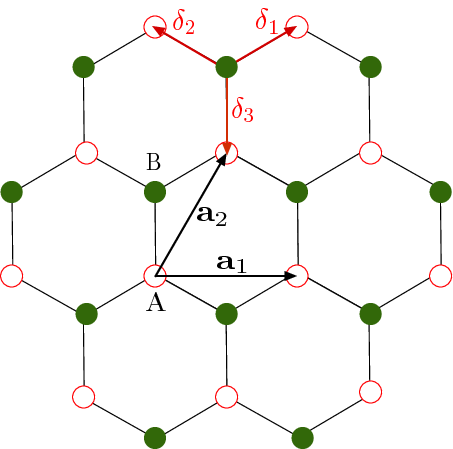
\includegraphics[width=0.5\linewidth]{images/HoneycombGreen}
	\caption{cite http://inspirehep.net/record/1256684/files/HoneycombGreen.png}
	\label{fig:honeycombgreen}
\end{figure}


where $a_{1,2} =a(\sqrt{3}/2),\pm1/2)$, and $\delta_3 =a(0,-1) $, where a is the lattice spacing as in fig~\ref{fig:honeycombgreen}. Notice there is no A to A and B to B terms, since these come from next nearest neighbor hopping at first order, and inversion symmetry enforces that they be equal. If they are the equal, it simply adds an identity piece to H(k).

Taking the Fourier transform, $c_r = \int_k \frac{dk^2}{(2\pi)^2}e^{-ikr} c_k$, each of the $+\delta$ terms simply contribute an $e^{\pm i k \cdot \delta}$ depending on whether there was a dagger or not. Now
\begin{align}
H(k)= 
\begin{pmatrix}
0 & h(k) \\
h^*(k) & 0
\end{pmatrix} \quad h(q) = \sum_i e^{-ik\delta_i} = e^{-ik_ya} + e^{ik_xa\sqrt{3}/2+ik_ya/2}+e^{-ik_xa\sqrt{3}/2+ik_ya/2} \\
h(q) = cos(k_ya)-i sin(k_ya) +(cos(k_ya/2)+i sin(k_ya/2))2cos(k_xa\sqrt{3}/2)
\end{align}
This means that $h_x(k) = cos(k_ya)+2cos(k_xa\sqrt{3}/2)cos(k_ya/2)$ and $h_y(k) = sin(k_ya)-2cos(k_xa\sqrt{3}/2)sin(k_ya/2)$. Notice $h_x(k) = 0$ when $k = \pm K = \frac{2\pi}{3a}(\pm1/\sqrt{3},-1)$, since $h_x(\pm K) = cos(\frac{2\pi}{3})+2cos(\pm\frac{\pi}{3})cos(\frac{\pi}{3})=0$, and $h_y(\pm K) = sin(\frac{2\pi}{3})-2cos(\pm\frac{\pi}{3})sin(\frac{\pi}{3})=0$.

This degeracy in general is protected by symmetries. First there is a time teversal symmetry T. In general, given any time dependent wave function, the time dependent pieces are a series of phases $e^{iEt/\hbar}$ onto time independent pieces. Changing the sign of t is equivalent here to complex conjugation, so T can be represented by the complex conjugation operator K. This representation is dependent on the basis. 
An important point here is that T is anti-unitary. In general under a symmetry S, any correlation function $|<Sa|Sb>| = |<a|b>|$. This means that $|<a|S^TS|b>| =|<a|b>|$ or $|<b|a>|$. Time reversal does the second. There is a simple theorem that says antiunitary symmetries are unitary symmetries with the complex conjugate operator. In this basis, creation and annihilation operators in real space map to real valued matricies, so K leaves them alone. It flips the sign of k, so it sends $c_k$ to $c_{-k}$. We can use the same basis of $\begin{pmatrix}
1 \\
0
\end{pmatrix} = c^{A\dag}_k|0>$ and  $\begin{pmatrix}
0 \\
1
\end{pmatrix} = c^{B\dag}_k|0>$
\begin{align}
THT^{-1}&=\int_{BZ}\frac{dk^2}{(2\pi)^2} 
\begin{pmatrix}
c^{A\dag}_k & c^{B\dag}_k
\end{pmatrix}
TH(k)T^{-1}
\begin{pmatrix}
c^{A}_k \\
c^{B}_k
\end{pmatrix}
 \\
&= \int_{BZ}\frac{dk^2}{(2\pi)^2} 
\begin{pmatrix}
c^{A\dag}_{k} & c^{B\dag}_{k}
\end{pmatrix}
KH(-k)K
\begin{pmatrix}
c^{A}_{k} \\
c^{B}_{k}
\end{pmatrix} = H
\end{align}

This implies $H^*(-k) = H(k)$. A symmetry can be thought of as both acting on H, and on k.

There is also an inversion symmetry P around the center of a unit cell which sends r to -r. Inversion P sends A sites to B sites, and B to A, while also flipping the sign of k. $\sigma_x$ flips the atoms, so P can be represented by $\sigma_x$. 

The Inversion operator flips the atoms and r coordinate of the real space c operators. This ends up sending $c^A_k = \int_r e^{-ikr}c^A_r$ to $c^B_{-k}$, and similarly with the rest. This has the effect of making the Hamiltonian
\begin{align}
PHP^{-1}&=\int_{BZ}\frac{dk^2}{(2\pi)^2} 
\begin{pmatrix}
c^{A\dag}_k & c^{B\dag}_k
\end{pmatrix}
PH(k)P^{-1}
\begin{pmatrix}
c^{A}_k \\
c^{B}_k
\end{pmatrix} \\
&= \int_{BZ}\frac{dk^2}{(2\pi)^2}
\begin{pmatrix}
c^{A\dag}_k & c^{B\dag}_k
\end{pmatrix}
\sigma_x H(-k) \sigma_x
\begin{pmatrix}
c^{A}_k \\
c^{B}_k
\end{pmatrix}
= H
\end{align}
Inversion makes sure $\sigma_x H(-k) \sigma_x =H(k)$. 

Together these constrain the Hamiltonian. By time reversal, $Kh_x(k) \sigma_xK = h_x(-k)\sigma_x$, which implies $h_x(-k)=h_x(k)$. Inversion makes $\sigma_x (h_x(k) \sigma_x) \sigma_x =h_x(-k)\sigma_x$ which implies the same thing. This means $h_x(k)$ is even in k. For $h_y(k)$, $K h_y(k) \sigma_y K =-h_y(-k)\sigma_y= h_y(k)\sigma_y$. This implies $h_y(k) = -h_y(-k)$. Inversion this time implies  $\sigma_x h_y(k) \sigma_y \sigma_x =-h_y(-k)\sigma_y=  h_y(k)\sigma_y$, which again is the same thing, making $h_y$ odd under k.

Now the important part. By time reversal, $Kh_z(k) \sigma_zK = h_z(-k)\sigma_z$, which implies $h_z(-k)=h_z(k)$. Inversion makes $\sigma_x (h_z(k) \sigma_z) \sigma_x = -h_z(-k)\sigma_z$, which implies $-h_z(-k)=h_z(k)$. Now we have $-h_z(-k)=h_z(-k)$, which implies $h_z(k)$ is zero!
This means that there is no $\sigma_z$ component. Then by squaring the H operator,
\begin{align}
H^2(k)= \sigma_x^2 h_x^2(k) + \sigma_y^2 h_y^2(k) \\
H^2(k)= h_x^2(k) + h_y^2(k) \\
E(k)=\pm\sqrt{h_x^2(k) + h_y^2(k)}
\end{align}.
Since there is no $\sigma_z$ piece, the only changes that could be added is parts to $h_x$ or $h_y$. Since around K or K' point there is $E(K+q)=\sqrt{q_x^2+q_y^2}$, all that can be done is add a constant, which would just shift the Dirac points, or add higher order pieces, which still go to zero. Now if one of the symmetries is broken, there can be d $\sigma_z$ pieces, which can gap out the system. There are topologically distinct ways to do this.

Consider a small constant $M\sigma_z$ term added to H(k), which can be done in real space by adding $Mc^{A\dagger}_rc^A_r - Mc^{B\dagger}_rc^B_r +h.c$ terms to the sum. This breaks inversion symmetry, and is physically making the atoms on the A site and B site different. In the limit of large M, this is basically binding all the atoms to one site. That is a model of a trivial insulator.

Haldane showed that there is a topologically nontrivial phase here, if time reversal is borken but not inversion. The intuition here being if there is a term that can be added is $h_z(k)\sigma_z$ where $h_z(k)=-h_z(-k)$ to preserve time reversal. In the limit that k is close to K
\begin{align}
H(q=(k-K))= \sigma_x h_x(q) + \sigma_y h_y(q) + \sigma_z h_z(q)\\
H(q)= c(\sigma_x q_x + \sigma_y  q_y) + \sigma_z h_z(q)
\end{align}
For some constant c. If $h_z\sigma_z$ is time reversal symmetric, the Hamiltonian near -K is known as well. 

 Haldane added next nearest neighbor hopping to another 6 sites, such that all lattice symmetries stayed. This adds a piece onto H(k) as follows:
\begin{align}
H_2(k) =  2t_2 cos(\phi)\sum_i cos(k \cdot b_i)  +2t_2 sin(\phi) \sum_i sin(k \cdot b_i)
\end{align} 
where $b_1 = \delta_2 - \delta_3$, $b_2 = \delta_3 - \delta_1$, and $b_3 = \delta_1-\delta_2.$ This makes $h_z(k=\pm K) = \mp 3\sqrt{3}t_2sin(\phi)$. In the limit of being close to K or -K, it is the fact that this gap flips sign at $\pm K$ that makes the topology nontrivial.

The berry curvature integral ends up taking the form
\begin{align}
n = \frac{1}{4\pi}\int_{BZ}dk^2 \partial_{k_x}\hat{h}(k) \times \partial_{k_y}\hat{h}(k) \cdot \hat{h}(k) \\
\hat{h}(k) = \vec{h}(k)/|\vec{h}(k)|
\end{align} 
This counts the number of times $\hat{h}(k)$ wraps around the unit sphere. Notice this is only defined when there is a gap. In the trivial phase, the z component of $\hat{h}(k)$ is always positive. That means $\hat{h}(k)$ can't possibly wrap around the sphere, so n would be 0. In this Haldane phase however, $\hat{h}(\pm K) = (0,0,\mp 1)$, and in fact wraps around the sphere exactly once. This phase actually exhibits a quantum Hall conductance of $\sigma_{xy}=e^2/h$. If this model is on a semi-infinite plane with an edge, there will be a single edge mode which carries this charge. Since this map can't go from n=1 to 0 continuously, the only way to change phases would be to close the gap, i.e. make $\hat{h}(k)$ ill-defined. This is the definition of a topological insulator! 

\subsection{Topological insulators with spin}

Now, this was just a toy model, in real life electrons have spin, and this changes things rather drastically. This thesis will go through a model by Kane and Mele~\cite{KaneMele2D1,KaneMele2D2}, which is written pedagogically in Fradkin's book~\cite{Fradkinbook}. Now there are two copies of the exact same model, one for spin up and one for spin down. A gap can be opened using spin-orbit interactions.

In the Haldane model, the Chern invariant ended up being how many times some vector $\hat{h}(k)$ wrapped around the sphere. Based on the sign difference of that at the old degenerate points the number of times it wrapped around the sphere could be deduced. The degenerate point $(k_1,k_2)=(\pi,\pi)$, where $k_i$ are reciprocal lattice vectors, was sent to K' under time reversal and inversion. Those relation put constraints on the Hamiltonian. When spin is involved, there can be a new topological invariant, which can be nonzero without time reversal breaking. 

With spinful electrons, the previous spinless model needs to be doubled, one for spin up and one for spin down. One can simply be the time reversal copy of the other. Now if the first has a Chern number of c, the second will have a Chern number of -c. The total charge conductance cancels out, but there is still a "spin current", since spin ups move in one direction and the spin downs move in the other. The topological invariant associated with this can again be found out by looking at old degenerate points and symmetry constraints.

Now the T operator is described. An interesting fact here is $T^2 =-1 $ for fermion systems. This can understood from CPT symmetry. In euclidean space CPT is just a 180 degree rotation. That squared then is a 360 rotation, which is +1 for bosons and -1 for fermions. If $(CP)^2=1$ and it is assumed these operators commute, then $T^2=-1$. T has to be real valued by the operation seen above, and has a piece that's $\tau_x$ or $\tau_y$, to switch spins. The $\tau_x$ would give the wrong $T^2$, so $T = i\tau_yK$, and $T^2 = i\tau_yi\tau_yK^2 = i^2 = -1$.

In 2+1 d spinful systems, there is whats called a Kramer's degeneracy protected by just time reversal. If $T|\phi>= e^{i\theta}|\phi>$, meaning $|\phi>$ is an eigenstate of T, then $TT|\phi> = T e^{i\theta}|\phi> = e^{-i\theta}T|\phi>=e^{-i\theta}e^{i\theta}|\phi>= |\phi>$ which implies $T^2=+1$. The contrapositive means if $T^2=-1$ on a state $|\phi>$then $|\phi>$ is not an eigenstate of T. Then if time reversal symmetry acts on a state $T|\phi_1(k)> = |\phi_2(-k)>$ and since H and T commute,
\begin{align}
TH|\phi_1(k)> = TE_1(k)|\phi_1(k)> = E_1(k)|\phi_2(-k)> \\
HT|\phi_1(k)> = H|\phi_2(-k)> = E_2(-k)|\phi_2(-k)> \\
E_1(k)=E_2(-k)
\end{align} 
So if there is a time reversal invariant point, i.e. $k=-k+G$ where G is a reciprocal lattice vector, there is a degeneracy. Again what matters is a different sign on the "mass" at degenerate points. Then the topological invariant is discovered by looking at these degenerate points, or the matrix given by $w_{ij}(k) = <\phi_i(-k)|T|\phi_j(k)>$, This is of interest when k is time reversal invariant. If it is assume for a moment that there are only 2 bands, this w is nonzero if $i\ne j$. It can be guessed that the sign of the gapping term would be given by the sign of $ \sqrt{\det{w(K)}}$. This is not just a simple $\pm1$, so interestingly enough the Pfaffian is used, which remember squares to the determinant. In the 2 x 2 case, it is just $M_{12}$. Define $\delta(k) = \sqrt{\det{w(K)}}/pfaff(w(K)) = \pm 1$, or in the 2 x 2 case = $\pm sgn(w_{12})$ This function is of great importance later in this thesis. One issue is the square root, which leaves the sign ambiguous. This is a continuous function however, and the sign differences at different invariant points is defined. In 2+1 d there are four time reversal invariant momenta $Q_i$, so let $(-1)^\nu = \prod_i \delta(Q_i)$. This ends up being gauge invariant and $\nu$ is a topological invariant that carries two values $0,1\mod 2$. It is called time reversal polarization.

This is called a $Z_2$ index. The reason why this is no longer Z classified is that there could be non spin conserving terms that are still time reversal invariant. If there is N chiral modes on the spin up sector, there will be N chiral modes on the spin down sector. If there are backscattering terms, there will be a scattering matrix. If  there is a state
\begin{align}
|\psi_{L}>=\sum_{i=1}^N \alpha_{i,L}|\psi_\uparrow^L>+\beta_{i,L} T|\psi_\uparrow^L> \\
|\psi_{R}>=\sum_{i=1}^N \alpha_{i,R}|\psi_\uparrow^R>+\beta_{i,R} T|\psi_\uparrow^R>  
\end{align}
with $\alpha$'s for the incoming modes and $\beta$'s for the outgoing. The scattering matrix goes as 

\begin{align}
\begin{pmatrix}
\vec{\beta}_L \\
\vec{\beta}_R
\end{pmatrix}
=
\begin{pmatrix}
r & t\\
t' & r'
\end{pmatrix}
\begin{pmatrix}
\vec{\alpha}_L \\
\vec{\alpha}_R
\end{pmatrix}
\end{align}
Now S has to be unitary since it is a change of basis from incoming to outgoing states. Time reversal will send outgoing to incoming and ect. S on the states now gives $ST^2\vec{\beta}^*=\vec{\alpha}^*$. The incoming $\beta$ states previously had no T's, and now there are two. If $vec{\beta}$ is solved for then $\vec{\beta}=T^2S^T\vec{\alpha}$. If $T^2=1$, this means $S=S^T$ together with $S^{-1}=S^\dag$. In this case if t=t'=0, that just requires r and r' to satisfy the same set of conditions. Yet if $T^2=-1$ that means S is antisymmetric. Then if t=t'=0 that means r and r' are antisymmetric and unitary. If N is odd, that means it there is an odd dimension antisymmetric matrix, which always has a zero eigenvalue. This is impossible for a unitary matrix. This means not only that t and t' are not zero, but that one mode must have perfect transmission. So this topological index simply measures the parity of the number of helical modes.

This generalizes to 3+1 d. There are 8 invariant points in 3+1, and $(-1)^{\nu_0} = \prod_i \delta_i$, and 3 more invariants $(-1)^{\nu_k} = \prod_i \delta_i$ where the sum is now just 4 points on the xy, yz, or zx planes of the Brillouin zone. This is just treated the 3d topological insulator as a 2d one in different projections. These three are called weak topological insulators and the sum over 8 is called a strong topological insulator, since it turns out to be robust to disorder.

Here is a brief summary of what was seen in this section. Topological insulators are band insulators that cannot be deformed into the atomic limit insulator without closing the gap. Two models of this were presented that exhibit the quantum Hall effect and the quantum spin Hall effect. The symmetries constrain the Hamiltonian to have a certain form, and if starting from a semi-metal, a gap can be opened in distinct ways. A topological index being zero does not mean the phase is trivial. For instance, the quantum spin Hall effect has trivial Chern number. Even if all the indecies known were zero there might be nonzero ones that haven not been thought of yet. A conventional TI has a set of symmetries, so far at minimum time reversal and charge conjugation.
 
This sums up an introduction to tools used in the two papers described in the rest of this thesis. Classical, integer quantum Hall, and then fractional quantum Hall were described. Following that the specifics of a $\nu=1/2$ state were seen. Then using conformal field theory these fractional excitations can be analyzed. These fractional states can be written in terms of electronic operators and vice versa. Now using this machinery a few questions can be addressed. First, since a Dirac mode can be split into Pfaffian modes, if a Dirac semimetal can be described using these Dirac modes, they can be split into Pfaffian modes. Perhaps backscattering Pfaffian modes can provide a new type of gapping. This will be explored first. Next, the Pfaffian state can live on the surface state of a topological insulator. This could be generalized to fractional topological insulators. That is the second publication. What follows is a mostly a direct exert from these publications~\cite{RazaSirotaTeo17,SahooSirotaChoTeo17}.
 



%\section{Background}
%
\subsection{Topological Phases of matter}
	To describe Topological phases we should first look at more familiar phases of matter. For example, let's look at fluids and solids. In a solid, the atoms become fixed in certain positions, called a lattice. These lattices can be described by a discrete translation symmetry. This means if you take your lattice, you can translate the entire structure a certain distance and direction, and you will end up exactly overlapping the original lattice. This translation symmetry is discrete since the vectors you can translate the lattice by are discrete. In reality though, these atoms wiggle in place so they won't be exactly where they should in the ideal crystal. You can introduce an observable to measure this. For instance you can take an atoms average distance away from the closest lattice site. In fact you can have this be a local measurement, by averaging them within some vicinity. You can understand the whole phase by only looking at some small part of it. We usually call this a local order parameter. You can even look at excitations of the solid using this local order parameter, in this case a wave would be a phonon. We would call that a quasiparticle. The idea is that the lattice is very close to the ground state, but in some vicinity there is an excitation. This does not imply you can remove it from the material, and hence it is not a true particle as known by the high energy community. 
	
	A fluid however is very different. If you take the fluid and translate it an arbitrary amount, the atoms on average will still look the same i.e. randomly organized. So we say that fluids have continuous translation symmetry. If we use the same local order parameter, when you melt a solid you would see a discontinuous jump as a function of temperature. This is what people usually understand phase transitions to be.	For different types of phases, you can typically see some local order parameter change discontinuously during a phase transition, but the trick is in knowing which order parameter to use. In a magnet you could average a few atoms magnetic field direction. If they are randomly aligned it will not be magnetic, but if there is some preferred direction it will have a macroscopic effect. There are many such local order parameters. You can think about either of these as a vector attached to each atom, but you can also think about it as a function from real space to some parameter space. There is no reason for the parameter space to be topologically the same as real space. For instance in the magnetic case, the direction matters but the magnitude does not, so you would have a map from $\mathbb{R}^3$ to $S_2$.
	
	This doesn't really mean anything deep since what we've talked about so far is all local, so the spaces topology, a global property is usually irrelevant. However this was found to actually be important since there are some phases described by global order parameters like the quantum hall effect. We can look at phase transitions in this picture as some global property changing discontinuously, like the band gap closing, or the existence of certain types of excitations. This is experimentally challenging, since you cannot measure what phase the material is in by doing an arbitrary local measurement. The information rather is stored across the entire material typically through quantum entanglement. Another added difficulty is these transitions are usually theoretically described at zero temperature, with the parameter being a function of some term in the Hamiltonian, which may or may not be physically realizable. There is a bulk boundary correspondence however, and you can say something about some global bulk properties by looking only at edge modes. 

\subsection{Toric Code}

	There are many ways to look at this topic, but perhaps the best thing to do is start off with a famous example, Kitaev's toric code. The basic idea is that with a certain Hamiltonian, the quasiparticle excitations will be exact energy eigenstates, and will be at exactly one lattice site. We will see how the excitations are entangled, how bulk boundary correspondence plays out, and how the quasiparticle content describes the phase completely.
	
	First we start with a square lattice where every link has a spin 1/2 on it, with the Hamiltonian 
	\[H = -\sum_pP_p-\sum_vV_v \]
	where the sum is over every plaquette p or every vertex v with 
	\[P_p = -\sum_p\sigma_z\,\quad V_v=\sum_v\sigma_x \] where these sums are over all the spins in any plaquette p, or vertex v, and the pauli matricies act on the 1x2 spin vector.
	\begin{figure}
		\centering
		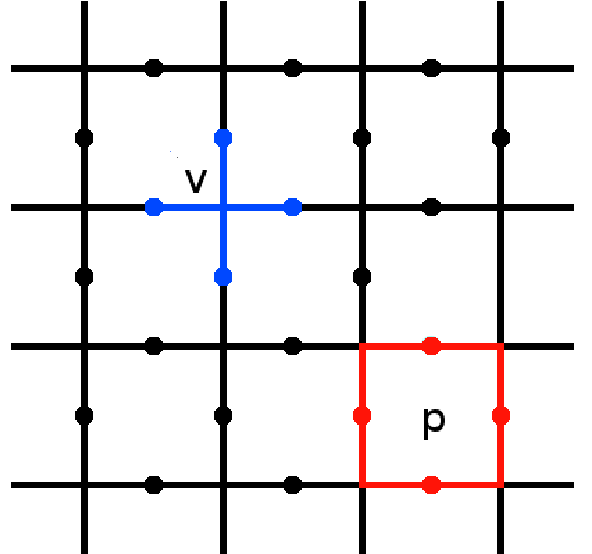
\includegraphics[width=0.5\linewidth]{ToricCodeLattice}
		\caption{Toric Code Lattice}
		\label{fig:toriccodelattice}
	\end{figure}
	
	The solution to this comes from the fact that the V and P operators are mutually commuting. $\sigma_z$ commutes with $\sigma_z$ so the P's commute, and $\sigma_x$ commutes with $\sigma_x$ so the V's commute. If a V and a P are far apart, they will act on different spins, so they will commute or they will share precisely 2 spins. If they share 2 spins a $\sigma_z$ commuting past a $\sigma_x$ will produce a sign, but that happens twice therefore all of these operators commute.
		
The second condition is that the operators only have eigenvalues of $\pm 1 $. This means that since each operator commutes with the Hamiltonian, every ground state must have P=V=1. This does not mean we've pinned
down the ground state yet. Now Euler's characteristic is $\#v-\#e+\#p = 0$ for any graph on a torus, where $\#v$ is the number of verticies, $\#p$ is the number of plaquettes and $\#e$ is the number of edges (links). That means that we have $ 2^{\#e} $ degrees of freedom since there is a spin on each edge but we have $2^(\#v+\#p)$ number of constraints, except that on a torus that overcounts by $2^2$, coming from the fact that $ \prod_v V_v =1 $ and $ \prod_p P_p =1 $ since every spin get's hit twice by a $ sigma_x $,squaring to 1, and twice by a $sigma_z$ term also squaring to 1. This means the total left over degrees of freedom is $ 2^(\#e-\#v-\#p+2) $ which is $2^(2)=4$. This means on a torus, even with those constrains, there is a ground state degeneracy of 4. This ground state degeneracy is a common thing in topological phases. 

The excitations are quiet simple, just have any V or P = -1. Now in order to flip the sign of a P term, we need to flip one of the spins on a vertex, but that spin is also attached to another vertex. This means flipping a spin creates two vertex excitations. If we try to flip another spin to undo one of them, we run into the same problem, we would add a sign to one vertex, and another too a second, which would only move the excitation around. In this sense, excitations can only be created in pairs, and can visualize a string of $\sigma_x$ operators connecting the two excitations. You can close the loop and annihilate the two excitations, leaving the state back in the ground state. Likewise, to flip the sign of the plaquette operator, you just need to apply a $sigma_z$, and the same string argument follows. If you apply a $sigma_y$ operator, you just get a pair of both the vertex and the plaquette excitations. The symbols for these quasiparticles are called e,m and $\psi$
\section{From Dirac semimetals to topological phases in three dimensions: a coupled wire construction}


%\definecolor{teal}{cmyk}{0.5,1,0,0}
%\definecolor{lightgreen}{cmyk}{0.25,0.25,0.4,0}


%\newcommand{\SPT}{\hyperlink{SPT}{SPT} }

%\begin{document}

%\title{Symmetry preserving gapping of Weyl and Dirac Semimetals}
%\title{\texorpdfstring{From Dirac semimetals to topological phases in three dimensions: \\ a coupled wire construction}{From Dirac semimetals to topological phases in three dimensions: a coupled wire construction}}
%\author{Syed Raza}
%\author{Alexander Sirota}
%\author{Jeffrey C. Y. Teo}\email{jteo@virginia.edu}
%\affiliation{Department of Physics, University of Virginia, Charlottesville VA 22904, USA}
%\date{\today}

\subsection{Introduction}\label{sec:introduction}
Dirac and Weyl semimetals are nodal electronic phases of matter in three spatial dimensions. Their low-energy emergent quasiparticle excitations are electronic Dirac~\cite{Dirac28} and Weyl~\cite{Weyl29} fermions. (Contemporary reviews in condensed electronic matter can be found in Ref.~\onlinecite{Ashvin_Weyl_review,TurnerVishwanath13,HasanXuBian15,RMP,Burkov16,JiaXuHasan16,ArmitageMeleVishwanath16,YanFelser17}.) They are three dimensional generalizations of the Dirac fermions that appear in two dimensional graphene~\cite{NetoGuineaPeresNovoselovGeim09} and the surface boundary of a topological insulator~\cite{HasanKane10,QiZhangreview11,HasanMoore11,RMP}. They follow massless quasi-relativistic linear dispersions near nodal points in the energy-momentum space close to the Fermi level. Contrary to accidental degeneracies which can be lifted by generic perturbations, these nodal points are protected by topologies or symmetries. 

A Weyl fermion is {\em chiral} and has a non-trivial winding of a pseudo-spin texture near the singular nodal point in energy-momentum space. This would associate to a non-conservative charge current under a parallel electric and magnetic field and is known as the Adler-Bell-Jackiw anomaly~\cite{Adler69,BellJackiw69}. Thus, in a true three dimensional lattice system, Weyl fermions must come in pairs~\cite{Nielsen_Ninomiya_1981,NielsenNinomiyaPLB1981,NielsenNinomiya83} so that the net chirality, and consequently the anomaly, cancels. Or otherwise, a three dimensional system of a single Weyl fermion must be holographically supported as the boundary of a topological insulator in four dimensions~\cite{ZhangHu01,BernevigChernHuToumbasZhang02,QiHughesZhang08}. On the other hand, a Dirac fermion in three dimensions consists of a pair of Weyl fermions with opposite chiralities. Without symmetries, it is not stable and can turn massive upon inter-Weyl-species coupling. With symmetries, a band crossing can be protected by the distinct symmetry quantum numbers the bands carry along a high symmetry axis. In this article, we focus on the fourfold degenerate Dirac nodal point protected by time-reversal and (screw) rotation symmetry.

In electronic systems, massless Dirac and Weyl fermions appear in gap-closing phase transitions between spin-orbit coupled topological insulators and normal insulators~\cite{Murakami2007}. When inversion or time-reversal symmetry is broken, nodal Weyl points can be separated in energy-momentum space. Such gapless electronic phases are contemporarily referred to as Weyl (semi)metals~\cite{WanVishwanathSavrasovPRB11,YangLuRan11,burkovBalenstPRL11,BurkovBalentsPRB11}. Their boundary surfaces support open Fermi arcs~\cite{WanVishwanathSavrasovPRB11} that connect surface-projected Weyl nodes. Weyl (semi)metals also exhibit exotic transport properties, such as negative magneto-resistance, non-local transport, chiral magnetic effect, and chiral vortical effect~\cite{Burkov_Weyl_electromagnetic_2012,Hosur_Weyl_develop,Lu_anomaly_Weyl_2013,SonSpivak13,Sid_anomaly_Weyl,Marcel_Weyl_response}. There have been numerous first principle calculations~\cite{WengXiZhong16} on proposed materials such as the non-centrosymmetric (La/Lu)Bi$_{1-x}$Sb$_x$Te$_3$~\cite{LiuVanderbilt14}, the TlBiSe$_2$ family~\cite{SinghSharmaLinHasanPrasadBansil12}, the TaAs family~\cite{WengBernevigDai2015,HuangXuZahidTaAs2015}, trigonal Se/Te~\cite{HirayamaOkugawaIshibashiMurakamiMiyake15} and the HgTe class~\cite{RuanXing16}, as well as the time-reversal breaking pyrochlore iridates \cite{WanVishwanathSavrasovPRB11,witczak_kim_weyl_2012,chen_hermele_weyl}, magnetically doped topological and trivial insulator multilayers \cite{burkovBalenstPRL11}, HgCr$_2$Se$_4$~\cite{XuWengWangDaiFang11} and Hg$_{1-x-y}$Cd$_x$Mn$_y$Te~\cite{BulmashLiuQi14}. At the same time, there have also been abundant experimental observations in bulk and surface energy spectra~\cite{HasanXuBelopolskiHuang17} as well as transport~\cite{WangLinWangYuLiao17}. Angle-resolved photoemission spectroscopy (\hypertarget{ARPES}{ARPES}) showed bulk Weyl spectra and surface Fermi arcs in TaAs~\cite{Xu_Weyl_2015_first,Weyl_discovery_TaAs,YangLiuChenTaAs2015,TaAs_Weyl_obeservationDing,BelopolskiZahid16} as well as similar materials such as NbAs, NbP and TaP~\cite{XuNbAs15,LiuChen16}. Other materials such as Ag$_3$BO$_3$, TlTe$_2$O$_6$ and Ag$_2$Se~\cite{ChangHasan16} were observed to host pinned Weyl nodes at high symmetry points. %theory pinned along screw axis {TsirkinSouzaVanderbilt17}
Negative magneto-resistance was reported in TaAs~\cite{Huang_Weyl_2015,Zhang_anomaly_Weyl_2015} as a suggestive signature of the Adler-Bell-Jackiw anomaly. Similar properties were also observed in TaP~\cite{HuMaoTaP17}, NbP and NbAs~\cite{CorinnaNiemannFelserNbP17,LiXuNbAsNbP17,GoothNielschNbP17}, although not without controversies~\cite{SudeshPatnaikNbP17}. 

Weyl points with opposite chiralities cannot be separated in energy-momentum space when both inversion and time reversal symmetries are present. Massless Dirac fermions appear between gap-closing phase transitions between topological and trivial (crystalline) insulators, such as Bi$_{1-x}$Sb$_x$~\cite{TeoFuKane08} and Pb$_{1-x}$Sn$_x$Te~\cite{Hsieh:2012fk}. Critical Dirac (semi)metals were investigated for example in the tunable TlBiSe$_{2-x}$S$_x$~\cite{SatoTakahashi11,SoumaAndo12,XuCavaHasan11}, Bi$_{2−x}$In$_x$Se$_3$~\cite{BrahlekSeongshik12,WuArmitage13} and Hg$_{1-x}$Cd$_x$Te~\cite{OrlitaPotemski14}, as well as the charge balanced BaAgBi~\cite{DuWanXYBi15}, PtBi$_2$, SrSn$_2$As$_2$~\cite{GibsonCava15} and ZrTe$_5$~\cite{LiVallaZrTe516} whose natural states are believed to be close to a topological critical transition. A Dirac (semi)metallic phase can be stablized when the Dirac band crossing is secured along a high symmetry axis and the two crossing bands carry distinct irreducible representations. Theoretical studies include the diamond-structured $\beta$-crystobalite BiO$_2$ family~\cite{BiO3_Dirac_semimetal} No.~227, Fd3m), the orthorhombic body-centered BiZnSiO$_4$ family~\cite{SteinbergYoungZaheerKaneMeleRappe14} (space group No.~74, Imma), the tetragonal Cd$_3$As$_2$~\cite{wangCd3As2PRB13} (space group No.~142, I4$_1$/acd), the hexagonal Na$_3$Bi family~\cite{Dai_predition_Na3Bi}, as well as the filling-enforced non-symmorphic Dirac semimetals~\cite{KonigMermin97,ParameswaranTurnerArovasVishwanath13,WatanabePoVishwanathZaletel15,ChenKimKee16,WatanabePoZaletelVishwanath16} such as the hexagonal TlMo$_3$Te$_3$ family~\cite{GibsonCava15} (space group No.~176, P6$_3$/m), the monoclinic Ca$_2$Pt$_2$Ga (space group No.~15, C2/c), AgF$_2$, Ca$_2$InOsO$_6$ (space group No.~14, P2$_1$/n), and the orthorhombic CsHg$_2$ (space group No.~74, Imma)~\cite{ChenPoNeatonVishwanath16}. At the same time, there are numerous experimental confirmations. They include \ARPES observations on Cd$_2$As$_3$~\cite{Cd3As2Chen2014,neupaneDiracHasan,borisenkoPRLCd3As2}, Na$_3$Bi~\cite{Liu21022014,Xu18122014} and ZrTe$_5$~\cite{LiVallaZrTe516}; scanning tunneling microscopy in Cd$_2$As$_3$~\cite{Yazdani_CdAs}; magneto-transport in Bi$_{1-x}$Sb$_x$~\cite{KimLiBiSb13}, Cd$_2$As$_3$~\cite{liangOngTransportCd3As2,HeLi14,XiangChen15,FengLuCd3As215,LiYuCd3As215,LiWangCd3As216,GuoLeeCd2As316,ZhangXiuCd3As217}, Na$_3$Bi~\cite{Xu18122014,XiongOng15}, ZrTe$_5$~\cite{ZhengMingliangZrTe514,LiVallaZrTe516,LiangOngHallZrTe516,YuanXiuZrTe516}, HfTe$_5$~\cite{WangWangHfTe516} and PtBi$_2$~\cite{GaoTianPtBi217}; magneto-optics~\cite{AkrapOrlitaCd2As316} and anomalous Nernst effect~\cite{LiangOngNernstCd3As217} in Cd$_2$As$_3$, and many more. However, there are also contradicting pieces of evidence, especially in ZrTe$_5$ and HfTe$_5$ that suggest a bulk band gap~\cite{WengDaiFangZrTe514,LiXingZrTe516,WuPanZrTe516,MoreschiniGrioniZrTe516,ManzoniCrepaldiZrTe516,ManzoniParmigianiZrTe517,FanZhouZrTe517}.
%Cd3As2
%SdH\cite{HeLi14,XiangChen15,GuoLeeCd2As316} negative magnetoresistance\cite{liangOngTransportCd3As2} anomalous Nernst effect\cite{LiangOngNernstCd3As217} magneto-optics\cite{AkrapOrlitaCd2As316}
%Na3Bi
%negative magnetoresistance\cite{Xu18122014,XiongOng15}
%ZrTe5
%negative magnetoresistance\cite{ZhengMingliangZrTe514,LiVallaZrTe516} anomalous Hall\cite{LiangOngHallZrTe516}
%HfTe5
%negative magnetoresistance\cite{WangWangHfTe516}
%PtBi2
%magnetoresistance\cite{GaoTianPtBi217}

\begin{figure}[htbp]
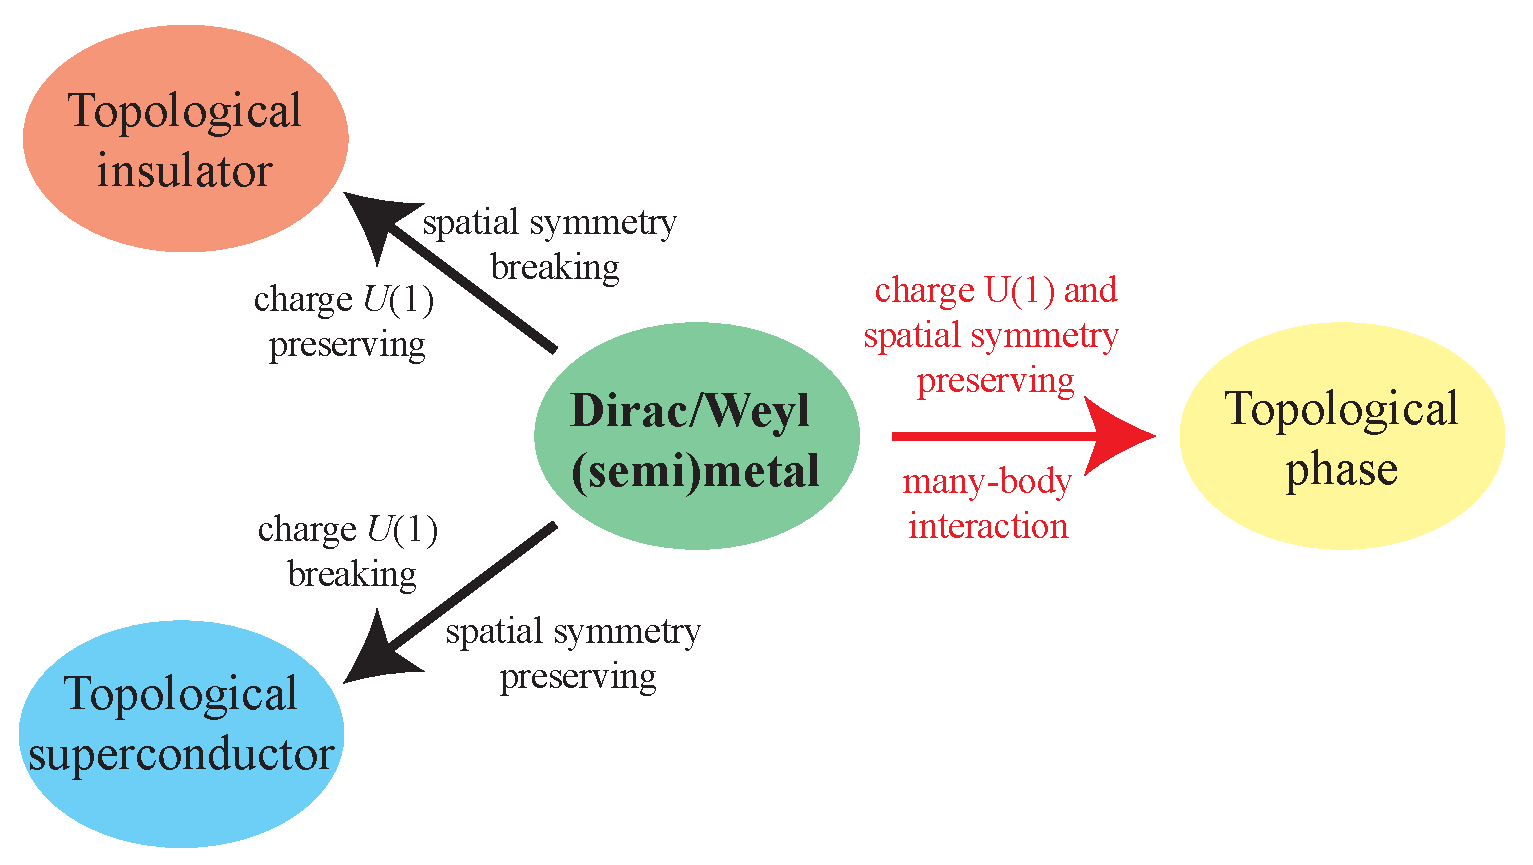
\includegraphics[width=0.45\textwidth]{intro}
\caption{Symmetry breaking single-body gapping versus symmetry preserving many-body gapping of a Dirac/Weyl (semi)metal.}\label{fig:intro}
\end{figure}

Dirac/Weyl (semi)metals are the origins of a wide variety of topological phases in three dimensions (see figure~\ref{fig:intro}). By introducing a spatial or charge $U(1)$ symmetry-breaking single-body mass, they can be turned into a topological insulator or superconductor. The focus of this manuscript is on symmetry-preserving many-body gapping interactions. The resulting insulating topological phase can carry long-range entanglement and a non-trivial topological order. Similar phenomena were theoretically studied on the Dirac surface state of a topological insulator~\cite{WangPotterSenthilgapTI13,MetlitskiKaneFisher13b,ChenFidkowskiVishwanath14,BondersonNayakQi13} and the Majorana surface state of a topological superconductor~\cite{LukaszChenVishwanath,MetlitskiFidkowskiChenVishwanath14}, where symmetry-preserving many-body gapping interactions are possible and lead to non-trivial surface topological orders that support anyonic quasiparticle excitations.

Symmetry-preserving gapping interactions cannot be studied using a single-body mean-field theory. This is because the Dirac/Weyl (semi)metallic phase is protected by symmetries in the single-body setting and any mean-field model with an excitation energy gap must therefore break the symmetry either explicitly or spontaneously. The coupled wire construction can serve as a powerful tool in building an exactly-solvable interacting model and understanding many-body topological phases of this sort. The construction involves a highly anisotropic approximation where the electronic degrees of freedom are confined along an array of continuous one-dimensional wires. Inspired by sliding Luttinger liquids~\cite{OHernLubenskyToner99,EmeryFradkinKivelsonLubensky00,VishwanathCarpentier01,SondhiYang01,MukhopadhyayKaneLubensky01}, the coupled wire construction was pioneered by Kane, Mukhopadhyay and Lubensky~\cite{KaneMukhopadhyayLubensky02} in the study of Laughlin~\cite{Laughlin83} and Haldane-Halperin hierarchy~\cite{Haldane83,Halperin84} fractional quantum Hall states. Later, this theoretical technique was applied in more general fractional quantum Hall states~\cite{TeoKaneCouplewires,KlinovajaLoss14,MengStanoKlinovajaLoss14,SagiOregSternHalperin15,KaneSternHalperin17}, anyon models~\cite{OregSelaStern14,StoudenmireClarkeMongAlicea15}, spin liquids~\cite{MengNeupertGreiterThomale15,GorohovskyPereiraSela15}, (fractional) topological insulators~\cite{NeupertChamonMudryThomale14,KlinovajaTserkovnyak14,SagiOreg14,SagiOreg15,SantosHuangGefenGutman15} and superconductors~\cite{mongg2,SeroussiBergOreg14}, as well as the exploration of symmetries and dualities~\cite{MrossAliceaMotrunich16,MrossAliceaMotrunich17}. Moreover, coupled wire construction has already been used to investigate three dimensional fractional topological phases~\cite{Meng15} and Weyl (semi)metal~\cite{Vazifeh13} even in the strongly-correlated fractional setting~\cite{MengGrushinShtengelBardarson16}.

The microscopic symmetry-preserving many-body interactions in the Dirac surface state on a topological insulator was discussed by Mross, Essin and Alicea in Ref.\onlinecite{MrossEssinAlicea15}. They mimicked the surface Dirac modes using a coupled wire model and proposed explicit symmetric many-body interactions that lead to a variation of gapped and gapless surface states. Motivated by this and also using a coupled wire construction, the microscopic symmetry-preserving many-body gapping of the Majorana topological superconducting surface state was studied by one of us in Ref.\onlinecite{SahooZhangTeo15}. 

In this article, we focus on (i) a coupled wire realization of a Dirac/Weyl (semi)metallic phase protected by antiferromagnetic time-reversal and screw twofold rotation symmetries, (ii) a set of exactly-solvable inter-wire many-body interactions that introduces a finite excitation energy gap while preserving the symmetries, and (iii) an interaction-enabled (semi)metallic electronic phase which is otherwise forbidden by symmetries in the single-body setting.

\subsubsection{Summary of results}\label{sec:introsummary}

We now highlight our results. The first part of this article addresses a mapping between the isotropic massless Dirac fermion in the continuum limit and an anisotropic coupled wire model where the effective low-energy degrees of freedom are confined along a discrete array of 1D continuous wires. We begin with a minimal Dirac (semi)metal equipped with time-reversal and (screw) $\mathcal{C}_2$ rotation symmetries. The mapping to a coupled wire model is achieved by first introducing vortices that break the symmetries microscopically. These vortices are topological line defects that involve spatial winding of symmetry-breaking Dirac mass parameters. Consequently, these vortices host chiral Dirac electronic channels, each of which corresponds to a gapless quasi-1D system where electronic quasiparticles can only propagate in a single direction along the channel and are localized along the perpendiculars. 

When assembled together onto a vortex lattice, the system recovers the screw $\mathcal{C}_2$ rotation symmetry as well as a set of emergent antiferromagnetic symmetries, which are combinations of the broken time-reversal and half-translations. Upon nearest-wire single-body electron backscattering, the electronic band structure disperses linearly and mirrors that of the continuous isotropic Dirac parent state. A symmetry-protected massless Dirac fermion (equivalently a pair of Weyl fermions with opposite chiralities) emerges and captures the low-energy long length scale electronic properties.

This mapping can be qualitatively understood as a coarse-graining procedure where high-energy microscopic electronic degrees of freedom are integrated out. The procedure can be repeated indefinitely and resembles a real-space renormalization. For example, the gapless Dirac electronic structure of the coupled wire model can acquire a finite mass by symmetry-breaking dimerizations. These dimerizations can be arranged in a topological manner that spatially wind non-trivially around a collective vortex. These second-stage vorticies can subsequently be assembled into an array similar to the previous construction except now with a longer lattice constant. The system again recovers a massless Dirac spectrum under inter-vortex electron tunneling in low-energy and long length scale. The mapping therefore establishes an equivalence between the continuous isotropic massless Dirac fermion and the semi-discrete anisotropic coupled Dirac wire model.

The second part of this article addresses non-trivial symmetry-preserving many-body interacting effects beyond the single-body mean-field paradigm. We begin with the anisotropic array of chiral Dirac wires that constitutes a Dirac (semi)metal protected by antiferromagnetic time-reversal (\AFTR) and (screw) $\mathcal{C}_2$ rotation symmetries. We consider an exactly-solvable model of symmetry-preserving inter-wire many-body backscattering interactions. This model is inspired by and can be regarded as a layered version of the symmetric massive interacting surface state of a topological insulator. It is based on a {\em fractionalization} scheme that divides a single chiral Dirac channel into a decoupled pair of identical chiral ``Pfaffian" channels. Each of these fractional channels carries half of the degrees of freedom of the original Dirac wire. For instance, the fractionalization splits the electric and thermal currents exactly in half. %The bipartition is stabilized by many-body interactions and cannot be realized in any single-body mean-field description. 
It leads to the appearance of fractional quasiparticle excitations. For example, a chiral Pfaffian channel also runs along the 1D edge of the particle-hole symmetric Pfaffian fractional quantum Hall state~\cite{Son15,BarkeshliMulliganFisher15,WangSenthil16}, and supports charge $e/4$ Ising and $e/2$ semionic primary fields.

We consider an explicit combination of many-body interwire backscattering interactions that stabilize the fractionalization. Similar coupled wire constructions were applied in the literature to describe topological insulator's surface state~\cite{MrossEssinAlicea15} and $\nu=1/2$ fractional quantum Hall states~\cite{TeoKaneCouplewires,KaneSternHalperin17}. They are higher dimensional analogues of the Affleck-Kennedy-Lieb-Tasaki (AKLT) spin chain model~\cite{AKLT1,AKLT2}. The pair of chiral Pfaffian channels along each wire is backscattered in opposite directions to neighboring wires by the interaction. As a result of this dimerization of fractional degrees of freedom, the model acquires a finite excitation energy gap and at the same time preserves the relevant symmetries.

The coupled wire construction also suggests new {\em interaction-enabled topological (semi)metals}. In the single-body regime, an (antiferromagnetic) time-reversal symmetric Weyl (semi)metal realizable on a three dimensional lattice has a minimum of four momentum-space-separated Weyl nodes. The many-body interacting wire model can be turned into a gapless system where all low-energy degrees of freedom are electronic and are freely described in the single-body non-interacting setting by two and only two separated Weyl nodes. Although the model is antiferromagnetic, we conjecture that similar anomalous Weyl (semi)metal can be enabled by interaction while preserving local time-reversal.

The paper is organized as follows. In section~\ref{sec:DiracSemimetal}, we construct a single-body coupled wire model of a Dirac/Weyl (semi)metal equipped with two emergent antiferromagnetic time-reversal (\AFTR) axes and a (screw) $\mathcal{C}_2$ rotation symmetry. In section~\ref{sec:anomaly}, we establish the equivalence between the isotropic continuum limit and the anisotropic coupled wire limit by a coarse-graining mapping. We also discuss the anomalous aspects of the pair of Weylrmions and different resolutions to the anomaly. Then we describe the gapless surface states of the coupled wire model. \AFTR breaking and preserving surfaces are considered separately in section~\ref{sec:fermiarcAFTRbreaking} and \ref{sec:fermiarcAFTRpreserving} respectively.

In section~\ref{sec:interaction}, we move on to the effect of symmetry-preserving many-body interactions. The fractionalization of a chiral Dirac channel is explained in section~\ref{sec:gluing}, where we review the content of the fractional Pfaffian conformal field theory and establish the decomposition $\mathrm{Dirac}\approx\mathrm{Pfaffian}\otimes\mathrm{Pfaffian}$ through bosonization techniques. The splitting of a Dirac channel is summarized in figure~\ref{fig:fractionalization}. In section~\ref{sec:interactionmodels}, we explicitly construct an exactly-solvable interacting coupled wire model that introduces a finite excitation energy gap to the Dirac system while preserving the relevant symmetries. The many-body interwire backscattering interactions are summarized in figure~\ref{fig:gappinginteraction}. In section~\ref{sec:AFMstablization}, we discuss a plausible stabilization mechanism of the desired interactions through an antiferromagnetic order. In section~\ref{sec:intenable}, we discuss a variation of the model that enables an anomalous topological (semi)metal with two Weyl nodes through interaction. In section~\ref{sec:fracsurface}, we elaborate on the gapless surface states of these new interacting phases.




\subsection{Coupled wire construction of a Dirac semimetal}\label{sec:DiracSemimetal}
We begin with a Dirac semimetal in three dimensions. It consists of a pair of massless Weyl fermions with opposite chiralities. In this article we do not distinguish between a Dirac and a Weyl semimetal. This is because the fermion doubling theorem~\cite{Nielsen_Ninomiya_1981,NielsenNinomiyaPLB1981,NielsenNinomiya83} and the absence of the Adler-Bell-Jackiw anomaly~\cite{Adler69,BellJackiw69} require Weyl fermions to always come in pairs in a three dimensional lattice system. A Weyl semimetal therefore carries the same low energy degrees of freedom as a Dirac semimetal. We refer to the case when the pair of Weyl fermions are separated in momentum space as a translation symmetry protected Dirac semimetal. Here, we assume the simplest case where the two Weyl fermions overlap in energy-momentum space. Its low-energy band Hamiltonian takes the spin-orbit coupled form \begin{align}H^0_{\mathrm{Dirac}}({\bf k})=\hbar v{\bf k}\cdot\vec{s}\mu_z\label{DiracHam0}\end{align} where $\vec{s}=(s_x,s_y,s_z)$ are the spin-$1/2$ Pauli matrices, and $\mu_z=\pm1$ indexes the two Weyl fermions.

\begin{figure}[htbp]
\centering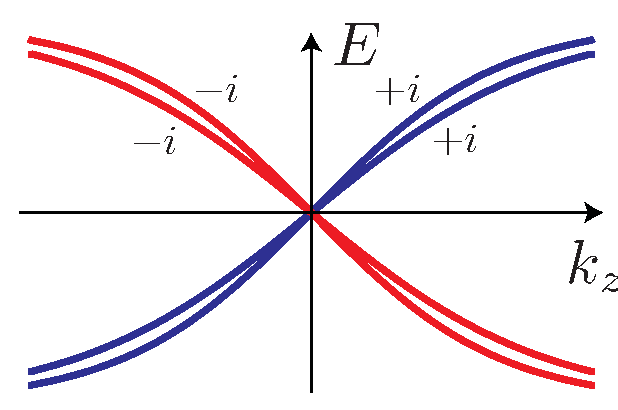
\includegraphics[width=0.25\textwidth]{Diracbands}
\caption{The two pairs of counter-propagating Dirac bands along the $k_z$-axis distinguished by eigenvalues of $C_2=\pm i$.}\label{fig:Diracbands}
\end{figure}

Normally the masslessness of the Dirac system is protected by a set of symmetries. Here, we assume the time reversal (TR) $\mathcal{T}$, which is represented in the single-body picture by the spinful operator $\hat{T}=is_y\mathcal{K}$ where $\mathcal{K}$ is the complex conjugation operator, and a twofold rotation $C_2$ about the $z$-axis. In the case when $\mu_z$ has a non-local origin such as sublattice or orbital, it can enter the rotation operator. We assume $\mathcal{C}_2$ is represented in the single-body picture by $\hat{C}_2=is_z\mu_z$. It squares to minus one in agreement with the fermionic statistics, and commutes with the local time reversal operator. In momentum space, $\mathcal{T}$ flips ${\bf k}\to-{\bf k}$ while $C_2$ rotates $(k_x,k_y,k_z)\to(-k_x,-k_y,k_z)$. The band Hamiltonian \eqref{DiracHam0} shares simultaneous eigenstates with $C_2$ along the $k_z$-axis. The two forward moving bands have $C_2$ eigenvalues $+i$ while the two backward moving ones have $C_2$ eigenvalues $-i$ (see figure~\ref{fig:Diracbands}). Therefore the band crossing is $C_2$-protected while the fourfold degeneracy is pinned at ${\bf k}=0$ because of time reversal symmetry. Noticing that each of the $C_2=\pm i$ sector along the $k_z$-axis is chiral (i.e.~consisting of a single propagating direction), it violates the fermion doubling theorem~\cite{Nielsen_Ninomiya_1981,NielsenNinomiyaPLB1981} and is anomalous. This can be resolved by assuming the $C_2$ symmetry is actually a non-symmorphic screw rotation in the microscopic lattice limit and squares to a primitive lattice translation in $z$. $k_z$ is now periodically defined (up to $2\pi/a$) and the two $C_2$ eigen-sectors wraps onto each other after each period. Focusing on the continuum limit where $k_z$ is small (when compared with $2\pi/a$), $C_2^2=-e^{ik_za}\approx-1$ and the $C_2$ symmetry behaves asymptotically as a proper rotation.

The primary focus of this article is to explore symmetry preserving/enabled interacting topological states that originate from the massless Dirac system. Contrary to its robustness in the single-body non-interacting picture, we show that the 3D Dirac fermion can acquire a many-body mass gap without violating the set of symmetries. To illustrate this, we first make use of the fact that the Dirac system can be turned massive by breaking symmetries. Symmetry breaking inter-valley scatterings introduce two coexisting mass terms \begin{align}H_{\mathrm{Dirac}}({\bf k},{\bf r})=H_{\mathrm{Dirac}}^0({\bf k})+m_x({\bf r})\mu_x+m_y({\bf r})\mu_y\label{DiracHam}\end{align} where $m_x$ (or $m_y$) preserves (resp.~breaks) time reversal, and both of them violate $C_2$. We allow slow spatial modulation of the mass parameters, which can be grouped into a single complex parameter $m({\bf r})=m_x({\bf r})+im_y({\bf r})$, and to be precise, momentum ${\bf k}$ should be taken as a differential operator $-i\nabla_{\bf r}$ when translation symmetry is broken. Non-trivial spatial windings of the symmetry breaking mass parameters give rise to topological line defects or vortices that host protected low-energy electronic degrees of freedom. Proliferation of interacting vortices then provides a theoretical path to multiple massive/massless topological phases while restoring and modifying the original symmetries as they emerge in the low-energy long-length scale effective theory.

\begin{figure}[htbp]
\centering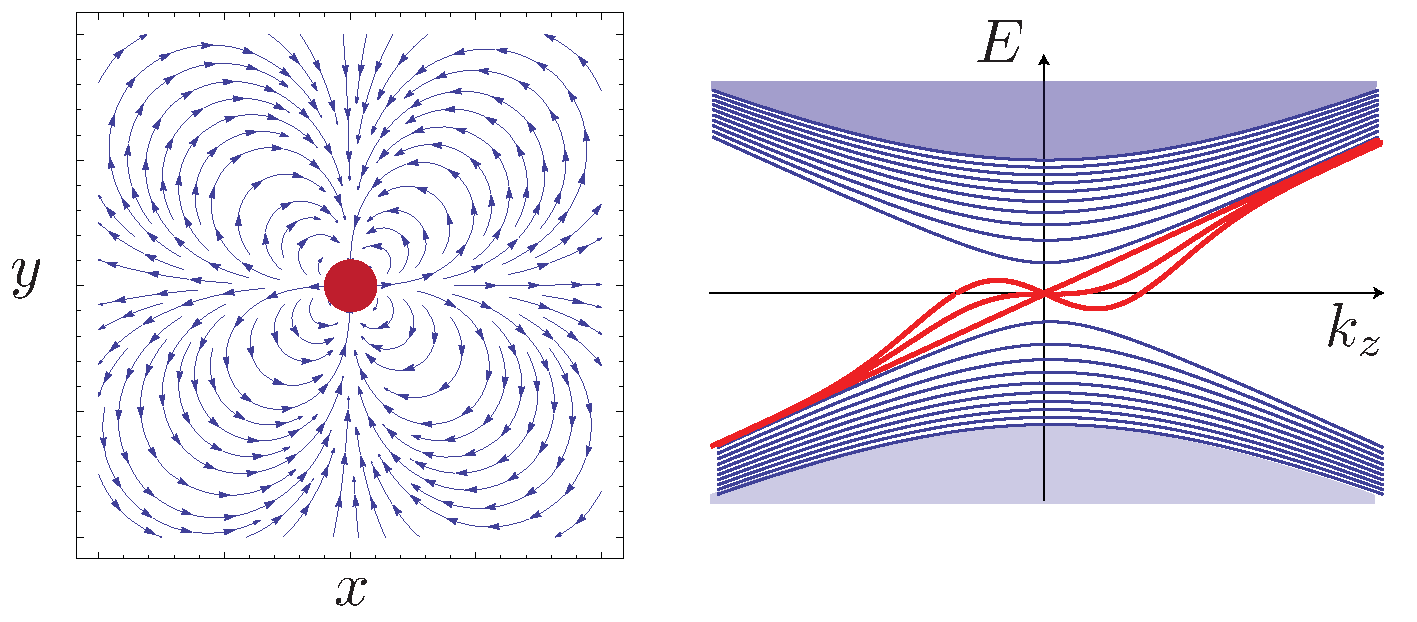
\includegraphics[width=0.4\textwidth]{Diracstring}
\caption{Dirac string. (Left) Spatial winding of mass parameters around a Dirac string going out of the paper represented by the center red dot. Stream lines represent the vector field ${\bf m}({\bf r})=(m_x({\bf r}),m_y({\bf r}))$. (Right) Energy spectrum of chiral Dirac fermions. Blue bands represent bulk continuum. Red bands correspond to chiral Dirac fermions localized along the string.}\label{fig:Diracstring}
\end{figure}

A topological line defect is a vortex string of the mass parameter in three dimensions where the complex phase of $m({\bf r})=|m({\bf r})|e^{i\varphi({\bf r})}$ winds non-trivially around the string. The left diagram in figure~\ref{fig:Diracstring} shows the spatial modulation of $\varphi({\bf r})$ along the $xy$ cross-sectional plane normal to a topological line defect, which runs along the $z$ axis. In this example, the complex phase $\varphi({\bf r})$ winds by $6\pi$ around the line defect (represented by the red dot at the origin). The winding number of the complex phase in general can be evaluated by the line integral \begin{align}c=\frac{1}{2\pi}\oint_\mathcal{C}d\varphi({\bf r})=\frac{1}{2\pi i}\oint_\mathcal{C}\frac{\nabla_{\bf r}m({\bf r})}{m({\bf r})}\cdot d{\bf r}\label{winding}\end{align} where $\mathcal{C}$ is a (righthanded) closed path that runs once around the (oriented) line defect. Eq.\eqref{winding} is always an integer given that the mass parameter $m({\bf r})$ is non-vanishing along $\mathcal{C}$.

Massless chiral Dirac fermions run along these topological line defects~\cite{TeoKane}.

We begin with the Dirac Hamiltonian \eqref{DiracHam} where the mass term winds around a vortex and as a consequence, it hosts a chiral Dirac channel along the vortex (also see figure~\ref{fig:Diracstring}). Here we will demonstrate an example of a simple vortex, and show that there is a chiral Dirac zero mode. In general, the correspondence between the number of protected chiral Dirac channels and the vortex winding is a special case of the Atiyah-Singer Index theorem~\cite{AtiyahSinger63} and falls in the physical classification of topological defects~\cite{TeoKane}.

First, say we start with the Hamiltonian from \eqref{DiracHam}. Then for simplicity we consider the particular Dirac mass $m({\bf r})=m_x({\bf r})+im_y({\bf r})=|m|e^{i\theta}$ that constitute a vortex along the $z$-axis, where $\theta$ is the polar angle on the $xy$-plane. By replacing $k_{x,y}\leftrightarrow-i\partial_{x,y}$, \eqref{DiracHam} becomes \begin{align}H({\bf r})=&\hbar v(-i\partial_xs_x-i\partial_ys_y+k_zs_z)\mu_z\nonumber\\&\;+|m|\cos\theta\mu_x+|m|\sin\theta\mu_y\label{DiracHamapp}\end{align} where $k_z$ is still a good quantum number because translation in $z$ is still preserved. The Hamiltonian can be transformed under a new basis into \begin{align}H'=UHU^{-1}=\left(\begin{smallmatrix}-\hbar vk_z&D\\D^\dagger&\hbar vk_z\end{smallmatrix}\right),\quad U =\left(\begin{smallmatrix}0&1&0&0\\0&0&1&0\\1&0&0&0\\0&0&0&1\end{smallmatrix}\right)\end{align} where the Dirac operator occupying the off-diagonal blocks is \begin{align}D^\dagger &=\left(\begin{smallmatrix}-2i\hbar v\partial_w&|m|e^{-i\theta}\\|m|e^{i\theta}&2i\hbar v \partial_{\bar{w}}\end{smallmatrix}\right)\nonumber\\&=e^{-i\theta\sigma_z}\left(\begin{smallmatrix}-i\hbar v(\partial_r-i \partial_\theta/r)&|m|\\|m|&i\hbar v(\partial_r+i\partial_\theta/r)\end{smallmatrix}\right)\end{align} where $w=x+iy=re^{i\theta}$ and $\sigma_z=\mathrm{diag}(1,-1)$. 

Now we separate the Hamiltonian \begin{align}H'(k_z)=\hbar vk_z\Gamma_5+\left(\begin{smallmatrix}0&D\\D^\dagger&0\end{smallmatrix}\right).\end{align} where $\Gamma_5=\mathrm{diag}(-\openone_2,\openone_2)$. We note that the zero momentum sector $H'(k_z=0)$ has a chiral symmetry since it anticommutes with with $\Gamma_5$, and it reduces to the Jackiw-Rossi vortex problem in two-dimensions~\cite{JackiwRossi81}. The Dirac operator $D^\dagger$ has only one normalizable zero mode $u_0(r)\propto e^{-|m|r/\hbar v}(e^{i\pi/4}, e^{-i\pi/4})^T$, while its conjugate $D$ has none. $H'(k_z=0)$ therefore has a zero eigenvector of $\psi_0(r)=(u_0(r),0)^T$, which is also an eigenvector of $\Gamma_5$. In the full Hamiltonian, the zero mode $\psi_0(r)$ has energy $-\hbar vk_z$ and corresponds a single mid-gap chiral Dirac channel.

When focusing at $k_z=0$, the differential operator \eqref{DiracHam} with a vortex along the $z$-axis is identical to the 2D Jackiw-Rossi model~\cite{JackiwRossi81} with chiral symmetry $\gamma_5=s_z\mu_z$. Each zero energy mode corresponds to a massless chiral Dirac fermion with positive or negative group velocity in $z$ depending on the sign of its $\gamma_5$ eigenvalue. These quasi-one dimensional low-energy electronic modes are similar to those that run along the edge of 2D Landau levels and Chern insulators, except they are now embedded in three dimensions. Their wave functions extend along the defect string direction but are localized and exponentially decay away from the defect line. Moreover, such an electronic channel is chiral in the sense that there is only a single propagating direction. The energy spectrum of the topological line defect (for the example with winding number $c=3$) is shown in the right diagram of figure~\ref{fig:Diracstring}, in which, there are three chiral bands (red curves) inside the bulk energy gap representing the 3 chiral Dirac electrons. As a consequence of the chirality, the transport of charge and energy must also be uni-directional. The chiral electric and energy-thermal responses are respectively captured by the two conductances \begin{align}\sigma=\frac{\delta I_{\mathrm{electric}}}{\delta V}=\nu\frac{e^2}{h},\quad\kappa=\frac{\delta I_{\mathrm{energy}}}{\delta T}=c\frac{\pi^2k_B^2}{3h}T\label{conductance}\end{align} where $\nu$ is the filling fraction if the chiral channel is supported by a 2D insulating bulk, and $c$ is called the chiral central charge. For the Dirac case, $c=\nu$ is the number of chiral Dirac channels. Here $c$ can be negative when the Dirac fermions oppose the preferred orientation of the topological line defect. In a more general situation, $c=c_R-c_L$ counts the difference between the number of forward propagating and backward propagating Dirac fermions. There is a mathematical index theorem~\cite{TeoKane,AtiyahSinger63,Nakaharabook} that identifies the topological winding number in \eqref{winding} and the analytic number of chiral Dirac fermions in \eqref{conductance}. Hence, there is no need to distinguish the two $c$'s. 

The massless chiral Dirac channels, described by the low-energy effective theory \begin{align}\mathcal{L}_{\mathrm{Dirac}}=i\sum_{a=1}^{c_R}\psi^\dagger_a(\partial_t+\tilde{v}\partial_x)\psi_a+i\sum_{b=c_R+1}^{c_R+c_L}\psi^\dagger_b(\partial_t-\tilde{v}\partial_x)\psi_b,\end{align} have an emergent conformal symmetry and the index $c=c_R-c_L$ is also the chiral central charge of the effective conformal field theory (\hypertarget{CFT}{CFT}). We refer to the primitive topological line defect with $c=\pm1$ that hosts one and only chiral Dirac fermion $\psi$ as a {\em Dirac string}. (It should not be confused with the Dirac magnetic flux string that connects monopoles.)

\begin{figure}[htbp]
\centering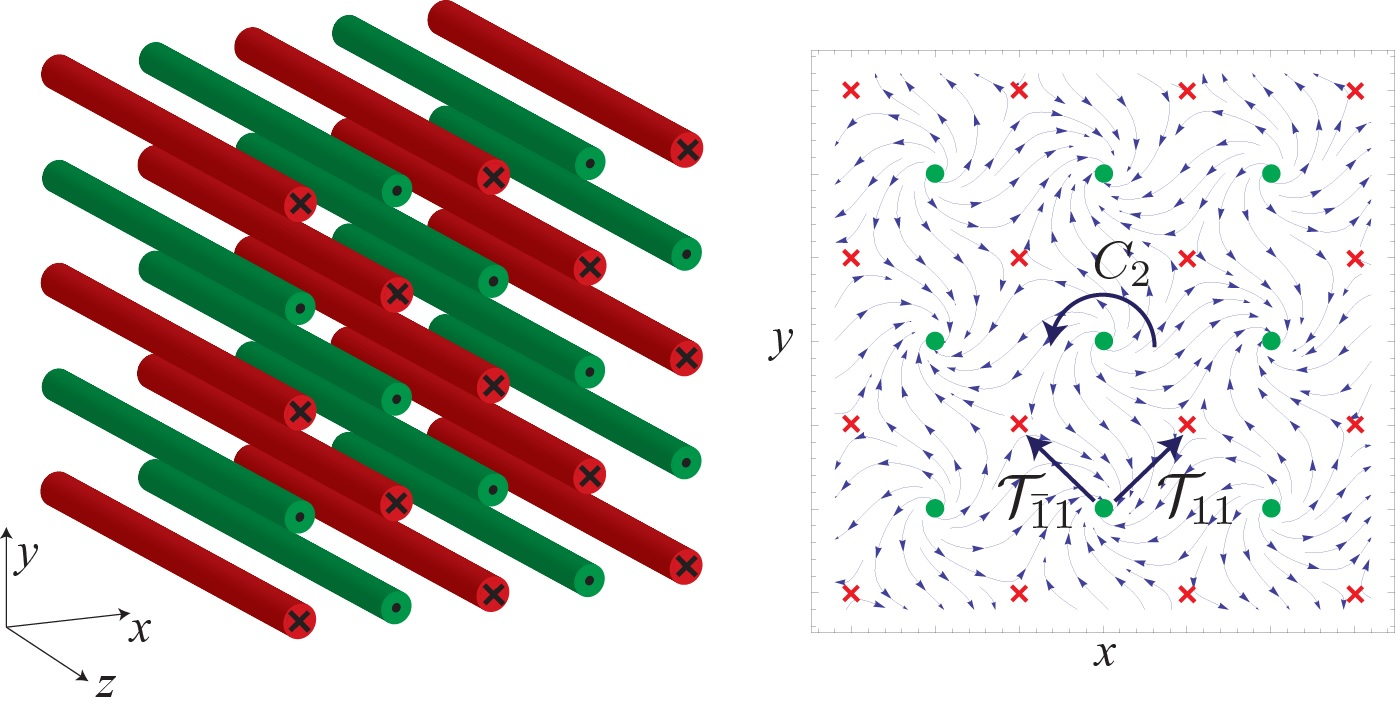
\includegraphics[width=0.45\textwidth]{vortexlattice.jpg}
\caption{(Left) A 3D array of Dirac strings. (Right) Cross section of the array. {\color{red}$\boldsymbol\times$} associates into-the-plane Dirac channel, {\color{green}$\bullet$} represents out-of-plane ones. Stream lines represent the configuration of the mass parameter vector field ${\bf m}({\bf r})=(m_x({\bf r}),m_y({\bf r}))$ of the vortex lattice.}\label{fig:vortexlattice}
\centering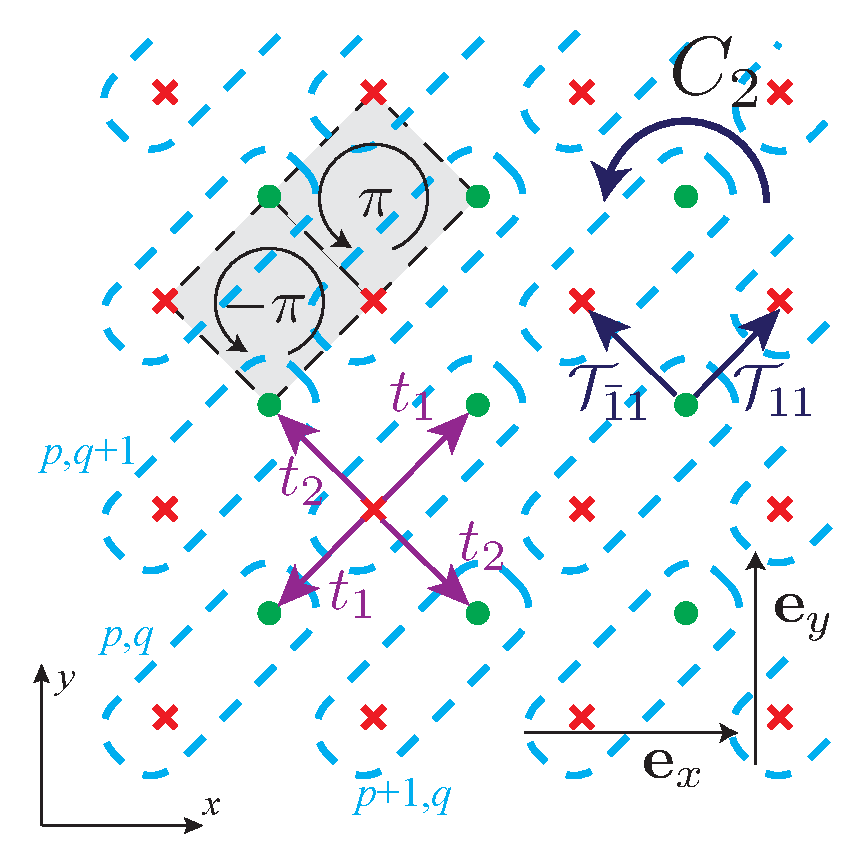
\includegraphics[width=0.25\textwidth]{WeylTB}
\caption{Coupled Dirac wire model with tunneling amplitudes $t_1,t_2$. Each unit cell (dashed box) consists a pair of counter-propagating Dirac strings, {\color{red}$\boldsymbol\times$} and {\color{green}$\bullet$}. $\mathcal{T}_{11},\mathcal{T}_{\bar{1}1}$ are the two anti-ferromagnetic directions.}\label{fig:WeylTB}
\end{figure}

A three-dimensional array of Dirac strings (wires) can be realized as a vortex lattice of the mass parameter $m=m_x+im_y$ in a Dirac semimetal. For example, figure~\ref{fig:vortexlattice} shows a vortex lattice generated by the spatially-varying Dirac mass \begin{align}m({\bf r})=m_0\frac{\mathrm{sd}(x+iy)}{|\mathrm{sd}(x+iy)|},\label{Jacobielliptic}\end{align} where $\mathrm{sd}$ is the (rescaled) Jacobian elliptic function~\cite{ReinhardtWalker10} with simple zeros at $p+iq$ and poles at $(p+1/2)+i(q+1/2)$ for $p,q$ integers. It consists of vortices with alternating winding number $c=\pm1$ at the zeros and poles in a checkered board lattice configuration. On the cross section plot on the right side of figure~\ref{fig:vortexlattice}, there is a Dirac string with positive (or negative) winding at each {\color{green}$\bullet$} (resp. {\color{red}$\boldsymbol\times$}). Each vortex string has a chiral Dirac fermion running through it. Figure~\ref{fig:WeylTB} shows the same two-dimensional slice of the array, except suppressing the mass parameters which correspond to irrelevant microscopic high-energy degrees of freedom. We choose a unit cell labeled by $(p,q)$, its $x,y$ coordinates. Each has both a forward moving Dirac fermion $\psi_{p,q}^\odot$ (shown as {\color{green}$\bullet$}) and a backward moving one $\psi_{p,q}^\otimes$ (shown as {\color{red}$\boldsymbol\times$}). 

This array configuration breaks time reversal as the symmetry would have reversed the chirality (i.e.~propagating direction) of each Dirac fermion. Instead, it has an emergent {\em anti-ferromagnetic time reversal} (AFTR) symmetry, which is generated by the operators $\mathcal{T}_{11}$ and $\mathcal{T}_{\bar{1}1}$ in the diagonal and off-diagonal directions. Each is composed of a time reversal operation and a half-translation by $({\bf e}_x+{\bf e}_y)/2$ or $(-{\bf e}_x+{\bf e}_y)/2$. \begin{gather}\mathcal{T}_{11}\psi_{p,q}^\otimes\mathcal{T}_{11}^{-1}=\psi_{p,q}^\odot,\quad\mathcal{T}_{11}\psi_{p,q}^\odot\mathcal{T}_{11}^{-1}=-\psi_{p+1,q+1}^\otimes\nonumber\\\mathcal{T}_{\bar{1}1}\psi_{p,q}^\otimes\mathcal{T}_{\bar{1}1}^{-1}=\psi_{p-1,q}^\odot,\quad\mathcal{T}_{\bar{1}1}\psi_{p,q}^\odot\mathcal{T}_{\bar{1}1}^{-1}=-\psi_{p,q+1}^\otimes\label{AFTR}\end{gather} These \AFTR operators are non-local as they come with lattice translation parts. They are anti-unitary in the sense that $\mathcal{T}\alpha\psi\mathcal{T}^{-1}=\alpha^\ast\mathcal{T}\psi\mathcal{T}^{-1}$ and $\langle\mathcal{T}u|\mathcal{T}v\rangle=\langle u|v\rangle^\ast$ because the local time reversal symmetry is anti-unitary. %Normally the local \TR operation for a spinful fermion squares to minus one. However, the non-local nature of the \AFTR symmetry allows us to absorb the sign by a non-local gauge transformation (for example $\psi^{\otimes/\odot}_{p,q}\to(-1)^q\psi^{\otimes/\odot}_{p,q}$) so that no signs appear in \eqref{AFTR}. 
Similar to a spatial non-symmorphic symmetry, the \AFTR symmetries square to the primitive translation operators \begin{align}\mathcal{T}_{11}\mathcal{T}_{\bar{1}1}&=(-1)^F\mbox{translation}({\bf e}_y),\nonumber\\\mathcal{T}_{11}\mathcal{T}_{\bar{1}1}^{-1}&=\mbox{translation}({\bf e}_x),\label{AFTRalg}\end{align} where $(-1)^F$ is the fermion parity operator. Moreover they mutually commute $[\mathcal{T}_{11},\mathcal{T}_{\bar{1}1}]=0$. We notice in passing that the \AFTR symmetry is only an emergent symmetry in the low-energy effective theory. It is not preserved in the microscopic Dirac model \eqref{DiracHam} and is broken by the mass parameter, $m({\bf r})\neq m({\bf r}+({\bf e}_x\pm{\bf e}_y)/2)^\ast$. For instance, the Jacobian elliptic Dirac mass function \eqref{Jacobielliptic} actually has a periodic unit cell twice the size of that of the effective wire model in figure~\ref{fig:WeylTB}. On the other hand, the Dirac mass \eqref{Jacobielliptic} is odd under $C_2$, $m(C_2{\bf r})=-m({\bf r})$. This sign is canceled by the $C_2$ rotations of the Dirac matrices, $\hat{C}_2\mu_{x,y}\hat{C}_2^{-1}=-\mu_{x,y}$, that couple with the Dirac mass in the Hamiltonian \eqref{DiracHam}. Therefore the Dirac wire model in figure~\ref{fig:WeylTB} has a twofold axis along one of the Dirac string, say $\psi^\odot_{0,0}$. The Dirac channel fermions transform unitarily according to \begin{align}\mathcal{C}_2\psi^\odot_{p,q}\mathcal{C}_2^{-1}=i\psi^\odot_{-p,-q},\quad\mathcal{C}_2\psi^\otimes_{p,q}\mathcal{C}_2^{-1}=-i\psi^\otimes_{-p+1,-q+1},\label{C2}\end{align} where the factor of $i$ ensures the fermionic $-1$ twist phase for a $2\pi$ rotation, and the second eqaulity in \eqref{C2} is determined by the first one together with \eqref{AFTR} and the symmetry relations \begin{gather}\mathcal{C}_2\mathcal{T}_{11}=(-1)^F\mathcal{T}_{11}^{-1}\mathcal{C}_2,\quad\mathcal{C}_2\mathcal{T}_{\bar{1}1}=(-1)^F\mathcal{T}_{\bar{1}1}^{-1}\mathcal{C}_2.\label{C2Trelation}\end{gather} Again, in order for the rotation symmetric wire model to be free of anomalies, $C_2$ should really be a screw rotation with respect to some microscopic lattice that has become irrelevant in the low-energy continuum picture. \begin{align}\mathcal{C}_2^2=(-1)^F\mathrm{translation}(a{\bf e}_z)\approx(-1)^F.\label{C2square}\end{align}

When adjacent vortex strings are near each other, their Dirac fermion wave functions overlap and there are finite amplitudes of electron tunneling. We construct a coupled Dirac wire model of nearest-wire single-body backscattering processes with $\pm\pi$ fluxes across each diamond square (figure~\ref{fig:WeylTB}), where the tunneling amplitude $t_1$ (or $t_2$) in the $(11)$ (resp.$(\bar{1}1)$) direction is imaginary (resp.~real). \begin{align}\mathcal{H}=&\sum_{p,q}\hbar\tilde{v}\left({\psi_{p,q}^\odot}^\dagger k_z\psi_{p,q}^\odot-{\psi_{p,q}^\otimes}^\dagger k_z\psi_{p,q}^\otimes\right)\nonumber\\&+it_1\left({\psi_{p,q}^\odot}^\dagger\psi_{p,q}^\otimes-{\psi_{p-1,q-1}^\odot}^\dagger\psi_{p,q}^\otimes\right)+h.c.\label{WeylTBHam}\\&+t_2\left({\psi_{p-1,q}^\odot}^\dagger\psi_{p,q}^\otimes-{\psi_{p,q-1}^\odot}^\dagger\psi_{p,q}^\otimes\right)+h.c.\nonumber\end{align} where the first line is the kinetic Hamiltonian of individual Dirac channels under the Fourier transformation $-i\partial_z\leftrightarrow k_z$ along the wire direction. This tight-binding Hamiltonian preserves the \AFTR symmetry \eqref{AFTR}, $\mathcal{T}\mathcal{H}\mathcal{T}^{-1}=\mathcal{H}$. Fourier transformation of the square lattice $\vec\psi_{p,q}=\int\frac{dk_xdk_y}{(2\pi)^2}e^{-i(k_xp+k_yq)}\vec\psi_{\bf k}$, $\vec\psi=(\psi^\odot,\psi^\otimes)$ turns \eqref{WeylTBHam} into $\mathcal{H}=\int\frac{dk_xdk_y}{(2\pi)^2}\vec\psi_{\bf k}^\dagger H(k)\vec\psi_{\bf k}$, where \begin{align}H({\bf k})=\left(\begin{array}{*{20}c}\hbar\tilde{v}k_z&g(k_x,k_y)\\g^\ast(k_x,k_y)&-\hbar\tilde{v}k_z\end{array}\right)\label{BlochHam}\end{align} is the Bloch band Hamiltonian, for $g(k_x,k_y)=it_1(1-e^{-i(k_y+k_x)})+t_2(e^{-ik_x}-e^{-ik_y})$. Here momentum ${\bf k}$ lives in the ``liquid crystal" Brillouin zone (\hypertarget{BZ}{BZ}) where $-\pi\leq k_x,k_y\leq\pi$ and $-\infty<k_z<\infty$ (in the continuum limit $a\to0$ and $\pi/a\to\infty$). 

\begin{figure}[htbp]
\centering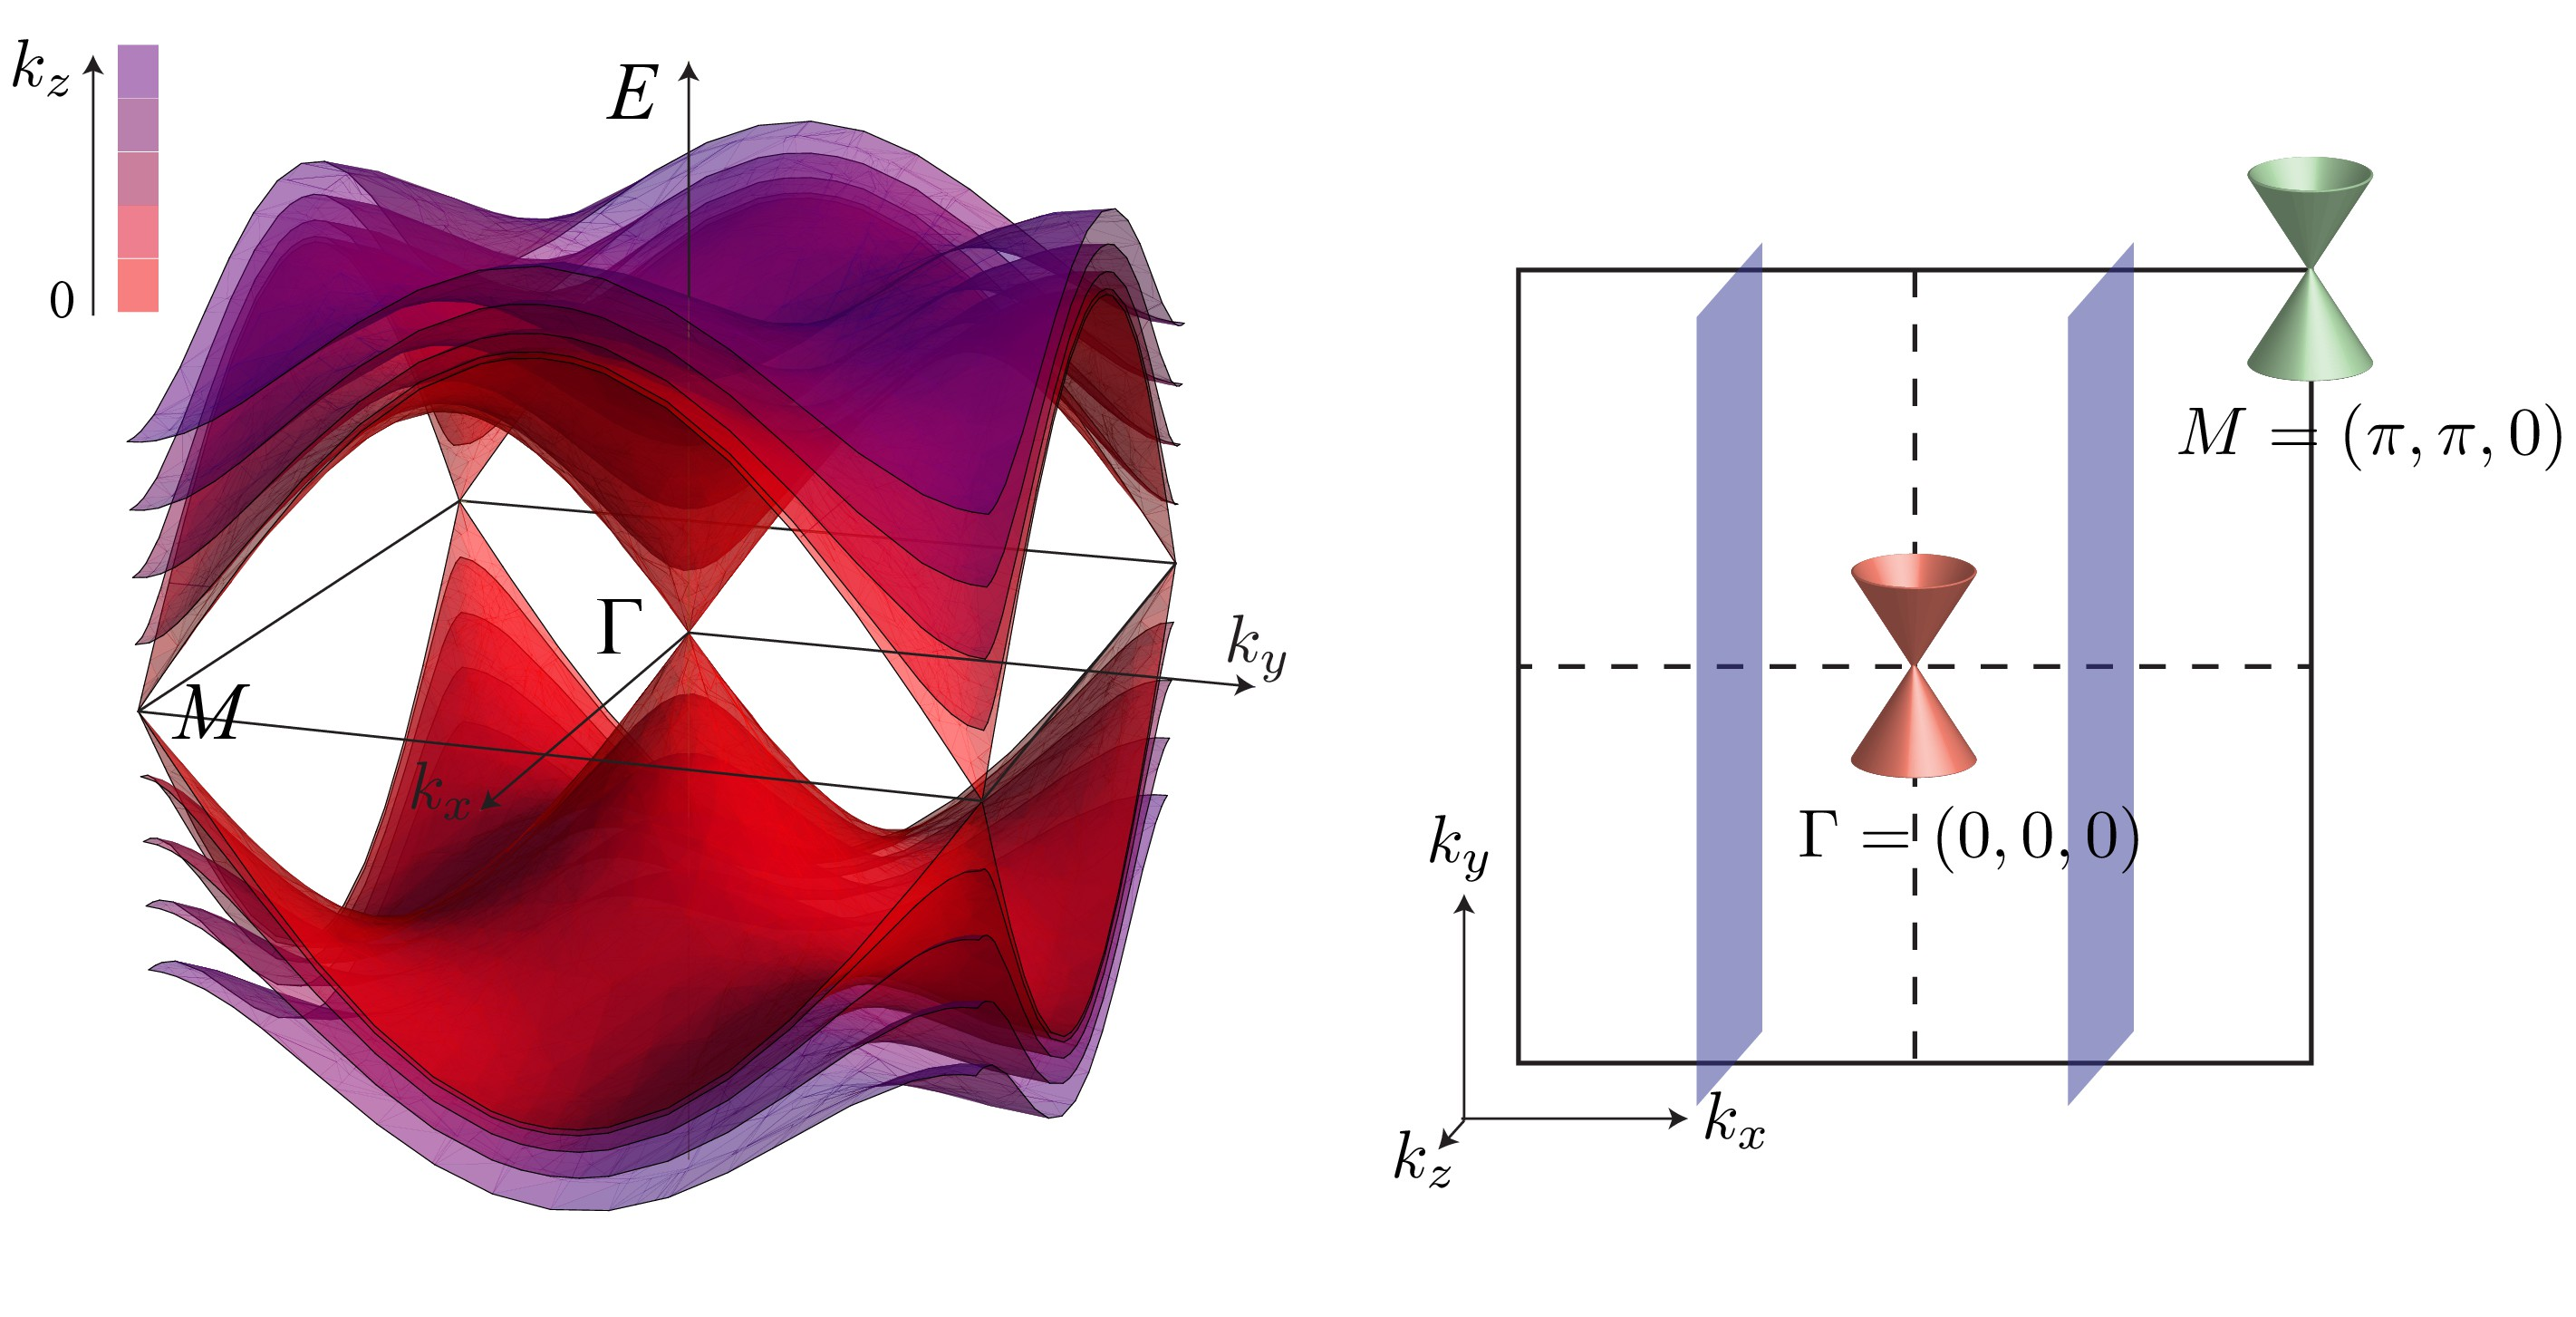
\includegraphics[width=0.45\textwidth]{Weylspectrumjpg.jpg}
\caption{Energy spectrum of the coupled Dirac wire model \eqref{WeylTBHam}.}\label{fig:Weylspectrum}
\end{figure}

The energy spectrum of the two-band model is given by $E_\pm({\bf k})=\pm\sqrt{|g(k_x,k_y)|^2+\hbar^2\tilde{v}^2k_z^2}$ (see figure~\ref{fig:Weylspectrum}).
It gives two linearly dispersing Weyl cones of opposite chiralities in the Brillouin zone centered at $K^+_0=\Gamma=(0,0,0)$ and $K^-_0=M=(\pi,\pi,0)$. Near these points, the Hamiltonians are of the linear form $H(K_0^\pm+\delta{\bf k})=\hbar\delta{\bf k}^TV^\pm\vec\sigma+O(\delta k^2)$, where $\vec\sigma=(\sigma_x,\sigma_y,\sigma_z)$ are Pauli matrices acting on the $(\psi^\odot,\psi^\otimes)$ degrees of freedom. The velocity matrices are \begin{align}\hbar V^\pm=\left(\begin{array}{ccc}-t_1&\pm t_2&0\\-t_1&\mp t_2&0\\0&0&\hbar\tilde{v}\end{array}\right),\end{align} whose determinant's %$\det(\hbar V)=\pm2\hbar\tilde{v}t_1t_2$ 
sign decides the $\pm$ chirality of the Weyl fermion at $\Gamma$ and $M$, i.e.~the $\pm1$ Fermi surface Chern invariants~\cite{WanVishwanathSavrasovPRB11,Ashvin_Weyl_review,RMP}. %Expanding about the two Weyl points and ignoring higher order terms gives $H(X^{\pm} + \delta {\mathbf{k}})= -t_1 (\delta k_x + \delta k_y) \sigma_x  \mp t_2 (\delta k_x - \delta k_y) \sigma_y  + v \delta k_z \sigma_z$.
The \AFTR symmetries \eqref{AFTR} in the single-body picture are expressed under Fourier transformation as \begin{gather}\mathcal{T}_{11}\vec\psi_{\bf k}\mathcal{T}_{11}^{-1}=T_{11}({\bf k})\vec\psi_{-\bf k},\quad\mathcal{T}_{\bar{1}1}\vec\psi_{\bf k}\mathcal{T}_{\bar{1}1}^{-1}=T_{\bar{1}1}({\bf k})\vec\psi_{-\bf k},\nonumber\\T_{11}({\bf k})=\left(\begin{array}{ccc}0&-e^{i(k_x+k_y)}\\1&0\end{array}\right)\mathcal{K},\nonumber\\T_{\bar{1}1}({\bf k})=\left(\begin{array}{ccc}0&-e^{ik_y}\\e^{-ik_x}&0\end{array}\right)\mathcal{K},\label{AFTRk}\end{gather} where $\mathcal{K}$ is the complex conjugation operator. They satisfy the appropriate algebraic relations \eqref{AFTRalg} in momentum space \begin{gather}T_{11}(-{\bf k})T_{\bar{1}1}({\bf k})=T_{\bar{1}1}(-{\bf k})T_{11}({\bf k})=-e^{-ik_y}\nonumber\\T_{11}(-{\bf k})T_{\bar{1}1}({\bf k})^{-1}=T_{\bar{1}1}(-{\bf k})^{-1}T_{11}({\bf k})=e^{-ik_x}\end{gather} and the coupled wire model \eqref{BlochHam} is \AFTR symmetric \begin{align}T_{11}({\bf k})H({\bf k})&=H(-{\bf k})T_{11}({\bf k}),\nonumber\\T_{\bar{1}1}({\bf k})H({\bf k})&=H(-{\bf k})T_{\bar{1}1}({\bf k}).\label{WeylTBT11}\end{align} The Weyl points are at time reversal invariant momenta (\hypertarget{TRIM}{TRIM}) $K^\pm_0\equiv-K^\pm_0$ (modulo the reciprocal lattice $2\pi\mathbb{Z}^2$), and the \AFTR operators $T_{11}(K^\pm_0)=-i\sigma_y\mathcal{K}$ and $T_{\bar{1}1}(K^\pm_0)=\mp i\sigma_y\mathcal{K}$ square to minus one. Hence the Weyl points are not only protected by the non-vanishing Fermi surface Chern invariant but also the Kramers' theorem. In addition, the model is also $C_2$ symmetric \begin{align}C_2({\bf k})H({\bf k})=H(C_2{\bf k})C_2({\bf k})\label{WeylTBC2}\end{align} where the twofold symmetry \eqref{C2} is represented in the single-body picture by a diagonal matrix \begin{align}\mathcal{C}_2\vec\psi_{\bf k}\mathcal{C}_2^{-1}=C_2({\bf k})\vec\psi_{\bf k},\quad C_2({\bf k})=\left(\begin{array}{*{20}c}i&0\\0&-ie^{-i(k_x+k_y)}\end{array}\right)\label{C2k}\end{align} (supressing the screw phase $e^{-ik_za/2}$ in the continuum limit $a\to0$). It agrees with the fermion statistics \eqref{C2square} $C_2(-k_x,-k_y,k_z)C_2(k_x,k_y,k_z)=-1$, and the algebraic relations \eqref{C2Trelation} with the \AFTR operators \begin{align}C_2(-{\bf k})T_{11}({\bf k})&=-T_{11}(C_2{\bf k})^{-1}C_2({\bf k})\nonumber\\C_2(-{\bf k})T_{\bar{1}1}({\bf k})&=-T_{\bar{1}1}(C_2{\bf k})^{-1}C_2({\bf k})\end{align} for $C_2{\bf k}=(-k_x,-k_y,k_z)$.

\subsubsection{The anomalous Dirac semimetal}\label{sec:anomaly}
We notice that the coupled wire Dirac model \eqref{WeylTBHam} and its massless energy spectrum in figure~\ref{fig:Weylspectrum} are anomalous with respect to the \AFTR symmetries $\mathcal{T}_{11}$ and $\mathcal{T}_{\bar{1}1}$ as well as the $C_2$ symmetry if it is proper symmorphic and not a screw rotation. This means that it cannot be realized in a single-body three dimensional lattice system with the \AFTR or $C_2$ symmetries. In a sense, it is not surprising at all since the chiral Dirac strings that constitute \eqref{WeylTBHam} are themselves violating fermion doubling~\cite{Nielsen_Ninomiya_1981,NielsenNinomiyaPLB1981}. Here we further elaborate on the anomalous Dirac spectrum (figure~\ref{fig:Weylspectrum}) where the pair of Weyl points are separately located at two time reversal invariant momenta $K^\pm_0$. We also comment on the non-trivial consequence of the anomaly and pave the path for later discussion on many-body interactions.

We begin with two 2D planes in momentum space parallel to $k_yk_z$ located at $k_x=\pm\pi/2$. They are represented by the two blue planes in figure~\ref{fig:Weylspectrum}. The \AFTR or $C_2$ symmetries require the Chern invariants \begin{align}\mathrm{Ch}_1=\frac{i}{2\pi}\int\mathrm{Tr}(P\partial_{k_y}P\partial_{k_z}P)dk_ydk_z\label{1stChern}\end{align} at $k_x=\pm\pi/2$ to be opposite, where $P({\bf k})=(\openone-H({\bf k})/|E({\bf k})|)/2$ is the projection operator onto the negative energy band. This is because the \AFTR symmetry is anti-unitary and preserves the orientation of the $k_yk_z$ plane, whereas $C_2$ is unitary but reverses the orientation of the $k_yk_z$ plane. Here we present a proof. 

We begin with a Bloch Hamiltonian $H({\bf k})$ that is symmetric under the operation $G({\bf k})$, \begin{align}H({\bf k})&=G(g{\bf k})H(g{\bf k})G(g{\bf k})^{-1}\end{align} if $G$ is unitary, or \begin{align}H({\bf k})&=G(g{\bf k})H(g{\bf k})^\ast G(g{\bf k})^{-1}\end{align} if it is antiunitary. Let $|u_m({\bf k})\rangle$ be the occupied states of $H({\bf k})$. We define $|u'_m({\bf k})\rangle=|Gu_m({\bf k})\rangle=G(g{\bf k})|u_m(g{\bf k})\rangle$ (or $|u'_m({\bf k})\rangle=|Gu_m({\bf k})\rangle=G(g{\bf k})|u_m(g{\bf k})^\ast\rangle$), which is also an occupied state of $H({\bf k})$, for unitary (resp.~antiunitary) symmetry.

The Chern number \eqref{1stChern} can equivalently be defined as \begin{align}\mathrm{Ch}_1(k_x)=\frac{i}{2\pi}\int_{\mathcal{N}_{k_x}}\mathrm{Tr}\left(\mathcal{F}_{\bf k}\right)\label{1stChernapp}\end{align} where $\mathrm{Tr}\left(\mathcal{F}_{\bf k}\right)=d\mathrm{Tr}\left(\mathcal{A}_k\right)$, $\mathcal{N}_{k_x}$ is the oriented $k_yk_z$-plane with fixed $k_x$, and $\mathcal{A}_k$ is the Berry connection of the occupied states $\mathcal{A}_{\bf k}^{mn}=\langle u_m({\bf k})|du_n({\bf k})\rangle$. The Berry connection transforms according to \begin{align}{\mathcal{A}'}_{\bf k}^{mn}&\equiv\langle u'_m({\bf k})|du'_n({\bf k})\rangle\\&=\langle u_m(g{\bf k})|G(g{\bf k})^\dagger d \left[G(g{\bf k})|u_n(g{\bf k})\rangle\right]\nonumber\\&=\mathcal{A}_{g{\bf k}}^{mn}+\langle u_m(g{\bf k})|\left[G(g {\bf k})^\dagger dG(g {\bf k})\right]|u_n(g{\bf k})\rangle\nonumber\end{align} for unitary $G$, or \begin{align}{\mathcal{A}'}_{\bf k}^{mn}&=\left(\mathcal{A}_{g{\bf k}}^{mn}\right)^\ast+\langle u_m(g{\bf k})^\ast|\left[G(g {\bf k})^\dagger dG(g {\bf k})\right]|u_n(g{\bf k})^\ast\rangle\nonumber\\&=-\mathcal{A}_{g{\bf k}}^{nm}+\langle u_m(g{\bf k})^\ast|\left[G(g {\bf k})^\dagger dG(g {\bf k})\right]|u_n(g{\bf k})^\ast\rangle\nonumber\end{align} if $G$ is antiunitary, because the connection is skew-hermitian $\mathcal{A}=-\mathcal{A}^\dagger$. Therefore \begin{align}%\mathrm{Tr}(\mathcal{A}'_{\bf k})&=\mathrm{Tr}(\mathcal{A}_{g{\bf k}})+\mathrm{Tr}\left\{P_{g \bf{k}}\wedge\left[G(g{\bf k})^\dagger dG(g {\bf k})\right]\right\},\nonumber\\
\mathcal{F}'_{\bf k}&=\mathcal{F}_{g{\bf k}}+d\mathrm{Tr}\left\{P_{g\bf{k}}\wedge\left(G(g{\bf k})^\dagger dG(g{\bf k})\right]\right\}\label{curvature}\end{align} for an unitary symmetry, or \begin{align}%\mathrm{Tr}(\mathcal{A}'_{\bf k})&=-\mathrm{Tr}(\mathcal{A}_{g{\bf k}})+\mathrm{Tr}\left\{P_{g \bf{k}}^\ast\wedge\left[G(g{\bf k})^\dagger dG(g {\bf k})\right]\right\},\nonumber\\
\mathcal{F}'_{\bf k}&=-\mathcal{F}_{g{\bf k}}+d\mathrm{Tr}\left\{P_{g\bf{k}}^\ast\wedge\left(G(g{\bf k})^\dagger dG(g{\bf k})\right]\right\}\label{curvature2}\end{align} for an antiunitary one. Here $P({\bf k})=\sum_n|u_n({\bf k})\rangle\langle u_n({\bf k})|$ is the projection operator on to the occupied energy states at momentum ${\bf k}$. Since the trace of Berry curvature $\mathrm{Tr}(\mathcal{F})$ does not depend on the gauge choice of occupied states, $\mathrm{Tr}(\mathcal{F}_{\bf k})=\mathrm{Tr}(\mathcal{F}'_{\bf k})$. We notice the final terms in both \eqref{curvature} and \eqref{curvature2} integrate to zero over the closed periodic momentum plane $\mathcal{N}_{k_x}$. This is because they are total derivatives, and unlike $\mathcal{A}_{\bf k}$, $P_{\bf k}$ and $G({\bf k})$ are defined non-singularly on the entire Brillouin zone (see \eqref{AFTRk} and \eqref{C2k}). 

Now we derive the relation between the Chern number \eqref{1stChernapp} between $k_x$ and $-k_x$ using the antiunitary \AFTR and the unitary $\mathcal{C}_2$ symmetries. The \AFTR symmetries flip all momentum axes $\mathcal{T}_{11},\mathcal{T}_{\bar{1}1}:(k_x,k_y,k_z)\mapsto(-k_x,-k_y,-k_z)$, while the $\mathcal{C}_2$ symmetry flips only two $\mathcal{C}_2:(k_x,k_y,k_z)\mapsto(-k_x,-k_y,k_z)$. Thus, $\mathcal{T}_{11},\mathcal{T}_{\bar{1}1}:\mathcal{N}_{k_x}\to\mathcal{N}_{-k_x}$ maps between opposite planes while preserving their orientations, but $\mathcal{C}_2:\mathcal{N}_{k_x}\to-\mathcal{N}_{-k_x}$ is orientation reversing. Lastly, we substitute \eqref{curvature} and \eqref{curvature2} into \eqref{1stChernapp}, and apply a change of integration variable ${\bf k}\leftrightarrow g{\bf k}$. The \AFTR and $\mathcal{C}_2$ requires the Chern number to flip under $k_x\leftrightarrow-k_x$ \begin{align}\mathrm{Ch}_1(k_x)=-\mathrm{Ch}_1(-k_x).\end{align}


 On the other hand, the two Chern invariants along the two planes must differ by 1 because they sandwich a single Weyl point at $\Gamma$. This forces the Chern invariants to be a half integer $\mathrm{Ch}_1=\pm1/2$, which is anomalous.

While the $C_2$ anomaly can be resolved simply by doubling the unit cell and assuming it originates from a microscopic non-symmorphic screw axis, the \AFTR anomaly is stronger because the two antiferromagnetic combinations \eqref{AFTRalg} generate lattice translations and fix the unit cell size. There are three resolutions. \begin{enumerate}\item The \AFTR symmetries are broken by high energy degrees of freedom when $k_z$ is large. \item The spectrum in figure~\ref{fig:Weylspectrum} is the holographic 3D boundary spectrum of an \AFTR symmetric weak topological insulator in 4D. \item The spectrum is generated by strong many-body interaction non-holographically in 3D.\end{enumerate} Below we discuss the first two resolutions, and we leave the many-body interaction-enabled situation to section~\ref{sec:intenable}.

\subsubsection{Broken symmetries and coarse-graining}\label{sec:brokensymmetry}
In the present case when the chiral Dirac channels originate from vortex strings in an underlying microscopic Dirac insulator, the spatial modulation of mass parameters $m({\bf r})$ actually violate one of the \AFTR symmetries, $m({\bf r})^\ast\neq m({\bf r}+({\bf e}_x\pm{\bf e}_y)/2)$, where $\ast$ stands for complex conjugation. For instance, since all elliptic functions must contain at least two zeros and two poles in its periodic cell, the Jacobian elliptic mass function \eqref{Jacobielliptic} has longer periods than ${\bf e}_x$ and ${\bf e}_y$ in figure~\ref{fig:WeylTB}, and thus must break $\mathcal{T}_{11}$ or $\mathcal{T}_{\bar{1}1}$. The symmetry is broken only in the ultra-violet limit at large $k_z$ where the chiral Dirac line nodes meet the microscopic bulk band (see figure~\ref{fig:Diracstring}) at high energy $\sim|m({\bf r})|$. In fact, the above anomalous argument shows that {\em all} mass parameter configurations that produce the 3D vortex lattice array (figure~\ref{fig:vortexlattice}) must either (a) break both the \AFTR symmetries $\mathcal{T}_{11}$ and $\mathcal{T}_{\bar{1}1}$, or (b) preserve one but violate translation so that the unit cell is enlarged and the two Weyl points collapse onto each other in momentum space. (See figure~\ref{fig:Chernstack} and \ref{fig:DiracTB}.)

For instance, the microscopic system can be connected to a stack of Chern insulating ribbons (or lowest Landau levels) with alternating chiralities shown in figure~\ref{fig:Chernstack}. Instead of being supported by vortices of Dirac mass, the chiral Dirac wires are now realized as edge modes of Chern insulating strips. Each 2D ribbon (represented by thick dashed dark blue lines) is elongated in the out-of-paper $z$-direction but is finite along the $(110)$ direction and holds counter-propagating boundary chiral Dirac channels. The dark blue arrows represent the orientations of the Chern ribbons that accommodate the boundary Dirac channels with the appropriate propagating directions. Here the Chern ribbon pattern in figure~\ref{fig:Chernstack}(a) breaks both \AFTR axes. The pattern in figure~\ref{fig:Chernstack}(b) preserves $\mathcal{T}_{\bar{1}1}$. However, translation symmetry is also broken and the coupled Dirac wire model now has an enlarged unit cell (light blue dashed boxes) that consists of two pairs of counter-propagating chiral Dirac channels. All Chern ribbon patterns must break the $C_2$ symmetry about a Dirac wire because each wire is connected to one and only one Chern ribbon in a particular direction.

\begin{figure}[htbp]
\centering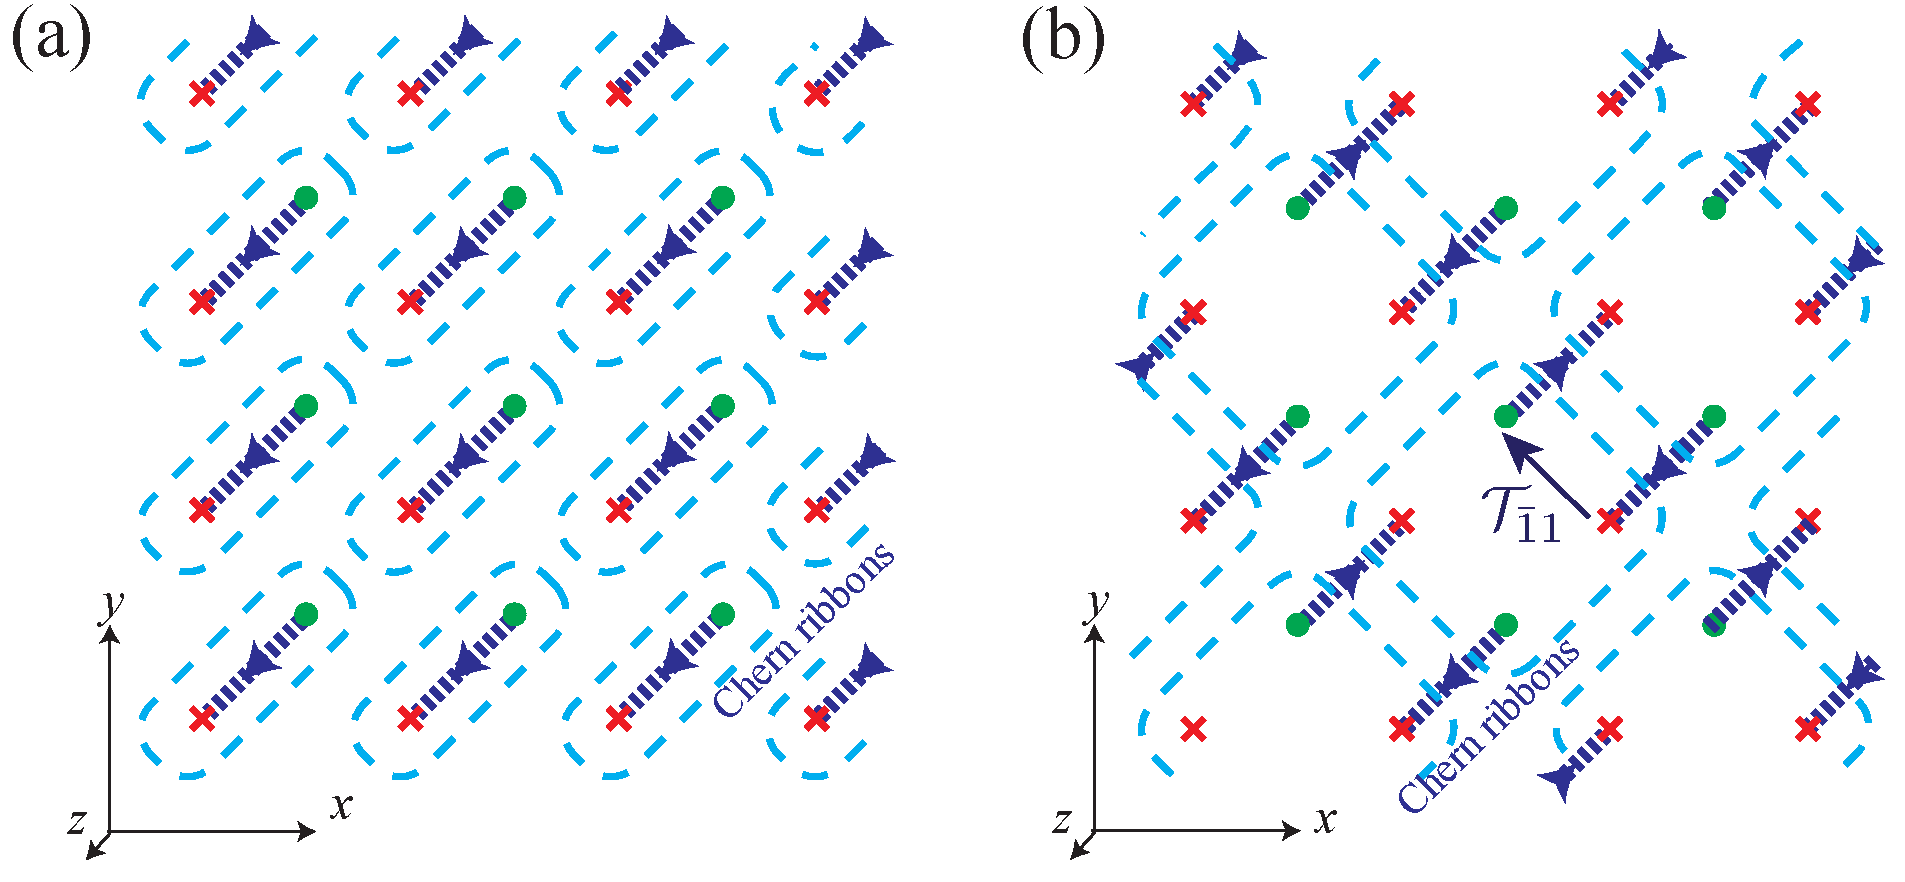
\includegraphics[width=0.45\textwidth]{Chernstack}
\caption{Chiral Dirac channels ({\color{red}$\boldsymbol\times$} and {\color{green}$\bullet$}) realized on the edge of Chern insulating ribbons (dark blue directed lines) stacked along the $(\bar{1}10)$ normal direction.}\label{fig:Chernstack}
\end{figure}

Now we go back to the vortex lattice generated by the Jacobian elliptic Dirac mass function $m({\bf r})$ in \eqref{Jacobielliptic} and consider its symmetries. For this purpose, we use the symmetry properties of the (rescaled) Jacobian elliptic function~\cite{ReinhardtWalker10} \begin{align}&\mathrm{sd}(x+iy)=-\mathrm{sd}(x+1+iy)=-\mathrm{sd}(x+iy+i)\nonumber\\&\mathrm{sd}\left(x+iy+\frac{1+i}{2}\right)=-i\frac{C}{\mathrm{sd}(x+iy)}\label{sdprop}\\&\mathrm{sd}(-x-iy)=-\mathrm{sd}(x+iy)\nonumber\end{align} where $C$ is some unimportant real constant that depends on the modulus of $\mathrm{sd}$ and will never appear in the mass function $m({\bf r})=m_0\mathrm{sd}(x+iy)/|\mathrm{sd}(x+iy)|$. We see from the minus sign in the first equation that the Jacobian elliptic function, and consequently the mass function, have primitive periods ${\bf e}_x\pm{\bf e}_y$ and therefore have a unit cell of size 2 (see figure~\ref{fig:DiracTB}(a)). Choosing $m_0=|m_0|e^{i\pi/4}$, we see from the second equation that $\mathcal{T}_{11}$ (or $\mathcal{T}_{\bar{1}1}$) is preserved (resp.~broken) \begin{align}m\left({\bf r}+\frac{{\bf e}_x\pm{\bf e}_y}{2}\right)=\pm m({\bf r})^\ast,\label{massT11}\end{align} and thus the parent Dirac Hamiltonian \eqref{DiracHam} is $\mathcal{T}_{11}$-symmetric \begin{align}\hat{T}H_{\mathrm{Dirac}}\left(-{\bf k},{\bf r}+\frac{{\bf e}_x+{\bf e}_y}{2}\right)\hat{T}^{-1}=H_{\mathrm{Dirac}}({\bf k},{\bf r}),\end{align} for $\hat{T}=is_y\mathcal{K}$. Lastly, the third property of \eqref{sdprop} entails the mass function $m({\bf r})=-m(C_2{\bf r})$ is odd under $C_2$, and consequently the parent Dirac Hamiltonian is (screw) rotation symmetric \begin{align}\hat{C}_2H_{\mathrm{Dirac}}(C_2{\bf k},C_2{\bf r})\hat{C}_2^{-1}=H_{\mathrm{Dirac}}({\bf k},{\bf r}),\label{massC2}\end{align} where $\hat{C}_2=is_z\mu_z$ (or microscopically $e^{-ik_za/2}is_z\mu_z$) anticommuting with the mass terms $m_1\mu_x+m_2\mu_y$ in $H_{\mathrm{Dirac}}$ (see \eqref{DiracHam}), and $C_2{\bf k}=(-k_x,-k_y,k_z)$, $C_2{\bf r}=(-x,-y,z)$.

\begin{figure}[htbp]
\centering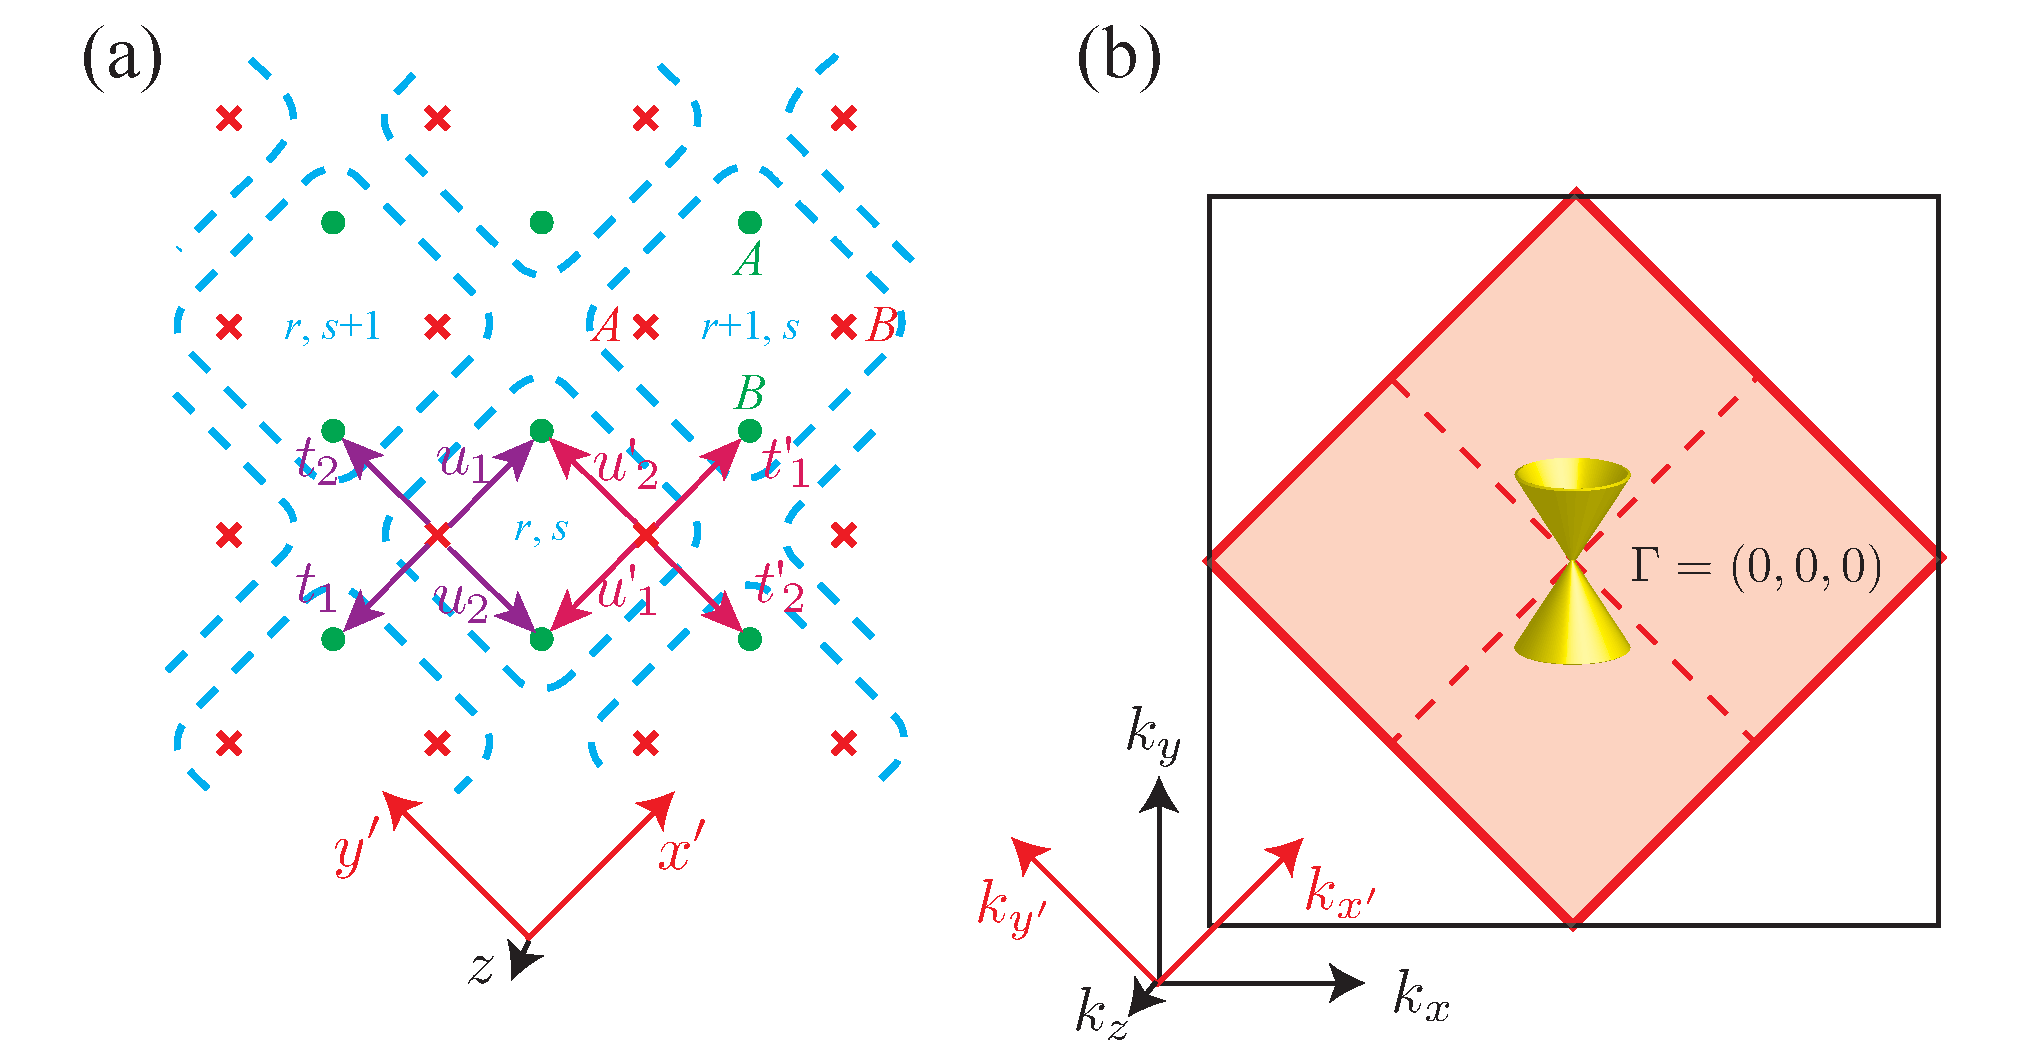
\includegraphics[width=0.45\textwidth]{DiracTB}
\caption{(a) The massive AFTR and $C_2$ breaking coupled Dirac wire model. (b) The reduced Brillouin zone (BZ) after translation symmetry breaking where the two Weyl points collapse to a single Dirac point at $M$.}\label{fig:DiracTB}
\centering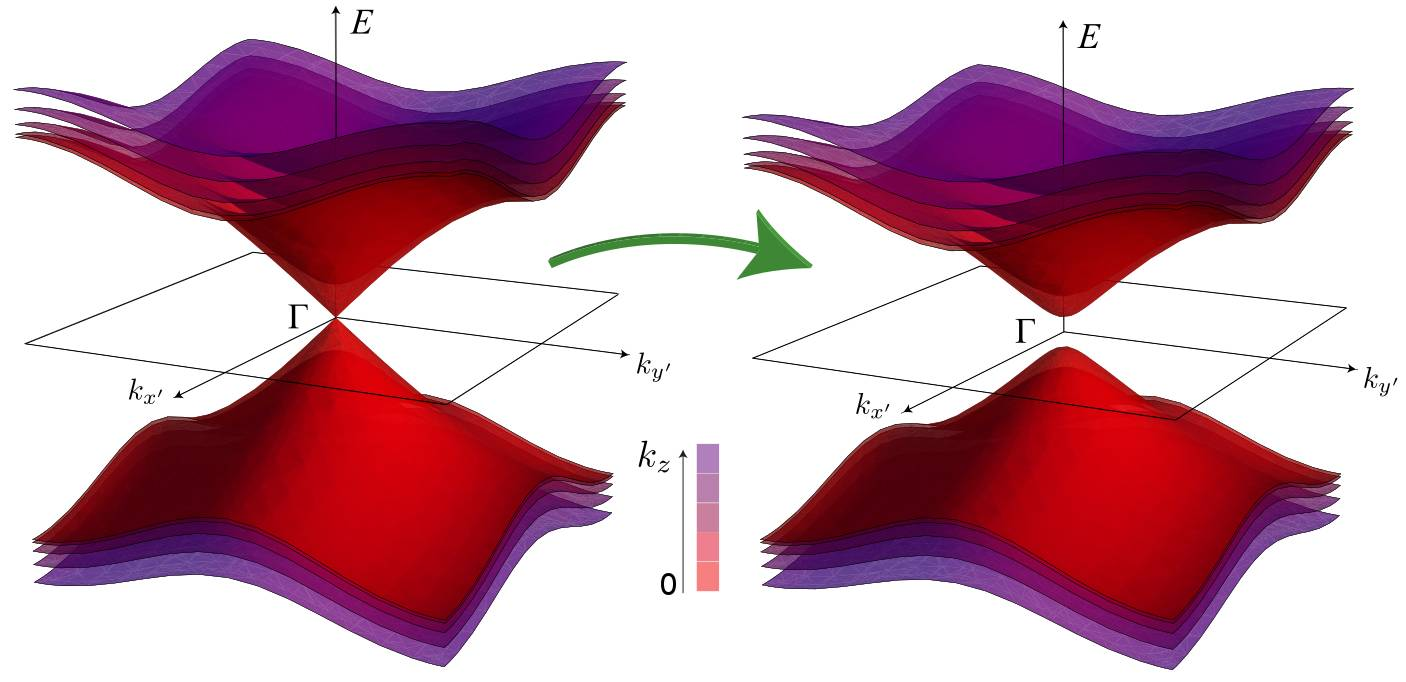
\includegraphics[width=0.48\textwidth]{Diracmassjpg.jpg}
\caption{Dirac mass gap $2|\Delta|$ introduced by AFTR and $C_2$ symmetry breaking dimerization $\Delta=\Delta_1+i\Delta_2$.}\label{fig:Diracmassjpg}
\end{figure}

Remembering that the coupled wire model \eqref{WeylTBHam} (figure~\ref{fig:WeylTB}) descended from a vortex lattice of the microscopic parent Dirac Hamiltonian \eqref{DiracHam}, the Dirac mass $m({\bf r})$ actually allows the model to carry fewer symmetries than the low-energy effective Hamiltonian \eqref{WeylTBHam} suggests. Now that the translation symmetry is lowered, the Brillouin zone is reduced (see figure~\ref{fig:DiracTB}(b)) so that the two Weyl points now coincide at the origin $\Gamma$. This recovers an unanomalous Dirac semimetallic model \eqref{DiracHam0} around $(k_{x'},k_{y'})=(0,0)$. The fourfold degenerate Dirac point is protected and pinned at $\Gamma$ due to the remaining \AFTR symmetry $\mathcal{T}_{11}$ -- which takes the role of a spinful time reversal ($\hat{T}^2=-1$) in the continuum limit -- and the $C_2$ (screw) symmetry about the $z$-axis. However, if any of these symmetries is further broken, the fourfold degeneracy of the Dirac point is not protected (c.f.~the original continuum Dirac model \eqref{DiracHam}). Figure~\ref{fig:DiracTB}(a) shows a dimerized coupled Dirac wire model that introduces a finite mass for the Dirac fermion. We label the Dirac fermion operators as $\psi_{r,s}^{\mu,\sigma}$, for $\sigma=\odot,\otimes$ the chirality, $\mu=A,B$ the new sublattice label, and $(r,s)$ label the coordinates of the unit cell according to the $45^\circ$-rotated $x',y'$-axes. \begin{align}\mathcal{H}'=&\sum_{r,s}\sum_{\mu=A,B}\hbar\tilde{v}\left({\psi_{r,s}^{\mu,\odot}}^\dagger k_z\psi_{r,s}^{\mu,\odot}-{\psi_{r,s}^{\mu,\otimes}}^\dagger k_z\psi_{r,s}^{\mu,\otimes}\right)\nonumber\\&+iu_1{\psi_{r,s}^{A,\odot}}^\dagger\psi_{r,s}^{A,\otimes}-iu'_1{\psi_{r,s}^{B,\odot}}^\dagger\psi_{r,s}^{B,\otimes}+h.c.\nonumber\\&-u_2{\psi_{r,s}^{B,\odot}}^\dagger\psi_{r,s}^{A,\otimes}+u'_2{\psi_{r,s}^{A,\odot}}^\dagger\psi_{r,s}^{B,\otimes}+h.c.\label{DiracTBHam}\\&-it_1{\psi_{r-1,s}^{A,\odot}}^\dagger\psi_{r,s}^{A,\otimes}+it'_1{\psi_{r+1,s}^{B,\odot}}^\dagger\psi_{r,s}^{B,\otimes}+h.c.\nonumber\\&+t_2{\psi_{r,s+1}^{B,\odot}}^\dagger\psi_{r,s}^{A,\otimes}-t'_2{\psi_{r,s-1}^{A,\odot}}^\dagger\psi_{r,s}^{B,\otimes}+h.c.\nonumber\end{align} For instance, the model is identical to the \AFTR and $C_2$ symmetric one in \eqref{WeylTBHam} when $t_j=t'_j=u_j=u'_j$ for $j=1,2$. However, when the symmetries are broken, these hopping parameters do not have to agree.

The Bloch band Hamiltonian after Fourier transformation is \begin{gather}H({\bf k})=\left(\begin{array}{*{20}c}\hbar\tilde{v}k_z\openone&h(k_{x'},k_{y'})\\h(k_{x'},k_{y'})^\dagger&-\hbar\tilde{v}k_z\openone\end{array}\right),\label{DiracBloch}\\h(k_{x'},k_{y'})=\left(\begin{array}{*{20}c}iu_1-it_1e^{-ik_{x'}}&u'_2-t'_2e^{-ik_{y'}}\\-u_2+t_2e^{ik_{y'}}&-iu'_1+it'_1e^{ik_{x'}}\end{array}\right)\nonumber\end{gather} where the $2\times2$ identity matrix $\openone$ and $h(k_{x'},k_{y'})$ acts on the sublattice $\mu=A,B$ degrees of freedom, and $-\pi\leq k_{x'},k_{y'}\leq\pi$ are the rotated momenta. We perturb about the Dirac fixed point by introducing the dimerizations $\Delta_j$ \begin{align}t_j=t'_j=u_j-\Delta_j=u'_j-\Delta_j\end{align} for $j=1,2$. About the $\Gamma=(0,0,0)$ point, \begin{align}H(\Gamma+\delta{\bf k})=&\hbar\tilde{v}\delta k_z\sigma_z-t_1\delta k_{x'}\sigma_x-t_2\delta k_{y'}\sigma_y\mu_x\nonumber\\&-\Delta_1\sigma_y\mu_z+\Delta_2\sigma_y\mu_y+O(\delta k^2).\label{DiracHamwire}\end{align} See figure~\ref{fig:Diracmassjpg} for its massive spectrum.

\begin{figure}[htbp]
\centering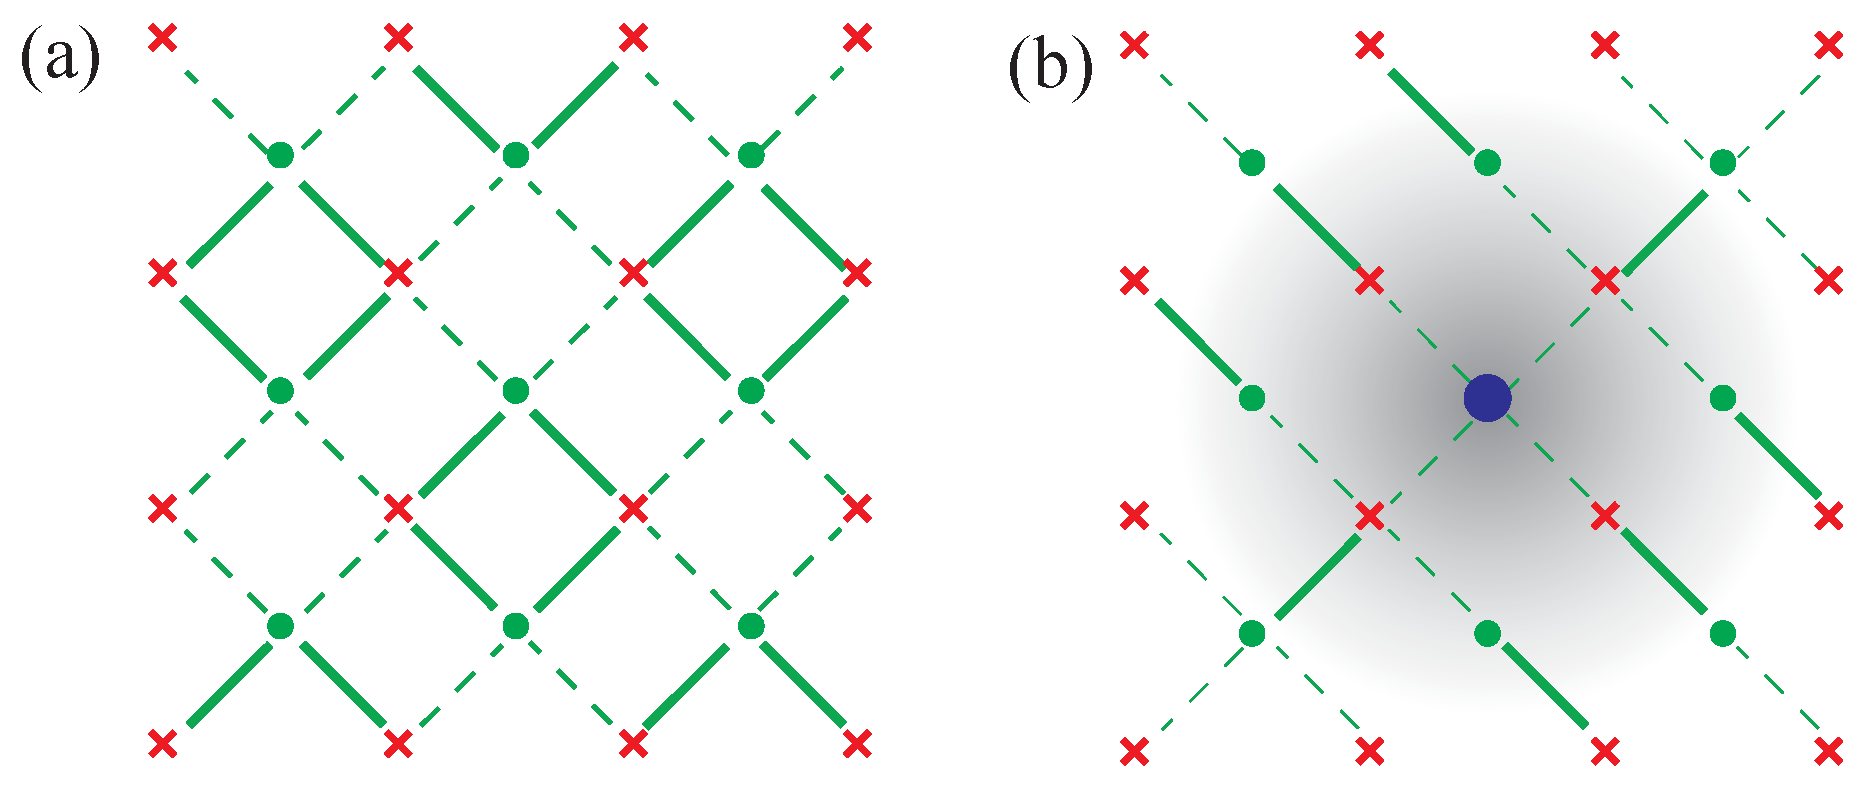
\includegraphics[width=0.4\textwidth]{dimerization}
\caption{(a) Dimerized model of a massive Dirac fermion. (b) Vortex of dimerizations $\Delta=\Delta_1+i\Delta_2$ that leaves behind a massless localized chiral Dirac channel (blue dot).}\label{fig:dimerization}
\end{figure}

Here the \AFTR symmetry $\mathcal{T}_{11}$ and the twofold rotation $\mathcal{C}_2$ are represented in the single-body picture by \begin{align}T_{11}({\bf k})&=\left(\begin{smallmatrix}0&0&-e^{ik_x}&0\\0&0&0&-1\\1&0&0&0\\0&e^{ik_x}&0&0\end{smallmatrix}\right)\mathcal{K},\nonumber\\C_2({\bf k})&=\left(\begin{smallmatrix}i&0&0&0\\0&ie^{-i(k_x+k_y)}&0&0\\0&0&-ie^{-ik_x}&0\\0&0&0&-ie^{-ik_y}\end{smallmatrix}\right)\end{align} (again suppressing the $C_2$ screw phase $e^{-ik_za/2}$ in the continuum limit $a\to0$). In the small $k_x,k_y$-limit, $T_{11}(0)=-i\sigma_y\mathcal{K}$ and $C_2(0)=i\sigma_z$. It is straightforward to check that the dimerization $\Delta_2$ preserves $\mathcal{T}_{11}$ while both $\Delta_1,\Delta_2$ breaks $C_2$.

Since the coupled wire model \eqref{DiracHamwire} and the parent continuum Dirac model \eqref{DiracHam} have the same matrix and symmetry structure, we can apply the same construction we discussed before to the new coarse-grained model \eqref{DiracHamwire}. For instance, the non-competing dimerizations $\Delta({\bf r})=\Delta_1({\bf r})+i\Delta_2({\bf r})$ can spatially modulate and form vortices in a longer length scale. Figure~\ref{fig:dimerization}(b) shows a dimerization pattern that corresponds to a single vortex in $\Delta$. The solid (dashed) lines represent strong (resp.~weak) backscattering amplitudes. In the fully dimerized limit where the dashed bonds vanish, all Dirac channels are gapped except the one at the center (showed as a blue dot). In the weakly dimerized case, there is a collective chiral Dirac channel whose wave function is a superposition of the original channels and is exponentially localized at the $\Delta$-vortex core, but now with a length scale longer than that of the original $m$-vortex lattice. These collective chiral Dirac $\Delta$-vortices can themselves form a coupled array, like \eqref{WeylTBHam}, and give a Dirac semimetal of even longer length scale. The single-body coupled vortex construction is therefore a coarse-graining procedure that recovers equivalent emergent symmetries at each step. \begin{align}\begin{diagram}\mbox{Dirac semimetal}&\pile{\rTo^{\mbox{\small mass vortices}}\\\lTo_{\mbox{\small coupled wire model}}}&\mbox{chiral Dirac strings}\end{diagram}\end{align}

\subsubsection{Holographic projection from 4D}\label{sec:holproj4D}
The coupled wire model \eqref{WeylTBHam} with two \AFTR axes can be supported by a weak topological insulator in four dimensions. Instead of realizing the chiral Dirac channels using mass vortices of a 3D Dirac semimetal, they can be generated as edge modes along the boundaries of 2D Chern insulators (or lowest Landau levels). The 4D weak topological insulator is constructed by stacking layers of Chern insulators parallel to the $zw$-plane along the $x$ and $y$ directions. The Chern layers $L_{\bf r}$, labeled by the checkerboard lattice vector ${\bf r}=r_x{\bf e}_x+r_y{\bf e}_y$ on the $xy$-plane, have alternating orientations so that $\mathrm{Ch}[L_{\bf r}]=1$ if $r_x,r_y$ are integers and $\mathrm{Ch}[L_{\bf r}]=-1$ if $r_x,r_y$ are half-integers.  The model therefore carries both \AFTR symmetries $\mathcal{T}_{11}$ and $\mathcal{T}_{\bar{1}1}$ as well as the $C_2$ rotation about $zw$, and when cleaved along a 3D hyper-surface normal to $w$, it generates the array of alternating chiral Dirac channels in figure~\ref{fig:WeylTB}.

The 4D weak topological insulator model can also be regarded as a stack of 3D antiferromagnetic topological insulators~\cite{MongEssinMoore10}. Restricting to the 3D hyperplane normal to $-{\bf e}_x+{\bf e}_y$, this model consists of alternating Chern insulating layers parallel to the $wz$-plane stacked along the ${\bf e}_x+{\bf e}_y$ direction. This 3D model describes an antiferromagnetic topologic insulator with a non-trivial $\mathbb{Z}_2$ index. For instance along the boundary surfaces normal to $w$ or $z$ that preserve the antiferromagnetic symmetry $\mathcal{T}_{11}$, the model leaves behind a 2D array of alternating chiral Dirac wires. The uniform nearest wire backscattering term $t_1$ (see \eqref{WeylTBHam}) introduces a linear dispersion along the $11$-direction and gives rise to a single massless surface Dirac cone spectrum at a time reversal invariant momenta on the boundary of the surface Brillouin zone where $\mathcal{T}_{11}^2=-1$. The 4D weak topological insulator model is identical to stacking these 3D antiferromagnetic topological insulators along the $\bar{1}1$-off-diagonal direction $-{\bf e}_x+{\bf e}_y$. A more detailed discussion on coupled wire constructions of a 4D strong and weak topological insulator can also be found in Ref.~\onlinecite{ParkTeoGilbertappearsoon}.

%A single wire with a chiral Dirac mode running through it is not allowed. Here we discuss what are the possible sources of chiral Dirac modes in our model. There are two possible sources, this three-dimensional array of chiral wires is the hypersurface of a four-dimensional Topological Insulator. The other possibility is that there are strips of Pfaffians, and each chiral Dirac mode (central charge c=1, conductance $\sigma$ = 1) is a combination of two adjacent edge modes of the Pfaffian strip (central charge c=1/2, conductance $\sigma$ = 1/2) as shown in fig.x. \textcolor{red}{insert a figure later}. Both of these cases preserve both of the TR operators $\mathcal{T}_{1 \bar{1}}$ and $\mathcal{T}_{1 {1}}$.

\subsubsection{AFTR breaking surfaces}\label{sec:fermiarcAFTRbreaking}

\begin{figure}[htbp]
\centering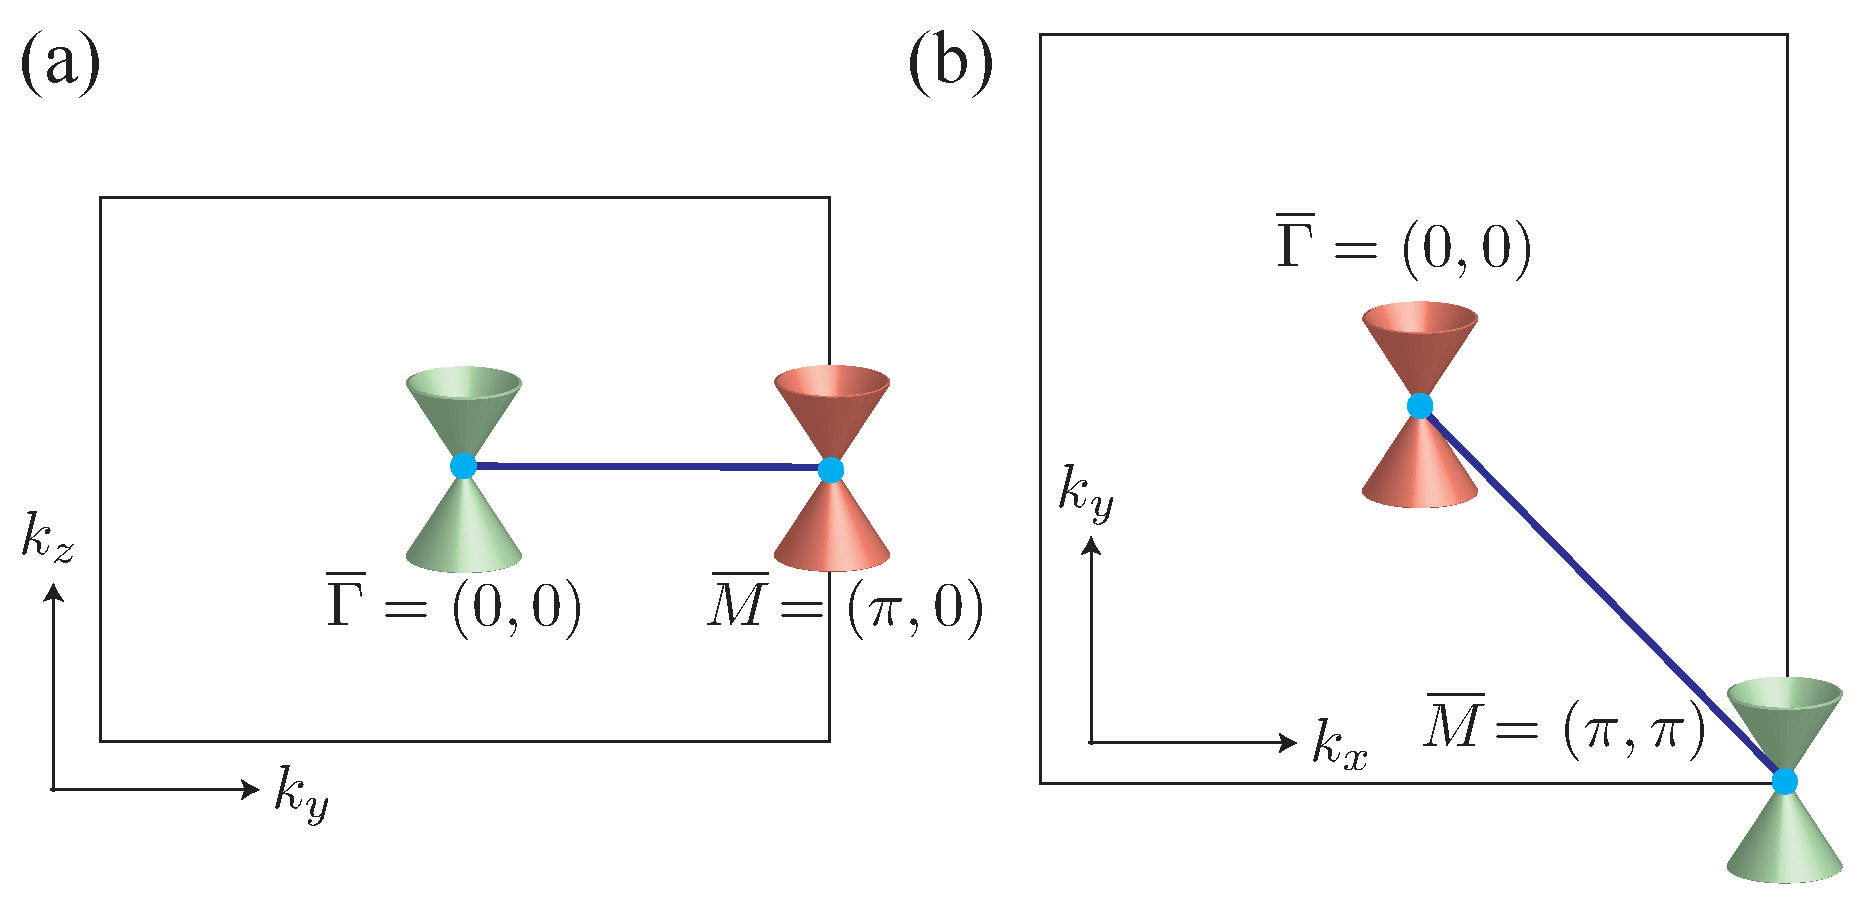
\includegraphics[width=0.4\textwidth]{fermiarc1}
\caption{Fermi arcs (blue lines) joining projected Weyl points on the surface Brillouin zones along (a) the $(100)$ surface and (b) the $(001)$ surface.}\label{fig:fermiarc1}
\end{figure}
We discuss the surface states of the coupled Dirac wire model \eqref{WeylTBHam}. Similar to the boundary surface of a translation symmetry protected Dirac semimetal (or more commonly called a Weyl semimetal), there are Fermi arcs connecting the surface-projected Weyl points~\cite{WanVishwanathSavrasovPRB11,Ashvin_Weyl_review,RMP}. First we consider the $(100)$ surface normal to $x$-axis (see figure~\ref{fig:WeylTB}). We assume the boundary cuts between unit cells and set the Fermi energy at $\varepsilon_f=0$. At $k_z=0$ and given a fixed $k_y\in(-\pi,\pi)$, the tight-binding model \eqref{BlochHam} is equivalent to the Su-Schriffer-Heeger model~\cite{SSH} or a 1D class AIII topological insulator~\cite{SchnyderRyuFurusakiLudwig08,Kitaevtable08} along the $x$-direction protected by the chiral symmetry $\sigma_zH(k_x)=-H(k_x)\sigma_z$. It is characterized by the winding number \begin{align}w(k_y)&=\frac{i}{2\pi}\int_{-\pi}^\pi \frac{1}{g(k_x,k_y)}\frac{\partial g(k_x,k_y)}{\partial k_x}dk_x\\&=\left(1+\mathrm{sgn}(k_y t_1/t_2)\right)/2.\nonumber\end{align} When $t_1,t_2$ have the same (or opposite) sign, the quasi-1D model is topological along the positive (resp.~negative) $k_y$-axis and thus carries a boundary zero mode. This corresponds to the Fermi line joining the two surface projected Weyl points at $\overline{\Gamma}$ and $\overline{M}$ (see figure~\ref{fig:fermiarc1}(a)). As the zero modes have a fixed chirality according to $\sigma_z$, they propagate uni-directionally with the dispersion $E(k_z)=\hbar\tilde{v}k_z\sigma_z$. The cleaving surface breaks \AFTR and $C_2$ symmetries, and so does the Fermi arc in figure~\ref{fig:fermiarc1}(a). For instance, any one of the \AFTR symmetries maps the boundary surface to an inequivalent one that cuts through unit cells instead of between them. As a result, the Fermi arc will connect the Weyl points along the opposite side of the $k_y$-axis for this surface. 

The $(010)$ surface Fermi arc structure is qualitatively equivalent to that of the $(100)$ surface. The $(110)$ and $(1\bar{1}0)$ surfaces that cleave along the diagonal and off-diagonal axes (see figure~\ref{fig:WeylTB}) respectively preserve the \AFTR symmetries $\mathcal{T}_{11}$ and $\mathcal{T}_{\bar{1}1}$. There are no protected surface Fermi arcs because the two bulk Weyl points project onto the same point on the surface Brillouin zone. Lastly, we consider the $(001)$ surface normal to the $z$-axis, which is the direction of the chiral Dirac strings that constitute the coupled wire model. A chiral Dirac channel cannot terminate on the boundary surface. In a single-body theory, it must bend and connect with an adjacent counter-propagating one. Although the $(001)$ plane is closed under the $C_2$ as well as both the \AFTR symmetries, the surface bending of Dirac channels must violate at least one of them. Here we consider the simplest case where the counter-propagating pair of Dirac channels within a unit cell re-connects on the boundary surface. This boundary is equivalent to a domain wall interface separating the Dirac semimetal \eqref{WeylTBHam} from an insulator where Dirac channels backscatters to their counter-propagating partner within the same unit cell. 

The domain wall Hamiltonian takes the form of a differential operator
\begin{align}\hat{\mathcal{H}}=&\sum_{m,j}-i\hbar\tilde{v}\left({\psi_{m,j}^\odot}^\dagger\partial_z\psi_{m,j}^\odot-{\psi_{m,j}^\otimes}^\dagger\partial_z\psi_{m,j}^\otimes\right)\label{WeylTBHamwall}\\&+it_1\left({\psi_{m,j}^\odot}^\dagger\psi_{m,j}^\otimes+\theta(z){\psi_{m-1,j-1}^\odot}^\dagger\psi_{m,j}^\otimes\right)+h.c.\nonumber\\&+t_2\theta(z)\left({\psi_{m-1,j}^\odot}^\dagger\psi_{m,j}^\otimes+{\psi_{m,j-1}^\odot}^\dagger\psi_{m,j}^\otimes\right)+h.c.\nonumber\end{align} by replacing $k_z\leftrightarrow-i\partial_z$ in \eqref{WeylTBHam}. Here $\theta(z)$ can be the unit step function or any function that asymptotically approaches 1 for $z\to\infty$ or 0 for $z\to-\infty$. The model therefore describes the Dirac semimetal \eqref{WeylTBHam} for positive $z$, and an insulator for negative $z$ where Dirac channels are pair annihilated within a unit-cell by $t_1$. After a Fourier transformation, the Bloch Hamiltonian $\hat{H}(k_x,k_y)$ is identical to \eqref{BlochHam} by replacing $k_z\leftrightarrow-i\partial_z$ and $g(k_x,k_y,z)=it_1(1+\theta(z)e^{-i(k_y+k_x)})+t_2\theta(z)(e^{-ik_x}+e^{-ik_y})$. Given any fixed $k_x,k_y$, the differential operator $\hat{H}(k_x,k_y)$ is identical to the Jackiw-Rebbi model~\cite{JackiwRebbi76}. Deep in the insulator, $g(k_x,k_y,z\to-\infty)=it_1$. There is an interface zero mode at the surface domain wall if $g$ changes sign, i.e.~if $g(k_x,k_y,z\to\infty)=|g|e^{i\varphi}$ has argument $\varphi=-\mathrm{sign}(t_1)\pi/2$. When $\varepsilon_f=0$, the zero modes trace out a Fermi arc that connects the two surface projected Weyl points (see figure~\ref{fig:fermiarc1}(b)).

\begin{figure}[htbp]\centering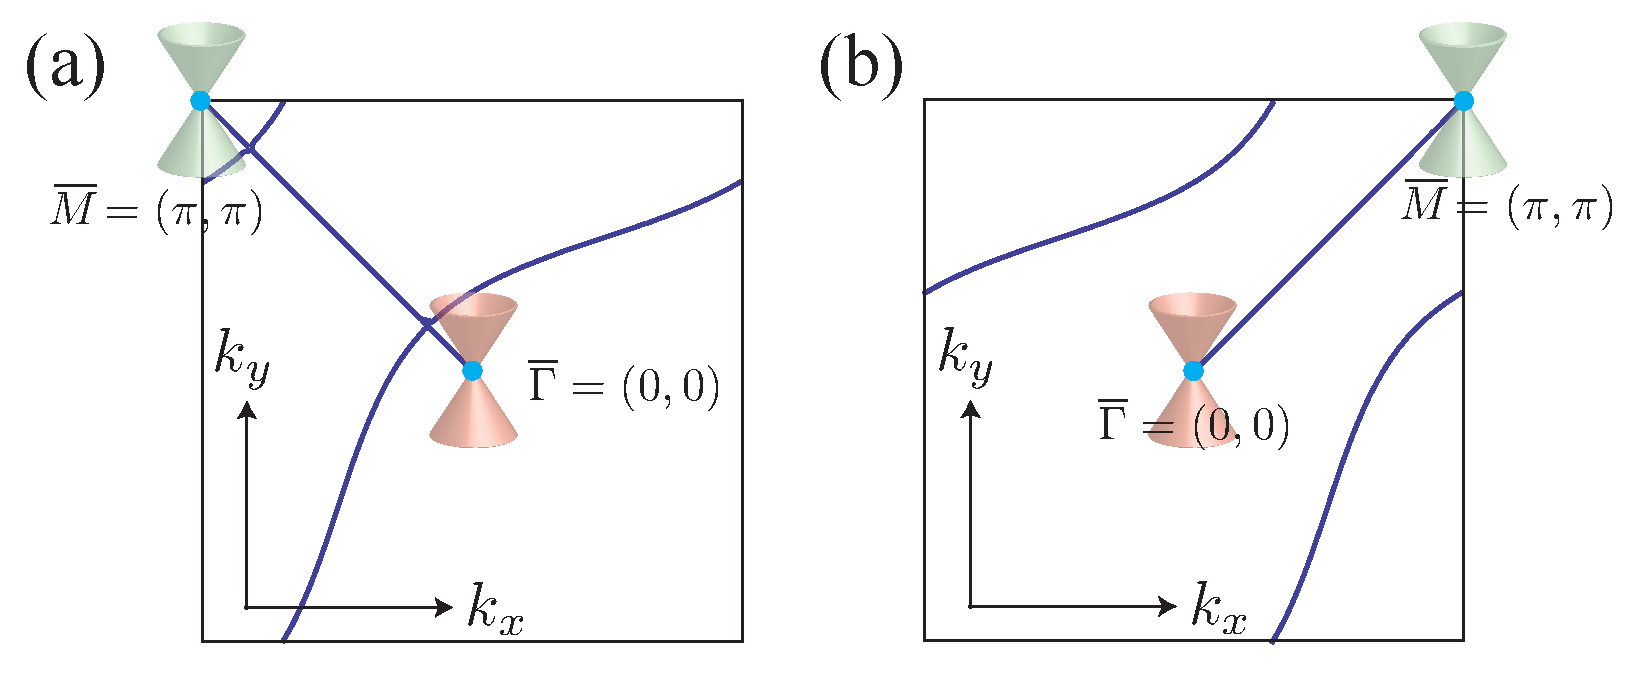
\includegraphics[width=0.4\textwidth]{fermiarc2}\caption{Fermi arcs (blue lines) on the $(001)$ surface with alternative boundary conditions (a) $g(k_x,k_y)=-it_1$ and (b) $g(k_x,k_y)=-t_2e^{-ik_y}$ in the insulating domain, for $t_2/t_1=2$.}\label{fig:fermiarc2}\end{figure}

We notice that in the insulating phase (or on the boundary surface), Dirac wires can be backscattered with a different phase and dimerized out of the unit cell. These different boundary conditions correspond to distinct surface Fermi arc patterns. Figure~\ref{fig:fermiarc2} shows two alternatives. (a) shows the the zero energy arcs when intra-cell backscattering reverses sign $t_1\to-t_1$ in the insulating domain. (b) shows a case when the dimerization is taken along the off-diagonal axis. These inequivalent boundary conditions differ by some three dimensional integer quantum Hall states, which correspond to additional chiral Fermi arcs that wrap non-trivial cycles around the 2D toric surface Brillouin zone.

\subsubsection{AFTR preserving surfaces}\label{sec:fermiarcAFTRpreserving}

We also notice that the Fermi arc structures in figures~\ref{fig:fermiarc1}(b) and \ref{fig:fermiarc2} are allowed because both the \AFTR symmetries $\mathcal{T}_{11}$, $\mathcal{T}_{\bar{1}1}$ and the $C_2$ symmetry are broken by the insulating domain. Any dimerization that preserves only one of $\mathcal{T}_{11}$ and $\mathcal{T}_{\bar{1}1}$ necessarily breaks translation symmetry, and corresponds to an enlarged unit cell and a reduced Brillouin zone (c.f.~figure~\ref{fig:Chernstack} and \ref{fig:DiracTB}). As a result, the two Weyl points would now collapse onto the same $\overline{\Gamma}$ point. Any momentum plane that contains the $k_z$-direction and avoids the $\Gamma$ point must have trivial Chern invariant, because it could always be deformed (while containing the $k_z$-direction and avoiding the $\Gamma$ point) to the reduced Brillouin zone boundary, where its Chern invariant would be killed by the \AFTR symmetry. %There would therefore be no protected surface Fermi arcs.

However, the trivial bulk Chern invariant does not imply the absence of surface state. This can be understood by looking at the surface boundary in real space. Here, we assume the Dirac strings that constitute the coupled wire model \eqref{WeylTBHam} are supported by vortices of an underlying Dirac mass (see figure~\ref{fig:vortexlattice} and eq.\eqref{DiracHam}). The semimetallic coupled wire model terminates along the $xy$-plane against vacuum, which is modeled by the Dirac insulator $H_{\mathrm{vacuum}}=\hbar v{\bf k}\cdot\vec{s}\mu_z+m_0\mu_x$, say with $m_0>0$. Recall from \eqref{massT11} that the Dirac mass vortex configuration \eqref{Jacobielliptic} is \AFTR symmetric along the $\mathcal{T}_{11}$-directions. The Dirac insulating vacuum is symmetric under local time reversal as well as continuous translation. It however breaks the screw rotation symmetry $\hat{C}_2=is_z\mu_z$, but we here only focus on the \AFTR symmetry.

\begin{figure}[htbp]
\centering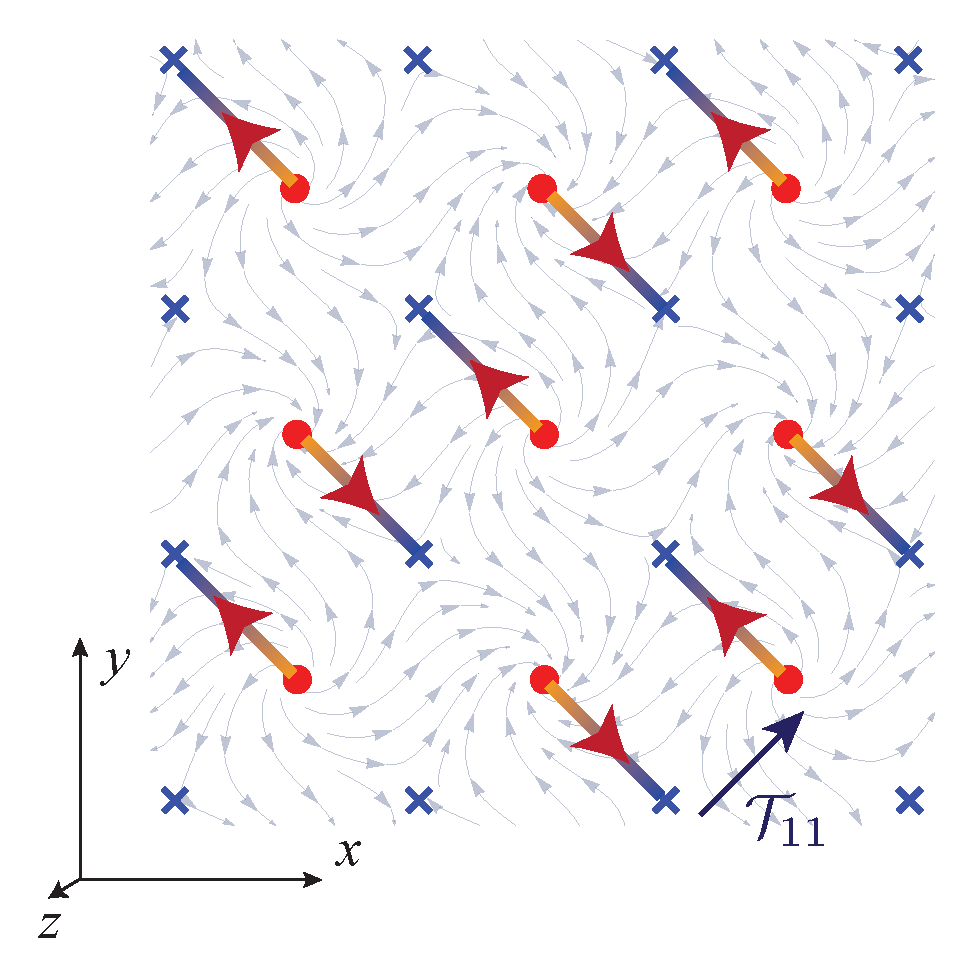
\includegraphics[width=0.3\textwidth]{SurfaceStates1bdy}
\caption{Surface chiral Dirac channels of the coupled wire model \eqref{WeylTBHam} terminated along the $xy$ plane.}\label{fig:SurfaceStates1bdy}
\end{figure}

The surface boundary supports chiral Dirac channels that connect the chiral Dirac strings in the semimetallic bulk that are normal to the surface. The surface channels are shown in figure~\ref{fig:SurfaceStates1bdy}. The {\color{blue}$\times$} ({\color{red}$\bullet$}) represent chiral vortices in the bulk that direct electrons away from (resp.~onto) the surface. The vector field represents the Dirac mass $m({\bf r})=m_x({\bf r})+im_y({\bf r})$ modulation in the semimetallic bulk near the surface. The surface Dirac line channels~\cite{TeoKane} -- shown by directed lines connecting the bulk Dirac strings {\color{blue}$\times$}, {\color{red}$\bullet$} -- are located where the time reversal symmetric Dirac mass $m_x$ changes sign across the surface boundary and the time reversal breaking Dirac mass $m_y$ flips sign across the line channels along the surface. In other words, they are traced out of points on the surface where $m_x<0$ and $m_y=0$. Each of these surface channels carries a chiral Dirac electronic mode that connects the bulk chiral Dirac vortices. They can couple through inter-channel electron tunneling, but the collective gapless surface state cannot be removed from low-energy by dimerization without breaking the \AFTR symmetry $\mathcal{T}_{11}$. %The surface state is, in a sense, half of that of a weak topological insulator (or 3D stack of quantum spin Hall layers). 

\subsection{Many-body interacting variations}\label{sec:interaction}
We discuss the effect of strong many-body interactions in a Dirac semimetal in three dimensions. Before we do so, it is worth stepping back and reviewing the two dimensional case in order to illustrate the issue and idea that will be considered and generalized in three dimensions. The massless Dirac fermion with $H=\hbar v(k_xs_y-k_ys_x)$ that appears on the surface of a topological insulator~\cite{HasanKane10,QiZhangreview11,HasanMoore11,RMP} is protected by time reversal (TR) and charge $U(1)$ symmetries and is anomalous. This means that there is no single-body energy gap opening mass term that preserves the symmetries, and there is no single-body fermionic lattice model in two dimensions that supports a massless Dirac fermion without breaking the symmetries. Neither of these statements hold true in the many-body setting. The surface Dirac fermion can acquire a time reversal and charge $U(1)$ preserving many-body interacting mass.~\cite{WangPotterSenthilgapTI13,ChenFidkowskiVishwanath14,MetlitskiKaneFisher13b,BondersonNayakQi13} Consequently, this also enables a massless symmetry preserving Dirac fermion in a pure 2D system without holographically relying on a semi-infinite 3D topological bulk. For instance, one can take a quasi-2D topological insulator slab with finite thickness and remove the Dirac fermion on one of the two surfaces by introducing an interacting mass gap. This leaves a single massless Dirac fermion on the opposite surface without breaking symmetries.

A massless Dirac fermion in three dimensional semimetallic materials can be protected in the single-body picture by screw rotation, time reversal and charge $U(1)$ symmetries (see reviews Ref.~\onlinecite{Ashvin_Weyl_review,RMP,ArmitageMeleVishwanath16} and section~\ref{sec:DiracSemimetal}). From a theory point of view, it can be supported on the 3D boundary of a 4D weak topological insulator, where the two Weyl fermions are located at distinct time reversal invariant momenta (recall figure~\ref{fig:Weylspectrum} and section~\ref{sec:holproj4D} for the antiferromagnetic case). In this case, the massless fermions are protected by translation, time reversal and charge $U(1)$ symmetries. In this section, we address the following issues. (1) We show by explicitly constructing an exactly solvable coupled wire model that the 3D Dirac fermion can acquire a many-body interacting mass while preserving all symmetries. (2) We show in principle that an antiferromagnetic time reversal (AFTR) symmetric massless 3D Dirac system with two Weyl fermions separated in momentum space can be enabled by many-body interactions without holographically relying on a higher dimensional topological bulk.

We begin with the Dirac semimetallic coupled wire model in figure~\ref{fig:Weylspectrum} and \eqref{WeylTBHam}.  


\subsubsection{Symmetry preserving massive interacting model}\label{sec:interactionmodels}

We begin with the 3D array of chiral Dirac strings in figure~\ref{fig:vortexlattice}. In section~\ref{sec:DiracSemimetal}, we showed that the single-body coupled wire model \eqref{WeylTBHam} described a Dirac semimetal with two Weyl fermions (see figure~\ref{fig:Weylspectrum}). The system had emergent antiferromagnetic time reversal (AFTR) symmetries $\mathcal{T}_{11}$ and $\mathcal{T}_{\bar{1}1}$ along the diagonal and off-diagonal axes (see \eqref{WeylTBT11}). Together they generate an emergent lattice translation symmetry with a 2-wire unit cell, and separate the two Weyl points in the Brillouin zone. The symmetries are lowered beyond the effective model when the microscopic high-energy degrees of freedom are included. For example, the mass function \eqref{Jacobielliptic} that supports the Dirac vortex string lattice has a 4-wire periodic unit cell and only preserves one of the \AFTR symmetries $\mathcal{T}_{11}$ (see \eqref{massT11}). With the lowered translation symmetry, the two Weyl points now coincide at the same momentum. Inter-species (or inter-valley) mixing is forbidden by the remaining \AFTR symmetry and a (screw) twofold rotation symmetry $C_2$ about $z$ (see \eqref{WeylTBC2} and \eqref{massC2}). Previously in section~\ref{sec:brokensymmetry}, we introduced symmetry breaking wire dimerizations in \eqref{DiracTBHam} that led to a massive Dirac insulator. In this section, we construct many-body gapping interactions that preserves the two \AFTR symmetries $\mathcal{T}_{11}$ and $\mathcal{T}_{\bar{1}1}$, the $C_2$ symmetry, as well as charge $U(1)$ conservation. 

\begin{figure}[htbp]
\centering
(a)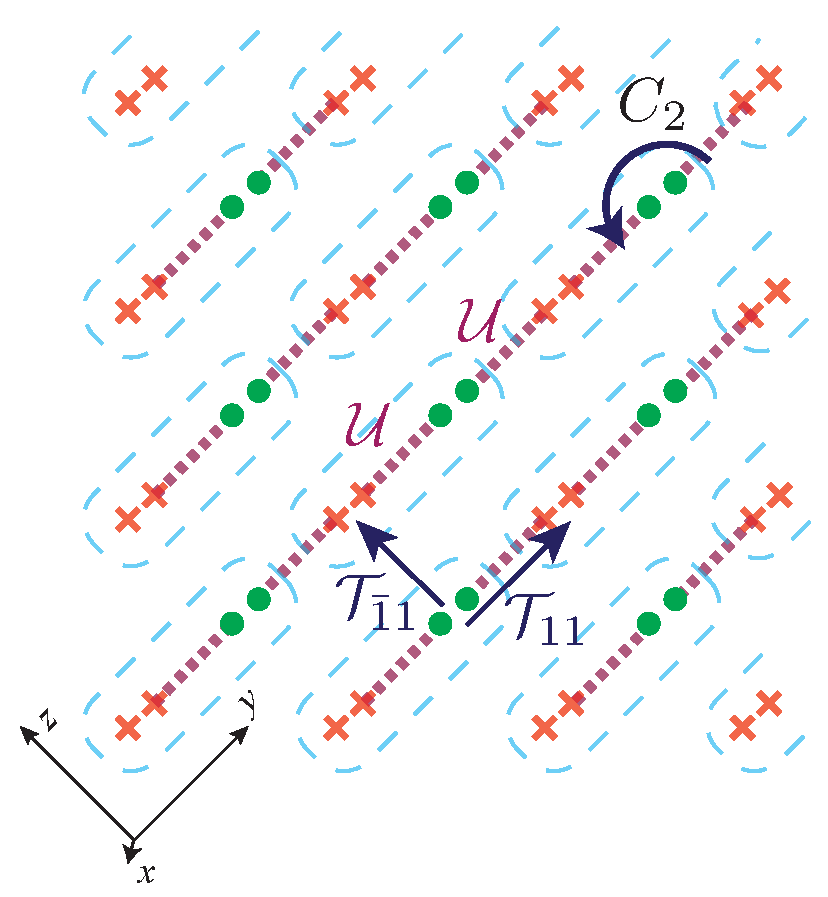
\includegraphics[width=0.25\textwidth]{gappinginteraction1}
(b)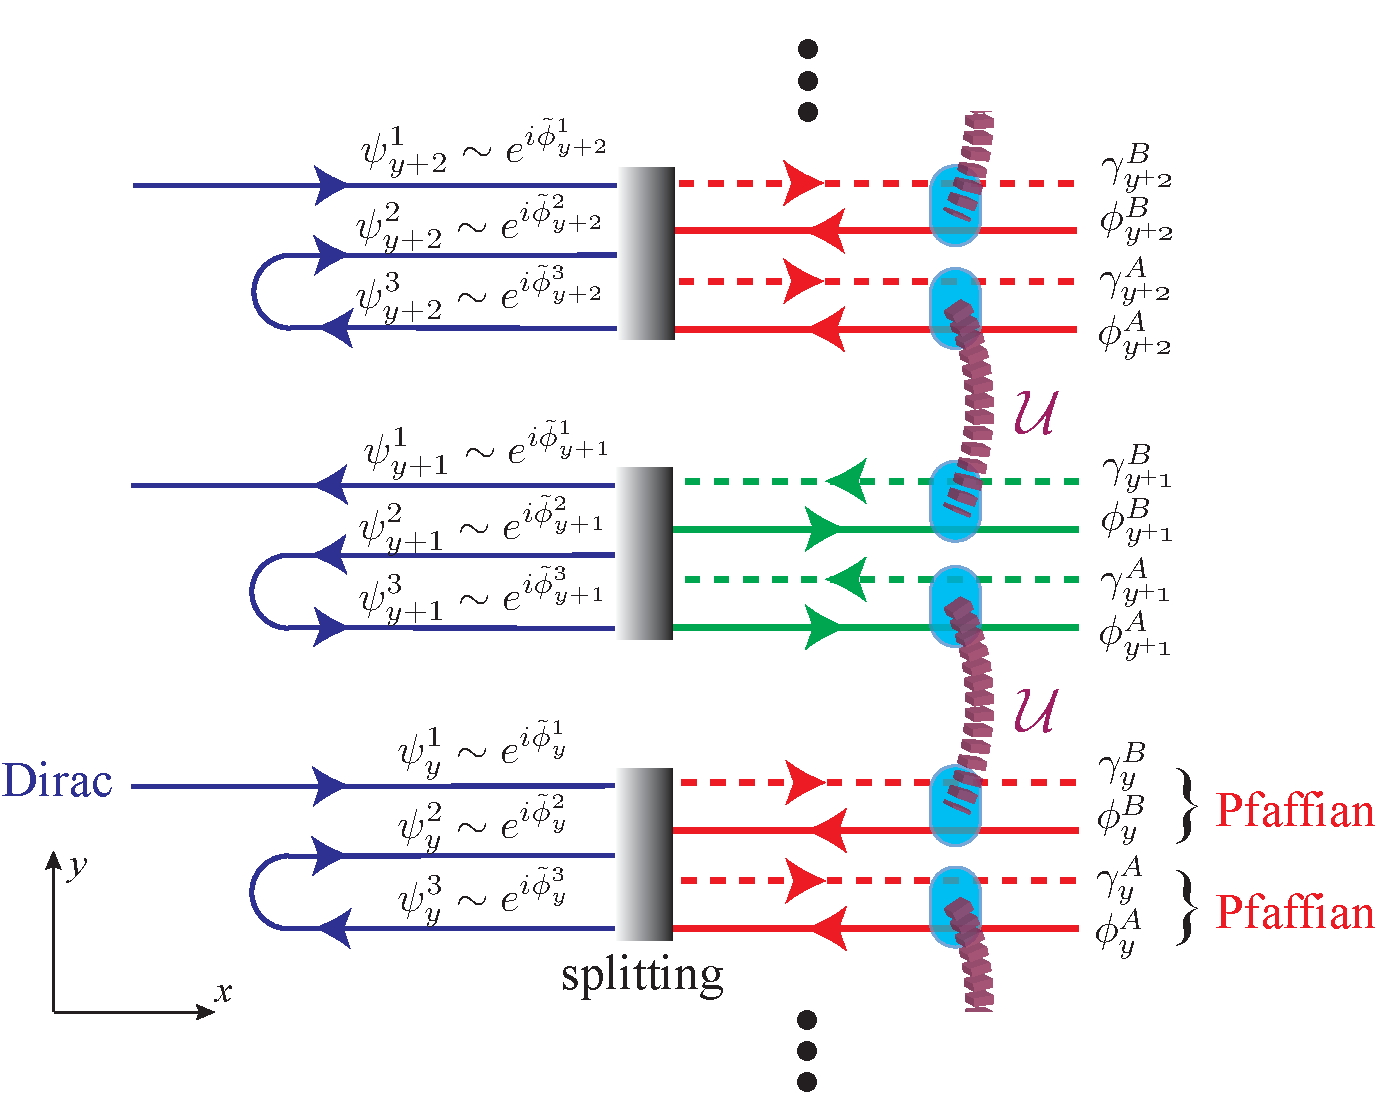
\includegraphics[width=0.45\textwidth]{gappinginteraction2}
\caption{Symmetry preserving many-body gapping interaction. (a) Each {\color{red}$\boldsymbol\times$}/{\color{green}$\bullet$} represents a chiral Pfaffian channel into/out-of paper. Purple dashed line represents many-body gapping interaction $\mathcal{U}$ in \eqref{mbdint}. (b) Coupled wire model on a single layer along the diagonal axis.}\label{fig:gappinginteraction}
\end{figure}

The many-body gapping scheme is summarized in figure~\ref{fig:gappinginteraction}. From the previous subsection, we saw that each chiral Dirac channel can be decomposed into a pair of independent Pfaffian channels. They can then be backscattered in opposite directions to neighboring wires. Figure~\ref{fig:gappinginteraction}(a) shows a particular dimerization pattern of the Pfaffian channels that preserves the symmetries. In this case, the many-body backscattering interaction $\mathcal{U}$ is directed along the diagonal axis. In the limit when $\mathcal{U}$ is much stronger than the single-body electron tunneling in the previous semimetallic model \eqref{WeylTBHam}, the system decomposes into decoupled diagonal layers and it suffices to consider the interaction on a single layer. For convenience, we here change our spatial coordinates so that the diagonal axis is now labeled by $y$ and the wires now propagate along $x$.

Focusing on a single diagonal layer, the system in the non-interacting limit first consists of a 2D array of chiral Dirac strings with alternating propagating directions (see the left side of figure~\ref{fig:gappinginteraction}(b)). We notice that this is identical to the starting point of the coupled wire construction of the topological insulator Dirac surface state considered by Mross, Essin and Alicea in Ref.~\onlinecite{MrossEssinAlicea15}. For instance, the alternating Dirac channels there were supported between magnetic strips with alternating orientations on the topological insulator surface, and an uniform nearest-channel electron tunneling recovered the massless 2D Dirac spectrum protected by the \AFTR symmetry. They then proceeded to propose symmetry preserving many-body gapping interactions facilitated by adding 2D fractional quantum hall strips between the channels. While this reconstruction trick can be applied on the 2D surface of a topological insulator, it is not feasible in our 3D situation and would require drastic modification of the bulk semimetal. Instead, here we propose an alternative gapping scheme that does not involve additional topological phases. In other words, we are going to construct a 3D gapped and layered topological phase solely from interacting electronic Dirac wires.

First, in order to implement the splitting described in the previous subsection, we assume each Dirac string consists of two Dirac channels going in one direction and a third Dirac channel going the opposite direction (see the left side of figure~\ref{fig:gappinginteraction}(b)). We denote the electronic Dirac fermions on the $y^{\mathrm{th}}$ wire by $\boldsymbol\psi_y=(\psi_y^1,\psi_y^2,\psi_y^3)$ and bosonize \begin{align}\psi_y^{1,2}(x)\sim e^{i\tilde\phi^{1,2}_y(x)},\quad\psi_y^3(x)\sim e^{-i\tilde\phi^3_y(x)}.\label{bosondef}\end{align} The sliding Luttinger liquid\cite{OHernLubenskyToner99,EmeryFradkinKivelsonLubensky00,VishwanathCarpentier01,SondhiYang01,MukhopadhyayKaneLubensky01} Lagrangian density is \begin{align}\mathcal{L}_{\mathrm{layer}}=\sum_{y=-\infty}^\infty\frac{(-1)^y\tilde{K}_{jk}}{2\pi}\partial_t\tilde\phi_y^j\partial_x\tilde\phi_y^k+\tilde{V}_{jk}\partial_x\tilde\phi_y^j\partial_x\tilde\phi_y^k\label{Llayer}\end{align} where $\tilde{K}=(\tilde{K}_{jk})_{3\times3}=\mathrm{diag}(1,1,-1)$, $\tilde{V}$ is some non-universal velocity matrix, and repeating species indices $j,k$ are summed over. The boson operators obey the equal-time commutation relation (\hypertarget{ETCR}{ETCR}) \begin{align}&\left[\tilde\phi_y^j(x),\tilde\phi_{y'}^{j'}(x')\right]=c^{jj'}_{yy'}(x-x')\nonumber\\=&i\pi(-1)^y\delta_{yy'}\tilde{K}^{jj'}\mathrm{sgn}(x'-x)\label{ETcomm0}\\&+i\pi(-1)^y\delta_{yy'}S^{jj'}\nonumber\\&+i\pi(-1)^{\mathrm{max}\{y,y'\}}\mathrm{sgn}(y-y')\Sigma^{jj'}\sigma_z^{y-y'+1}\nonumber\end{align}
%\begin{align}\left[\tilde\phi_y^j(x),\tilde\phi_{y'}^{j'}(x')\right]=&i\pi(-1)^{\mathrm{max}\{y,y'\}}\Big[\delta_{yy'}\tilde{K}^{jj'}\mathrm{sgn}(x'-x)\nonumber\\&+\delta_{yy'}\mathrm{sgn}(j-j')+\mathrm{sgn}(y-y')\Big]\label{ETcomm0}\end{align} 
where $\mathrm{sgn}(s)=s/|s|=\pm1$ for $s\neq0$ and $\mathrm{sgn}(0)=0$, \begin{align}S=\left(\begin{smallmatrix}0&1&-1\\-1&0&1\\1&-1&0\end{smallmatrix}\right),\quad\Sigma=\left(\begin{smallmatrix}1&1&-1\\1&1&-1\\-1&-1&1\end{smallmatrix}\right),\label{Kleinfactors}\end{align} and $\sigma_z=\pm1$. The introduction of the specific Klein factors $S^{jj'}$, $\Sigma^{jj'}$ and the undetermined sign $\sigma_z$ are necessary for the correct representations of the $\mathcal{T}_{11}$ and $\mathcal{C}_2$ symmetries in the bosonization setting, and these choices will be justified below. The first line of \eqref{ETcomm0} is equivalent to the commutation relation between conjugate fields \begin{align}\left[\tilde\phi_y^j(x),\partial_{x'}\tilde\phi_{y'}^{j'}(x')\right]=2\pi i(-1)^y\delta_{yy'}\tilde{K}^{jj'}\delta(x-x')\label{ETcomm00}\end{align} which is set by the ``$p\dot{q}$" term in $\mathcal{L}_{\mathrm{layer}}$. The alternating signs $(-1)^y$ in \eqref{ETcomm00} and \eqref{Llayer} changes the propagating directions from wire to wire. The second and third line of \eqref{ETcomm0} guarantee the correct anticommutation relations $\{e^{\pm i\tilde\phi^j_y},e^{\pm i\tilde\phi^{j'}_{y'}}\}=0$ between Dirac fermions along distinct channels $j\neq j'$ or distinct wires $y\neq y'$. The reason the $\tilde{C}_2$ matrix is defined in this form will become clear in the fractional basis discussed later in \eqref{bosonC2Pf}.

The anti-unitary \AFTR symmetry along the diagonal $\mathcal{T}_{11}$ direction transforms the bosons according to \begin{align}\mathcal{T}_{11}\tilde\phi^j_y\mathcal{T}_{11}^{-1}=-\tilde\phi^j_{y+1}+\frac{1+(-1)^y}{2}\tilde{K}^{jj}\pi.\label{bosonTR11}\end{align} The unitary $\mathcal{C}_2$ rotation takes \begin{gather}\mathcal{C}_2\tilde\phi^j_y\mathcal{C}_2^{-1}=\left(\tilde{C}_2\right)^j_{j'}\tilde\phi^{j'}_{-y}+(-1)^yv^j\frac{\pi}{2},\label{bosonC2}\\\tilde{C}_2=\left(\begin{smallmatrix}1&2&2\\2&1&2\\-2&-2&-3\end{smallmatrix}\right),\quad{\bf v}=\left(\begin{smallmatrix}v^1\\v^2\\v^3\end{smallmatrix}\right)=\left(\begin{smallmatrix}3\\-3\\1\end{smallmatrix}\right).\nonumber\end{gather} Moreover, we choose the representation so that the sign $\sigma_z$ in the equal time commutation relations \eqref{ETcomm0} is preserved by the \AFTR operator but is flipped by the $C_2$ symmetry, \begin{align}\mathcal{T}_{11}\sigma_z\mathcal{T}_{11}^{-1}=\sigma_z,\quad\mathcal{C}_2\sigma_z\mathcal{C}_2^{-1}=-\sigma_z.\end{align} 

The equal time commutation relations \eqref{ETcomm0} is consistent with the \AFTR symmetry. This means that evaluating $\mathcal{T}_{11}\left[\tilde\phi_y^j(x),\tilde\phi_{y'}^{j'}(x')\right]\mathcal{T}_{11}^{-1}$ by taking the \AFTR operator inside the commutator \begin{align}&\left[\mathcal{T}_{11}\tilde\phi_y^j(x)\mathcal{T}_{11}^{-1},\mathcal{T}_{11}\tilde\phi_{y'}^{j'}(x')\mathcal{T}_{11}^{-1}\right]\nonumber\\&=\left[\tilde\phi_{y+1}^j(x),\tilde\phi_{y'+1}^{j'}(x')\right]=c^{jj'}_{y+1,y'+1}(x-x')\end{align} yields the same outcome as taking the time reversal of the purely imaginary scalar \begin{align}\mathcal{T}_{11}c^{jj'}_{yy'}(x-x')\mathcal{T}_{11}^{-1}=-c^{jj'}_{yy'}(x-x').\end{align} The equal time commutation relations \eqref{ETcomm0} is also consistent with the $\mathcal{C}_2$ symmetry \begin{align}(\tilde{C}_2)^{j_1}_{j'_1}c^{j'_1j'_2}_{-y_1,-y_2}(x_1-x_2)(\tilde{C}_2)^{j_2}_{j'_2}=\mathcal{C}_2c^{j_1j_2}_{y_1y_2}(x_1-x_2)\mathcal{C}_2^{-1}.\label{ETcommC2consistent}\end{align} This is because the Klein factors \eqref{Kleinfactors} are $C_2$ symmetric \begin{align}\tilde{C}_2S\tilde{C}_2^T=S,\quad\tilde{C}_2\Sigma\tilde{C}_2^T=\Sigma.\end{align} Notice that the undetermined sign $\sigma_z$, which is odd under $\mathcal{C}_2$, in \eqref{ETcomm0} is essential for the equal time commutation relations to be consistent with $C_2$.

The last term in the \AFTR operation \eqref{bosonTR11} makes sure \begin{align}\mathcal{T}_{11}^2\tilde\phi_y^j(x)\mathcal{T}_{11}^{-2}=\tilde\phi_{y+2}^j+(-1)^y\tilde{K}^{jj}\pi,\end{align} which is necessary for $\mathcal{T}^2_{11}=(-1)^F\mathrm{translation}(2{\bf e}_y)$. Here the fermion parity operator is $(-1)^F=e^{i\pi\sum_{yj}N_y^j}$, where \begin{align}N_y^j=\int\frac{dx}{2\pi}\partial_x\tilde\phi_y^j(x)\label{numop}\end{align} is the number operator. The vector ${\bf v}$ in the $\mathcal{C}_2$ operation \eqref{bosonC2} satisfies $(\delta^j_{j'}+(\tilde{C}_2)^j_{j'})v^{j'}/2=\tilde{K}^{jj}$, and consequently \begin{align}\mathcal{C}_{2}^2\tilde\phi_y^j(x)\mathcal{C}_{2}^{-2}=\tilde\phi_y^j+(-1)^y\tilde{K}^{jj}\pi,\end{align} which is consistent with $\mathcal{C}_2^2=(-1)^F$. Lastly, it is straightforward to check that the symmetry representations \eqref{bosonTR11} and \eqref{bosonC2} are compatible with the algebraic relation \eqref{C2Trelation}, i.e. \begin{align}&\mathcal{C}_2\mathcal{T}_{11}\tilde\phi^j_y\mathcal{T}_{11}^{-1}\mathcal{C}_2^{-1}\\&=(-1)^F\mathcal{T}_{11}^{-1}\mathcal{C}_2\tilde\phi^j_y\mathcal{C}_2^{-1}\mathcal{T}_{11}(-1)^{-F}.\nonumber\end{align}

%The, at first sight, obscured expression of the $3\times3$ rotation matrix $C_2$ in \eqref{bosonC2} actually takes a much simply form under the fractional basis transformation considered in the previous subsection~\ref{sec:gluing}. We defer this simplification a bit later, but at this point, we notice that the Klein fators $S$ and $\Sigma$ in the \ETCR \eqref{ETcomm0} are chosen to be consistent with the $C_2$ symmetry, \begin{align}C_2SC_2^T=S,\quad C_2\Sigma C_2^T=\Sigma.\end{align} 

Following the splitting scheme summarized in figure~\ref{fig:fractionalization}, we again define a fractional basis transformation (c.f.~\eqref{fracbasistrans0}) \begin{align}\begin{pmatrix}\phi^\rho_y\\\phi^{\sigma1}_y\\\phi^{\sigma2}_y\end{pmatrix}=\left(\begin{array}{*{20}c}1&1&1\\1&-1/2&1/2\\1&1/2&3/2\end{array}\right)\left(\begin{array}{*{20}c}\tilde\phi^1_y\\\tilde\phi^2_y\\\tilde\phi^3_y\end{array}\right)\label{fracbasistrans}\end{align} for each wire, so that $\psi^\rho_y\sim e^{i\phi^\rho_y}$ is a Dirac fermion carrying electric charge $e$, $d^{\sigma1}_y\sim e^{i\phi^{\sigma1}_y}$ ($d^{\sigma2}_y\sim e^{i\phi^{\sigma2}_y}$) is an electrically neutral Dirac fermion propagating in the same (resp.~opposite) direction as $\psi^\rho_y$.

For convenience, sometimes we combine the transformed bosonized variables into $\boldsymbol\phi_y=(\phi^1_y,\phi^2_y,\phi^3_y)=(\phi^A_y,\phi^B_y,\phi^{\sigma2}_y)$, which is related to the original local ones in \eqref{Llayer} by $\phi^J_y=G^J_j\tilde\phi^j_y$ where \begin{align}G=\begin{pmatrix}1/2&1/8&3/8\\0&3/8&1/8\\1&1/2&3/2\end{pmatrix}.\end{align} The \AFTR symmetry operation \eqref{bosonTR11} becomes \begin{align}\mathcal{T}_{11}\phi^I_y\mathcal{T}_{11}^{-1}=-\phi^I_{y+1}+\frac{1+(-1)^y}{2}\pi\kappa^I\label{bosonTR11Pf}
%\mathcal{T}_{11}\phi^{A/B}_y\mathcal{T}_{11}^{-1}&=-\phi^{A/B}_{y+1}+\frac{1+(-1)^y}{2}\pi,\nonumber\\\mathcal{T}_{11}\phi^{\sigma 2}_y\mathcal{T}_{11}^{-1}&=-\phi^{\sigma 2}_{y+1}.
\end{align} where $\kappa^I=G^I_j\tilde{K}^{jj}$ which is $1/4$ for $I=1,2$ and $0$ for $I=3$. The $C_2$ transformation \eqref{bosonC2} becomes \begin{gather}\mathcal{C}_2\phi^I_y\mathcal{C}_2^{-1}=\left(C_2\right)^I_J\phi^J_{-y}+(-1)^yG^I_jv^j\frac{\pi}{2},\label{bosonC2Pf}\\C_2=G\tilde{C}_2G^{-1}=\left(\begin{smallmatrix}0&1&0\\1&0&0\\0&0&-1\end{smallmatrix}\right),\quad G{\bf v}=\left(\begin{smallmatrix}3/2\\-1\\3\end{smallmatrix}\right).\nonumber\end{gather} The $3\times3$ $C_2$ matrix takes a much simpler form here using the fractional basis than in \eqref{bosonC2}. In fact, the original $\tilde{C}_2$ matrix in the local basis in \eqref{bosonC2} was defined so that $C_2=G\tilde{C}_2G^{-1}$ would act according to \eqref{bosonC2Pf}. Roughly speaking, ignoring the constant phases $G{\bf v}$, the $C_2$ symmetry switches $\phi^A_y\leftrightarrow\phi^B_{-y}$ and sends $\phi^{\sigma2}_y\to-\phi^{\sigma2}_{-y}$.

Next, we combine these co-propagating pair of fermions to form two $SU(2)_1$ current algebras (c.f.~\eqref{SU2current} and \eqref{SU2algebra}) \begin{align}&J_3^{A/B}(y,w)=i2\sqrt{2}\partial_w\phi^{A/B}_y(w)\nonumber\\&J_\pm^{A/B}(y,w)=e^{\pm i4\phi^{A/B}_y(w)}%\\&4\phi^A_y(w)=\phi^\rho_y(w)+\phi^{\sigma1}_y(w),\quad 4\phi^B_y(w)=\phi^\rho_y(w)-\phi^{\sigma1}_y(w)\nonumber
\end{align} where $w\sim\tau+(-1)^yx$ is the complex spacetime parameter. As a reminder, the charge $\pm e$ bosons $J^{A/B}_\pm$ are non-electronic fractional operators, although they carry non-fractional statistics.

The remaining counter-propagating neutral Dirac fermion can be decomposed into real and imaginary components \begin{align}d_y^{\sigma}(w)\sim\cos\phi^{\sigma2}_y(w)+i\sin\phi^{\sigma2}_y(w).\end{align} Majorana fermions can be constructed by multiplying these components with ``Jordan-Wigner" string \begin{align}\gamma^A_y&\sim\cos\phi^{\sigma2}_y\prod_{y'>y}(-1)^{N_{y'}^2+N_{y'}^3},\nonumber\\\gamma^B_y&\sim\sin\phi^{\sigma2}_y\prod_{y'>y}(-1)^{N_{y'}^2+N_{y'}^3},\label{MFdef}\end{align} where $N^j_y$ are the number operators defined in \eqref{numop}, so that they obey mutual fermionic statistics $\{\gamma^\lambda_y(x),\gamma^{\lambda'}_{y'}(x')\}=\delta^{\lambda\lambda'}\delta_{yy'}\delta(x-x')$, for $\lambda,\lambda'=A,B$. Similar to the charge  $\pm e$ bosons $J^{A/B}_\pm$, the electrically neutral Dirac fermion $d_y^\sigma$ and consequently the Majorana fermions $\gamma^{A/B}_y$ are also non-electronic fractional operators. This $AB$-decomposition splits each Dirac wire into a pair of decoupled Pfaffian sectors (see figure~\ref{fig:gappinginteraction}(b)).

Before we move on to the symmetric interaction, some further elaborations are needed for the number operators $N_y^j$ and their corresponding fermion parity operators $e^{i\pi N_y^j}$. In our construction, the counter-propagating pair of channels with $j=2,3$ are appended to the original one with $j=1$ to make the Pfaffian fractionalization feasible. We choose the Hilbert space so that the two additional fermion parity operators agree, $e^{i\pi N_y^2}=e^{i\pi N_y^3}$. However, we allow fluctuations to the combined parity $e^{i\pi(N_y^2+N_y^3)}$ and only require it squares to the identity, $e^{2\pi i(N_y^2+N_y^3)}=1$. In other words, $e^{i\pi(N_y^2+N_y^3)}=e^{-i\pi(N_y^2+N_y^3)}$ and it does not matter which one we take as $(-1)^{N_y^2+N_y^3}$ in the ``Jordan-Wigner" string in \eqref{MFdef}. This convention will also be useful later in seeing that the many-body interaction is exactly solvable and symmetry preserving. Extra care is sometimes required. For example, unlike the original Dirac channel where the parity is simply $(-1)^{N_y^1}=e^{\pm i\pi N_y^1}$ because $e^{2\pi iN_y^1}=1$, the individual parity operators $(-1)^{N_y^{2,3}}$ of these additional channels are not well-defined because $e^{2\pi iN_y^{2,3}}\neq1$, i.e.~$e^{i\pi N_y^{2,3}}\neq e^{-i\pi N_y^{2,3}}$. Also, although $e^{2\pi i(N_y^2+N_y^3)}=1$, one cannot in general modify a boson angle parameter simply by $\Theta\to\Theta+2\pi i(N_y^2+N_y^3)$ because $\Theta$ and the number operators may not commute. For instance, using the Baker-Campbell-Hausdorff formula and the equal time commutation relations \eqref{ETcomm0}, $e^{i4\phi^{A/B}}$ and $e^{i4\phi^{A/B}+2\pi i(N_y^2+N_y^3)}$ are off by a minus sign.

The Pfaffian fractionalization is stablized by the inter-wire many-body backscattering interaction (see figure~\ref{fig:gappinginteraction}(b)) \begin{align}\mathcal{U}&=-u\sum_{y=-\infty}^\infty\cos\phi^{\sigma2}_{y+1}\sin\phi^{\sigma2}_y\cos\left(4\phi^A_{y+1}-4\phi^B_y\right)\nonumber\\
&=-u\sum_{y=-\infty}^\infty(-1)^yi\gamma^A_{y+1}\gamma^B_y\cos\left(\Theta_{y+1/2}\right),\label{mbdint}\end{align} for $\Theta_{y+1/2}(x)=4\phi^A_{y+1}(x)-4\phi^B_y(x)+\pi(N_{y+1}^2+N_{y+1}^3)$. Previously in \eqref{psi4def1}, we saw that the combinations $\psi_4^A\sim e^{i4\phi^A}\gamma^A$ and $\psi_4^B\sim e^{i4\phi^B}\gamma^B$ can be decomposed into products of electron operators. Similarly, each interaction in the first line of \eqref{mbdint} can be decomposed into products in the form of $e^{\pm i(\phi^{\sigma2}_{y+1}\pm4\phi^A_{y+1})}e^{\pm i(\phi^{\sigma2}_y\pm4\phi^B_y)}$ (with some scalar $U(1)$ coefficient), where the exponents $\phi^{\sigma2}\pm4\phi^{A/B}$ are linear integral combinations of $\tilde\phi^j$. Thus, the interaction can be re-written in terms of backscatterings of local electronic operators. However, we will omit the electronic expression as \eqref{mbdint} is more useful in discussing ground state and symmetries. 

$\mathcal{U}$ describes a symmetry-preserving exactly solvable model. Using the equal time commutation relations \eqref{ETcomm0} it is straightforward to check that the (normal ordered) order parameters \begin{align}\mathcal{O}_{y+1/2}^F(x)=i\gamma^A_{y+1}(x)\gamma^B_y(x),\quad\mathcal{O}_{y+1/2}^\Theta(x)=e^{i\Theta_{y+1/2}(x)}\label{orderparameters}\end{align} mutually commute, i.e. $\left[\mathcal{O}_{y+1/2}^{F/\Theta}(x),\mathcal{O}_{y'+1/2}^{F/\Theta}(x')\right]=0$. Therefore, the model is exactly solvable, and its ground states are characterized by the ground state expectation values of the order parameters \begin{align}l_0\langle\mathcal{O}_{y+1/2}^F\rangle=(-1)^y\langle\mathcal{O}_{y+1/2}^\Theta\rangle=\pm1\end{align} so that the interacting energy $\langle\mathcal{U}\rangle$ is minimized, where $l_0$ is some non-universal microscopic length scale. Pinning the ground state expectation values $\langle\Theta_{y+1/2}\rangle=n_{y+1/2}\pi$, for $n_{y+1/2}\in\mathbb{Z}$, gaps all degrees of freedom in the charged $U(1)_4^{A/B}=SU(2)_1^{A/B}$ sector. The remaining neutral fermions are gapped by the decoupled Majorana backscattering \begin{align}\delta\mathcal{H}_{\mathrm{Majorana}}=u\sum_{y=-\infty}^\infty(-1)^yi\langle\mathcal{O}^\Theta_{y+1/2}\rangle\gamma^A_{y+1}\gamma^B_y.\label{MajHam}\end{align} It is worth noting that a $\pi$-kink excitation of $\langle\Theta_{y+1/2}\rangle$ flips the Majorana mass in \eqref{MajHam} and therefore bounds a zero energy Majorana bound state~\cite{Kitaevchain}. A $\pi$-kink at $x_0$ can be created by the vertex operators $e^{\pm i\phi^A_{y+1}(x_0)}$ or $e^{\pm i\phi^B_y(x_0)}$ which carry $\pm1/4$ of an electric charge. (Recall the bosonic vertices $e^{i4\phi^{A/B}_y}$ carry charge $e$.) This $e/4$ excitation therefore corresponds to the Ising anyon in the Pfaffian fractional quantum hall state.

From the \AFTR symmetry action \eqref{bosonTR11Pf}, one can show that the Majorana fermions \eqref{MFdef} transform according to \begin{align}\mathcal{T}_{11}\gamma^A_y\mathcal{T}_{11}^{-1}=\gamma^A_{y+1},\quad\mathcal{T}_{11}\gamma^B_y\mathcal{T}_{11}^{-1}=-\gamma^B_{y+1}.\end{align} Therefore the fermion order parameter $\mathcal{O}^F_{y+1/2}=i\gamma^A_{y+1}\gamma^B_y$ \eqref{orderparameters} is translated under the antiunitary symmetry \begin{align}\mathcal{T}_{11}\mathcal{O}^F_{y+1/2}\mathcal{T}_{11}^{-1}=\mathcal{O}^F_{y+3/2}.\label{T11OF}\end{align} The boson angle parameter $\Theta_{y+1/2}$ defined below \eqref{mbdint} changes to $-\Theta_{y+3/2}-(-1)^y\pi$ under \AFTR, and therefore the boson order parameter $\mathcal{O}^\Theta_{y+1/2}=e^{i\Theta_{y+1/2}}$ is flipped and translated \begin{align}\mathcal{T}_{11}\mathcal{O}^\Theta_{y+1/2}\mathcal{T}_{11}^{-1}=-\mathcal{O}^\Theta_{y+3/2}.\label{T11OT}\end{align} Together, \eqref{T11OF} and \eqref{T11OT} show that the many-body interaction $\mathcal{U}$ in \eqref{mbdint} is \AFTR symmetric.

The $C_2$ action \eqref{bosonC2} flips the number operator $\mathcal{C}_2(N_y^2+N_y^3)\mathcal{C}_2^{-1}=-N_{-y}^2-N_{-y}^3$, and therefore the parity operators appear in the ``Jordan-Wigner" string \eqref{MFdef} are $C_2$ symmetric, $\mathcal{C}_2(-1)^{N_y^2+N_y^3}\mathcal{C}_2^{-1}=(-1)^{N_{-y}^2+N_{-y}^3}$. With the help of the $C_2$ action \eqref{bosonC2Pf} in the fractional basis, one sees that $\mathcal{C}_2\cos\phi^\sigma_y\mathcal{C}_2^{-1}=(-1)^{y+1}\sin\phi^\sigma_{-y}$ and $\mathcal{C}_2\sin\phi^\sigma_y\mathcal{C}_2^{-1}=(-1)^{y+1}\cos\phi^\sigma_{-y}$ and thus the Majorana fermions \eqref{MFdef} transform according to \begin{align}\mathcal{C}_2\gamma^A_y\mathcal{C}_2^{-1}=(-1)^{y+1}\gamma^B_{-y}(-1)^{F_{2+3}},\\\mathcal{C}_2\gamma^B_y\mathcal{C}_2^{-1}=(-1)^{y+1}\gamma^A_{-y}(-1)^{F_{2+3}},\nonumber\end{align} where $(-1)^{F_{2+3}}=\prod_{y=-\infty}^\infty(-1)^{N_y^2+N_y^3}$ is the total fermion parity of channel 2 and 3. This shows the fermion order parameter is odd under $C_2$ \begin{align}&\mathcal{C}_2\mathcal{O}^F_{y+1/2}\mathcal{C}_2^{-1}\nonumber\\&=i(-1)^{y+2}\gamma^B_{-y-1}(-1)^{F_{2+3}}(-1)^{y+1}\gamma^A_{-y}(-1)^{F_{2+3}}\nonumber\\&=-i\gamma^A_{-y}\gamma^B_{-y-1}=-\mathcal{O}^F_{-y-1/2}.\label{C2OF}\end{align} On the other hand, one can also show from the $C_2$ action \eqref{bosonC2Pf} that the boson angle parameter changes as $\mathcal{C}_2\Theta_{y+1/2}\mathcal{C}_2^{-1}=-\Theta_{-y-1/2}-(-1)^y\pi$ and therefore the boson order parameter $\mathcal{O}^\Theta_{y+1/2}=e^{i\Theta_{y+1/2}}$ is conjugated and flipped under $C_2$ \begin{align}\mathcal{C}_2\mathcal{O}^\Theta_{y+1/2}\mathcal{C}_2^{-1}=-{\mathcal{O}^\Theta_{-y-1/2}}^\dagger.\label{C2OT}\end{align} When combined together, the minus signs in \eqref{C2OF} and \eqref{C2OT} cancel and they show that the many-body interaction $\mathcal{U}$ in \eqref{mbdint} preserves $C_2$.

Now that we have introduced symmetry preserving gapping interactions on a single diagonal layer, we can extend it to the entire 3D structure by transferring \eqref{mbdint} to all layers using the off-diagonal \AFTR operator $\mathcal{T}_{\bar{1}1}$ (see figure~\ref{fig:gappinginteraction}(a)). The resulting state belongs to a topological phase in three dimensions with an excitation energy gap. It preserves both \AFTR symmetries $\mathcal{T}_{11}$ and $\mathcal{T}_{\bar{1}1}$ as well as the (screw) $C_2$ symmetry.


\subsubsection{Antiferromagnetic stablization}\label{sec:AFMstablization}
The exactly-solvable many-body interacting model \eqref{mbdint} (see also figure~\ref{fig:gappinginteraction}) shows that the Dirac semimetal \eqref{WeylTBHam} can acquire a many-body mass gap without breaking symmetries. However, it is not clear how dominant or stable the topological phase described by \eqref{mbdint} is. There are alternative interactions that lead to other metallic or insulating phases that preserve or break symmetries. The scaling dimensions and the relevance of the interaction terms~\cite{Fradkinbook,Tsvelikbook} can be tuned by the velocity matrix $V_{jk}$ in \eqref{Llayer} that is affected by forward scattering interactions among co-propagating channels. Instead of considering energetics, we focus on a topological deliberation -- inspired by the coupled wire construction of quantum Hall states~\cite{KaneMukhopadhyayLubensky02,TeoKaneCouplewires} -- that can drastically reduce the number of possible interactions and may stablize the desired interactions when applied to materials.

The coupled wire model considered so far assumes all electronic Dirac modes at the Fermi level have zero momentum $k_x=0$. This is convenient for the purpose of constructing an exactly solvable model because momentum is automatically conserved by the backscattering interactions. However, this also allows a huge collection of competing interactions. We propose the application of a commensurate modulation of magnetic field to restrict interactions that conserve momentum. There are multiple variations to the application, which depend on the details of the Dirac material and the Dirac vortices. To illustrate the idea, we present one possible simple scenario.

\begin{figure}[htbp]
\centering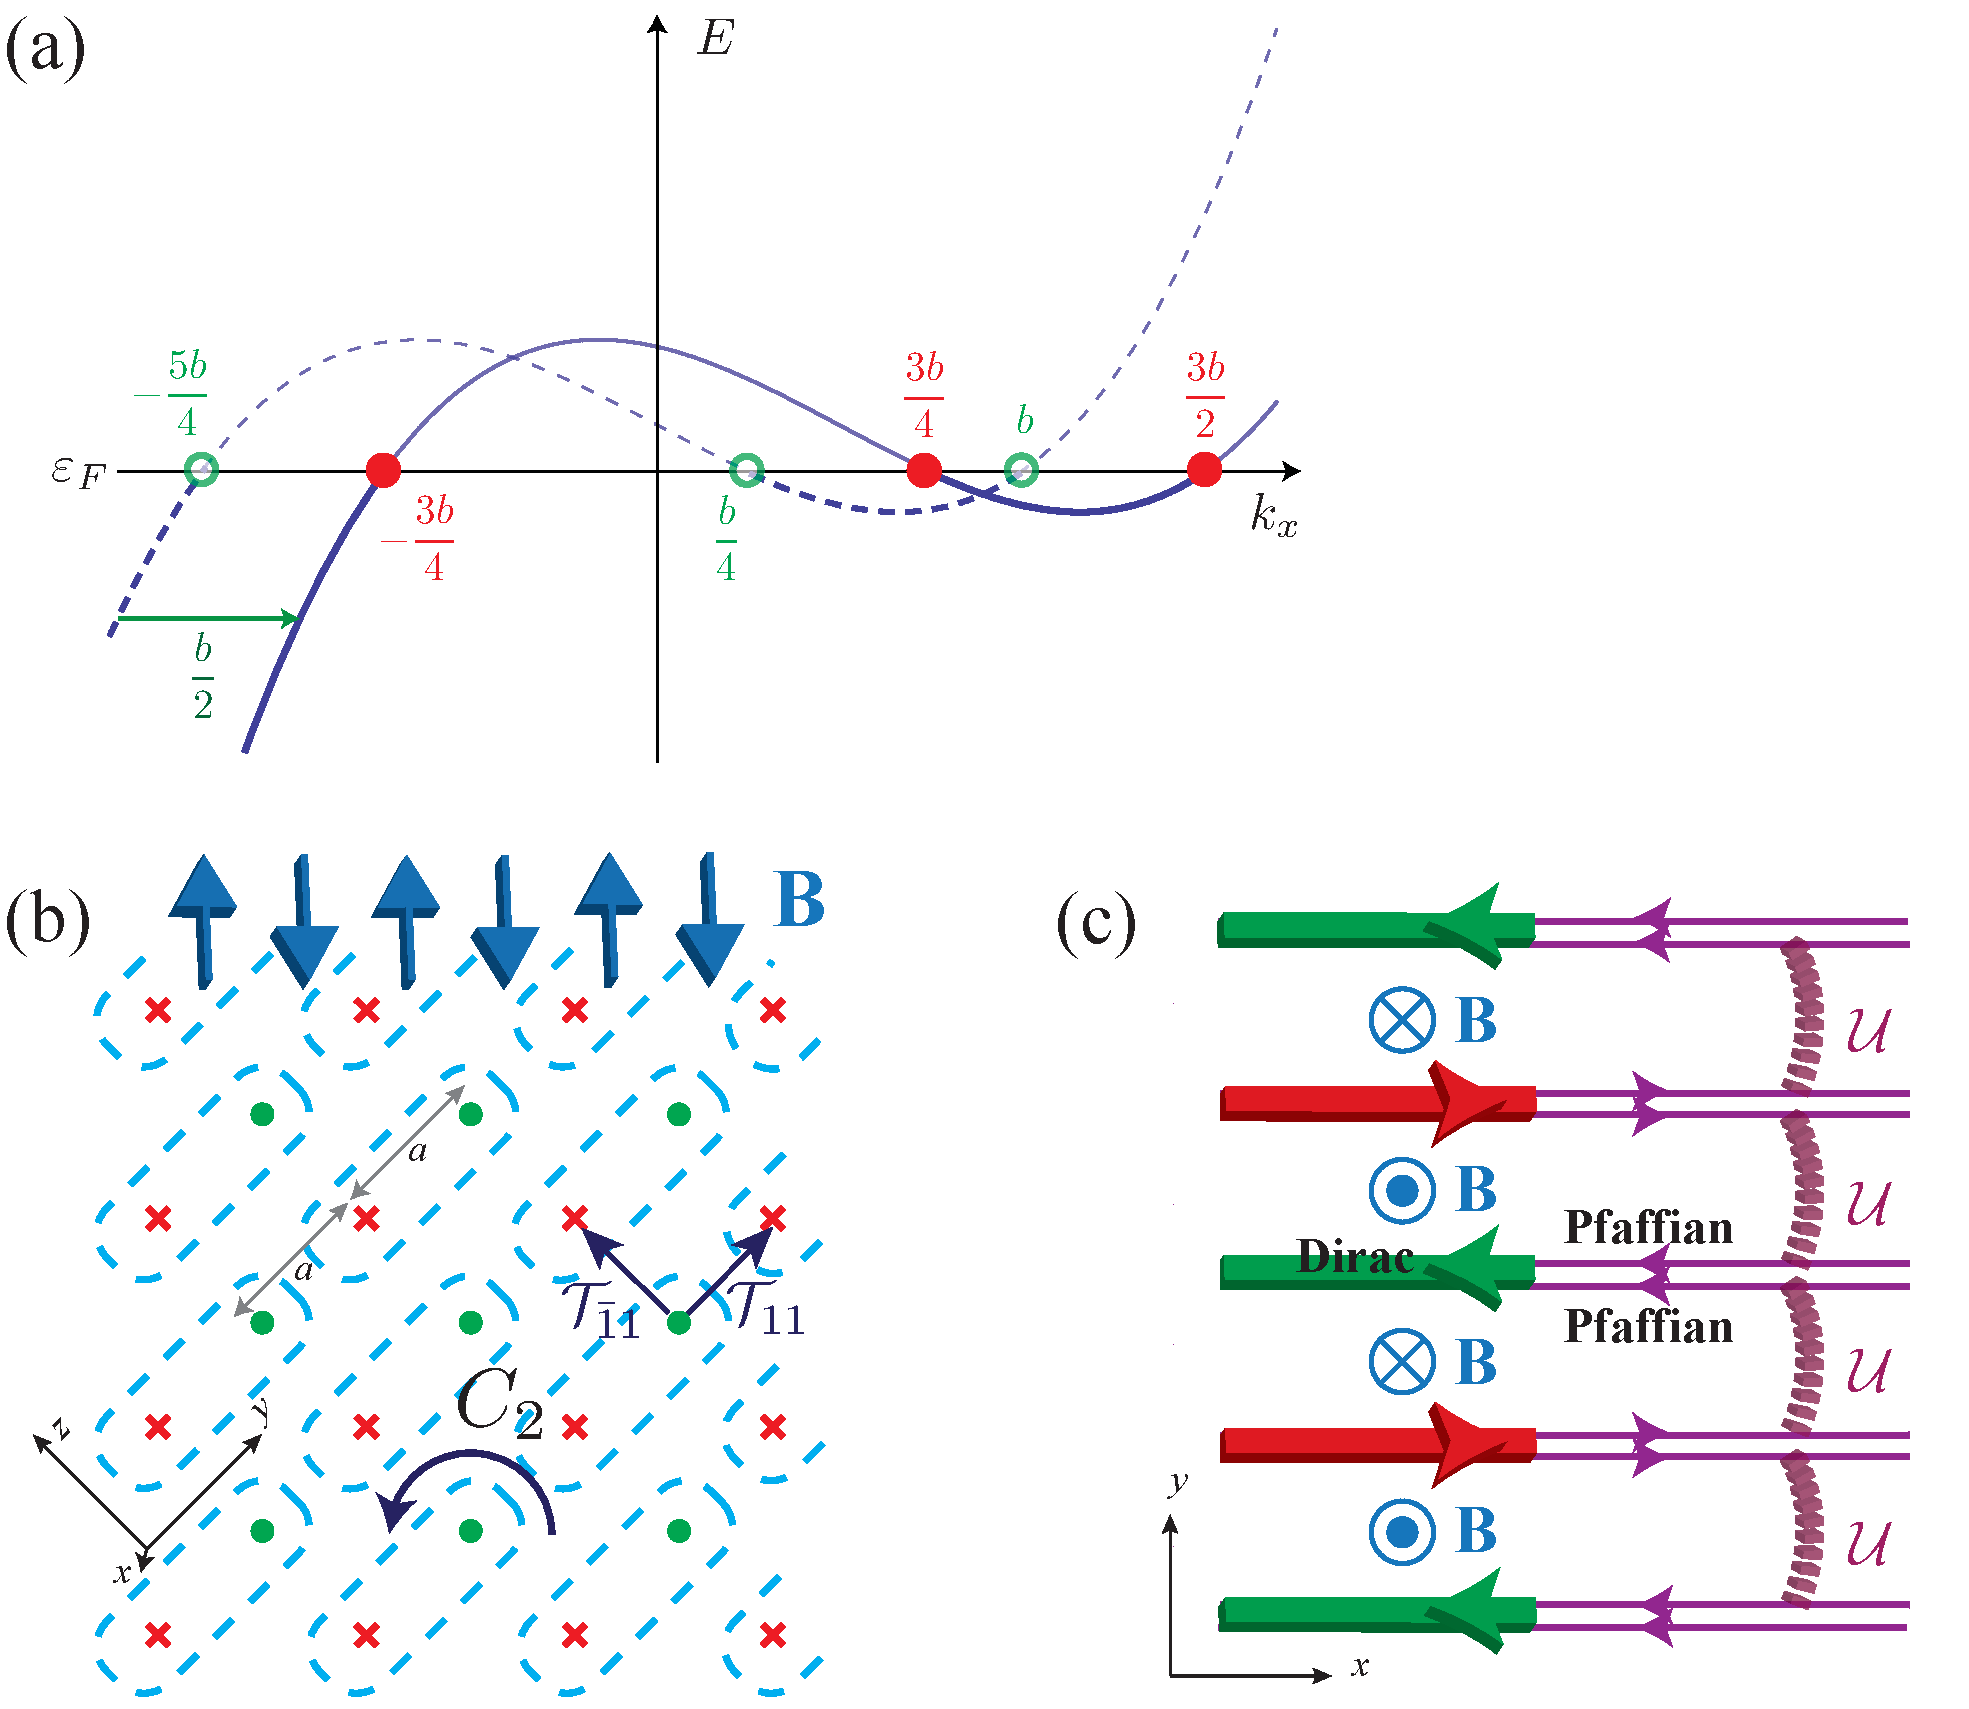
\includegraphics[width=0.45\textwidth]{afm}
\caption{(a) The energy dispersion $E_{y=2l}(k_x)$ with (solid curve) or without (dashed curve) the alternating magnetic field. (b) The alternating magnetic field configuration that preserves the AFTR and $C_2$ symmetries. (c) The alternating magnetic field across a single layer along the $xy$ plane.}\label{fig:afm}
\end{figure}

First we go back to a single Dirac wire and consider a non-linear dispersion \begin{align}E^0_{y=2l}(k_x)&=\frac{\hbar v}{b^2}(k_x-k_F^1)(k_x-k_F^2)(k_x-k_F^3),\nonumber\\E^0_{y=2l+1}(k_x)&=-\frac{\hbar v}{b^2}(k_x+k_F^1)(k_x+k_F^2)(k_x+k_F^3),\end{align} where $v$ and $b$ are some non-universal velocity and wave number parameters. We assume $k_F^2<k_F^3<k_F^1$ so that when the Fermi energy is at $\varepsilon_F=0$, there are two right (left) moving modes at $k_x=k_F^1,k_F^2$ and one left (resp.~right) moving one at $k_X=k_F^3$ along an even (resp.~odd) wire. This matches the three-channel Dirac wire \eqref{3Dirac} used in the splitting scheme in section~\ref{sec:gluing}. We assume the three Fermi wave numbers satisfy a commensurate condition \begin{align}2k_F^1+k_F^2-3k_F^3=0,\label{kcomm}\end{align} and we set \begin{align}b=2(k_F^3-k_F^1-k_F^2).\label{bcomm1}\end{align} The dashed band in figure~\ref{fig:afm}(a) shows one commensurate energy dispersion along an even wire.

Next, we consider a spatially modulating magnetic field ${\bf B}({\bf r})=B({\bf r}){\bf e}_{11}$, where \begin{align}B({\bf r})=\sum_{m=-\infty}^\infty B_m\sin\left[\pi\frac{\sqrt{2}(2m+1)}{a}{\bf e}_{\bar{1}1}\cdot{\bf r}\right],\end{align} ${\bf e}_{11}=({\bf e}_y+{\bf e}_z)/\sqrt{2}$ and ${\bf e}_{\bar{1}1}=(-{\bf e}_y+{\bf e}_z)/\sqrt{2}$, that preserves both the \AFTR and $C_2$ symmetries, \begin{align}B({\bf r}+a{\bf e}_y)=B({\bf r}+a{\bf e}_z)=B(C_2{\bf r})=-B({\bf r})\end{align} (see figure~\ref{fig:afm}(b) for the 3D field configuration). Moreover, we assume the field is commensurate with the Fermi wave numbers so that the magnetic flux per unit length across the $xy$ layer between adjacent wires (see figure~\ref{fig:afm}(c)) is \begin{align}\frac{\Phi_B}{L}=\frac{\phi_0}{2\pi}b\label{bcomm2}\end{align} where $L$ is the wire length, $\phi_0=hc/e$ is the magnetic flux quantum. Equivalently, the average magnetic field strength in the normal $z$-direction between adjacent wires is $|\overline{B_z}|=|\overline{B}|/\sqrt{2}=(\hbar c/ea)b$, where $a$ is the displacement between adjacent counter-propagating wires. We choose the vector potential $A_x(y,z)=[(-1)^y+(-1)^z-1]|\overline{B_z}|a/2$ and $A_y=A_z=0$ along the $(y,z)^{\mathrm{th}}$ wire. 

Along a wire on the $xy$ plane where $z=0$, the three electronic Dirac channels are now bosonized by \begin{align}\psi_y^{1,2}(x)&\sim e^{i[(-1)^y(k_F^{1,2}x+bx/2)+\tilde\phi_y^{1,2}(x)]},\\\psi_y^3(x)&\sim e^{i[(-1)^y(k_F^3x+bx/2)-\tilde\phi_y^3(x)]},\nonumber\end{align} where the momenta are shifted by $k_F^j\to k_F^j+(e/\hbar c)A_x$. The phase oscillation $e^{ikx}$ is canceled in an interaction term only when momentum is conserved, or otherwise the interaction would drop out after the integration over $x$. It is straightforward to check that the Majorana fermions \eqref{MFdef}, which contain the operators $e^{\pm i\phi^\sigma}$, have zero momentum because of the Fermi wave number commensurate condition \eqref{kcomm}. In addition, the boson backscattering $\cos(4\phi^A_{y+1}-4\phi^B_y)$ in \eqref{mbdint} preserves momentum because the magnetic field is also commensurate (see \eqref{bcomm1} and \eqref{bcomm2}).


\subsubsection{Interaction-enabled antiferromagnetic Dirac semimetal}\label{sec:intenable}
%Recall interaction enable topological phases
So far in this section, we have been discussing the gapping of the Dirac semimetal while preserving the \AFTR and $C_2$ symmetries. In this subsection, we focus on an opposite aspect of the symmetric many-body interaction -- the enabling of a (semi)metallic phase that is otherwise forbidden by symmetries in the single-body setting. We noticed in subsection~\ref{sec:anomaly} that the pair of momentum-separated Weyl points in figure~\ref{fig:Weylspectrum} is anomalous. In fact, it is well-known already that Weyl nodes~\cite{Murakami2007,WanVishwanathSavrasovPRB11,YangLuRan11,burkovBalenstPRL11,Ashvin_Weyl_review}, if separated in momentum space, must come in multiples of four in a lattice translation and time reversal symmetric three dimensional non-interacting system. 

This no go theorem can be rephrased into a feature. \begin{enumerate}\item If the low energy excitations of a time reversal symmetric lattice (semi)metal in three dimensions consists of one pair of momentum-separated Weyl nodes, then the system must involve many-body interaction.\end{enumerate} We refer to this time reversal and lattice translation symmetric strongly-correlated system as an interaction-enabled topological Dirac (semi)metal. We assume the Weyl nodes are fixed at two time reversal invariant momenta, and therefore they are stable against symmetry-preserving deformations. Otherwise, if the Weyl nodes are not located at high symmetry points, they can be moved and pair annihilated. Also, as explained in the beginning of section~\ref{sec:DiracSemimetal} and contrary to the more common contemporary terminology, we prefer to call the (semi)metal ``Dirac" rather than ``Weyl" because of the doubling. Perhaps more importantly, we propose the following conjecture. \begin{enumerate}\addtocounter{enumi}{1}\item Beginning with the interaction-enabled Dirac (semi)metal, {any} single-body symmetry-breaking mass must lead to a 3D gapped topological phase that cannot be adiabatically connected to a band insulator.\end{enumerate} We suspect this statement can be proven by a filling argument similar to that of Hasting-Oshikawa-Lieb-Schultz-Mattis~\cite{LiebSchultzMattis61,Oshikawa00,Hastings04}, and may already be available in Ref.~\onlinecite{WatanabePoVishwanath17} by Watanabe, Po and Vishwanath. This conjecture applies to the coupled wire situation where the gapped phase is long-range entangled and supports fractional excitations. Its topological order is out of the scope of this article, but will be presented in a future work~\cite{SirotaRazaTeoappearsoon}. In a broader perspective, this type of statements may provide connections between strongly-interacting and non-interacting phases and help understanding quantum phase transitions of long-range entangled 3D phases from that of single-body band insulating ones.

Before discussing the three dimensional case, we make the connection to a few known interaction-enabled topological phases with or without an energy gap in low dimensions. First, zero energy Majorana fermions $\gamma_j=\gamma_j^\dagger$ in a true zero dimensional non-interacting (spinless) time reversal symmetric system must bipartite into an equal number of positive chiral ones $\mathcal{T}\gamma_j\mathcal{T}^{-1}=+\gamma_j$ and negative chiral ones $\mathcal{T}\gamma_l\mathcal{T}^{-1}=-\gamma_l$. Fidkowski and Kitaev showed in Ref.~\onlinecite{FidkowskiKitaev10} that under a combination of two-body interactions, eight Majoranas with the same chirality can acquire a time reversal preserving mass and be removed from low energy. This leaves behind a collection of zero energy Majoranas that have a non-trivial net chirality of eight. Second, all $(1+1)$D time reversal symmetric topological BDI superconductors~\cite{SchnyderRyuFurusakiLudwig08,Kitaevtable08,QiHughesRaghuZhang09,HasanKane10,QiZhangreview11,RMP} must break inversion because the zero energy Majorana boundary modes must have opposite chiralities at opposite ends. The Fidkowski-Kitaev interaction however allows one to construct a non-trivial $(1+1)$D topological model that preserves both time reversal and inversion but at the same time supports four protected Majorana zero modes at each end~\cite{LapaTeoHughes14}. Third, a single massless Dirac fermion in $(2+1)$D is anomalous in a (spinful) time reversal and charge $U(1)$ preserving non-interacting lattice system. On the other hand, it can be enabled by many-body interactions. For instance, when one of the two opposing surfaces of a topological insulator slab is gapped by symmetry-preserving interactions~\cite{WangPotterSenthilgapTI13,MetlitskiKaneFisher13b,ChenFidkowskiVishwanath14,BondersonNayakQi13}, a single massless Dirac fermion is left behind on the opposite surface as the only gapless low energy degrees of freedom of the quasi-$(2+1)$D system. Similar slab construction can be applied to the superconducting case, and interactions can allow any copies of massless Majorana fermions to manifest in $(2+1)$D with the presence of (spinful) time reversal symmetry.

On the contrary, there are anomalous gapless fermionic states that cannot be enabled even by strong interactions. Chiral fermions that only propagate in a single direction cannot be realized in a true $(1+1)$D lattice system. They can only be supported as edge modes of $(2+1)$D topological phases such as quantum Hall states~\cite{Wenedgereview} or chiral $p_x+ip_y$ superconductors~\cite{Volovik99,ReadGreen}. Otherwise, they would allow heat transfer~\cite{KaneFisher97,Cappelli01,Kitaev06} from a low temperature reservoir to a high temperature one, thereby violating the second law of thermodynamics. Similarly, a single massless Weyl fermion can only be present as the $(3+1)$D boundary state of a $(4+1)$D topological bulk~\cite{ZhangHu01,BernevigChernHuToumbasZhang02,QiHughesZhang08,SchnyderRyuFurusakiLudwig08,Kitaevtable08}. It cannot exist in a true $(3+1)$D lattice system~\cite{Nielsen_Ninomiya_1981,NielsenNinomiyaPLB1981}, or otherwise under a magnetic field there would be unbalanced chiral fermions propagating along the field direction that constitute the ABJ-anomaly~\cite{Adler69,BellJackiw69,NielsenNinomiya83}.

\begin{figure}[htbp]
\centering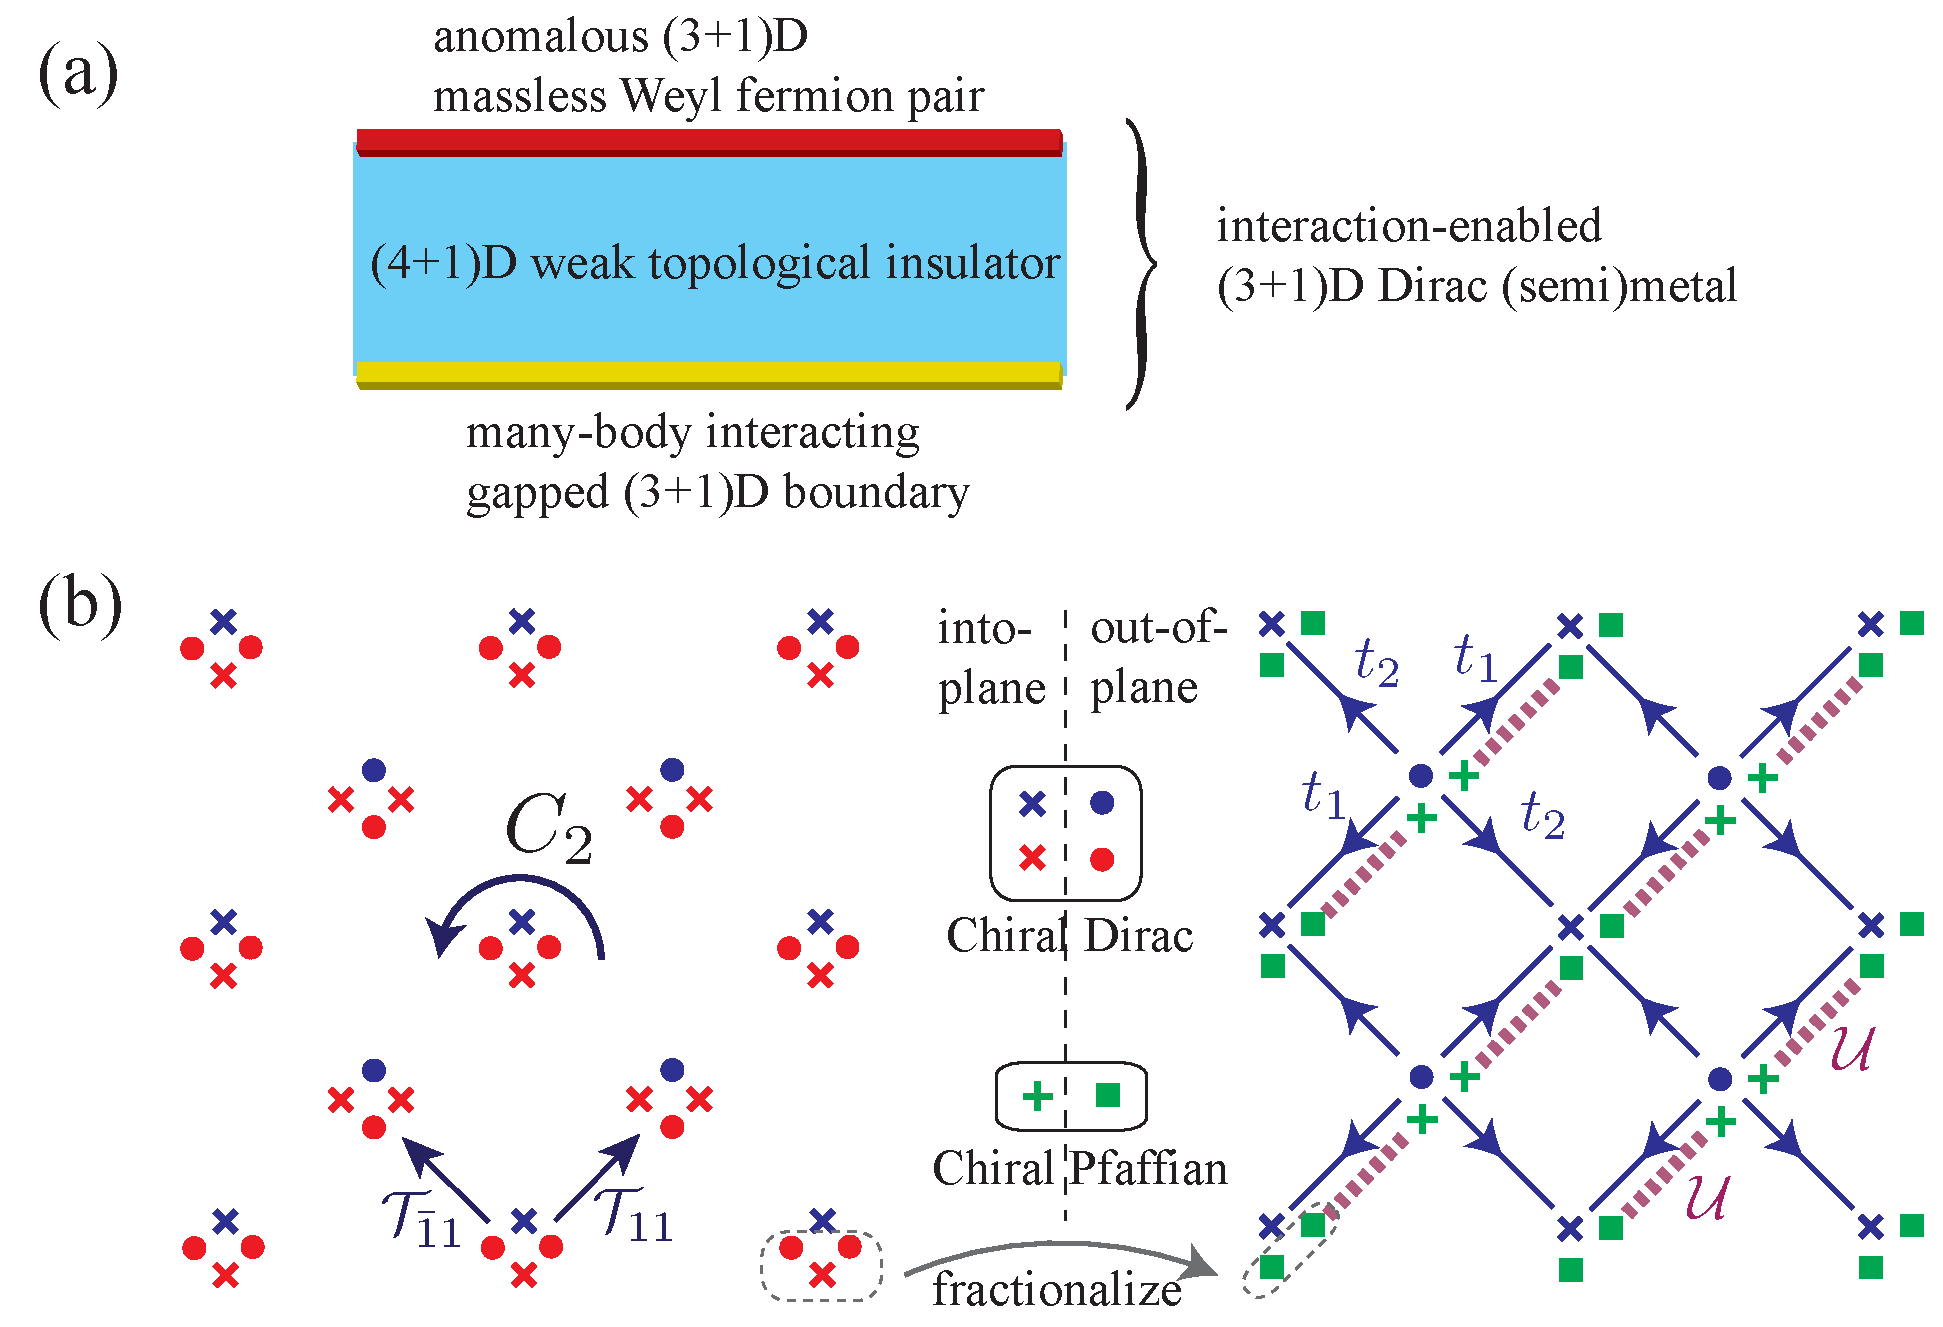
\includegraphics[width=0.47\textwidth]{intenable}
\caption{(a) A quasi-$(3+1)$D interaction-enabled Dirac (semi)metal constructed by a 4D slab of WTI. (b) Coupled wire model of an anomalous Dirac (semi)metal enabled by interaction with $C_2$ rotation and both AFTR $\mathcal{T}_{11},\mathcal{T}_{\bar{1}1}$ symmetries.}\label{fig:intenable}
\end{figure}

In this section, we focus on the simplest anomalous gapless fermionic states in $(3+1)$D that can be enabled by interactions. As eluded in section~\ref{sec:holproj4D}, a weak topological insulator in $(4+1)$D can support the anomalous energy spectrum in figure~\ref{fig:Weylspectrum} on its boundary so that a pair of opposite Weyl points sit at two distinct time reversal invariant momenta on the boundary Brillouin zone. A 4D weak topological insulator slab, where the fourth spatial dimension is open and the other three are periodic, has two $(3+1)$D boundaries and each carries a pair of Weyl fermions. The coupling between the two pairs of Weyl fermions are suppressed by the system thickness and bulk energy gap. By introducing symmetry-preserving gapping interactions on the bottom surface, the anomalous gapless fermionic state is left behind on the top surface and is enabled in this quasi-$(3+1)$D setting (see figure~\ref{fig:intenable}(a)).

Inspired by this construction, we propose a true $(3+1)$D coupled wire model which has the the anomalous energy spectrum in figure~\ref{fig:Weylspectrum} and preserves the \AFTR symmetries in both $\mathcal{T}_{11}$ and $\mathcal{T}_{\bar{1}1}$ directions as well as the $C_2$ (screw) rotation symmetry. The model is summarized in figure~\ref{fig:intenable}(b). It consists of a checkerboard array of electronic wires, where each wire has two chiral Dirac channels propagating into-paper and another two propagating out-of-paper. Contrary to the model considered in section~\ref{sec:DiracSemimetal}, here the net chirality on each wire cancels and therefore the wires are true $(1+1)$D systems without being supported by a higher dimensional bulk. Using the splitting scheme described in section~\ref{sec:gluing}, along each wire, one can fractionalize a group of three Dirac channels {\color{red}$\bullet\bullet\times$} ({\color{red}$\times\times\bullet$}) into a pair of co-propagating chiral Pfaffian channels {\color{green}$\blacksquare\blacksquare$} (resp.~{\color{green}$++$}). The two Pfaffian channels then can be backscattered in opposite directions using the many-body interaction $\mathcal{U}$ (dashed purple lines) described in section~\ref{sec:interactionmodels}. This introduces an excitation energy gap that removes three Dirac channels per wire from low energy. Lastly, single-body backscatterings $t_1,t_2$ (solid directed blue lines) among the remaining Dirac channels {\color{blue}$\bullet\times$} described in \eqref{WeylTBHam} and figure~\ref{fig:WeylTB} give rise to the low-energy Weyl spectrum in figure~\ref{fig:Weylspectrum}. Since the many-body interaction $\mathcal{U}$ and the single-body backscatterings $t_1,t_2$ preserve the $C_2$ rotation and both \AFTR symmetries $\mathcal{T}_{11}$ and $\mathcal{T}_{\bar{1}1}$, the model describes an interaction-enabled anomalous (semi)metal that is otherwise forbidden in a non-interacting non-holographic setting. 

The non-local anti-ferromagnetic nature of the time reversal symmetry is built-in in the present coupled wire model. We speculate in passing that a local conventional time reversal symmetric Dirac (semi)metallic phase consisting of a single pair of momentum-space-separated Weyl nodes may also be enabled by interaction. On one hand, the \AFTR symmetry could be restored to a local time reversal symmetry by ``melting" the checkerboard wire array. On the other hand, there could also be an alternative wire configuration that facilitates a coupled wire model with a local conventional time reversal symmetry.

Lastly, we gap the interaction-enabled Dirac semimetallic model (figure~\ref{fig:intenable}) by a symmetry-breaking single-body mass. This can be achieved by introducing electronic backscattering terms that dimerize the remaining Dirac channels {\color{blue}$\bullet\times$}, and were described by \eqref{DiracTBHam} in section~\ref{sec:brokensymmetry}. The resulting state is an insulating $(3+1)$D topological phase with long-range entanglement. For instance, each diagonal layer gapped by the many-body interaction $\mathcal{U}$ has the identical topological order of the $\mathcal{T}$-Pfaffian surface state of a topological insulator. 

\subsubsection{Fractional surface states}\label{sec:fracsurface}

In section~\ref{sec:fermiarcAFTRpreserving} and ~\ref{sec:fermiarcAFTRbreaking}, we discussed the surface states of the single-body coupled Dirac wire model \eqref{WeylTBHam} (see also figure~\ref{fig:WeylTB}). In particular, we showed in figure~\ref{fig:SurfaceStates1bdy} that an \AFTR symmetry preserving surface hosts open chiral Dirac channels, which connect and leak into the 3D (semi)metallic bulk. Earlier in this section, we discussed the effects of many-body interaction, which leads to two possible phases: (a) a gapped topological phase (see section~\ref{sec:interactionmodels}) that preserves one of the two \AFTR symmetries, say $\mathcal{T}_{11}$, and (b) a gapless interaction-enabled Dirac semimetal (see section~\ref{sec:intenable}) that preserves the $C_2$ rotation and both \AFTR symmetries $\mathcal{T}_{11}$ and $\mathcal{T}_{\bar{1}1}$. Here, we describe the boundary states of the two interacting phases on a surface closed under the symmetries.

\begin{figure}[htbp]
\centering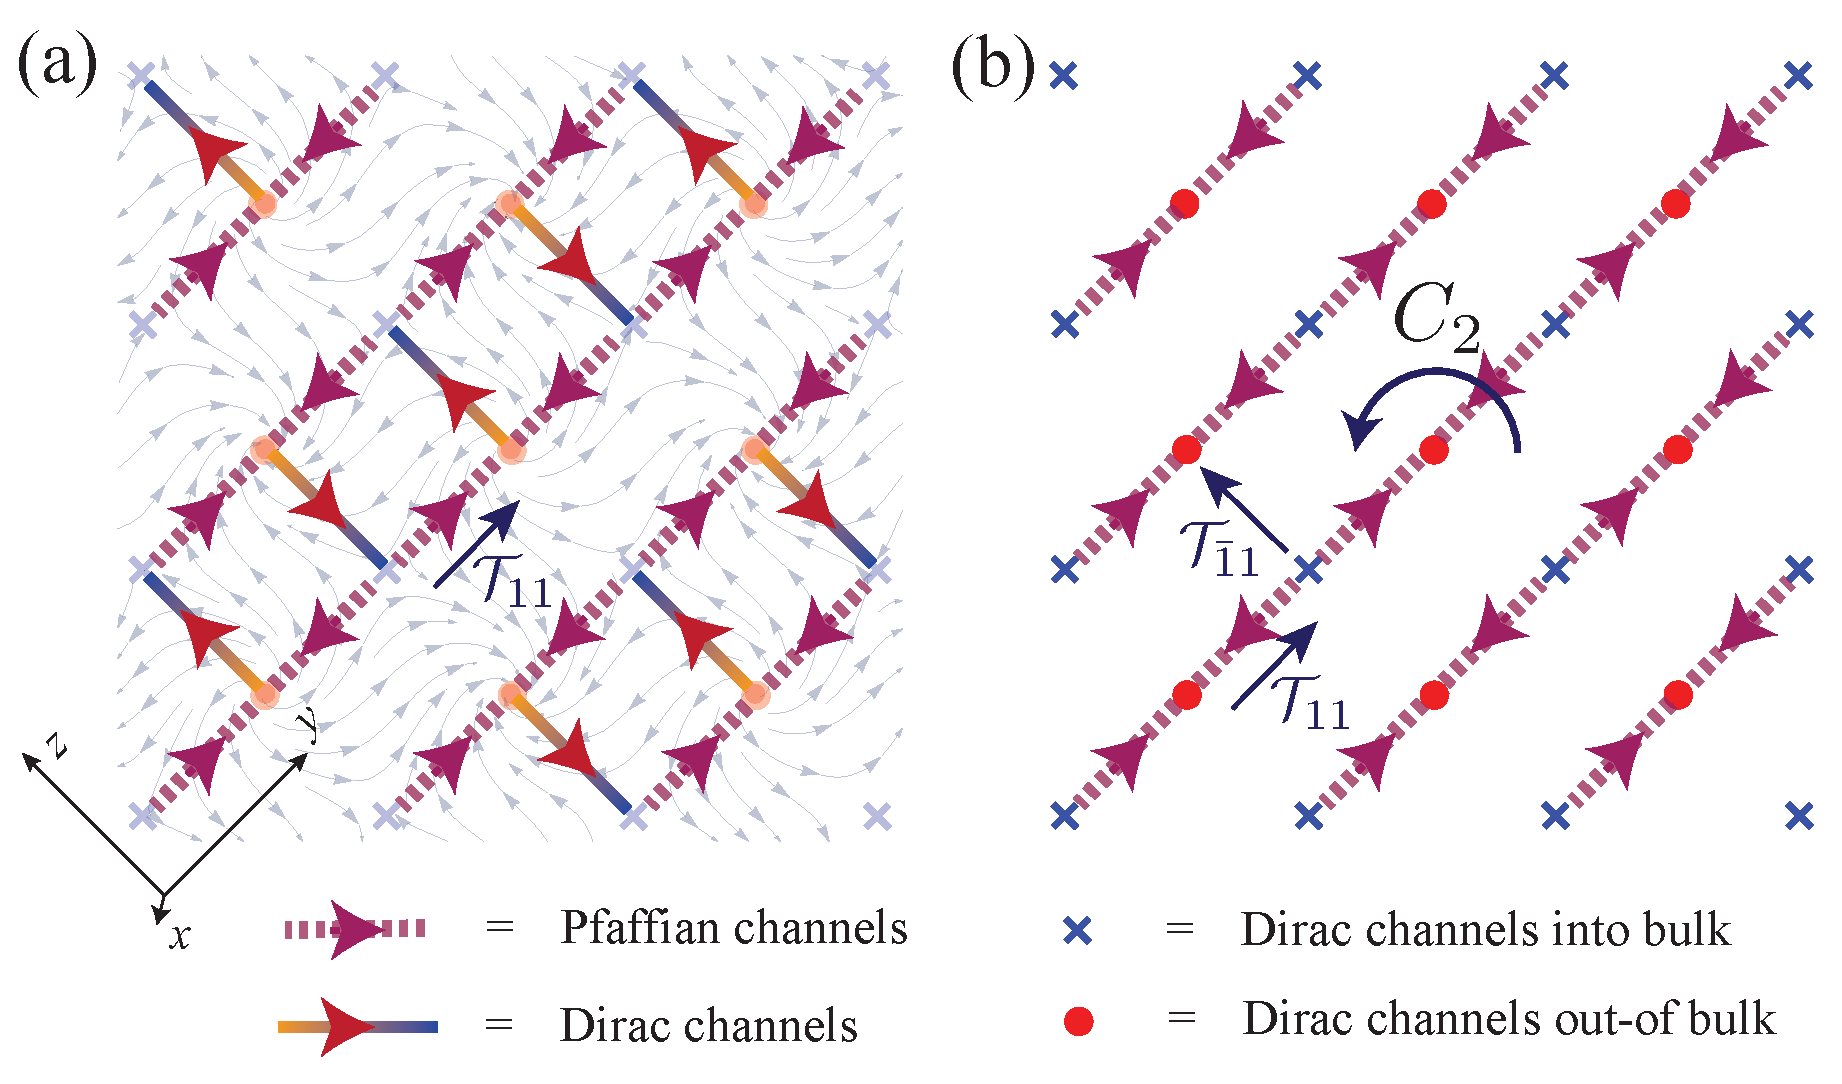
\includegraphics[width=0.48\textwidth]{SurfaceStates}
\caption{Fractional surface states of (a) a 3D Dirac insulator gapped by many-body interaction that preserves $\mathcal{T}_{11}$, and (b) a 3D gapless interaction-enabled Dirac semimetal that preserves $\mathcal{T}_{11}$, $\mathcal{T}_{\bar{1}1}$ and $C_2$.}\label{fig:SurfaceStates}
\end{figure}

First, we consider the coupled wire model with the many-body interaction \eqref{mbdint} (see also figure~\ref{fig:gappinginteraction}) and a boundary surface along the $yz$-plane perpendicular to the wires. The surface network of fractional channels is shown in figure~\ref{fig:SurfaceStates}(a). We assume the bulk chiral Dirac wires ({\color{blue}$\times$}{\color{red}$\bullet$}) are supported as vortices of Dirac mass in the bulk (recall \eqref{DiracHam}), where the texture of the mass parameters is represented by the underlying vector field. The model is juxtaposed along the $yz$- boundary plane against the trivial Dirac insulating state $H_{\mathrm{vacuum}}=\hbar v{\bf k}\cdot\vec{s}\mu_z+m_0\mu_x$, which models the vacuum. The line segments on the surface plane where the Dirac mass $m_0\mu_x$ changes sign host chiral Dirac channels (c.f.~subsection~\ref{sec:fermiarcAFTRpreserving}).

Unlike the single-body (semi)metallic case in figure~\ref{fig:SurfaceStates1bdy} where the surface Dirac channels connects with the bulk ones, now the many-body interacting bulk is insulating and does not carry low-energy gapless excitations. Thus, the surface Dirac channels here cannot leak into the bulk and must dissipate to other low-energy degrees of freedom on the surface. The many-body interwire backscattering interaction in \eqref{mbdint} (and figure~\ref{fig:gappinginteraction}) leaves behind chiral Pfaffian channels on the surface. These fractional channels connect back to the surface Dirac channels in pairs. The surface network of chiral channels preserves the \AFTR $\mathcal{T}_{11}$ symmetry. However, the low-energy surface state is not protected. Electronic states can be localized by dimerizing the Pfaffian channels in the $z$ (or $\bar{1}1$) direction.

Second, we consider the interaction-enabled Dirac semimetallic model summarized in figure~\ref{fig:intenable}(b) in section~\ref{sec:intenable} and again let it terminate along the symmetry preserving $yz$-plane perpendicular to the wires. The surface gapless channels are shown in figure~\ref{fig:SurfaceStates}(b). Here, the semimetallic bulk preserves $C_2$ as well as the two \AFTR symmetries $\mathcal{T}_{11}$ and $\mathcal{T}_{\bar{1}1}$. The bulk array of wires are true $(1+1)$D systems and are not supported as edge modes or vortices of a higher dimensional bulk. The pair of into-paper Dirac modes are bent into the pair of out-of-paper ones along each wire at the terminal. Similar to the previous case, the many-body bulk interwire backscattering interaction leaves behind surface chiral Pfaffian channels. Through the mode bending at the wire terminal, these Pfaffian channels join in pairs and connect to the chiral Dirac channels in the bulk that constitute the Dirac semimetal. In this case, the surface state is protected by $C_2$, $\mathcal{T}_{11}$ and $\mathcal{T}_{\bar{1}1}$, and is forced to carry fractional gapless excitations as a consequence and signature of the anomalous symmetries. For instance, the charge $e/4$ Ising-like quasiparticle and the charge $e/2$ semion can in principle be detected by shot noise tunneling experiments. These gapless fractional excitations however are localized on the surface because the Dirac (semi)metallic bulk only supports gapless electronic quasiparticles.




\subsection{Conclusion and Discussion}
Dirac and Weyl (semi)metals have generated immense theoretical and experimental interest. On the experimental front, this is fueled by an abundant variety of material classes and their detectable \ARPES and transport signatures. On the theoretical front, Dirac/Weyl (semi)metal is the parent state that, under appropriate perturbations, can give birth to a wide range of topological phases, such as topological (crystalline) insulators and superconductors. In this work, we explored the consequences of a specific type of strong many-body interaction based on a coupled-wire description. In particular, we showed that (i) a 3D Dirac fermion can acquire a finite excitation energy gap in the many-body setting while preserving the symmetries that forbid a single-body Dirac mass, and (ii) interaction can enable an anomalous antiferromagnetic time-reversal symmetric topological (semi)metal whose low-energy gapless degrees of freedom are entirely described by a pair of non-interacting electronic Weyl nodes separated in momentum space. A brief conceptual summary was presented in section~\ref{sec:introsummary} and will not be repeated here. Instead, we conclude by discussing possible future directions.

%superconducting version and nodal systems
First, coupled wire constructions can also be applied in superconducting settings and more general nodal electronic systems. For example, a Dirac/Weyl metal can be turned into a topological superconductor~\cite{SchnyderRyuFurusakiLudwig08,Kitaevtable08,QiHughesRaghuZhang09} under appropriate intra-species (i.e.~intra-valley) $s$-wave pairing~\cite{QiWittenZhang13}. Pairing vortices host gapless chiral Majorana channels~\cite{QiWittenZhang13,GuQi15,LopesTeoRyu17}. An array of these chiral vortices can form the basis in modeling superconducting many-body topological phases in three dimensions. On the other hand, instead of considering superconductivity in the continuous bulk, inter-wire pairing can also be introduced in the coupled Dirac wire model and lead to new topological states~\cite{ParkTeoGilbertappearsoon}.

Dirac/Weyl (semi)metals are a specific type of nodal electronic matter. For example, nodal superconductors were studied in states with dx$^2$-y$^2$ pairing~\cite{RyuHatsugaiPRL02}, He$^3$ in its superfluid A-phase~\cite{Volovik3HeA,Volovikbook}, and non-centrosymmetric states~\cite{SchnyderRyuFlat,BrydonSchnyderTimmFlat}. Weyl and Dirac fermions were generalized in time reversal and mirror symmetric systems to carry $\mathbb{Z}_2$ topological charge~\cite{morimotoFurusakiPRB14}. General classification and characterization of gapless nodal semimetals and superconductors were proposed~\cite{Sato_Crystalline_PRB14,ZhaoWangPRL13,ZhaoWangPRB14,ChiuSchnyder14,matsuuraNJP13,Volovikbook,RMP,HoravaPRL05}. It would be interesting to investigate the effect of strong many-body interactions in general nodal systems.

Second, in section~\ref{sec:DiracSemimetal}, we described a coarse-graining procedure of the coupled wire model that resembles a real-space renormalization and allows one to integrate out high energy degrees of freedom. While this procedure was not required in the discussions that follow because the many-body interacting model we considered was exactly solvable, it may be useful in the analysis of generic interactions and disorder. The coarse-graining procedure relied on the formation of vortices, which were introduced extrinsically. Like superconducting vortices, it would be interesting as a theory and essential in application to study the mechanism where the vortices of Dirac mass can be generated dynamically. To this end, it may be helpful to explore the interplay between possible (anti)ferromagnetic orders and the spin-momentum locked Dirac fermion through antisymmetric exchange interactions like the Dzyaloshinskii-Moriya interaction~\cite{Dzyaloshinsky58,Moriya60}.

%topological order, threefold lattice and alternative fractionalization
Third, the symmetry-preserving many-body gapping interactions considered in section~\ref{sec:interaction} have a ground state that exhibits long-range entanglement. This entails degenerate ground states when the system is compactified on a closed three dimensional manifold, and fractional quasi-particle and quasi-string excitations or defects. These topological order properties were not elaborated in our current work but will be crucial in understanding the topological phase~\cite{SirotaRazaTeoappearsoon} as well as the future designs of detection and observation. It would also be interesting to explore possible relationships between the coupled wire construction and alternative exotic states in three dimensions, such as the Haah's code~\cite{Haah11,Haah13}.

Fourth, the many-body inter-wire backscatterings proposed in section~\ref{sec:interactionmodels} were based on a fractionalization scheme described in \ref{sec:gluing} that decomposes a chiral Dirac channel with $(c,\nu)=(1,1)$ into a decoupled pair of Pfaffian ones each with $(c,\nu)=(1/2,1/2)$. In theory, there are more exotic alternative partitions. For instance, if a Dirac channel can be split into three equal parts instead of two, an alternative coupled wire model that put Dirac channels on a honeycomb vortex lattice could be constructed by backscattering these fractionalized channels between adjacent pairs of wires. Such higher order decompositions may already be available as conformal embeddings in the conformal field theory context. For example, the affine $SU(2)$ Kac-Moody theory at level $k=16$ has the central charge $c=8/3$, and its variation may serve as the basis of a "ternionic" model.

%Continuum model
%Material realization?
%Melting
%Defect modes
%Linear response theory
\section{Surfaces and Slabs of Fractional Topological Insulator Heterostructures}
%\documentclass[aps,prb,reprint,twocolumn,superscriptaddress,floatfix,10pt,letterpaper,showpacs]{revtex4-1}
%\usepackage{amsmath,amssymb,amsfonts,stmaryrd,wasysym,graphicx,multirow,color,textcomp}
%\usepackage{url}%\usepackage{diagrams}
%\usepackage[colorlinks=true,citecolor=blue,urlcolor=blue]{hyperref}

\newcommand{\TPf}{\hyperlink{TPf}{$\mathcal{T}$-$\mathrm{Pf}^\ast$} }


\subsection{\label{sec:Intro}Introduction}
Conventional topological insulators (\hypertarget{TI}{TI})~\cite{FuKaneMele3D,Roy07,MooreBalents07,QiHughesZhang08} are time reversal and charge $U(1)$ symmetric electronic band insulators in three dimensions that host massless surface Dirac fermions. The topologically protected surface Dirac fermion can acquire a single-body ferromagnetic or superconducting mass by breaking time reversal or charge $U(1)$ symmetry respectively, as described in the introduction chapter. Alternatively it can acquire a many-body interacting mass while preserving both symmetries, and exhibit long-ranged entangled surface topological order~\cite{WangPotterSenthilgapTI13,MetlitskiKaneFisher13b,ChenFidkowskiVishwanath14,BondersonNayakQi13}. Interfaces between different massive surface domains host exotic massless quasi-$(1+1)$D electronic channels~\cite{TeoKane,FuKanechargetransport09,QiWittenZhang13}, and consequently, from the bulk-boundary correspondence, topological insulator slabs with distinct gapped surface orders lead to a variety of quasi-$(2+1)$D topological phases. 
On the other hand, fractional topological insulators (\hypertarget{FTI}{FTI})~\cite{MaciejkoQiKarchZhang10,SwingleBarkeshliMcGreevySenthil11,maciejko2012models,ye2016composite,maciejko2015fractionalized,stern2016fractional,YeChengFradkin17} are long-range entangled topologically ordered electronic phases in $(3+1)$ dimensions outside of the single-body mean-field band theory description. They carry fractional quasi-particle and quasi-string excitations that cannot be adiabatically connected to the electron. 
They carry time reversal and charge $U(1)$ symmetries, which enrich its topological order (local excitation spectrum) in the sense that a symmetric surface must be anomalous and cannot be realized non-holographically by a true $(2+1)$-D system. In this paper, we describe the topological properties of various massive surface states and quasi-$(2+1)$-D slabs of a series of a fractional topological insulator. In particular, we focus on the quasi-particle structure.

\begin{figure}[htbp]
\centering\includegraphics[width=0.9\textwidth]{fig1}
%\caption{Summary of the \QP and gauge flux content in \FTI slabs. A pair of $\mathrm{Pf}^\ast$ \FTI slabs are merged into a fracional Chern \FTI slab $\mathcal{F}$ by gluing the two \TR symmetric \TPf surfaces. Directed bold lines on the front surfaces are chiral edge modes of the $\mathrm{Pf}^\ast$ and $\mathcal{F}$ \FTI slabs.}\label{fig1}
\caption{Summary of the quasiparticle and gauge flux content in fractional topological insulator slabs. A pair of $\mathrm{Pf}^\ast$ fractional topological insulator slabs are merged into a fractional Chern insulator slab $\mathcal{F}$ by gluing the two time reversal symmetric $\mathcal{T}$-$\mathrm{Pf}^\ast$ surfaces. Directed bold lines on the front surface are chiral edge modes of the $\mathrm{Pf}^\ast$ and $\mathcal{F}$ fractional topological insulator slabs.}\label{fig1}
\end{figure}

We focus on a series of fermionic fractional topological insulators, labeled by integers $n$, whose magneto-electric response is characterized by the $\theta$-angle $\theta=\pi/(2n+1)$ (modulo $2\pi/(2n+1)$) that associates an electric charge of $e^\ast/2=e/2(2n+1)$ to each magnetic monopole~\cite{Witten79}, for $e$ the electric charge of the electron. In particular, we consider fractional topological insulators that support deconfined fermionic parton excitations $\psi$ in the bulk, each carrying a fractional electric charge of $e^\ast=e/(2n+1)$. This assumes the electron can be written as 2n+1 parts, i.e.  $\psi_{\mathrm{el}}\sim\psi_1\ldots\psi_{2n+1}$. The $(3+1)$-D topological order is based on a discrete $\mathbb{Z}_{2n+1}$ gauge theory~\cite{maciejko2012models}. This is necessary because these particles do not exist outside of the insulator, and so must glue together. This gauge theory ensures that, and there are several ways to do this but we just consider one.  The theory supports electrically neutral string-like gauge flux $\Phi$, so that a monodromy quantum phase of $e^{2\pi ig/(2n+1)}$ is obtained each time $\psi$ orbits around it. In other words, $\psi$ carries the gauge charge $g$ that braids with the gauge flux. The integer $g$ and $2n+1$ are relatively prime so that all local quasiparticles be combinations of the electronic quasiparticles $\psi_{\mathrm{el}}$ and hence must carry integral electric charges and trivial gauge charges.

Generalizing the surface state of a conventional topological insulator, the surface of a fractional topological insulator hosts massless Dirac partons coupling with a $\mathbb{Z}_{2n+1}$ gauge theory. These anyons are bosons. Unlike its non-interacting counterpart whose gapless Dirac surface state is symmetry protected in the single-body picture, a fractional topological insulator is strongly interacting to begin with and there is no topological reason for its surface state to remain gapless. In this paper we focus on three types of gapped surface states -- ferromagnetic surfaces that break time reversal, superconducting surfaces that break charge $U(1)$, and symmetric surfaces which generalize the $\mathcal{T}$-Pfaffian surface state of a conventional topological insulator and is denoted by {$\mathcal{T}$-$\mathrm{Pf}^\ast$}. The topological order for fractional topological insulator slab with these surfaces are discussed in Sec.~\ref{FS}, \ref{SCS} and \ref{TPF} respectively. In Sec.~\ref{Gluing}, we discuss, using an anyon condensation picture, the gluing of a pair of $\mathcal{T}$-Pfaffian surfaces. We conclude in Sec.~\ref{Conclusion} with remarks on a complementary way to understand these topological order \cite{ChoTeoFradkin17}.
\subsection{\label{FS}Ferromagetic Heterostructure}
We begin with a slab that has opposite time reversal breaking ferromagnetic surfaces. In the ferromagnetic surfaces, in addition to the single-body Dirac mass $m$ for the surface parton, the $\mathbb{Z}_{2n+1}$ gauge sector also shows a time reversal breaking signature. The $\mathbb{Z}_{2n+1}$ gauge theory is only present inside the fractional topological insulator, and when a flux line $\Phi$ terminates at the surface, the time reversal breaking boundary condition confines an electrically neutral surface gauge quasiparticle, denoted by $\zeta^a$, with gauge charge $a$ at the flux-surface junction (see Fig.~\ref{fig1}). This gauge flux-charge composite, referred to as a dyon $\delta=\Phi\times\zeta^a$, carries fractional spin $h_\delta=a/(2n+1)$ because a $2\pi$-rotation about the normal axis braids $a$ gauge charges around $\Phi$ and results in the monodromy quantum phase of $e^{2\pi ia/(2n+1)}$. Time reversal conjugates all quantum phases so, $a\not\equiv0$ modulo $2n+1$ breaks time reversal.

The one-dimensional interface between two time reversal conjugate ferromagnetic surface domains hosts a fractional chiral channel. For example, the interface between two ferromagnetic domains with opposite ferromagnetic orientations on the surface of a conventional topological insulator bounds a chiral Dirac channel~\cite{TeoKane,FuKanechargetransport09,QiWittenZhang13}, where electrons propagate only in the forward direction. Alternatively, a topological insulator slab with opposite time reversal breaking ferromagnetic surfaces is topologically identical to a quasi-$(2+1)$-D Chern insulator~\cite{Haldane1988,liu2016quantum} and supports a chiral Dirac edge mode. Similarly, in the fractional topological insulator case, the low-energy content of the fractional chiral channel between a pair of time reversal conjugate ferromagnetic surface domains can be inferred by the edge mode of a fractional topological insulator slab with time reversal breaking ferromagnetic surfaces that is topologically identical to a quasi-$(2+1)$-D fractional Chern insulator~\cite{RegnaultBernevigfractionchern,NeupertSantosChamonMudry11,TangMeiWen11,ShengGuSunSheng11} or fractional quantum Hall (\hypertarget{FQH}{FQH}) state~\cite{FQHE_Review}. The chiral $(1+1)$-D channel is characterized by two response quantities~\cite{Laughlin_IQHE, Halperin82, Hatsugai93, Schulz00, Volovik92, KaneFisher97, Cappelli01, Kitaev06, Luttinger64} -- the differential electric conductance $\sigma=dI/dV=\nu e^2/h$ that relates the changes of electric current and potential, and the differential thermal conductance $\kappa=dI_T/dT=c(\pi^2k_B^2/3h)T$ that relates the changes of energy current and temperature. In the slab geometry, they are equivalent to the Hall conductance $\sigma=\sigma_{xy}$, $\kappa=\kappa_{xy}$. $\nu=N_e/N_\phi$ is also referred to as the filling fraction of the fractional topological insulator slab and associates the gain of electric charge (in units of $e$) to the addition of a magnetic flux quantum $hc/e$. $c=c_R-c_L$ is the chiral central charge of the conformal field theory (\hypertarget{CFT}{CFT})~\cite{bigyellowbook} that effectively describes the low-energy degrees of freedom of the fractional chiral channel. 

Since the top and bottom surfaces of the fractional topological insulator slab are time reversal conjugate, their parton Dirac masses $m$ and gauge flux-charge ratio $a$ have opposite signs. The anyon content is generated by the partons and gauge dyons. When a gauge flux passes through the entire slab geometry from the bottom to the top surface, it associates with total $2a$ gauge charges at the two surface junctions. We denote this dyon by $\gamma=\Phi\times\zeta^{2a}$, which corresponds to an electrically neutral anyon in the slab with spin $h_\gamma=2a/(2n+1)$. If $a$ is relatively prime with $2n+1$, the primitive dyon generates the chiral Abelian topological field theory $\mathbb{Z}_{2n+1}^{(2a)}$~\cite{MooreSeiberg89,Bondersonthesis}, which consists of the dyons $\gamma^m$, for $m=0,\ldots,2n$, with spins $h_{\gamma^m}=2am^2/(2n+1)$ modulo 1 and fusion rules $\gamma^m\times\gamma^{m'}=\gamma^{m+m'}$, $\gamma^{2n+1}=\gamma^0=1$. In particular, when $a=-1$, $\gamma^n$ now has spin $-2n^2/(2n+1)\equiv n/(2n+1)$ modulo 1, which is identical to that of the fundamental quasiparticle of the $SU(2n+1)$ Chern-Simons theory at level 1~\cite{MooreSeiberg89,Bondersonthesis}. This identifies the Abelian theories $\mathbb{Z}_{2n+1}^{(-2)}\cong\mathbb{Z}_{2n+1}^{(n)}=SU(2n+1)_1$, which has chiral central charge $c_{\mathrm{neutral}}=2n$.

$\mathbb{Z}^{(n)}_{2n+1}=\{{\bf e}^l:l=0,1,\ldots,2n\}$ is the anyon content of the Abelian Chern-Simons $SU(2n+1)_1$ theory with Lagrangian density $\mathcal{L}_{2+1}=\frac{1}{4\pi}\int_{2+1}K_{IJ}\alpha^I\wedge d\alpha^J$, where $\alpha^I$ for $I=1,\ldots,2n$ are $U(1)$ gauge fields, and \begin{align}K_{SU(2n+1)_1}=\left(\begin{array}{*{20}c}2&-1&&&&\\-1&2&-1&&&\\&-1&2&&&\\&&&\ddots&&\\&&&&2&-1\\&&&&-1&2\end{array}\right)\end{align} is the Cartan matrix of $SU(2n+1)_1$. 

The fractional topological insulator slab also supports fractionally charged partons $\psi$, each carrying a gauge charge $g$. The electrically charged sector can be decoupled from the neutral $\mathbb{Z}_{2n+1}^{(2a)}$ sector by combining each parton with a specific number of dyons $\lambda=\psi\times\gamma^{-n^2ug}$, where $ua+v(2n+1)=1$ for some integer $u$, $v$, so that the combination is local (i.e.~braids trivially) with any dyons $\gamma^m$. $\lambda$ has fractional electric charge $q_\lambda=e^\ast$ and spin $h_\lambda=1/2+n^3ug^2/(2n+1)$ modulo 1. The $\langle\mathrm{charge}\rangle$ sector consists of the fractional Abelian quasiparticle products $\lambda^m$, where $\lambda^{2n+1}\sim\psi^{2n+1}\sim\psi_{\mathrm{el}}$ corresponds to the local electronic quasiparticle. In particular, when $a=-1$ and $g=-2$, $h_\lambda=1/2(2n+1)$ and therefore $\lambda$ behaves exactly like the Laughlin quasiparticle of the fractional quantum hall state $U(1)_{(2n+1)/2}$ with filling fraction $\nu=1/(2n+1)$ and chiral central charge $c_{\mathrm{charge}}=1$, which is described by the Chern-Simons Lagrangian $(K/4\pi)\alpha\wedge d\alpha$ with $K=2n+1$.
Combining the neutral and charge sectors, the fractional topological insulator slab with time reversal breaking ferromagnetic surfaces has the decoupled tensor product topological order \begin{align}\mathcal{F}=\langle\mathrm{charge}\rangle\otimes\mathbb{Z}_{2n+1}^{(2a)},\label{FTIFSFS}\end{align} and in the special case when $a=-1$ and $g=-2$, it is identical to the Abelian state $U(1)_{(2n+1)/2}\otimes SU(2n+1)_1$, which has a total central charge $c=2n+1$. In general, the filling fraction and chiral central charge are not definite and are subject to surface reconstruction, 
i.e.~adding electronic Dirac fermions. For example, the fractional topological insulator slab can be combined with a Chern insulators of filling $N$, and this will modify the two response quantities by an equal amount $\nu\to\nu+N$, $c\to c+N$. Restricting to the case when the top and bottom ferromagnetic surfaces are time reversal conjugate and fixing $\theta$, the modification $N$ must be even because the number of additional electronic Dirac fermions on each surface must be even. Hence the rational index $\nu-c$ is a topological information characterizing the fractional topological insulator in addition to the magneto-electric $\theta$ angle. 

%Next we move on to superconducting heterostructures. Parafermion zero modes (\hypertarget{PZM}{PZM}), which are non-Abelian twist defects~\cite{Bombin,KitaevKong12,YouWen,BarkeshliJianQi,Teotwistdefectreview} that generalizes zero energy Majorana bound states~\cite{HasanKane10,QiZhangreview11,Alicea12,Beenakker11,Stanescu_Majorana_review,RMP} and can serve as building blocks of a topological quantum computer~\cite{Kitaev97,OgburnPreskill99,ChetanSimonSternFreedmanDasSarma}, appear at the terminals of superconducting trenches of a fractional Chern insulator~\cite{LindnerBergRefaelStern, ClarkeAliceaKirill, MChen, Vaezi, mongg2}. A quasi-1D trench in the \FTI slab supports counter-propagating low-energy channels, described by the \CFT in \eqref{FTIFSFS}, along the opposite sides. The channels can be gapped and the slab can be glued back together by insulating or pairing backscattering interactions. A \PZM is sandwiched between the insulating and superconducting segments along the trench. It is a twist defect in the sense that when an anyon orbits around the point junction, it changes type according to the parton conjugation $\psi\to\psi^\dagger$ when passing across the parton pair condensate along the superconducting segment. 
%electron backscattering ${\psi_{\mathrm{el}}^R}^\dagger\psi_{\mathrm{el}}^L$ or a pairing ${\psi_{\mathrm{el}}^R}\psi_{\mathrm{el}}^L$. The former insulating interaction condenses $\lambda_R^\dagger\lambda_L$ and $\gamma_R$
\subsection{\label{SCS}Superconducting Heterostructure}
Next we move on to superconducting heterostructures. We begin with the fractional Chern fractional topological insulator slab $\mathcal{F}$ in \eqref{FTIFSFS} and introduce weak superconducting pairing, perhaps induced by proximity with a bulk superconductor, without closing the bulk energy gap. In the simplest scenario, this condenses all parton pairs $\psi^{2m}$, which form a {\em Lagrangian subgroup}~\cite{Levin13} -- a maximal set of mutually local bosons -- containing the Cooper pair $\psi_{\mathrm{el}}^2=\psi^{2(2n+1)}$. Since the parton pair $\psi^2$ carries gauge charge $2g$, which is relatively prime with $2n+1$, the condensate confines all non-trivial dyons $\gamma^m$, which are non-local and have non-trivial monodromy with $\psi^2$. As the neutral sector $\mathbb{Z}_{2n+1}^{(2a)}$ is killed by pairing, the superconducting fractional topological insulator slab with time reversal conjugate ferromagnetic surfaces has a simple fermionic topological order. It however it still carries chiral fermionic edge modes with the same chiral central charge $c_{\mathcal{F}}$. On the other hand, these fermionic channels also live along the line interface between time reversal conjugate ferromagnetic domains on the surface of a weakly superconducting fractional topological insulator. When the line interface hits a time reversal symmetric superconducting surface island (c.f.~ Fig.~\ref{fig1} by replacing the \TPf surfaces by superconducting surfaces), these chiral channels split and divide along the pair of superconducting surface-ferromagnetic surface line interfaces. Both of these channels are electrically neutral as charge $U(1)$ symmetry is broken by the superconductor, and each of them carries half of the energy current of $\mathcal{F}$ and has chiral central charge $c_{\mathcal{F}}/2$. For example, the superconducting surface-ferromagnetic surface heterostructure on a conventional toplogical insulator surface holds a chiral Majorana channel with $c=1/2$ along the line tri-junction~\cite{FuKanechargetransport09,TeoKane}. In the specific fractional case when $a=-1$ and $g=-2$, each superconducting surface-ferromagnetic surface line interfaces holds $2n+1$ chiral Majorana fermions and is described by the Wess-Zumino-Witten $SO(2n+1)_1$ conformal field theory with the central charge $c=(2n+1)/2$. Analogous to the conventional superconducting topological insulator surface~\cite{FuKane08}, the superconducting surface of the fractional topological insulator supports a zero energy Majorana bound state (\hypertarget{MBS}{MBS}) at a vortex core. Now that the condensate consists of parton pairs, vortices are quantized with the magnetic flux $hc/2e^\ast=(2n+1)hc/2e$. Each pair of majorana bound states form a two-level system distinguished by parton fermion parity.
\subsection{\label{TPF}Generalized \texorpdfstring{$\mathcal{T}$}{T}-Pfaffian* surface state}
Lastly, we describe the generalized $\mathcal{T}$-Pfaffian surface state that preserves both time reversal and charge $U(1)$ symmetries of the fractional topological insulator. Generalizing the $\mathcal{T}$-Pfaffian symmetric gapped surface state of a conventional toplogical insulator described in Ref.\cite{ChenFidkowskiVishwanath14}, the fractional topological insulator version -- referred here as $\mathcal{T}$-Pfaffian$^\ast$ -- consists of the Abelian surface anyons $\openone_j$ and $\Psi_j$, for $j$ even, and the non-Abelian Ising-like anyons $\Sigma_j$, for $j$ odd. The index $j$ corresponds to the fractional electric charge $q_j=je/4(2n+1)$. The surface anyons satisfy the fusion rules \begin{gather}\openone_j\times\openone_{j'}=\Psi_j\times\Psi_{j'}=\openone_{j+j'},\quad\openone_j\times\Psi_{j'}=\Psi_{j+j'},\nonumber\\\Psi_j\times\Sigma_{j'}=\Sigma_{j+j'},\quad\Sigma_j\times\Sigma_{j'}=\openone_{j+j'}+\Psi_{j+j'},\label{TPffusion}\end{gather} and the spin statistics \begin{gather}h_{\openone_j}=h_{\Psi_j}-\frac{1}{2}=\frac{j^2}{16},\quad h_{\Sigma_j}=\frac{j^2-1}{16}\quad\mbox{modulo 1}\end{gather} so that $\openone_j,\Psi_j$ are bosonic, fermionic or semionic, and $\Sigma_j$ are bosonic or fermionic. The fermion $\Psi_4$ is identical to the super-selection sector of the bulk parton $\psi$, which is local with respect to all surface anyons and can escape from the surface and move into the bulk. Time reversal symmetry acts on the surface anyons the same way it acts on those in the $\mathcal{T}$-Pfaffian state for conventional topological insulator~\cite{ChenFidkowskiVishwanath14,ChoTeoFradkin17}. For example, the parton combinations $\psi^{2j+1}=\Psi_{8j+4}$ (and $\psi^{2j}=\openone_{8j}$) are Kramers doublet fermions (respectively Kramers singlet bosons), while $\Psi_{8j}$ ($\openone_{8j+4}$) are Kramers singlet fermions (respectively Kramers doublet bosons). Moreover, for identical reasons as in the conventional topological insulator case, the $\mathcal{T}$-Pfaffian state is anomalous and can only be supported holographically on the surface of a topological bulk. For instance, the bosonic topological order of the $\mathcal{T}$-Pfaffian state after gauging fermion parity would necessarily have a non-trivial chiral central charge which would 
violate time reversal symmetry. We notice in passing that there are alternative surface topological order that generalize those in Refs.\cite{WangPotterSenthilgapTI13,MetlitskiKaneFisher13b}. However we will only focus on the generalized $\mathcal{T}$-Pfaffian state in this paper.
%We refer these properties to Ref.\cite{ChenFidkowskiVishwanath14}. 
%possible alternative of TPf

The fractional topological insulator slab with a time reversal symmetric generalized $\mathcal{T}$-Pfaffian top surface and a time reversal breaking bottom ferromagnetic surface carries a novel quasi-$(2+1)$-D topological order. Its topological content consists of the fractional partons coupled with the $\mathbb{Z}_{2n+1}$ gauge theory in the bulk and the generalized $\mathcal{T}$-Pfaffian surface state (see Fig.~\ref{fig1}). All surface anyons are confined to the time reversal symmetric surface except the parton combinations $\psi^{2j+1}=\Psi_{8j+4}$ and $\psi^{2j}=\openone_{8j}$. Moreover, the time reversal breaking boundary condition confines a gauge quasiparticle $\zeta^a$ per gauge flux $\Phi$ ending on the ferromagnetic surface. On the other hand, there is no gauge charge associated with a gauge flux ending on the generalized $\mathcal{T}$-Pfaffian surface because of time reversal symmetry. Thus a gauge flux passing through the entire slab corresponds to the dyon $\delta=\Phi\times\zeta^a$ with spin $h_\delta=a/(2n+1)$ modulo 1. The generalized $\mathcal{T}$-Pfaffian state couples non-trivially to the $\mathbb{Z}_{2n+1}$ gauge theory as the parton $\psi=\Psi_4$ carries a gauge charge $g$. The general surface anyons $X_j$, for $X=\openone,\Psi,\Sigma$, must carry the gauge charge $z(j)\equiv n^2gj$ modulo $2n+1$ and associate to the monodromy quantum phase $e^{2\pi iz(j)/(2n+1)}$ when orbiting around the dyon $\delta$. For instance, as $2n\equiv-1$ modulo $2n+1$, $z(4j)\equiv gj$ counts the gauge charge of the parton combination $\psi^j$.

The topological order of this fractional topological insulator slab is therefore generated by combinations of the generalized $\mathcal{T}$-Pfaffian anyons and the dyon $\delta$. We denote the composite anyon by \begin{align}
\tilde{X}_{j,z}=X_j\otimes\delta^{z+n^3ugj},\label{Zfanyon}
\end{align} where $X=\openone,\Psi$ for $j$ even or $\Sigma$ for $j$ odd, $z=0,\ldots,2n$ modulo $2n+1$, and $ua+v(2n+1)=1$. They satisfy the fusion rules \begin{gather}\tilde\openone_{j,z}\times\tilde\openone_{j',z'}=\tilde\Psi_{j,z}\times\tilde\Psi_{j',z'}=\tilde\openone_{j+j',z+z'},\nonumber\\\tilde\openone_{j,z}\times\tilde\Psi_{j',z'}=\tilde\Psi_{j+j',z+z'},\quad\tilde\Psi_{j,z}\times\tilde\Sigma_{j',z'}=\tilde\Sigma_{j+j',z+z'},\nonumber\\\tilde\Sigma_{j,z}\times\tilde\Sigma_{j',z'}=\tilde\openone_{j+j',z+z'}+\tilde\Psi_{j+j',z+z'}.\label{Zffusion}\end{gather} They follow the spin statistics \begin{align}h(\tilde\openone_{j,z})&=h(\tilde\Psi_{j,z})-\frac{1}{2}=h(\tilde\Sigma_{j,z})+\frac{1}{16}\nonumber\\&=\frac{j^2}{16}+\frac{az^2-n^6ug^2j^2}{2n+1}\quad\mbox{modulo 1}.\end{align} The $j,z$ indices in \eqref{Zfanyon} are defined in a way so that $\tilde{X}_{j,0}$ are local with respect to the dyons $\delta^z=\tilde\openone_{0,z}$ and decoupled from the dyon sector $\mathbb{Z}_{2n+1}^{(a)}$. The generalized $\mathcal{T}$-Pfaffian surface anyons belong to the subset $X_j=\tilde{X}_{j,-n^3ugj}$, which is a maximal sub-category that admits a time reversal symmetry. The electronic quasiparticle belongs to the super-selection sector $\psi_{\mathrm{el}}=\tilde\Psi_{4(2n+1),0}$, which is local with respect to all anyons. If one gauges fermion parity and includes anyons that associate $-1$ monodromy phase with $\psi_{\mathrm{el}}$, i.e.~if one includes $\tilde\openone_{j,z},\tilde\Psi_{j,z}$ for $j$ odd and $\tilde\Sigma_{j,z}$ for $j$ even, the $\langle\overline{\mathrm{Ising}}\rangle$ sector generated by $1=\tilde\openone_{0,0}$, $f=\tilde\Psi_{0,0}$, $\sigma=\tilde\Sigma_{0,0}$ is local with and decoupled from the $\langle\mathrm{charge}\rangle_{\mathrm{Pf}^\ast}$ sector generated by $\tilde\openone_{j,0}$. The topological order of the fractional topological insulator slab thus takes the decoupled tensor product form after gauging fermion parity \begin{align}\mathrm{Pf}^\ast=\langle\mathrm{charge}\rangle_{\mathrm{Pf}^\ast}\otimes\langle\overline{\mathrm{Ising}}\rangle\otimes\mathbb{Z}_{2n+1}^{(a)}.\label{ZfTO}\end{align} Gauging fermion parity is not the focus of this paper. Nevertheless, we notice in passing that there are inequivalent ways of fermion parity gauging, and in order for the $\mathrm{Pf}^\ast$ theory to have the appropriate central charge, \eqref{ZfTO} needs to be modified by a neutral Abelian $SO(2n)_1$ sector~\cite{ChoTeoFradkin17}. However, the tensor product \eqref{ZfTO} is sufficient and correct to describe the fermionic topological order of the fractional topological insulator slab (with global ungauged fermion parity) by restricting to super-selection sectors $\tilde{X}_{j,z}$ that are local with respect to the electronic quasiparticle $\psi_{\mathrm{el}}$. We refer to this fermionic topological order as a generalized Pfaffian state.

\subsection{\label{Gluing}Gluing T-Pfaffian* surfaces}
The chiral channel $\mathcal{F}$ in \eqref{FTIFSFS} between a pair of time reversal conjugate ferromagnetic surface domains divides into a pair of fermionic $\mathrm{Pf}^\ast$ in \eqref{ZfTO} at a junction where the two ferromagnetic surface domains sandwich a time reversal symmetric generalized $\mathcal{T}$-Pfaffian surface domain (see Fig.~\ref{fig1}). Conservation of charge and energy requires the filling fractions and chiral central charges to equally split, i.e.~$2\nu_{\mathrm{Pf}^\ast}=\nu_{\mathcal{F}}$ and $2c_{\mathrm{Pf}^\ast}=c_{\mathcal{F}}$. For instance, in the prototype case when $a=-1$ and $g=-2$, $\nu_{\mathrm{Pf}^\ast}=1/2(2n+1)$ and $c_{\mathrm{Pf}^\ast}=(2n+1)/2$. Similar to the aforementioned $\mathcal{F}$ case, these quantities are subjected to surface reconstruction $\nu\to\nu+N$, $c\to c+N$. %for an arbitrary integer $N$ when $\theta$ is fixed. 

In addition to the response quantities, the topological order of $\mathcal{F}$ for the fractional topological insulator slab with time reversal conjugate ferromagnetic surface is related to that of the fermionic $\mathrm{Pf}^\ast$ by a {\em relative tensor product} \begin{align}\mathcal{F}=\mathrm{Pf}^\ast\boxtimes_b\mathrm{Pf}^\ast.\label{gluing}\end{align} This can be understood by juxtaposing the time reversal symmetric surfaces of a pair of $\mathrm{Pf}^\ast$ fractional topological insulator slabs and condensing surface bosonic anyon pairs on the two generalized $\mathcal{T}$-Pfaffian surfaces. This anyon condensation~\cite{BaisSlingerlandCondensation,Kong14,NeupertHeKeyserlingkSierraBernevig16} procedure effectively glues the two fractional topological insulator slabs together along the time reversal symmetric surfaces  (see Fig.~\ref{fig1}). The relative tensor product $\boxtimes_b$ involves first taking a decoupled tensor product $\otimes$ when the two $\mathrm{Pf}^\ast$ fractional topological insulator slabs are put side by side, and then condensing a set b of bosons. The anyons of the decoupled tensor product takes the form $\tilde{X}^A_{j,z}\otimes\tilde{X}^B_{j',z'}$, where $A,B$ refers to the two slabs. 
Our set b consists of electrically neutral anyons in the subset $(\mathcal{T}$-$\mathrm{Pf}^\ast)^A\otimes(\mathcal{T}$-$\mathrm{Pf}^\ast)^B$ where $A,B$ refers to the two slabs in order to preserve symmetries. Now we look into exactly which bosons we should condense.

First notice that dyon combinations $\gamma^z\equiv \tilde\openone^A_{0,z}\tilde\openone^B_{0,z}$ are not confined. A particle with charge ``$j$'' has gauge charge $n^2gj$, so any neutral pairs have gauge charge $n^2gj \otimes -n^2gj$. Thus the braiding phase with these dyons is $zn^2gj-zn^2gj = 0$.

Our parton should continuously move from slab $A$ to slab $B$, so we should condense $\Psi^A_{4}\Psi^B_{-4}$, the parton creation annihilation operator. Anything that braids with it is confined. We can derive braiding statistics once more with the ribbon formula, $\theta_{A,B}=h_{A \times B}-h_A-h_B$. The braiding phase from the anyon combination $\tilde{X}^A_{j_a,z_a}\tilde{X}^B_{j_b,z_b}$ around $\Psi^A_{4}\Psi^B_{-4}$ is is the same as $(\delta^A)^{z_a+n^3ugj_a}(\delta^B)^{z_b+n^3ugj_b}$ around $\Psi^A_{4}\Psi^B_{-4}$, since these are just the dyonic parts of $\tilde{X}^A_{j_a,z_a}\tilde{X}^B_{j_b,z_b}$ from definition \ref{Zfanyon}. The parton carries ``$g$'' gauge charge so this phase is  $g(z_a+n^3ugj_a-z_b-n^3ugj_b)$. This is zero if the dyon number $z+n^3ugj$ is equal on the $A$ and $B$ particle. This ensures gauge fluxes must continue through both $A$ and $B$ slabs, i.e., confines gauge magnetic monopoles. This means that we are left with combinations ${X}^A_{j_a}{X}^B_{j_b}\gamma^z$. It also identifies $\Psi^A_{4}\Psi^B_{-4}$ with the vacuum, which identifies 
\
\begin{align*}
\openone^A_{j_a}\openone^B_{j_b}\gamma^z&\equiv\Psi^A_{j_a+4}\Psi^B_{j_b-4}\gamma^z \equiv\openone^A_{j_a+8}\openone^B_{j_b-8}\gamma^z, \\
\openone^A_{j_a}\Psi^B_{j_b}\gamma^z&\equiv\Psi^A_{j_a+4}\openone^B_{j_b-4}\gamma^z \equiv\openone^A_{j_a+8}\Psi^B_{j_b-8}\gamma^z, \\
\Sigma^A_{j_a}\Sigma^B_{j_b}\gamma^z&\equiv\Sigma^A_{j_a+4}\Sigma^B_{j_b-4}\gamma^z, \\
\openone^A_{j_a}\Sigma^B_{j_b}\gamma^z&\equiv\Psi^A_{j_a+4}\Sigma^B_{j_b-4}\gamma^z \equiv\openone^A_{j_a+8}\Sigma^B_{j_b-8}\gamma^z\\
&\equiv\Psi^A_{j_a+12}\Sigma^B_{j_b-12}\gamma^z.
\end{align*}

Next we choose the fermion pair $\Psi_0^A \times \Psi^B_0$. Notice $\Sigma$ braids with $\Psi$, so anything with just one $\Sigma$ is confined. This brings the identification to

\begin{align*}
&\openone^A_{j_a}\openone^B_{j_b}\gamma^z  \equiv\openone^A_{j_a+4j}\openone^B_{j_b-4j}\gamma^z  \equiv\Psi^A_{j_a+4j}\Psi^B_{j_b-4j}\gamma^z, \\
&\openone^A_{j_a}\Psi^B_{j_b}\gamma^z  \equiv\openone^A_{j_a+4j}\Psi^B_{j_b-4j}\gamma^z \equiv\Psi^A_{j_a+4j}\openone^B_{j_b-4j}\gamma^z, \\
&\Sigma^A_{j_a}\Sigma^B_{j_b}\gamma^z\equiv\Sigma^A_{j_a+4j}\Sigma^B_{j_b-4j}\gamma^z. 
\end{align*}

Next we can condense $\Psi^A_{2}\openone^B_{-2}$, which when braided around $\openone^A_{j_a}\openone^B_{j_b}$ or $\Psi^A_{j_a}\openone^B_{j_b}$  gives $4(j_a-j_b)/16$ which is not confined if $j_a-j_b=0$ mod 4. For $\Sigma^A_{j_a}\Sigma^B_{j_b}$  gives $4(j_a-j_b)/16+1/2$ which is not confined if $j_a-j_b=2$ mod 4. The identification is now

\begin{align*}
\openone^A_{j_a}\openone^B_{j_b}\gamma^z&\equiv\openone^A_{j_a+4j}\openone^B_{j_b-4j}\gamma^z\equiv\Psi^A_{j_a+4j}\Psi^B_{j_b-4j}\gamma^z\\ &\equiv\openone^A_{j_a+2}\Psi^B_{j_b-2}\gamma^z\equiv\openone^A_{j_a+2+4j}\Psi^B_{j_b-2-4j}\gamma^z 
\\&\equiv\Psi^A_{j_a+2+4j}\openone^B_{j_b-2-4j}\gamma^z, \\
\Sigma^A_{j_a}\Sigma^B_{j_b}\gamma^z&\equiv\Sigma^A_{j_a+2j}\Sigma^B_{j_b-2j}\gamma^z.
\end{align*}

Our $\Sigma \Sigma$ pairs now split into simpler Abelian components
\
\begin{align}\Sigma^A_{j_a\pm1}\Sigma^B_{j_b\mp1}=S^+_{j_a\pm1,j_b\mp1}+S^-_{j_a\pm1,j_b\mp1},\end{align}
\
\noindent
where each $S^\pm$ carries the same spin as the original Ising pair but differs from each other by a unit fermion $S^\pm\times\Psi^{A/B}=S^\mp$. $S^+$ and $S^-$ normally have non-trivial mutual monodromy. We choose to condense the electrically neutral $S^+_{1,-1}$ and its multiples, while confining  $S^-_{1,-1}$. This means $\Sigma^A_{1}\Sigma^B_{-1}$ is condensed/confined. The $\Sigma$ pair around $\openone^A_{j_a}\openone^B_{j_b}$ gives a phase of $2(j_a-j_b)/16$ which is zero if $j_a-j_b=0$ mod 8. The $\Sigma$ pair around $\openone^A_{j_a}\Psi^B_{j_b}$ gives a phase of $2(j_a-j_b)/16+1/2$ which is zero if $j_a-j_b=4$ mod 8. The $\Sigma$ pair around $\Sigma^A_{j_a}\Sigma^B_{j_b}$ gives a phase of $2(j_a-j_b)/16\pm1/4$ which is zero if $j_a-j_b=2$ or $6$ mod 8.


This then completes the full condensate, and we have the identification
\begin{align}
\openone^A_{j_a}\openone^B_{j_b}\gamma^z&\equiv\Psi^A_{j_a,z}\Psi^B_{j_b,z}\gamma^z\equiv\Psi^A_{j_a+2}\openone^B_{j_b-2}\gamma^z\nonumber\\&\equiv\openone^A_{j_a+2}\Psi^B_{j_b-2,z}\gamma^z\equiv S^\pm_{j_a\pm1,j_b\mp1}\gamma^z\nonumber\\&\equiv\openone^A_{j_a+4}\openone^B_{j_b-4}\gamma^z\label{bulk2}
\end{align}
for $j_a\equiv j_b$ mod 8 and $j_a,j_b$ both even. This ends up being just the multiples of the parton $\openone^A_{0}\Psi^B_{4}$ together with the dyons $\gamma^z$. Together they generate the theory $\mathcal{F}$ of a FTI slab with two conjugate TR breaking surfaces. At the end of this calculations our set b of condensed bosons is 
\begin{align}b=\left\{\begin{array}{*{20}c}\openone^A_{4j}\openone^B_{-4j},\Psi^A_{4j}\Psi^B_{-4j},\openone^A_{4j+2}\Psi^B_{-4j-2},\\\Psi^A_{4j+2}\openone^B_{-4j-2},\Sigma^A_{2j+1}\Sigma^B_{-2j-1}\end{array}\right\}.\label{bosons}\end{align} Physically, we have just ensured gauge fluxes and partons must continue through both $A$ and $B$ slabs.

Equation~\eqref{bulk2} are just parton combinations. For instance, $\psi^A=\Psi^A_4\openone^B_0\equiv\openone^A_4\Psi^B_4=\psi^B$ are now free to move inside both fractional topological insulator slabs after gluing. The topological order after the gluing is generated by the partons and dyons, which behave identically to those in $\mathcal{F}$ of \eqref{FTIFSFS}. This proves \eqref{gluing}. The anyon condensation gluing of the pair of generalized $\mathcal{T}$-Pfaffian states preserves symmetries for the same reason it does for the conventional topological insulator case~\cite{ChenFidkowskiVishwanath14,ChoTeoFradkin17}.

It is worth noting that a magnetic monopole can be mimicked by a magnetic flux tube / Dirac string (with flux quantum $hc/e$) that originates at the time reversal symmetric surface interface and passes through one of the two fractional topological insulator slab, say the $A$ slab. In the prototype $a=-2$ and $g=-1$, the filling fraction $\nu_{\mathrm{Pf}^\ast}=1/2(2n+1)$ of the quasi-two-dimensional slab ensures, according to the Laughlin argument~\cite{Laughlin_IQHE}, that the monopole associates to the fractional charge $q=1/2(2n+1)$, which is carried by the confined generalized $\mathcal{T}$-Pfaffian surface anyons $\openone^A_2$ or $\Psi^A_2$. This surface condensation picture therefore provides a simple verification of the Witten effect~\cite{Witten79} for $\theta=\pi/(2n+1)$. 

Lastly, we noticed that in the band insulator case for $n=0$, $\mathcal{F}$ in \eqref{FTIFSFS} reduces to the Chern insulator or the lowest Landau level, and $\mathrm{Pf}^\ast$ in \eqref{ZfTO} is simply the particle-hole symmetric Pfaffian state~\cite{Son15,BarkeshliMulliganFisher15,WangSenthil16}. The particle hole symmetry is captured by the relative tensor product \eqref{gluing}, which can be formally rewritten into \begin{align}\mathrm{Pf}^\ast=\mathcal{F}\boxtimes\overline{\mathrm{Pf}^\ast}\label{gluing2}\end{align} by putting $\mathrm{Pf}^\ast$ on the other side of the equation. Here, the tensor product is relative with respect to some collection of condensed bosonic pairs, and $\overline{\mathrm{Pf}^\ast}$ is the time reversal conjugate of $\mathrm{Pf}^\ast$. Equation~\eqref{gluing2} thus equates $\mathrm{Pf}^\ast$ with its particle hole conjugate, which is obtained by subtracting itself from the lowest landau level. In the fractional case with $n>0$, \eqref{gluing2} suggests a generalized particle hole symmetry for $\mathrm{Pf}^\ast$, whose particle hole conjugate is the subtraction of itself from the fractional quantum hall state $\mathcal{F}$.
\subsection{\label{Conclusion}Conclusion}
To conclude, we studied gapped fractional topological insulator surface states with (i) time reversal breaking order, (ii) charge $U(1)$ breaking order, as well as (iii) symmetry preserving generalized $\mathcal{T}$-Pfaffian topological order. We focused on fractional topological insulator that supported fractionally charged partons coupling with a discrete $\mathbb{Z}_{2n+1}$ gauge theory. We characterized the fractional interface channels sandwiched between different gapped surface domains by describing their charge and energy response, namely the differential electric and thermal conductance. The low-energy conformal field theory for these fractional interface channels corresponded to the topological order of quasi-$(2+1)$-D fractional topological insulator slabs with the corresponding gapped top and bottom surfaces. In particular, a fractional topological insulator slab with time reversal conjugate ferromagnetic surfaces behaved like a fractional Chern insulator with topological order \eqref{FTIFSFS}, and in the particular case when $a=-1$ and $g=-2$, its charge sector was identical to that of the Laughlin $\nu=1/(2n+1)$ fractional quantum hall state. Combining the time reversal symmetric generalized $\mathcal{T}$-Pfaffian surface with the fractional topological insulator bulk as well as the opposite time reversal breaking surface, this fractional topological insulator slab exhibited a generalized Pfaffian topological order \eqref{ZfTO}. Furthermore, we demonstrated the gluing of a pair of parallel generalized $\mathcal{T}$-Pfaffian surfaces, which are supported by two fractional topological insulator on both sides. It was captured by an anyon condensation picture that killed the generalized $\mathcal{T}$-Pfaffian topological order and left behind deconfined partons and confined gauge and magnetic monopoles in the bulk. 

In Ref.~\cite{ChoTeoFradkin17} we also construct the generalized $\mathcal{T}$-Pfaffian state of the fractional topological insulator from the field theoretic duality approach.

\section{Conclusion}
These two works are being continued. We are investigating further in two new papers exploring
1) What is the topological order in this new interacting Weyl phase~\cite{SirotaRazaTeoappearsoon}?
2) How can we describe the $\nu=1/2(2n+1)$ state from electron operators using a coupled wire description?
I believe this will be influential in describing a new sequence of quantum hall states, and as a useful tool to understanding Dirac, Weyl, and nodal semi-metals.

%\bibliography{refFinal}

%merlin.mbs apsrev4-1.bst 2010-07-25 4.21a (PWD, AO, DPC) hacked
%Control: key (0)
%Control: author (8) initials jnrlst
%Control: editor formatted (1) identically to author
%Control: production of article title (-1) disabled
%Control: page (0) single
%Control: year (1) truncated
%Control: production of eprint (0) enabled
\begin{thebibliography}{214}%
\makeatletter
\providecommand \@ifxundefined [1]{%
 \@ifx{#1\undefined}
}%
\providecommand \@ifnum [1]{%
 \ifnum #1\expandafter \@firstoftwo
 \else \expandafter \@secondoftwo
 \fi
}%
\providecommand \@ifx [1]{%
 \ifx #1\expandafter \@firstoftwo
 \else \expandafter \@secondoftwo
 \fi
}%
\providecommand \natexlab [1]{#1}%
\providecommand \enquote  [1]{``#1''}%
\providecommand \bibnamefont  [1]{#1}%
\providecommand \bibfnamefont [1]{#1}%
\providecommand \citenamefont [1]{#1}%
\providecommand \href@noop [0]{\@secondoftwo}%
\providecommand \href [0]{\begingroup \@sanitize@url \@href}%
\providecommand \@href[1]{\@@startlink{#1}\@@href}%
\providecommand \@@href[1]{\endgroup#1\@@endlink}%
\providecommand \@sanitize@url [0]{\catcode `\\12\catcode `\$12\catcode
  `\&12\catcode `\#12\catcode `\^12\catcode `\_12\catcode `\%12\relax}%
\providecommand \@@startlink[1]{}%
\providecommand \@@endlink[0]{}%
\providecommand \url  [0]{\begingroup\@sanitize@url \@url }%
\providecommand \@url [1]{\endgroup\@href {#1}{\urlprefix }}%
\providecommand \urlprefix  [0]{URL }%
\providecommand \Eprint [0]{\href }%
\providecommand \doibase [0]{http://dx.doi.org/}%
\providecommand \selectlanguage [0]{\@gobble}%
\providecommand \bibinfo  [0]{\@secondoftwo}%
\providecommand \bibfield  [0]{\@secondoftwo}%
\providecommand \translation [1]{[#1]}%
\providecommand \BibitemOpen [0]{}%
\providecommand \bibitemStop [0]{}%
\providecommand \bibitemNoStop [0]{.\EOS\space}%
\providecommand \EOS [0]{\spacefactor3000\relax}%
\providecommand \BibitemShut  [1]{\csname bibitem#1\endcsname}%
\let\auto@bib@innerbib\@empty

%</preamble>

%\end{thebibliography}%
\begin{thebibliography}{248}%
	\makeatletter
	\providecommand \@ifxundefined [1]{%
		\@ifx{#1\undefined}
	}%
	\providecommand \@ifnum [1]{%
		\ifnum #1\expandafter \@firstoftwo
		\else \expandafter \@secondoftwo
		\fi
	}%
	\providecommand \@ifx [1]{%
		\ifx #1\expandafter \@firstoftwo
		\else \expandafter \@secondoftwo
		\fi
	}%
	\providecommand \natexlab [1]{#1}%
	\providecommand \enquote  [1]{``#1''}%
	\providecommand \bibnamefont  [1]{#1}%
	\providecommand \bibfnamefont [1]{#1}%
	\providecommand \citenamefont [1]{#1}%
	\providecommand \href@noop [0]{\@secondoftwo}%
	\providecommand \href [0]{\begingroup \@sanitize@url \@href}%
	\providecommand \@href[1]{\@@startlink{#1}\@@href}%
	\providecommand \@@href[1]{\endgroup#1\@@endlink}%
	\providecommand \@sanitize@url [0]{\catcode `\\12\catcode `\$12\catcode
		`\&12\catcode `\#12\catcode `\^12\catcode `\_12\catcode `\%12\relax}%
	\providecommand \@@startlink[1]{}%
	\providecommand \@@endlink[0]{}%
	\providecommand \url  [0]{\begingroup\@sanitize@url \@url }%
	\providecommand \@url [1]{\endgroup\@href {#1}{\urlprefix }}%
	\providecommand \urlprefix  [0]{URL }%
	\providecommand \Eprint [0]{\href }%
	\providecommand \doibase [0]{http://dx.doi.org/}%
	\providecommand \selectlanguage [0]{\@gobble}%
	\providecommand \bibinfo  [0]{\@secondoftwo}%
	\providecommand \bibfield  [0]{\@secondoftwo}%
	\providecommand \translation [1]{[#1]}%
	\providecommand \BibitemOpen [0]{}%
	\providecommand \bibitemStop [0]{}%
	\providecommand \bibitemNoStop [0]{.\EOS\space}%
	\providecommand \EOS [0]{\spacefactor3000\relax}%
	\providecommand \BibitemShut  [1]{\csname bibitem#1\endcsname}%
	\let\auto@bib@innerbib\@empty
	
\bibitem [{\citenamefont {Fu}\ \emph {et~al.}(2007)\citenamefont {Fu},
  \citenamefont {Kane},\ and\ \citenamefont {Mele}}]{FuKaneMele3D}%
  \BibitemOpen
  \bibfield  {author} {\bibinfo {author} {\bibfnamefont {L.}~\bibnamefont
  {Fu}}, \bibinfo {author} {\bibfnamefont {C.~L.}\ \bibnamefont {Kane}}, \ and\
  \bibinfo {author} {\bibfnamefont {E.~J.}\ \bibnamefont {Mele}},\ }\href
  {\doibase 10.1103/PhysRevLett.98.106803} {\bibfield  {journal} {\bibinfo
  {journal} {Phys. Rev. Lett.}\ }\textbf {\bibinfo {volume} {98}},\ \bibinfo
  {pages} {106803} (\bibinfo {year} {2007})}\BibitemShut {NoStop}%
\bibitem [{\citenamefont {Roy}(2009)}]{Roy07}%
  \BibitemOpen
  \bibfield  {author} {\bibinfo {author} {\bibfnamefont {R.}~\bibnamefont
  {Roy}},\ }\href {\doibase 10.1103/PhysRevB.79.195322} {\bibfield  {journal}
  {\bibinfo  {journal} {Phys. Rev. B}\ }\textbf {\bibinfo {volume} {79}},\
  \bibinfo {pages} {195322} (\bibinfo {year} {2009})}\BibitemShut {NoStop}%
\bibitem [{\citenamefont {Moore}\ and\ \citenamefont
  {Balents}(2007)}]{MooreBalents07}%
  \BibitemOpen
  \bibfield  {author} {\bibinfo {author} {\bibfnamefont {J.~E.}\ \bibnamefont
  {Moore}}\ and\ \bibinfo {author} {\bibfnamefont {L.}~\bibnamefont
  {Balents}},\ }\href {\doibase 10.1103/PhysRevB.75.121306} {\bibfield
  {journal} {\bibinfo  {journal} {Phys. Rev. B}\ }\textbf {\bibinfo {volume}
  {75}},\ \bibinfo {pages} {121306(R)} (\bibinfo {year} {2007})}\BibitemShut
  {NoStop}%
\bibitem [{\citenamefont {Maciejko}\ \emph {et~al.}(2010)\citenamefont
  {Maciejko}, \citenamefont {Qi}, \citenamefont {Karch},\ and\ \citenamefont
  {Zhang}}]{MaciejkoQiKarchZhang10}%
  \BibitemOpen
  \bibfield  {author} {\bibinfo {author} {\bibfnamefont {J.}~\bibnamefont
  {Maciejko}}, \bibinfo {author} {\bibfnamefont {X.-L.}\ \bibnamefont {Qi}},
  \bibinfo {author} {\bibfnamefont {A.}~\bibnamefont {Karch}}, \ and\ \bibinfo
  {author} {\bibfnamefont {S.-C.}\ \bibnamefont {Zhang}},\ }\href {\doibase
  10.1103/PhysRevLett.105.246809} {\bibfield  {journal} {\bibinfo  {journal}
  {Phys. Rev. Lett.}\ }\textbf {\bibinfo {volume} {105}},\ \bibinfo {pages}
  {\href{http://link.aps.org/doi/10.1103/PhysRevLett.105.246809}{246809}}
  (\bibinfo {year} {2010})}\BibitemShut {NoStop}%
\bibitem [{\citenamefont {Swingle}\ \emph {et~al.}(2011)\citenamefont
  {Swingle}, \citenamefont {Barkeshli}, \citenamefont {McGreevy},\ and\
  \citenamefont {Senthil}}]{SwingleBarkeshliMcGreevySenthil11}%
  \BibitemOpen
  \bibfield  {author} {\bibinfo {author} {\bibfnamefont {B.}~\bibnamefont
  {Swingle}}, \bibinfo {author} {\bibfnamefont {M.}~\bibnamefont {Barkeshli}},
  \bibinfo {author} {\bibfnamefont {J.}~\bibnamefont {McGreevy}}, \ and\
  \bibinfo {author} {\bibfnamefont {T.}~\bibnamefont {Senthil}},\ }\href
  {\doibase 10.1103/PhysRevB.83.195139} {\bibfield  {journal} {\bibinfo
  {journal} {Phys. Rev. B}\ }\textbf {\bibinfo {volume} {83}},\ \bibinfo
  {pages} {\href{http://link.aps.org/doi/10.1103/PhysRevB.83.195139}{195139}}
  (\bibinfo {year} {2011})}\BibitemShut {NoStop}%
\bibitem [{\citenamefont {Maciejko}\ \emph {et~al.}(2012)\citenamefont
  {Maciejko}, \citenamefont {Qi}, \citenamefont {Karch},\ and\ \citenamefont
  {Zhang}}]{maciejko2012models}%
  \BibitemOpen
  \bibfield  {author} {\bibinfo {author} {\bibfnamefont {J.}~\bibnamefont
  {Maciejko}}, \bibinfo {author} {\bibfnamefont {X.-L.}\ \bibnamefont {Qi}},
  \bibinfo {author} {\bibfnamefont {A.}~\bibnamefont {Karch}}, \ and\ \bibinfo
  {author} {\bibfnamefont {S.-C.}\ \bibnamefont {Zhang}},\ }\href {\doibase
  10.1103/PhysRevB.86.235128} {\bibfield  {journal} {\bibinfo  {journal} {Phys.
  Rev. B}\ }\textbf {\bibinfo {volume} {86}},\ \bibinfo {pages} {235128}  (\bibinfo {year} {2012})}\BibitemShut {NoStop}%
\bibitem [{\citenamefont {Ye}\ \emph {et~al.}(2016)\citenamefont {Ye},
  \citenamefont {Hughes}, \citenamefont {Maciejko},\ and\ \citenamefont
  {Fradkin}}]{ye2016composite}%
  \BibitemOpen
  \bibfield  {author} {\bibinfo {author} {\bibfnamefont {P.}~\bibnamefont
  {Ye}}, \bibinfo {author} {\bibfnamefont {T.~L.}\ \bibnamefont {Hughes}},
  \bibinfo {author} {\bibfnamefont {J.}~\bibnamefont {Maciejko}}, \ and\
  \bibinfo {author} {\bibfnamefont {E.}~\bibnamefont {Fradkin}},\ }\href
  {\doibase 10.1103/PhysRevB.94.115104} {\bibfield  {journal} {\bibinfo
  {journal} {Phys. Rev. B}\ }\textbf {\bibinfo {volume} {94}},\ \bibinfo
  {pages} {115104} (\bibinfo {year} {2016})}\BibitemShut {NoStop}%
\bibitem [{\citenamefont {Maciejko}\ and\ \citenamefont
  {Fiete}(2015)}]{maciejko2015fractionalized}%
  \BibitemOpen
  \bibfield  {author} {\bibinfo {author} {\bibfnamefont {J.}~\bibnamefont
  {Maciejko}}\ and\ \bibinfo {author} {\bibfnamefont {G.~A.}\ \bibnamefont
  {Fiete}},\ }\href {\doibase 10.1038/nphys3311} {\bibfield  {journal}
  {\bibinfo  {journal} {Nature Physics}\ }\textbf {\bibinfo {volume} {11}},\
  \bibinfo {pages} {385} (\bibinfo {year} {2015})}\BibitemShut {NoStop}%
\bibitem [{\citenamefont {Stern}(2016)}]{stern2016fractional}%
  \BibitemOpen
  \bibfield  {author} {\bibinfo {author} {\bibfnamefont {A.}~\bibnamefont
  {Stern}},\ }\href {\doibase 10.1146/annurev-conmatphys-031115-011559}
  {\bibfield  {journal} {\bibinfo  {journal} {Annual Review of Condensed Matter
  Physics}\ }\textbf {\bibinfo {volume} {7}},\ \bibinfo {pages} {349} (\bibinfo
  {year} {2016})}\BibitemShut {NoStop}%
\bibitem [{\citenamefont {Ye}\ \emph {et~al.}(2017)\citenamefont {Ye},
  \citenamefont {Cheng},\ and\ \citenamefont {Fradkin}}]{YeChengFradkin17}%
  \BibitemOpen
  \bibfield  {author} {\bibinfo {author} {\bibfnamefont {P.}~\bibnamefont
  {Ye}}, \bibinfo {author} {\bibfnamefont {M.}~\bibnamefont {Cheng}}, \ and\
  \bibinfo {author} {\bibfnamefont {E.}~\bibnamefont {Fradkin}},\ }\href
  {\doibase 10.1103/PhysRevB.96.085125} {\bibfield  {journal} {\bibinfo
  {journal} {Phys. Rev. B}\ }\textbf {\bibinfo {volume} {96}},\ \bibinfo
  {pages} {085125} (\bibinfo {year} {2017})}\BibitemShut {NoStop}%
\bibitem [{\citenamefont {Witten}(1979)}]{Witten79}%
  \BibitemOpen
  \bibfield  {author} {\bibinfo {author} {\bibfnamefont {E.}~\bibnamefont
  {Witten}},\ }\href {\doibase 10.1016/0370-2693(79)90838-4} {\bibfield
  {journal} {\bibinfo  {journal} {Physics Letters B}\ }\textbf {\bibinfo
  {volume} {86}},\ \bibinfo {pages} {283} (\bibinfo {year} {1979})}\BibitemShut
  {NoStop}%
\bibitem [{\citenamefont {{Cho}}\ \emph {et~al.}(2017)\citenamefont {{Cho}},
  \citenamefont {{Teo}},\ and\ \citenamefont {{Fradkin}}}]{ChoTeoFradkin17}%
  \BibitemOpen
  \bibfield  {author} {\bibinfo {author} {\bibfnamefont {G.~Y.}\ \bibnamefont
  {{Cho}}}, \bibinfo {author} {\bibfnamefont {J.~C.~Y.}\ \bibnamefont {{Teo}}},
  \ and\ \bibinfo {author} {\bibfnamefont {E.}~\bibnamefont {{Fradkin}}},\
. Cho  }\href@noop {} {\bibfield  {journal} {\bibinfo  {journal} {ArXiv e-prints}\ }
  (\bibinfo {year} {2017})},\ \Eprint {http://arxiv.org/abs/1706.00429}
  {arXiv:1706.00429 [cond-mat.str-el]} \BibitemShut {NoStop}%
\bibitem [{\citenamefont {Fu}\ and\ \citenamefont
  {Kane}(2009)}]{FuKanechargetransport09}%
  \BibitemOpen
  \bibfield  {author} {\bibinfo {author} {\bibfnamefont {L.}~\bibnamefont
  {Fu}}\ and\ \bibinfo {author} {\bibfnamefont {C.~L.}\ \bibnamefont {Kane}},\
  }\href {\doibase 10.1103/PhysRevLett.102.216403} {\bibfield  {journal}
  {\bibinfo  {journal} {Phys. Rev. Lett.}\ }\textbf {\bibinfo {volume} {102}},\
  \bibinfo {pages}
  {\href{http://link.aps.org/doi/10.1103/PhysRevLett.102.216403}{216403}}
  (\bibinfo {year} {2009})}\BibitemShut {NoStop}%
\bibitem [{\citenamefont {Haldane}(1988)}]{Haldane1988}%
  \BibitemOpen
  \bibfield  {author} {\bibinfo {author} {\bibfnamefont {F.~D.~M.}\
  \bibnamefont {Haldane}},\ }\href {\doibase 10.1103/PhysRevLett.61.2015}
  {\bibfield  {journal} {\bibinfo  {journal} {Phys. Rev. Lett.}\ }\textbf
  {\bibinfo {volume} {61}},\ \bibinfo {pages} {2015} (\bibinfo {year}
  {1988})}\BibitemShut {NoStop}%
\bibitem [{\citenamefont {Liu}\ \emph {et~al.}(2016)\citenamefont {Liu},
  \citenamefont {Zhang},\ and\ \citenamefont {Qi}}]{liu2016quantum}%
  \BibitemOpen
  \bibfield  {author} {\bibinfo {author} {\bibfnamefont {C.-X.}\ \bibnamefont
  {Liu}}, \bibinfo {author} {\bibfnamefont {S.-C.}\ \bibnamefont {Zhang}}, \
  and\ \bibinfo {author} {\bibfnamefont {X.-L.}\ \bibnamefont {Qi}},\ }\href
  {\doibase 10.1146/annurev-conmatphys-031115-011417} {\bibfield  {journal}
  {\bibinfo  {journal} {Annual Review of Condensed Matter Physics}\ }\textbf
  {\bibinfo {volume} {7}},\ \bibinfo {pages} {301} (\bibinfo {year}
  {2016})}\BibitemShut {NoStop}%
\bibitem [{\citenamefont {Regnault}\ and\ \citenamefont
  {Bernevig}(2011)}]{RegnaultBernevigfractionchern}%
  \BibitemOpen
  \bibfield  {author} {\bibinfo {author} {\bibfnamefont {N.}~\bibnamefont
  {Regnault}}\ and\ \bibinfo {author} {\bibfnamefont {B.~A.}\ \bibnamefont
  {Bernevig}},\ }\href {\doibase 10.1103/PhysRevLett.106.236803} {\bibfield
  {journal} {\bibinfo  {journal} {Phys. Rev. X}\ }\textbf {\bibinfo {volume}
  {1}},\ \bibinfo {pages}
  {\href{http://link.aps.org/doi/10.1103/PhysRevLett.106.236803}{021014}}
  (\bibinfo {year} {2011})}\BibitemShut {NoStop}%
\bibitem [{\citenamefont {Neupert}\ \emph {et~al.}(2011)\citenamefont
  {Neupert}, \citenamefont {Santos}, \citenamefont {Chamon},\ and\
  \citenamefont {Mudry}}]{NeupertSantosChamonMudry11}%
  \BibitemOpen
  \bibfield  {author} {\bibinfo {author} {\bibfnamefont {T.}~\bibnamefont
  {Neupert}}, \bibinfo {author} {\bibfnamefont {L.}~\bibnamefont {Santos}},
  \bibinfo {author} {\bibfnamefont {C.}~\bibnamefont {Chamon}}, \ and\ \bibinfo
  {author} {\bibfnamefont {C.}~\bibnamefont {Mudry}},\ }\href {\doibase
  10.1103/PhysRevLett.106.236804} {\bibfield  {journal} {\bibinfo  {journal}
  {Phys. Rev. Lett.}\ }\textbf {\bibinfo {volume} {106}},\ \bibinfo {pages}
  {\href{http://link.aps.org/doi/10.1103/PhysRevLett.106.236804}{236804}}
  (\bibinfo {year} {2011})}\BibitemShut {NoStop}%
\bibitem [{\citenamefont {Tang}\ \emph {et~al.}(2011)\citenamefont {Tang},
  \citenamefont {Mei},\ and\ \citenamefont {Wen}}]{TangMeiWen11}%
  \BibitemOpen
  \bibfield  {author} {\bibinfo {author} {\bibfnamefont {E.}~\bibnamefont
  {Tang}}, \bibinfo {author} {\bibfnamefont {J.-W.}\ \bibnamefont {Mei}}, \
  and\ \bibinfo {author} {\bibfnamefont {X.-G.}\ \bibnamefont {Wen}},\ }\href
  {\doibase 10.1103/PhysRevLett.106.236802} {\bibfield  {journal} {\bibinfo
  {journal} {Phys. Rev. Lett.}\ }\textbf {\bibinfo {volume} {106}},\ \bibinfo
  {pages}
  {\href{http://link.aps.org/doi/10.1103/PhysRevLett.106.236802}{236802}}
  (\bibinfo {year} {2011})}\BibitemShut {NoStop}%
\bibitem [{\citenamefont {Sheng}\ \emph {et~al.}(2011)\citenamefont {Sheng},
  \citenamefont {Gu}, \citenamefont {Sun},\ and\ \citenamefont
  {Sheng}}]{ShengGuSunSheng11}%
  \BibitemOpen
  \bibfield  {author} {\bibinfo {author} {\bibfnamefont {D.~N.}\ \bibnamefont
  {Sheng}}, \bibinfo {author} {\bibfnamefont {Z.-C.}\ \bibnamefont {Gu}},
  \bibinfo {author} {\bibfnamefont {K.}~\bibnamefont {Sun}}, \ and\ \bibinfo
  {author} {\bibfnamefont {L.}~\bibnamefont {Sheng}},\ }\href {\doibase
  10.1038/ncomms1380} {\bibfield  {journal} {\bibinfo  {journal} {Nat.
  Commun.}\ }\textbf {\bibinfo {volume} {2}},\ \bibinfo {pages} {389} (\bibinfo
  {year} {2011})}\BibitemShut {NoStop}%
\bibitem [{\citenamefont {Cage}\ \emph {et~al.}(2012)\citenamefont {Cage},
  \citenamefont {Klitzing}, \citenamefont {Chang}, \citenamefont {Duncan},
  \citenamefont {Haldane}, \citenamefont {Laughlin}, \citenamefont {Pruisken},
  \citenamefont {Thouless}, \citenamefont {Prange},\ and\ \citenamefont
  {Girvin}}]{FQHE_Review}%
  \BibitemOpen
  \bibfield  {author} {\bibinfo {author} {\bibfnamefont {M.~E.}\ \bibnamefont
  {Cage}}, \bibinfo {author} {\bibfnamefont {K.}~\bibnamefont {Klitzing}},
  \bibinfo {author} {\bibfnamefont {A.}~\bibnamefont {Chang}}, \bibinfo
  {author} {\bibfnamefont {F.}~\bibnamefont {Duncan}}, \bibinfo {author}
  {\bibfnamefont {M.}~\bibnamefont {Haldane}}, \bibinfo {author} {\bibfnamefont
  {R.}~\bibnamefont {Laughlin}}, \bibinfo {author} {\bibfnamefont
  {A.}~\bibnamefont {Pruisken}}, \bibinfo {author} {\bibfnamefont
  {D.}~\bibnamefont {Thouless}}, \bibinfo {author} {\bibfnamefont {R.~E.}\
  \bibnamefont {Prange}}, \ and\ \bibinfo {author} {\bibfnamefont {S.~M.}\
  \bibnamefont {Girvin}},\ }\href@noop {} {\emph {\bibinfo {title} {The Quantum
  Hall Effect}}}\ (\bibinfo  {publisher} {Springer Science \& Business Media,
  Berlin},\ \bibinfo {year} {2012})\BibitemShut {NoStop}%
\bibitem [{\citenamefont {Laughlin}(1981)}]{Laughlin_IQHE}%
  \BibitemOpen
  \bibfield  {author} {\bibinfo {author} {\bibfnamefont {R.~B.}\ \bibnamefont
  {Laughlin}},\ }\href {\doibase 10.1103/PhysRevB.23.5632} {\bibfield
  {journal} {\bibinfo  {journal} {Phys. Rev. B}\ }\textbf {\bibinfo {volume}
  {23}},\ \bibinfo {pages} {5632} (\bibinfo {year} {1981})}\BibitemShut
  {NoStop}%
\bibitem [{\citenamefont {Halperin}(1982)}]{Halperin82}%
  \BibitemOpen
  \bibfield  {author} {\bibinfo {author} {\bibfnamefont {B.~I.}\ \bibnamefont
  {Halperin}},\ }\href {\doibase 10.1103/PhysRevB.25.2185} {\bibfield
  {journal} {\bibinfo  {journal} {Phys. Rev. B}\ }\textbf {\bibinfo {volume}
  {25}},\ \bibinfo {pages} {2185} (\bibinfo {year} {1982})}\BibitemShut
  {NoStop}%
\bibitem [{\citenamefont {Hatsugai}(1993)}]{Hatsugai93}%
  \BibitemOpen
  \bibfield  {author} {\bibinfo {author} {\bibfnamefont {Y.}~\bibnamefont
  {Hatsugai}},\ }\href {\doibase 10.1103/PhysRevLett.71.3697} {\bibfield
  {journal} {\bibinfo  {journal} {Phys. Rev. Lett.}\ }\textbf {\bibinfo
  {volume} {71}},\ \bibinfo {pages} {3697} (\bibinfo {year}
  {1993})}\BibitemShut {NoStop}%
\bibitem [{\citenamefont {Schulz-Baldes}\ \emph {et~al.}(2000)\citenamefont
  {Schulz-Baldes}, \citenamefont {Kellendonk},\ and\ \citenamefont
  {Richter}}]{Schulz00}%
  \BibitemOpen
  \bibfield  {author} {\bibinfo {author} {\bibfnamefont {H.}~\bibnamefont
  {Schulz-Baldes}}, \bibinfo {author} {\bibfnamefont {J.}~\bibnamefont
  {Kellendonk}}, \ and\ \bibinfo {author} {\bibfnamefont {T.}~\bibnamefont
  {Richter}},\ }\href {http://stacks.iop.org/0305-4470/33/i=2/a=102} {\bibfield
   {journal} {\bibinfo  {journal} {Journal of Physics A: Mathematical and
  General}\ }\textbf {\bibinfo {volume} {33}},\ \bibinfo {pages} {L27}
  (\bibinfo {year} {2000})}\BibitemShut {NoStop}%
\bibitem [{\citenamefont {Volovik}(1992)}]{Volovik92}%
  \BibitemOpen
  \bibfield  {author} {\bibinfo {author} {\bibfnamefont {G.~E.}\ \bibnamefont
  {Volovik}},\ }\href@noop {} {\bibfield  {journal} {\bibinfo  {journal} {JETP
  Letters}\ }\textbf {\bibinfo {volume} {55}},\ \bibinfo {pages} {368}
  (\bibinfo {year} {1992})}\BibitemShut {NoStop}%
\bibitem [{\citenamefont {Luttinger}(1964)}]{Luttinger64}%
  \BibitemOpen
  \bibfield  {author} {\bibinfo {author} {\bibfnamefont {J.~M.}\ \bibnamefont
  {Luttinger}},\ }\href {\doibase 10.1103/PhysRev.135.A1505} {\bibfield
  {journal} {\bibinfo  {journal} {Phys. Rev.}\ }\textbf {\bibinfo {volume}
  {135}},\ \bibinfo {pages} {A1505} (\bibinfo {year} {1964})}\BibitemShut
  {NoStop}%
\bibitem [{\citenamefont {Moore}\ and\ \citenamefont
  {Seiberg}(1989)}]{MooreSeiberg89}%
  \BibitemOpen
  \bibfield  {author} {\bibinfo {author} {\bibfnamefont {G.}~\bibnamefont
  {Moore}}\ and\ \bibinfo {author} {\bibfnamefont {N.}~\bibnamefont
  {Seiberg}},\ }\href {http://projecteuclid.org/euclid.cmp/1104178762}
  {\bibfield  {journal} {\bibinfo  {journal} {Comm. Math. Phys.}\ }\textbf
  {\bibinfo {volume} {123}},\ \bibinfo {pages} {177} (\bibinfo {year}
  {1989})}\BibitemShut {NoStop}%
\bibitem [{\citenamefont {Bonderson}(2007)}]{Bondersonthesis}%
  \BibitemOpen
  \bibfield  {author} {\bibinfo {author} {\bibfnamefont {P.~H.}\ \bibnamefont
  {Bonderson}},\ }\emph {\bibinfo {title} {Non-Abelian Anyons and
  Interferometry}},\ \href@noop {} {Ph.D. thesis},\ \bibinfo  {school}
  {California Institute of Technology} (\bibinfo {year} {2007})\BibitemShut
  {NoStop}%
\bibitem [{\citenamefont {Levin}(2013)}]{Levin13}%
  \BibitemOpen
  \bibfield  {author} {\bibinfo {author} {\bibfnamefont {M.}~\bibnamefont
  {Levin}},\ }\href {\doibase 10.1103/PhysRevX.3.021009} {\bibfield  {journal}
  {\bibinfo  {journal} {Phys. Rev. X}\ }\textbf {\bibinfo {volume} {3}},\
  \bibinfo {pages}
  {\href{http://link.aps.org/doi/10.1103/PhysRevX.3.021009}{021009}} (\bibinfo
  {year} {2013})}\BibitemShut {NoStop}%
\bibitem [{\citenamefont {Fu}\ and\ \citenamefont {Kane}(2008)}]{FuKane08}%
  \BibitemOpen
  \bibfield  {author} {\bibinfo {author} {\bibfnamefont {L.}~\bibnamefont
  {Fu}}\ and\ \bibinfo {author} {\bibfnamefont {C.~L.}\ \bibnamefont {Kane}},\
  }\href {\doibase 10.1103/PhysRevLett.100.096407} {\bibfield  {journal}
  {\bibinfo  {journal} {Phys. Rev. Lett.}\ }\textbf {\bibinfo {volume} {100}},\
  \bibinfo {pages} {096407} (\bibinfo {year} {2008})}\BibitemShut {NoStop}%
\bibitem [{\citenamefont {Kong}(2014)}]{Kong14}%
  \BibitemOpen
  \bibfield  {author} {\bibinfo {author} {\bibfnamefont {L.}~\bibnamefont
  {Kong}},\ }\href {\doibase 10.1016/j.nuclphysb.2014.07.003} {\bibfield
  {journal} {\bibinfo  {journal} {Nucl. Phys. B}\ }\textbf {\bibinfo {volume}
  {886}},\ \bibinfo {pages} {436} (\bibinfo {year} {2014})}\BibitemShut
  {NoStop}%
\bibitem [{\citenamefont {Neupert}\ \emph {et~al.}(2016)\citenamefont
  {Neupert}, \citenamefont {He}, \citenamefont {von Keyserlingk}, \citenamefont
  {Sierra},\ and\ \citenamefont
  {Bernevig}}]{NeupertHeKeyserlingkSierraBernevig16}%
  \BibitemOpen
  \bibfield  {author} {\bibinfo {author} {\bibfnamefont {T.}~\bibnamefont
  {Neupert}}, \bibinfo {author} {\bibfnamefont {H.}~\bibnamefont {He}},
  \bibinfo {author} {\bibfnamefont {C.}~\bibnamefont {von Keyserlingk}},
  \bibinfo {author} {\bibfnamefont {G.}~\bibnamefont {Sierra}}, \ and\ \bibinfo
  {author} {\bibfnamefont {B.~A.}\ \bibnamefont {Bernevig}},\ }\href {\doibase
  10.1103/PhysRevB.93.115103} {\bibfield  {journal} {\bibinfo  {journal} {Phys.
  Rev. B}\ }\textbf {\bibinfo {volume} {93}},\ \bibinfo {pages} {115103}
  (\bibinfo {year} {2016})}\BibitemShut {NoStop}%
\bibitem [{\citenamefont {Sahoo}\ and\ \citenamefont
	{Sirota}\ and\ \citenamefont
	{Cho}\ and\ \citenamefont
	{Teo}(2017)}]{SahooSirotaGilTeo17}%
	\BibitemOpen
	\bibfield  {author} {\bibinfo {author} {\bibfnamefont {S.}~\bibnamefont
	{Sahoo}},\  \bibinfo {author} {\bibfnamefont {A.}~\bibnamefont 
	{Sirota}},\ \bibinfo {author} {\bibfnamefont  {G. Y.}~\bibnamefont
	{Cho}},\ and\ \bibinfo {author} {\bibfnamefont {J. C. Y.}~\bibnamefont 
	{Teo}},\
	}\href {\doibase 	10.1103/PhysRevB.96.161108} {\bibfield  {journal} {\bibinfo
	{journal} {Phys. Rev. B}\ }\textbf {\bibinfo {volume} {96}},\ \bibinfo
	{pages} {161108} (\bibinfo {year} {2017})}\BibitemShut {NoStop}%
\bibitem [{\citenamefont {Raza}\ and\ \citenamefont
	{Sirota}\ and\ \citenamefont
	{Teo}(2017)}]{RazaSirotaTeo17}%
\BibitemOpen
\bibfield  {author} {\bibinfo {author} {\bibfnamefont {S.}~\bibnamefont
		{Raza}},\  \bibinfo {author} {\bibfnamefont {A.}~\bibnamefont 
		{Sirota}},\ and\ \bibinfo {author} {\bibfnamefont {J. C. Y.}~\bibnamefont 
		{Teo}},
}\href@noop {} {\bibfield  {journal} {\bibinfo  {journal} {ArXiv e-prints}\ }
(\bibinfo {year} {2017})},\ \Eprint {https://arxiv.org/abs/1711.05746}
{arXiv:1711.05746 [cond-mat.str-el]} \BibitemShut {NoStop}%
\bibitem [{\citenamefont {Dirac}(1928)}]{Dirac28}%
\BibitemOpen
\bibfield  {author} {\bibinfo {author} {\bibfnamefont {P.~A.~M.}\
		\bibnamefont {Dirac}},\ }\href {\doibase 10.1098/rspa.1928.0023} {\bibfield
	{journal} {\bibinfo  {journal} {Proceedings of the Royal Society of London A:
			Mathematical, Physical and Engineering Sciences}\ }\textbf {\bibinfo {volume}
		{117}},\ \bibinfo {pages} {610} (\bibinfo {year} {1928})}\BibitemShut
{NoStop}%
\bibitem [{\citenamefont {Weyl}(1929)}]{Weyl29}%
\BibitemOpen
\bibfield  {author} {\bibinfo {author} {\bibfnamefont {H.}~\bibnamefont
		{Weyl}},\ }\href {\doibase 10.1007/BF01339504} {\bibfield  {journal}
	{\bibinfo  {journal} {Zeitschrift f{\"u}r Physik}\ }\textbf {\bibinfo
		{volume} {56}},\ \bibinfo {pages} {330} (\bibinfo {year} {1929})}\BibitemShut
{NoStop}%
\bibitem [{\citenamefont {Vafek}\ and\ \citenamefont
	{Vishwanath}(2014)}]{Ashvin_Weyl_review}%
\BibitemOpen
\bibfield  {author} {\bibinfo {author} {\bibfnamefont {O.}~\bibnamefont
		{Vafek}}\ and\ \bibinfo {author} {\bibfnamefont {A.}~\bibnamefont
		{Vishwanath}},\ }\href {\doibase 10.1146/annurev-conmatphys-031113-133841}
{\bibfield  {journal} {\bibinfo  {journal} {Annual Review of Condensed Matter
			Physics}\ }\textbf {\bibinfo {volume} {5}},\ \bibinfo {pages} {83} (\bibinfo
	{year} {2014})}\BibitemShut {NoStop}%
\bibitem [{\citenamefont {Turner}\ and\ \citenamefont
	{Vishwanath}(2013)}]{TurnerVishwanath13}%
\BibitemOpen
\bibfield  {author} {\bibinfo {author} {\bibfnamefont {A.~M.}\ \bibnamefont
		{Turner}}\ and\ \bibinfo {author} {\bibfnamefont {A.}~\bibnamefont
		{Vishwanath}},\ }in\ \href {\doibase 10.1016/B978-0-444-63314-9.00011-1}
{\emph {\bibinfo {booktitle} {Topological Insulators}}},\ \bibinfo {series}
{Contemporary Concepts of Condensed Matter Science}, Vol.~\bibinfo {volume}
{6},\ \bibinfo {editor} {edited by\ \bibinfo {editor} {\bibfnamefont
		{M.}~\bibnamefont {Franz}}\ and\ \bibinfo {editor} {\bibfnamefont
		{L.}~\bibnamefont {Molenkamp}}}\ (\bibinfo  {publisher} {Elsevier},\ \bibinfo
{year} {2013})\ pp.\ \bibinfo {pages} {293 -- 324}\BibitemShut {NoStop}%
\bibitem [{\citenamefont {Hasan}\ \emph {et~al.}(2015)\citenamefont {Hasan},
	\citenamefont {Xu},\ and\ \citenamefont {Bian}}]{HasanXuBian15}%
\BibitemOpen
\bibfield  {author} {\bibinfo {author} {\bibfnamefont {M.~Z.}\ \bibnamefont
		{Hasan}}, \bibinfo {author} {\bibfnamefont {S.-Y.}\ \bibnamefont {Xu}}, \
	and\ \bibinfo {author} {\bibfnamefont {G.}~\bibnamefont {Bian}},\ }\href
{http://stacks.iop.org/1402-4896/2015/i=T164/a=014001} {\bibfield  {journal}
	{\bibinfo  {journal} {Physica Scripta}\ }\textbf {\bibinfo {volume} {2015}},\
	\bibinfo {pages} {014001} (\bibinfo {year} {2015})}\BibitemShut {NoStop}%
\bibitem [{\citenamefont {Chiu}\ \emph {et~al.}(2016)\citenamefont {Chiu},
	\citenamefont {Teo}, \citenamefont {Schnyder},\ and\ \citenamefont
	{Ryu}}]{RMP}%
\BibitemOpen
\bibfield  {author} {\bibinfo {author} {\bibfnamefont {C.-K.}\ \bibnamefont
		{Chiu}}, \bibinfo {author} {\bibfnamefont {J.~C.~Y.}\ \bibnamefont {Teo}},
	\bibinfo {author} {\bibfnamefont {A.~P.}\ \bibnamefont {Schnyder}}, \ and\
	\bibinfo {author} {\bibfnamefont {S.}~\bibnamefont {Ryu}},\ }\href {\doibase
	10.1103/RevModPhys.88.035005} {\bibfield  {journal} {\bibinfo  {journal}
		{Rev. Mod. Phys.}\ }\textbf {\bibinfo {volume} {88}},\ \bibinfo {pages}
	{035005} (\bibinfo {year} {2016})}\BibitemShut {NoStop}%
\bibitem [{\citenamefont {{Burkov}}(2016)}]{Burkov16}%
\BibitemOpen
\bibfield  {author} {\bibinfo {author} {\bibfnamefont {A.~A.}\ \bibnamefont
		{{Burkov}}},\ }\href {\doibase 10.1038/nmat4788} {\bibfield  {journal}
	{\bibinfo  {journal} {Nature Materials}\ }\textbf {\bibinfo {volume} {15}},\
	\bibinfo {pages} {1145} (\bibinfo {year} {2016})}\BibitemShut {NoStop}%
\bibitem [{\citenamefont {{Jia}}\ \emph {et~al.}(2016)\citenamefont {{Jia}},
	\citenamefont {{Xu}},\ and\ \citenamefont {{Hasan}}}]{JiaXuHasan16}%
\BibitemOpen
\bibfield  {author} {\bibinfo {author} {\bibfnamefont {S.}~\bibnamefont
		{{Jia}}}, \bibinfo {author} {\bibfnamefont {S.-Y.}\ \bibnamefont {{Xu}}}, \
	and\ \bibinfo {author} {\bibfnamefont {M.~Z.}\ \bibnamefont {{Hasan}}},\
}\href {\doibase 10.1038/nmat4787} {\bibfield  {journal} {\bibinfo  {journal}
		{Nature Materials}\ }\textbf {\bibinfo {volume} {15}},\ \bibinfo {pages}
	{1140} (\bibinfo {year} {2016})}\BibitemShut {NoStop}%
\bibitem [{\citenamefont {{Armitage}}\ \emph {et~al.}(2017)\citenamefont
	{{Armitage}}, \citenamefont {{Mele}},\ and\ \citenamefont
	{{Vishwanath}}}]{ArmitageMeleVishwanath16}%
\BibitemOpen
\bibfield  {author} {\bibinfo {author} {\bibfnamefont {N.~P.}\ \bibnamefont
		{{Armitage}}}, \bibinfo {author} {\bibfnamefont {E.~J.}\ \bibnamefont
		{{Mele}}}, \ and\ \bibinfo {author} {\bibfnamefont {A.}~\bibnamefont
		{{Vishwanath}}},\ }\href@noop {} {\bibfield  {journal} {\bibinfo  {journal}
		{ArXiv e-prints}\ } (\bibinfo {year} {2017})},\ \Eprint
{http://arxiv.org/abs/1705.01111} {arXiv:1705.01111 [cond-mat.str-el]}
\BibitemShut {NoStop}%
\bibitem [{\citenamefont {Yan}\ and\ \citenamefont
	{Felser}(2017)}]{YanFelser17}%
\BibitemOpen
\bibfield  {author} {\bibinfo {author} {\bibfnamefont {B.}~\bibnamefont
		{Yan}}\ and\ \bibinfo {author} {\bibfnamefont {C.}~\bibnamefont {Felser}},\
}\href {\doibase 10.1146/annurev-conmatphys-031016-025458} {\bibfield
	{journal} {\bibinfo  {journal} {Annual Review of Condensed Matter Physics}\
	}\textbf {\bibinfo {volume} {8}},\ \bibinfo {pages} {337} (\bibinfo {year}
	{2017})}\BibitemShut {NoStop}%
\bibitem [{\citenamefont {Castro~Neto}\ \emph {et~al.}(2009)\citenamefont
	{Castro~Neto}, \citenamefont {Guinea}, \citenamefont {Peres}, \citenamefont
	{Novoselov},\ and\ \citenamefont {Geim}}]{NetoGuineaPeresNovoselovGeim09}%
\BibitemOpen
\bibfield  {author} {\bibinfo {author} {\bibfnamefont {A.~H.}\ \bibnamefont
		{Castro~Neto}}, \bibinfo {author} {\bibfnamefont {F.}~\bibnamefont {Guinea}},
	\bibinfo {author} {\bibfnamefont {N.~M.~R.}\ \bibnamefont {Peres}}, \bibinfo
	{author} {\bibfnamefont {K.~S.}\ \bibnamefont {Novoselov}}, \ and\ \bibinfo
	{author} {\bibfnamefont {A.~K.}\ \bibnamefont {Geim}},\ }\href {\doibase
	10.1103/RevModPhys.81.109} {\bibfield  {journal} {\bibinfo  {journal} {Rev.
			Mod. Phys.}\ }\textbf {\bibinfo {volume} {81}},\ \bibinfo {pages}
	{\href{http://link.aps.org/doi/10.1103/RevModPhys.81.109}{109}} (\bibinfo
	{year} {2009})}\BibitemShut {NoStop}%
\bibitem [{\citenamefont {Hasan}\ and\ \citenamefont
	{Kane}(2010)}]{HasanKane10}%
\BibitemOpen
\bibfield  {author} {\bibinfo {author} {\bibfnamefont {M.~Z.}\ \bibnamefont
		{Hasan}}\ and\ \bibinfo {author} {\bibfnamefont {C.~L.}\ \bibnamefont
		{Kane}},\ }\href {\doibase 10.1103/RevModPhys.82.3045} {\bibfield  {journal}
	{\bibinfo  {journal} {Rev. Mod. Phys.}\ }\textbf {\bibinfo {volume} {82}},\
	\bibinfo {pages} {3045} (\bibinfo {year} {2010})}\BibitemShut {NoStop}%
\bibitem [{\citenamefont {Qi}\ and\ \citenamefont
	{Zhang}(2011)}]{QiZhangreview11}%
\BibitemOpen
\bibfield  {author} {\bibinfo {author} {\bibfnamefont {X.-L.}\ \bibnamefont
		{Qi}}\ and\ \bibinfo {author} {\bibfnamefont {S.-C.}\ \bibnamefont {Zhang}},\
}\href {\doibase 10.1103/RevModPhys.83.1057} {\bibfield  {journal} {\bibinfo
		{journal} {Rev. Mod. Phys.}\ }\textbf {\bibinfo {volume} {83}},\ \bibinfo
	{pages} {1057} (\bibinfo {year} {2011})}\BibitemShut {NoStop}%
\bibitem [{\citenamefont {Hasan}\ and\ \citenamefont
	{Moore}(2011)}]{HasanMoore11}%
\BibitemOpen
\bibfield  {author} {\bibinfo {author} {\bibfnamefont {M.~Z.}\ \bibnamefont
		{Hasan}}\ and\ \bibinfo {author} {\bibfnamefont {J.~E.}\ \bibnamefont
		{Moore}},\ }\href {https://doi.org/10.1146/annurev-conmatphys-062910-140432}
{\bibfield  {journal} {\bibinfo  {journal} {Annual Review of Condensed Matter
			Physics}\ }\textbf {\bibinfo {volume} {2}},\ \bibinfo {pages} {55} (\bibinfo
	{year} {2011})}\BibitemShut {NoStop}%
\bibitem [{\citenamefont {Adler}(1969)}]{Adler69}%
\BibitemOpen
\bibfield  {author} {\bibinfo {author} {\bibfnamefont {S.~L.}\ \bibnamefont
		{Adler}},\ }\href {\doibase 10.1103/PhysRev.177.2426} {\bibfield  {journal}
	{\bibinfo  {journal} {Phys. Rev.}\ }\textbf {\bibinfo {volume} {177}},\
	\bibinfo {pages} {2426} (\bibinfo {year} {1969})}\BibitemShut {NoStop}%
\bibitem [{\citenamefont {Bell}\ and\ \citenamefont
	{Jackiw}(1969)}]{BellJackiw69}%
\BibitemOpen
\bibfield  {author} {\bibinfo {author} {\bibfnamefont {J.~S.}\ \bibnamefont
		{Bell}}\ and\ \bibinfo {author} {\bibfnamefont {R.}~\bibnamefont {Jackiw}},\
}\href {\doibase 10.1007/BF02823296} {\bibfield  {journal} {\bibinfo
		{journal} {Il Nuovo Cimento A (1965-1970)}\ }\textbf {\bibinfo {volume}
		{60}},\ \bibinfo {pages} {47} (\bibinfo {year} {1969})}\BibitemShut {NoStop}%
\bibitem [{\citenamefont {{Nielsen}}\ and\ \citenamefont
	{{Ninomiya}}(1981)}]{Nielsen_Ninomiya_1981}%
\BibitemOpen
\bibfield  {author} {\bibinfo {author} {\bibfnamefont {H.~B.}\ \bibnamefont
		{{Nielsen}}}\ and\ \bibinfo {author} {\bibfnamefont {M.}~\bibnamefont
		{{Ninomiya}}},\ }\href {\doibase 10.1016/0550-3213(81)90361-8} {\bibfield
	{journal} {\bibinfo  {journal} {Nuclear Physics B}\ }\textbf {\bibinfo
		{volume} {185}},\ \bibinfo {pages} {20} (\bibinfo {year} {1981})}\BibitemShut
{NoStop}%
\bibitem [{\citenamefont {Nielsen}\ and\ \citenamefont
	{Ninomiya}(1981)}]{NielsenNinomiyaPLB1981}%
\BibitemOpen
\bibfield  {author} {\bibinfo {author} {\bibfnamefont {H.}~\bibnamefont
		{Nielsen}}\ and\ \bibinfo {author} {\bibfnamefont {M.}~\bibnamefont
		{Ninomiya}},\ }\href {\doibase 10.1016/0370-2693(81)91026-1} {\bibfield
	{journal} {\bibinfo  {journal} {Physics Letters B}\ }\textbf {\bibinfo
		{volume} {105}},\ \bibinfo {pages} {219 } (\bibinfo {year}
	{1981})}\BibitemShut {NoStop}%
\bibitem [{\citenamefont {Nielsen}\ and\ \citenamefont
	{Ninomiya}(1983)}]{NielsenNinomiya83}%
\BibitemOpen
\bibfield  {author} {\bibinfo {author} {\bibfnamefont {H.}~\bibnamefont
		{Nielsen}}\ and\ \bibinfo {author} {\bibfnamefont {M.}~\bibnamefont
		{Ninomiya}},\ }\href {\doibase 10.1016/0370-2693(83)91529-0} {\bibfield
	{journal} {\bibinfo  {journal} {Phys. Lett. B}\ }\textbf {\bibinfo {volume}
		{130}},\ \bibinfo {pages} {389 } (\bibinfo {year} {1983})}\BibitemShut
{NoStop}%
\bibitem [{\citenamefont {Zhang}\ and\ \citenamefont {Hu}(2001)}]{ZhangHu01}%
\BibitemOpen
\bibfield  {author} {\bibinfo {author} {\bibfnamefont {S.-C.}\ \bibnamefont
		{Zhang}}\ and\ \bibinfo {author} {\bibfnamefont {J.}~\bibnamefont {Hu}},\
}\href {\doibase 10.1126/science.294.5543.823} {\bibfield  {journal}
	{\bibinfo  {journal} {Science}\ }\textbf {\bibinfo {volume} {294}},\ \bibinfo
	{pages} {823} (\bibinfo {year} {2001})}\BibitemShut {NoStop}%
\bibitem [{\citenamefont {Bernevig}\ \emph {et~al.}(2002)\citenamefont
	{Bernevig}, \citenamefont {Chern}, \citenamefont {Hu}, \citenamefont
	{Toumbas},\ and\ \citenamefont {Zhang}}]{BernevigChernHuToumbasZhang02}%
\BibitemOpen
\bibfield  {author} {\bibinfo {author} {\bibfnamefont {B.~A.}\ \bibnamefont
		{Bernevig}}, \bibinfo {author} {\bibfnamefont {C.-H.}\ \bibnamefont {Chern}},
	\bibinfo {author} {\bibfnamefont {J.-P.}\ \bibnamefont {Hu}}, \bibinfo
	{author} {\bibfnamefont {N.}~\bibnamefont {Toumbas}}, \ and\ \bibinfo
	{author} {\bibfnamefont {S.-C.}\ \bibnamefont {Zhang}},\ }\href {\doibase
	https://doi.org/10.1006/aphy.2002.6292} {\bibfield  {journal} {\bibinfo
		{journal} {Annals of Physics}\ }\textbf {\bibinfo {volume} {300}},\ \bibinfo
	{pages} {185 } (\bibinfo {year} {2002})}\BibitemShut {NoStop}%
\bibitem [{\citenamefont {Qi}\ \emph {et~al.}(2008)\citenamefont {Qi},
	\citenamefont {Hughes},\ and\ \citenamefont {Zhang}}]{QiHughesZhang08}%
\BibitemOpen
\bibfield  {author} {\bibinfo {author} {\bibfnamefont {X.-L.}\ \bibnamefont
		{Qi}}, \bibinfo {author} {\bibfnamefont {T.~L.}\ \bibnamefont {Hughes}}, \
	and\ \bibinfo {author} {\bibfnamefont {S.-C.}\ \bibnamefont {Zhang}},\ }\href
{\doibase 10.1103/PhysRevB.78.195424} {\bibfield  {journal} {\bibinfo
		{journal} {Phys. Rev. B}\ }\textbf {\bibinfo {volume} {78}},\ \bibinfo
	{pages} {195424} (\bibinfo {year} {2008})}\BibitemShut {NoStop}%
\bibitem [{\citenamefont {Murakami}(2007)}]{Murakami2007}%
\BibitemOpen
\bibfield  {author} {\bibinfo {author} {\bibfnamefont {S.}~\bibnamefont
		{Murakami}},\ }\href {\doibase 10.1088/1367-2630/9/9/356} {\bibfield
	{journal} {\bibinfo  {journal} {New J. Phys.}\ }\textbf {\bibinfo {volume}
		{9}},\ \bibinfo {pages} {356} (\bibinfo {year} {2007})}\BibitemShut {NoStop}%
\bibitem [{\citenamefont {Wan}\ \emph {et~al.}(2011)\citenamefont {Wan},
	\citenamefont {Turner}, \citenamefont {Vishwanath},\ and\ \citenamefont
	{Savrasov}}]{WanVishwanathSavrasovPRB11}%
\BibitemOpen
\bibfield  {author} {\bibinfo {author} {\bibfnamefont {X.}~\bibnamefont
		{Wan}}, \bibinfo {author} {\bibfnamefont {A.~M.}\ \bibnamefont {Turner}},
	\bibinfo {author} {\bibfnamefont {A.}~\bibnamefont {Vishwanath}}, \ and\
	\bibinfo {author} {\bibfnamefont {S.~Y.}\ \bibnamefont {Savrasov}},\ }\href
{\doibase 10.1103/PhysRevB.83.205101} {\bibfield  {journal} {\bibinfo
		{journal} {Phys. Rev. B}\ }\textbf {\bibinfo {volume} {83}},\ \bibinfo
	{pages} {205101} (\bibinfo {year} {2011})}\BibitemShut {NoStop}%
\bibitem [{\citenamefont {Yang}\ \emph {et~al.}(2011)\citenamefont {Yang},
	\citenamefont {Lu},\ and\ \citenamefont {Ran}}]{YangLuRan11}%
\BibitemOpen
\bibfield  {author} {\bibinfo {author} {\bibfnamefont {K.-Y.}\ \bibnamefont
		{Yang}}, \bibinfo {author} {\bibfnamefont {Y.-M.}\ \bibnamefont {Lu}}, \ and\
	\bibinfo {author} {\bibfnamefont {Y.}~\bibnamefont {Ran}},\ }\href {\doibase
	10.1103/PhysRevB.84.075129} {\bibfield  {journal} {\bibinfo  {journal} {Phys.
			Rev. B}\ }\textbf {\bibinfo {volume} {84}},\ \bibinfo {pages} {075129}
	(\bibinfo {year} {2011})}\BibitemShut {NoStop}%
\bibitem [{\citenamefont {Burkov}\ and\ \citenamefont
	{Balents}(2011)}]{burkovBalenstPRL11}%
\BibitemOpen
\bibfield  {author} {\bibinfo {author} {\bibfnamefont {A.~A.}\ \bibnamefont
		{Burkov}}\ and\ \bibinfo {author} {\bibfnamefont {L.}~\bibnamefont
		{Balents}},\ }\href {\doibase 10.1103/PhysRevLett.107.127205} {\bibfield
	{journal} {\bibinfo  {journal} {Phys. Rev. Lett.}\ }\textbf {\bibinfo
		{volume} {107}},\ \bibinfo {pages} {127205} (\bibinfo {year}
	{2011})}\BibitemShut {NoStop}%
\bibitem [{\citenamefont {Burkov}\ \emph {et~al.}(2011)\citenamefont {Burkov},
	\citenamefont {Hook},\ and\ \citenamefont {Balents}}]{BurkovBalentsPRB11}%
\BibitemOpen
\bibfield  {author} {\bibinfo {author} {\bibfnamefont {A.~A.}\ \bibnamefont
		{Burkov}}, \bibinfo {author} {\bibfnamefont {M.~D.}\ \bibnamefont {Hook}}, \
	and\ \bibinfo {author} {\bibfnamefont {L.}~\bibnamefont {Balents}},\ }\href
{\doibase 10.1103/PhysRevB.84.235126} {\bibfield  {journal} {\bibinfo
		{journal} {Phys. Rev. B}\ }\textbf {\bibinfo {volume} {84}},\ \bibinfo
	{pages} {235126} (\bibinfo {year} {2011})}\BibitemShut {NoStop}%
\bibitem [{\citenamefont {Zyuzin}\ and\ \citenamefont
	{Burkov}(2012)}]{Burkov_Weyl_electromagnetic_2012}%
\BibitemOpen
\bibfield  {author} {\bibinfo {author} {\bibfnamefont {A.~A.}\ \bibnamefont
		{Zyuzin}}\ and\ \bibinfo {author} {\bibfnamefont {A.~A.}\ \bibnamefont
		{Burkov}},\ }\href {\doibase 10.1103/PhysRevB.86.115133} {\bibfield
	{journal} {\bibinfo  {journal} {Phys. Rev. B}\ }\textbf {\bibinfo {volume}
		{86}},\ \bibinfo {pages} {115133} (\bibinfo {year} {2012})}\BibitemShut
{NoStop}%
\bibitem [{\citenamefont {Hosur}\ and\ \citenamefont
	{Qi}(2013)}]{Hosur_Weyl_develop}%
\BibitemOpen
\bibfield  {author} {\bibinfo {author} {\bibfnamefont {P.}~\bibnamefont
		{Hosur}}\ and\ \bibinfo {author} {\bibfnamefont {X.}~\bibnamefont {Qi}},\
}\href {\doibase http://dx.doi.org/10.1016/j.crhy.2013.10.010} {\bibfield
	{journal} {\bibinfo  {journal} {Comptes Rendus Physique}\ }\textbf {\bibinfo
		{volume} {14}},\ \bibinfo {pages} {857 } (\bibinfo {year}
	{2013})}\BibitemShut {NoStop}%
\bibitem [{\citenamefont {Liu}\ \emph {et~al.}(2013)\citenamefont {Liu},
	\citenamefont {Ye},\ and\ \citenamefont {Qi}}]{Lu_anomaly_Weyl_2013}%
\BibitemOpen
\bibfield  {author} {\bibinfo {author} {\bibfnamefont {C.-X.}\ \bibnamefont
		{Liu}}, \bibinfo {author} {\bibfnamefont {P.}~\bibnamefont {Ye}}, \ and\
	\bibinfo {author} {\bibfnamefont {X.-L.}\ \bibnamefont {Qi}},\ }\href
{\doibase 10.1103/PhysRevB.87.235306} {\bibfield  {journal} {\bibinfo
		{journal} {Phys. Rev. B}\ }\textbf {\bibinfo {volume} {87}},\ \bibinfo
	{pages} {235306} (\bibinfo {year} {2013})}\BibitemShut {NoStop}%
\bibitem [{\citenamefont {Son}\ and\ \citenamefont
	{Spivak}(2013)}]{SonSpivak13}%
\BibitemOpen
\bibfield  {author} {\bibinfo {author} {\bibfnamefont {D.~T.}\ \bibnamefont
		{Son}}\ and\ \bibinfo {author} {\bibfnamefont {B.~Z.}\ \bibnamefont
		{Spivak}},\ }\href {\doibase 10.1103/PhysRevB.88.104412} {\bibfield
	{journal} {\bibinfo  {journal} {Phys. Rev. B}\ }\textbf {\bibinfo {volume}
		{88}},\ \bibinfo {pages} {104412} (\bibinfo {year} {2013})}\BibitemShut
{NoStop}%
\bibitem [{\citenamefont {Parameswaran}\ \emph {et~al.}(2014)\citenamefont
	{Parameswaran}, \citenamefont {Grover}, \citenamefont {Abanin}, \citenamefont
	{Pesin},\ and\ \citenamefont {Vishwanath}}]{Sid_anomaly_Weyl}%
\BibitemOpen
\bibfield  {author} {\bibinfo {author} {\bibfnamefont {S.~A.}\ \bibnamefont
		{Parameswaran}}, \bibinfo {author} {\bibfnamefont {T.}~\bibnamefont
		{Grover}}, \bibinfo {author} {\bibfnamefont {D.~A.}\ \bibnamefont {Abanin}},
	\bibinfo {author} {\bibfnamefont {D.~A.}\ \bibnamefont {Pesin}}, \ and\
	\bibinfo {author} {\bibfnamefont {A.}~\bibnamefont {Vishwanath}},\ }\href
{http://link.aps.org/doi/10.1103/PhysRevX.4.031035} {\bibfield  {journal}
	{\bibinfo  {journal} {Physical Review X}\ }\textbf {\bibinfo {volume} {4}},\
	\bibinfo {pages} {031035} (\bibinfo {year} {2014})}\BibitemShut {NoStop}%
\bibitem [{\citenamefont {Vazifeh}\ and\ \citenamefont
	{Franz}(2013)}]{Marcel_Weyl_response}%
\BibitemOpen
\bibfield  {author} {\bibinfo {author} {\bibfnamefont {M.~M.}\ \bibnamefont
		{Vazifeh}}\ and\ \bibinfo {author} {\bibfnamefont {M.}~\bibnamefont
		{Franz}},\ }\href {\doibase 10.1103/PhysRevLett.111.027201} {\bibfield
	{journal} {\bibinfo  {journal} {Phys. Rev. Lett.}\ }\textbf {\bibinfo
		{volume} {111}},\ \bibinfo {pages} {027201} (\bibinfo {year}
	{2013})}\BibitemShut {NoStop}%
\bibitem [{\citenamefont {Weng}\ \emph {et~al.}(2016)\citenamefont {Weng},
	\citenamefont {Dai},\ and\ \citenamefont {Fang}}]{WengXiZhong16}%
\BibitemOpen
\bibfield  {author} {\bibinfo {author} {\bibfnamefont {H.}~\bibnamefont
		{Weng}}, \bibinfo {author} {\bibfnamefont {X.}~\bibnamefont {Dai}}, \ and\
	\bibinfo {author} {\bibfnamefont {Z.}~\bibnamefont {Fang}},\ }\href
{http://stacks.iop.org/0953-8984/28/i=30/a=303001} {\bibfield  {journal}
	{\bibinfo  {journal} {Journal of Physics: Condensed Matter}\ }\textbf
	{\bibinfo {volume} {28}},\ \bibinfo {pages} {303001} (\bibinfo {year}
	{2016})}\BibitemShut {NoStop}%
\bibitem [{\citenamefont {Liu}\ and\ \citenamefont
	{Vanderbilt}(2014)}]{LiuVanderbilt14}%
\BibitemOpen
\bibfield  {author} {\bibinfo {author} {\bibfnamefont {J.}~\bibnamefont
		{Liu}}\ and\ \bibinfo {author} {\bibfnamefont {D.}~\bibnamefont
		{Vanderbilt}},\ }\href {\doibase 10.1103/PhysRevB.90.155316} {\bibfield
	{journal} {\bibinfo  {journal} {Phys. Rev. B}\ }\textbf {\bibinfo {volume}
		{90}},\ \bibinfo {pages} {155316} (\bibinfo {year} {2014})}\BibitemShut
{NoStop}%
\bibitem [{\citenamefont {Singh}\ \emph {et~al.}(2012)\citenamefont {Singh},
	\citenamefont {Sharma}, \citenamefont {Lin}, \citenamefont {Hasan},
	\citenamefont {Prasad},\ and\ \citenamefont
	{Bansil}}]{SinghSharmaLinHasanPrasadBansil12}%
\BibitemOpen
\bibfield  {author} {\bibinfo {author} {\bibfnamefont {B.}~\bibnamefont
		{Singh}}, \bibinfo {author} {\bibfnamefont {A.}~\bibnamefont {Sharma}},
	\bibinfo {author} {\bibfnamefont {H.}~\bibnamefont {Lin}}, \bibinfo {author}
	{\bibfnamefont {M.~Z.}\ \bibnamefont {Hasan}}, \bibinfo {author}
	{\bibfnamefont {R.}~\bibnamefont {Prasad}}, \ and\ \bibinfo {author}
	{\bibfnamefont {A.}~\bibnamefont {Bansil}},\ }\href {\doibase
	10.1103/PhysRevB.86.115208} {\bibfield  {journal} {\bibinfo  {journal} {Phys.
			Rev. B}\ }\textbf {\bibinfo {volume} {86}},\ \bibinfo {pages} {115208}
	(\bibinfo {year} {2012})}\BibitemShut {NoStop}%
\bibitem [{\citenamefont {Weng}\ \emph {et~al.}(2015)\citenamefont {Weng},
	\citenamefont {Fang}, \citenamefont {Fang}, \citenamefont {Bernevig},\ and\
	\citenamefont {Dai}}]{WengBernevigDai2015}%
\BibitemOpen
\bibfield  {author} {\bibinfo {author} {\bibfnamefont {H.}~\bibnamefont
		{Weng}}, \bibinfo {author} {\bibfnamefont {C.}~\bibnamefont {Fang}}, \bibinfo
	{author} {\bibfnamefont {Z.}~\bibnamefont {Fang}}, \bibinfo {author}
	{\bibfnamefont {B.~A.}\ \bibnamefont {Bernevig}}, \ and\ \bibinfo {author}
	{\bibfnamefont {X.}~\bibnamefont {Dai}},\ }\href {\doibase
	10.1103/PhysRevX.5.011029} {\bibfield  {journal} {\bibinfo  {journal} {Phys.
			Rev. X}\ }\textbf {\bibinfo {volume} {5}},\ \bibinfo {pages} {011029}
	(\bibinfo {year} {2015})}\BibitemShut {NoStop}%
\bibitem [{\citenamefont {Huang}\ \emph
	{et~al.}(2015{\natexlab{a}})\citenamefont {Huang}, \citenamefont {Xu},
	\citenamefont {Belopolski}, \citenamefont {Lee}, \citenamefont {Chang},
	\citenamefont {Wang}, \citenamefont {Alidoust}, \citenamefont {Bian},
	\citenamefont {Neupane}, \citenamefont {Zhang}, \citenamefont {Jia},
	\citenamefont {Bansil}, \citenamefont {Lin},\ and\ \citenamefont
	{Hasan}}]{HuangXuZahidTaAs2015}%
\BibitemOpen
\bibfield  {author} {\bibinfo {author} {\bibfnamefont {S.-M.}\ \bibnamefont
		{Huang}}, \bibinfo {author} {\bibfnamefont {S.-Y.}\ \bibnamefont {Xu}},
	\bibinfo {author} {\bibfnamefont {I.}~\bibnamefont {Belopolski}}, \bibinfo
	{author} {\bibfnamefont {C.-C.}\ \bibnamefont {Lee}}, \bibinfo {author}
	{\bibfnamefont {G.}~\bibnamefont {Chang}}, \bibinfo {author} {\bibfnamefont
		{B.}~\bibnamefont {Wang}}, \bibinfo {author} {\bibfnamefont {N.}~\bibnamefont
		{Alidoust}}, \bibinfo {author} {\bibfnamefont {G.}~\bibnamefont {Bian}},
	\bibinfo {author} {\bibfnamefont {M.}~\bibnamefont {Neupane}}, \bibinfo
	{author} {\bibfnamefont {C.}~\bibnamefont {Zhang}}, \bibinfo {author}
	{\bibfnamefont {S.}~\bibnamefont {Jia}}, \bibinfo {author} {\bibfnamefont
		{A.}~\bibnamefont {Bansil}}, \bibinfo {author} {\bibfnamefont
		{H.}~\bibnamefont {Lin}}, \ and\ \bibinfo {author} {\bibfnamefont {M.~Z.}\
		\bibnamefont {Hasan}},\ }\href {\doibase 10.1038/ncomms8373} {\bibfield
	{journal} {\bibinfo  {journal} {Nature Communications}\ }\textbf {\bibinfo
		{volume} {6}},\ \bibinfo {pages} {7373} (\bibinfo {year}
	{2015}{\natexlab{a}})}\BibitemShut {NoStop}%
\bibitem [{\citenamefont {Hirayama}\ \emph {et~al.}(2015)\citenamefont
	{Hirayama}, \citenamefont {Okugawa}, \citenamefont {Ishibashi}, \citenamefont
	{Murakami},\ and\ \citenamefont
	{Miyake}}]{HirayamaOkugawaIshibashiMurakamiMiyake15}%
\BibitemOpen
\bibfield  {author} {\bibinfo {author} {\bibfnamefont {M.}~\bibnamefont
		{Hirayama}}, \bibinfo {author} {\bibfnamefont {R.}~\bibnamefont {Okugawa}},
	\bibinfo {author} {\bibfnamefont {S.}~\bibnamefont {Ishibashi}}, \bibinfo
	{author} {\bibfnamefont {S.}~\bibnamefont {Murakami}}, \ and\ \bibinfo
	{author} {\bibfnamefont {T.}~\bibnamefont {Miyake}},\ }\href {\doibase
	10.1103/PhysRevLett.114.206401} {\bibfield  {journal} {\bibinfo  {journal}
		{Phys. Rev. Lett.}\ }\textbf {\bibinfo {volume} {114}},\ \bibinfo {pages}
	{206401} (\bibinfo {year} {2015})}\BibitemShut {NoStop}%
\bibitem [{\citenamefont {{Ruan}}\ \emph {et~al.}(2016)\citenamefont {{Ruan}},
	\citenamefont {{Jian}}, \citenamefont {{Yao}}, \citenamefont {{Zhang}},
	\citenamefont {{Zhang}},\ and\ \citenamefont {{Xing}}}]{RuanXing16}%
\BibitemOpen
\bibfield  {author} {\bibinfo {author} {\bibfnamefont {J.}~\bibnamefont
		{{Ruan}}}, \bibinfo {author} {\bibfnamefont {S.-K.}\ \bibnamefont {{Jian}}},
	\bibinfo {author} {\bibfnamefont {H.}~\bibnamefont {{Yao}}}, \bibinfo
	{author} {\bibfnamefont {H.}~\bibnamefont {{Zhang}}}, \bibinfo {author}
	{\bibfnamefont {S.-C.}\ \bibnamefont {{Zhang}}}, \ and\ \bibinfo {author}
	{\bibfnamefont {D.}~\bibnamefont {{Xing}}},\ }\href {\doibase
	10.1038/ncomms11136} {\bibfield  {journal} {\bibinfo  {journal} {Nature
			Communications}\ }\textbf {\bibinfo {volume} {7}},\ \bibinfo {pages} {11136}
	(\bibinfo {year} {2016})}\BibitemShut {NoStop}%
\bibitem [{\citenamefont {Witczak-Krempa}\ and\ \citenamefont
	{Kim}(2012)}]{witczak_kim_weyl_2012}%
\BibitemOpen
\bibfield  {author} {\bibinfo {author} {\bibfnamefont {W.}~\bibnamefont
		{Witczak-Krempa}}\ and\ \bibinfo {author} {\bibfnamefont {Y.~B.}\
		\bibnamefont {Kim}},\ }\href {\doibase 10.1103/PhysRevB.85.045124} {\bibfield
	{journal} {\bibinfo  {journal} {Phys. Rev. B}\ }\textbf {\bibinfo {volume}
		{85}},\ \bibinfo {pages} {045124} (\bibinfo {year} {2012})}\BibitemShut
{NoStop}%
\bibitem [{\citenamefont {Chen}\ and\ \citenamefont
	{Hermele}(2012)}]{chen_hermele_weyl}%
\BibitemOpen
\bibfield  {author} {\bibinfo {author} {\bibfnamefont {G.}~\bibnamefont
		{Chen}}\ and\ \bibinfo {author} {\bibfnamefont {M.}~\bibnamefont {Hermele}},\
}\href {\doibase 10.1103/PhysRevB.86.235129} {\bibfield  {journal} {\bibinfo
		{journal} {Phys. Rev. B}\ }\textbf {\bibinfo {volume} {86}},\ \bibinfo
	{pages} {235129} (\bibinfo {year} {2012})}\BibitemShut {NoStop}%
\bibitem [{\citenamefont {Xu}\ \emph {et~al.}(2011{\natexlab{a}})\citenamefont
	{Xu}, \citenamefont {Weng}, \citenamefont {Wang}, \citenamefont {Dai},\ and\
	\citenamefont {Fang}}]{XuWengWangDaiFang11}%
\BibitemOpen
\bibfield  {author} {\bibinfo {author} {\bibfnamefont {G.}~\bibnamefont
		{Xu}}, \bibinfo {author} {\bibfnamefont {H.}~\bibnamefont {Weng}}, \bibinfo
	{author} {\bibfnamefont {Z.}~\bibnamefont {Wang}}, \bibinfo {author}
	{\bibfnamefont {X.}~\bibnamefont {Dai}}, \ and\ \bibinfo {author}
	{\bibfnamefont {Z.}~\bibnamefont {Fang}},\ }\href {\doibase
	10.1103/PhysRevLett.107.186806} {\bibfield  {journal} {\bibinfo  {journal}
		{Phys. Rev. Lett.}\ }\textbf {\bibinfo {volume} {107}},\ \bibinfo {pages}
	{186806} (\bibinfo {year} {2011}{\natexlab{a}})}\BibitemShut {NoStop}%
\bibitem [{\citenamefont {Bulmash}\ \emph {et~al.}(2014)\citenamefont
	{Bulmash}, \citenamefont {Liu},\ and\ \citenamefont {Qi}}]{BulmashLiuQi14}%
\BibitemOpen
\bibfield  {author} {\bibinfo {author} {\bibfnamefont {D.}~\bibnamefont
		{Bulmash}}, \bibinfo {author} {\bibfnamefont {C.-X.}\ \bibnamefont {Liu}}, \
	and\ \bibinfo {author} {\bibfnamefont {X.-L.}\ \bibnamefont {Qi}},\ }\href
{\doibase 10.1103/PhysRevB.89.081106} {\bibfield  {journal} {\bibinfo
		{journal} {Phys. Rev. B}\ }\textbf {\bibinfo {volume} {89}},\ \bibinfo
	{pages} {081106} (\bibinfo {year} {2014})}\BibitemShut {NoStop}%
\bibitem [{\citenamefont {Hasan}\ \emph {et~al.}(2017)\citenamefont {Hasan},
	\citenamefont {Xu}, \citenamefont {Belopolski},\ and\ \citenamefont
	{Huang}}]{HasanXuBelopolskiHuang17}%
\BibitemOpen
\bibfield  {author} {\bibinfo {author} {\bibfnamefont {M.~Z.}\ \bibnamefont
		{Hasan}}, \bibinfo {author} {\bibfnamefont {S.-Y.}\ \bibnamefont {Xu}},
	\bibinfo {author} {\bibfnamefont {I.}~\bibnamefont {Belopolski}}, \ and\
	\bibinfo {author} {\bibfnamefont {S.-M.}\ \bibnamefont {Huang}},\ }\href
{\doibase 10.1146/annurev-conmatphys-031016-025225} {\bibfield  {journal}
	{\bibinfo  {journal} {Annual Review of Condensed Matter Physics}\ }\textbf
	{\bibinfo {volume} {8}},\ \bibinfo {pages} {289} (\bibinfo {year}
	{2017})}\BibitemShut {NoStop}%
\bibitem [{\citenamefont {Wang}\ \emph {et~al.}(2017)\citenamefont {Wang},
	\citenamefont {Lin}, \citenamefont {Wang}, \citenamefont {Yu},\ and\
	\citenamefont {Liao}}]{WangLinWangYuLiao17}%
\BibitemOpen
\bibfield  {author} {\bibinfo {author} {\bibfnamefont {S.}~\bibnamefont
		{Wang}}, \bibinfo {author} {\bibfnamefont {B.-C.}\ \bibnamefont {Lin}},
	\bibinfo {author} {\bibfnamefont {A.-Q.}\ \bibnamefont {Wang}}, \bibinfo
	{author} {\bibfnamefont {D.-P.}\ \bibnamefont {Yu}}, \ and\ \bibinfo {author}
	{\bibfnamefont {Z.-M.}\ \bibnamefont {Liao}},\ }\href {\doibase
	10.1080/23746149.2017.1327329} {\bibfield  {journal} {\bibinfo  {journal}
		{Advances in Physics: X}\ }\textbf {\bibinfo {volume} {2}},\ \bibinfo {pages}
	{518} (\bibinfo {year} {2017})}\BibitemShut {NoStop}%
\bibitem [{\citenamefont {Xu}\ \emph {et~al.}(2015)\citenamefont {Xu},
	\citenamefont {Belopolski}, \citenamefont {Alidoust}, \citenamefont
	{Neupane}, \citenamefont {Bian}, \citenamefont {Zhang}, \citenamefont
	{Sankar}, \citenamefont {Chang}, \citenamefont {Yuan}, \citenamefont {Lee},
	\citenamefont {Huang}, \citenamefont {Zheng}, \citenamefont {Ma},
	\citenamefont {Sanchez}, \citenamefont {Wang}, \citenamefont {Bansil},
	\citenamefont {Chou}, \citenamefont {Shibayev}, \citenamefont {Lin},
	\citenamefont {Jia},\ and\ \citenamefont {Hasan}}]{Xu_Weyl_2015_first}%
\BibitemOpen
\bibfield  {author} {\bibinfo {author} {\bibfnamefont {S.-Y.}\ \bibnamefont
		{Xu}}, \bibinfo {author} {\bibfnamefont {I.}~\bibnamefont {Belopolski}},
	\bibinfo {author} {\bibfnamefont {N.}~\bibnamefont {Alidoust}}, \bibinfo
	{author} {\bibfnamefont {M.}~\bibnamefont {Neupane}}, \bibinfo {author}
	{\bibfnamefont {G.}~\bibnamefont {Bian}}, \bibinfo {author} {\bibfnamefont
		{C.}~\bibnamefont {Zhang}}, \bibinfo {author} {\bibfnamefont
		{R.}~\bibnamefont {Sankar}}, \bibinfo {author} {\bibfnamefont
		{G.}~\bibnamefont {Chang}}, \bibinfo {author} {\bibfnamefont
		{Z.}~\bibnamefont {Yuan}}, \bibinfo {author} {\bibfnamefont {C.-C.}\
		\bibnamefont {Lee}}, \bibinfo {author} {\bibfnamefont {S.-M.}\ \bibnamefont
		{Huang}}, \bibinfo {author} {\bibfnamefont {H.}~\bibnamefont {Zheng}},
	\bibinfo {author} {\bibfnamefont {J.}~\bibnamefont {Ma}}, \bibinfo {author}
	{\bibfnamefont {D.~S.}\ \bibnamefont {Sanchez}}, \bibinfo {author}
	{\bibfnamefont {B.}~\bibnamefont {Wang}}, \bibinfo {author} {\bibfnamefont
		{A.}~\bibnamefont {Bansil}}, \bibinfo {author} {\bibfnamefont
		{F.}~\bibnamefont {Chou}}, \bibinfo {author} {\bibfnamefont {P.~P.}\
		\bibnamefont {Shibayev}}, \bibinfo {author} {\bibfnamefont {H.}~\bibnamefont
		{Lin}}, \bibinfo {author} {\bibfnamefont {S.}~\bibnamefont {Jia}}, \ and\
	\bibinfo {author} {\bibfnamefont {M.~Z.}\ \bibnamefont {Hasan}},\ }\href
{\doibase 10.1126/science.aaa9297} {\bibfield  {journal} {\bibinfo  {journal}
		{Science}\ }\textbf {\bibinfo {volume} {349}},\ \bibinfo {pages} {613}
	(\bibinfo {year} {2015})}\BibitemShut {NoStop}%
\bibitem [{\citenamefont {Lv}\ \emph {et~al.}(2015{\natexlab{a}})\citenamefont
	{Lv}, \citenamefont {Weng}, \citenamefont {Fu}, \citenamefont {Wang},
	\citenamefont {Miao}, \citenamefont {Ma}, \citenamefont {Richard},
	\citenamefont {Huang}, \citenamefont {Zhao}, \citenamefont {Chen},
	\citenamefont {Fang}, \citenamefont {Dai}, \citenamefont {Qian},\ and\
	\citenamefont {Ding}}]{Weyl_discovery_TaAs}%
\BibitemOpen
\bibfield  {author} {\bibinfo {author} {\bibfnamefont {B.~Q.}\ \bibnamefont
		{Lv}}, \bibinfo {author} {\bibfnamefont {H.~M.}\ \bibnamefont {Weng}},
	\bibinfo {author} {\bibfnamefont {B.~B.}\ \bibnamefont {Fu}}, \bibinfo
	{author} {\bibfnamefont {X.~P.}\ \bibnamefont {Wang}}, \bibinfo {author}
	{\bibfnamefont {H.}~\bibnamefont {Miao}}, \bibinfo {author} {\bibfnamefont
		{J.}~\bibnamefont {Ma}}, \bibinfo {author} {\bibfnamefont {P.}~\bibnamefont
		{Richard}}, \bibinfo {author} {\bibfnamefont {X.~C.}\ \bibnamefont {Huang}},
	\bibinfo {author} {\bibfnamefont {L.~X.}\ \bibnamefont {Zhao}}, \bibinfo
	{author} {\bibfnamefont {G.~F.}\ \bibnamefont {Chen}}, \bibinfo {author}
	{\bibfnamefont {Z.}~\bibnamefont {Fang}}, \bibinfo {author} {\bibfnamefont
		{X.}~\bibnamefont {Dai}}, \bibinfo {author} {\bibfnamefont {T.}~\bibnamefont
		{Qian}}, \ and\ \bibinfo {author} {\bibfnamefont {H.}~\bibnamefont {Ding}},\
}\href {\doibase 10.1103/PhysRevX.5.031013} {\bibfield  {journal} {\bibinfo
		{journal} {Phys. Rev. X}\ }\textbf {\bibinfo {volume} {5}},\ \bibinfo {pages}
	{031013} (\bibinfo {year} {2015}{\natexlab{a}})}\BibitemShut {NoStop}%
\bibitem [{\citenamefont {Yang}\ \emph {et~al.}(2015)\citenamefont {Yang},
	\citenamefont {Liu}, \citenamefont {Sun}, \citenamefont {Peng}, \citenamefont
	{Yang}, \citenamefont {Zhang}, \citenamefont {Zhou}, \citenamefont {Zhang},
	\citenamefont {Guo}, \citenamefont {Rahn}, \citenamefont {Prabhakaran},
	\citenamefont {Hussain}, \citenamefont {Mo}, \citenamefont {Felser},
	\citenamefont {Yan},\ and\ \citenamefont {Chen}}]{YangLiuChenTaAs2015}%
\BibitemOpen
\bibfield  {author} {\bibinfo {author} {\bibfnamefont {L.~X.}\ \bibnamefont
		{Yang}}, \bibinfo {author} {\bibfnamefont {Z.~K.}\ \bibnamefont {Liu}},
	\bibinfo {author} {\bibfnamefont {Y.}~\bibnamefont {Sun}}, \bibinfo {author}
	{\bibfnamefont {H.}~\bibnamefont {Peng}}, \bibinfo {author} {\bibfnamefont
		{H.~F.}\ \bibnamefont {Yang}}, \bibinfo {author} {\bibfnamefont
		{T.}~\bibnamefont {Zhang}}, \bibinfo {author} {\bibfnamefont
		{B.}~\bibnamefont {Zhou}}, \bibinfo {author} {\bibfnamefont {Y.}~\bibnamefont
		{Zhang}}, \bibinfo {author} {\bibfnamefont {Y.~F.}\ \bibnamefont {Guo}},
	\bibinfo {author} {\bibfnamefont {M.}~\bibnamefont {Rahn}}, \bibinfo {author}
	{\bibfnamefont {D.}~\bibnamefont {Prabhakaran}}, \bibinfo {author}
	{\bibfnamefont {Z.}~\bibnamefont {Hussain}}, \bibinfo {author} {\bibfnamefont
		{S.~K.}\ \bibnamefont {Mo}}, \bibinfo {author} {\bibfnamefont
		{C.}~\bibnamefont {Felser}}, \bibinfo {author} {\bibfnamefont
		{B.}~\bibnamefont {Yan}}, \ and\ \bibinfo {author} {\bibfnamefont {Y.~L.}\
		\bibnamefont {Chen}},\ }\href {http://dx.doi.org/10.1038/nphys3425}
{\bibfield  {journal} {\bibinfo  {journal} {Nat Phys}\ }\textbf {\bibinfo
		{volume} {11}},\ \bibinfo {pages} {728} (\bibinfo {year} {2015})}\BibitemShut
{NoStop}%
\bibitem [{\citenamefont {Lv}\ \emph {et~al.}(2015{\natexlab{b}})\citenamefont
	{Lv}, \citenamefont {Xu}, \citenamefont {Weng}, \citenamefont {Ma},
	\citenamefont {Richard}, \citenamefont {Huang}, \citenamefont {Zhao},
	\citenamefont {Chen}, \citenamefont {Matt}, \citenamefont {Bisti},
	\citenamefont {Strocov}, \citenamefont {Mesot}, \citenamefont {Fang},
	\citenamefont {Dai}, \citenamefont {Qian}, \citenamefont {Shi},\ and\
	\citenamefont {Ding}}]{TaAs_Weyl_obeservationDing}%
\BibitemOpen
\bibfield  {author} {\bibinfo {author} {\bibfnamefont {B.~Q.}\ \bibnamefont
		{Lv}}, \bibinfo {author} {\bibfnamefont {N.}~\bibnamefont {Xu}}, \bibinfo
	{author} {\bibfnamefont {H.~M.}\ \bibnamefont {Weng}}, \bibinfo {author}
	{\bibfnamefont {J.~Z.}\ \bibnamefont {Ma}}, \bibinfo {author} {\bibfnamefont
		{P.}~\bibnamefont {Richard}}, \bibinfo {author} {\bibfnamefont {X.~C.}\
		\bibnamefont {Huang}}, \bibinfo {author} {\bibfnamefont {L.~X.}\ \bibnamefont
		{Zhao}}, \bibinfo {author} {\bibfnamefont {G.~F.}\ \bibnamefont {Chen}},
	\bibinfo {author} {\bibfnamefont {C.~E.}\ \bibnamefont {Matt}}, \bibinfo
	{author} {\bibfnamefont {F.}~\bibnamefont {Bisti}}, \bibinfo {author}
	{\bibfnamefont {V.~N.}\ \bibnamefont {Strocov}}, \bibinfo {author}
	{\bibfnamefont {J.}~\bibnamefont {Mesot}}, \bibinfo {author} {\bibfnamefont
		{Z.}~\bibnamefont {Fang}}, \bibinfo {author} {\bibfnamefont {X.}~\bibnamefont
		{Dai}}, \bibinfo {author} {\bibfnamefont {T.}~\bibnamefont {Qian}}, \bibinfo
	{author} {\bibfnamefont {M.}~\bibnamefont {Shi}}, \ and\ \bibinfo {author}
	{\bibfnamefont {H.}~\bibnamefont {Ding}},\ }\href
{http://dx.doi.org/10.1038/nphys3426} {\bibfield  {journal} {\bibinfo
		{journal} {Nat Phys}\ }\textbf {\bibinfo {volume} {11}},\ \bibinfo {pages}
	{724} (\bibinfo {year} {2015}{\natexlab{b}})},\ \bibinfo {note}
{letter}\BibitemShut {NoStop}%
\bibitem [{\citenamefont {Belopolski}\ \emph {et~al.}(2016)\citenamefont
	{Belopolski}, \citenamefont {Xu}, \citenamefont {Sanchez}, \citenamefont
	{Chang}, \citenamefont {Guo}, \citenamefont {Neupane}, \citenamefont {Zheng},
	\citenamefont {Lee}, \citenamefont {Huang}, \citenamefont {Bian},
	\citenamefont {Alidoust}, \citenamefont {Chang}, \citenamefont {Wang},
	\citenamefont {Zhang}, \citenamefont {Bansil}, \citenamefont {Jeng},
	\citenamefont {Lin}, \citenamefont {Jia},\ and\ \citenamefont
	{Hasan}}]{BelopolskiZahid16}%
\BibitemOpen
\bibfield  {author} {\bibinfo {author} {\bibfnamefont {I.}~\bibnamefont
		{Belopolski}}, \bibinfo {author} {\bibfnamefont {S.-Y.}\ \bibnamefont {Xu}},
	\bibinfo {author} {\bibfnamefont {D.~S.}\ \bibnamefont {Sanchez}}, \bibinfo
	{author} {\bibfnamefont {G.}~\bibnamefont {Chang}}, \bibinfo {author}
	{\bibfnamefont {C.}~\bibnamefont {Guo}}, \bibinfo {author} {\bibfnamefont
		{M.}~\bibnamefont {Neupane}}, \bibinfo {author} {\bibfnamefont
		{H.}~\bibnamefont {Zheng}}, \bibinfo {author} {\bibfnamefont {C.-C.}\
		\bibnamefont {Lee}}, \bibinfo {author} {\bibfnamefont {S.-M.}\ \bibnamefont
		{Huang}}, \bibinfo {author} {\bibfnamefont {G.}~\bibnamefont {Bian}},
	\bibinfo {author} {\bibfnamefont {N.}~\bibnamefont {Alidoust}}, \bibinfo
	{author} {\bibfnamefont {T.-R.}\ \bibnamefont {Chang}}, \bibinfo {author}
	{\bibfnamefont {B.}~\bibnamefont {Wang}}, \bibinfo {author} {\bibfnamefont
		{X.}~\bibnamefont {Zhang}}, \bibinfo {author} {\bibfnamefont
		{A.}~\bibnamefont {Bansil}}, \bibinfo {author} {\bibfnamefont {H.-T.}\
		\bibnamefont {Jeng}}, \bibinfo {author} {\bibfnamefont {H.}~\bibnamefont
		{Lin}}, \bibinfo {author} {\bibfnamefont {S.}~\bibnamefont {Jia}}, \ and\
	\bibinfo {author} {\bibfnamefont {M.~Z.}\ \bibnamefont {Hasan}},\ }\href
{\doibase 10.1103/PhysRevLett.116.066802} {\bibfield  {journal} {\bibinfo
		{journal} {Phys. Rev. Lett.}\ }\textbf {\bibinfo {volume} {116}},\ \bibinfo
	{pages} {066802} (\bibinfo {year} {2016})}\BibitemShut {NoStop}%
\bibitem [{\citenamefont {{Xu}}\ \emph {et~al.}(2015)\citenamefont {{Xu}},
	\citenamefont {{Alidoust}}, \citenamefont {{Belopolski}}, \citenamefont
	{{Yuan}}, \citenamefont {{Bian}}, \citenamefont {{Chang}}, \citenamefont
	{{Zheng}}, \citenamefont {{Strocov}}, \citenamefont {{Sanchez}},
	\citenamefont {{Chang}}, \citenamefont {{Zhang}}, \citenamefont {{Mou}},
	\citenamefont {{Wu}}, \citenamefont {{Huang}}, \citenamefont {{Lee}},
	\citenamefont {{Huang}}, \citenamefont {{Wang}}, \citenamefont {{Bansil}},
	\citenamefont {{Jeng}}, \citenamefont {{Neupert}}, \citenamefont
	{{Kaminski}}, \citenamefont {{Lin}}, \citenamefont {{Jia}},\ and\
	\citenamefont {{Zahid Hasan}}}]{XuNbAs15}%
\BibitemOpen
\bibfield  {author} {\bibinfo {author} {\bibfnamefont {S.-Y.}\ \bibnamefont
		{{Xu}}}, \bibinfo {author} {\bibfnamefont {N.}~\bibnamefont {{Alidoust}}},
	\bibinfo {author} {\bibfnamefont {I.}~\bibnamefont {{Belopolski}}}, \bibinfo
	{author} {\bibfnamefont {Z.}~\bibnamefont {{Yuan}}}, \bibinfo {author}
	{\bibfnamefont {G.}~\bibnamefont {{Bian}}}, \bibinfo {author} {\bibfnamefont
		{T.-R.}\ \bibnamefont {{Chang}}}, \bibinfo {author} {\bibfnamefont
		{H.}~\bibnamefont {{Zheng}}}, \bibinfo {author} {\bibfnamefont {V.~N.}\
		\bibnamefont {{Strocov}}}, \bibinfo {author} {\bibfnamefont {D.~S.}\
		\bibnamefont {{Sanchez}}}, \bibinfo {author} {\bibfnamefont {G.}~\bibnamefont
		{{Chang}}}, \bibinfo {author} {\bibfnamefont {C.}~\bibnamefont {{Zhang}}},
	\bibinfo {author} {\bibfnamefont {D.}~\bibnamefont {{Mou}}}, \bibinfo
	{author} {\bibfnamefont {Y.}~\bibnamefont {{Wu}}}, \bibinfo {author}
	{\bibfnamefont {L.}~\bibnamefont {{Huang}}}, \bibinfo {author} {\bibfnamefont
		{C.-C.}\ \bibnamefont {{Lee}}}, \bibinfo {author} {\bibfnamefont {S.-M.}\
		\bibnamefont {{Huang}}}, \bibinfo {author} {\bibfnamefont {B.}~\bibnamefont
		{{Wang}}}, \bibinfo {author} {\bibfnamefont {A.}~\bibnamefont {{Bansil}}},
	\bibinfo {author} {\bibfnamefont {H.-T.}\ \bibnamefont {{Jeng}}}, \bibinfo
	{author} {\bibfnamefont {T.}~\bibnamefont {{Neupert}}}, \bibinfo {author}
	{\bibfnamefont {A.}~\bibnamefont {{Kaminski}}}, \bibinfo {author}
	{\bibfnamefont {H.}~\bibnamefont {{Lin}}}, \bibinfo {author} {\bibfnamefont
		{S.}~\bibnamefont {{Jia}}}, \ and\ \bibinfo {author} {\bibfnamefont
		{M.}~\bibnamefont {{Zahid Hasan}}},\ }\href {\doibase 10.1038/nphys3437}
{\bibfield  {journal} {\bibinfo  {journal} {Nature Physics}\ }\textbf
	{\bibinfo {volume} {11}},\ \bibinfo {pages} {748} (\bibinfo {year}
	{2015})}\BibitemShut {NoStop}%
\bibitem [{\citenamefont {Liu}\ \emph {et~al.}(2016)\citenamefont {Liu},
	\citenamefont {Yang}, \citenamefont {Sun}, \citenamefont {Zhang},
	\citenamefont {Peng}, \citenamefont {Haifeng}, \citenamefont {Chen},
	\citenamefont {Zhang}, \citenamefont {Guo}, \citenamefont {Prabhakaran},
	\citenamefont {Schmidt}, \citenamefont {Hussain}, \citenamefont {Mo},
	\citenamefont {Felser}, \citenamefont {Yan},\ and\ \citenamefont
	{Chen}}]{LiuChen16}%
\BibitemOpen
\bibfield  {author} {\bibinfo {author} {\bibfnamefont {Z.~K.}\ \bibnamefont
		{Liu}}, \bibinfo {author} {\bibfnamefont {L.~X.}\ \bibnamefont {Yang}},
	\bibinfo {author} {\bibfnamefont {Y.}~\bibnamefont {Sun}}, \bibinfo {author}
	{\bibfnamefont {T.}~\bibnamefont {Zhang}}, \bibinfo {author} {\bibfnamefont
		{H.}~\bibnamefont {Peng}}, \bibinfo {author} {\bibfnamefont {Y.}~\bibnamefont
		{Haifeng}}, \bibinfo {author} {\bibfnamefont {C.}~\bibnamefont {Chen}},
	\bibinfo {author} {\bibfnamefont {Y.}~\bibnamefont {Zhang}}, \bibinfo
	{author} {\bibfnamefont {Y.}~\bibnamefont {Guo}}, \bibinfo {author}
	{\bibfnamefont {D.}~\bibnamefont {Prabhakaran}}, \bibinfo {author}
	{\bibfnamefont {M.}~\bibnamefont {Schmidt}}, \bibinfo {author} {\bibfnamefont
		{Z.}~\bibnamefont {Hussain}}, \bibinfo {author} {\bibfnamefont {S.-K.}\
		\bibnamefont {Mo}}, \bibinfo {author} {\bibfnamefont {C.}~\bibnamefont
		{Felser}}, \bibinfo {author} {\bibfnamefont {B.}~\bibnamefont {Yan}}, \ and\
	\bibinfo {author} {\bibfnamefont {Y.~L.}\ \bibnamefont {Chen}},\ }\href
{\doibase 10.1038/nmat4457} {\bibfield  {journal} {\bibinfo  {journal}
		{Nature Materials}\ }\textbf {\bibinfo {volume} {15}},\ \bibinfo {pages} {27}
	(\bibinfo {year} {2016})}\BibitemShut {NoStop}%
\bibitem [{\citenamefont {{Chang}}\ \emph {et~al.}(2016)\citenamefont
	{{Chang}}, \citenamefont {{Sanchez}}, \citenamefont {{Wieder}}, \citenamefont
	{{Xu}}, \citenamefont {{Schindler}}, \citenamefont {{Belopolski}},
	\citenamefont {{Huang}}, \citenamefont {{Singh}}, \citenamefont {{Wu}},
	\citenamefont {{Neupert}}, \citenamefont {{Chang}}, \citenamefont {{Lin}},\
	and\ \citenamefont {{Zahid Hasan}}}]{ChangHasan16}%
\BibitemOpen
\bibfield  {author} {\bibinfo {author} {\bibfnamefont {G.}~\bibnamefont
		{{Chang}}}, \bibinfo {author} {\bibfnamefont {D.~S.}\ \bibnamefont
		{{Sanchez}}}, \bibinfo {author} {\bibfnamefont {B.~J.}\ \bibnamefont
		{{Wieder}}}, \bibinfo {author} {\bibfnamefont {S.-Y.}\ \bibnamefont {{Xu}}},
	\bibinfo {author} {\bibfnamefont {F.}~\bibnamefont {{Schindler}}}, \bibinfo
	{author} {\bibfnamefont {I.}~\bibnamefont {{Belopolski}}}, \bibinfo {author}
	{\bibfnamefont {S.-M.}\ \bibnamefont {{Huang}}}, \bibinfo {author}
	{\bibfnamefont {B.}~\bibnamefont {{Singh}}}, \bibinfo {author} {\bibfnamefont
		{D.}~\bibnamefont {{Wu}}}, \bibinfo {author} {\bibfnamefont {T.}~\bibnamefont
		{{Neupert}}}, \bibinfo {author} {\bibfnamefont {T.-R.}\ \bibnamefont
		{{Chang}}}, \bibinfo {author} {\bibfnamefont {H.}~\bibnamefont {{Lin}}}, \
	and\ \bibinfo {author} {\bibfnamefont {M.}~\bibnamefont {{Zahid Hasan}}},\
}\href@noop {} {\bibfield  {journal} {\bibinfo  {journal} {ArXiv e-prints}\ }
	(\bibinfo {year} {2016})},\ \Eprint {http://arxiv.org/abs/1611.07925}
{arXiv:1611.07925 [cond-mat.mes-hall]} \BibitemShut {NoStop}%
\bibitem [{\citenamefont {Huang}\ \emph
	{et~al.}(2015{\natexlab{b}})\citenamefont {Huang}, \citenamefont {Zhao},
	\citenamefont {Long}, \citenamefont {Wang}, \citenamefont {Chen},
	\citenamefont {Yang}, \citenamefont {Liang}, \citenamefont {Xue},
	\citenamefont {Weng}, \citenamefont {Fang}, \citenamefont {Dai},\ and\
	\citenamefont {Chen}}]{Huang_Weyl_2015}%
\BibitemOpen
\bibfield  {author} {\bibinfo {author} {\bibfnamefont {X.}~\bibnamefont
		{Huang}}, \bibinfo {author} {\bibfnamefont {L.}~\bibnamefont {Zhao}},
	\bibinfo {author} {\bibfnamefont {Y.}~\bibnamefont {Long}}, \bibinfo {author}
	{\bibfnamefont {P.}~\bibnamefont {Wang}}, \bibinfo {author} {\bibfnamefont
		{D.}~\bibnamefont {Chen}}, \bibinfo {author} {\bibfnamefont {Z.}~\bibnamefont
		{Yang}}, \bibinfo {author} {\bibfnamefont {H.}~\bibnamefont {Liang}},
	\bibinfo {author} {\bibfnamefont {M.}~\bibnamefont {Xue}}, \bibinfo {author}
	{\bibfnamefont {H.}~\bibnamefont {Weng}}, \bibinfo {author} {\bibfnamefont
		{Z.}~\bibnamefont {Fang}}, \bibinfo {author} {\bibfnamefont {X.}~\bibnamefont
		{Dai}}, \ and\ \bibinfo {author} {\bibfnamefont {G.}~\bibnamefont {Chen}},\
}\href {\doibase 10.1103/PhysRevX.5.031023} {\bibfield  {journal} {\bibinfo
		{journal} {Phys. Rev. X}\ }\textbf {\bibinfo {volume} {5}},\ \bibinfo {pages}
	{031023} (\bibinfo {year} {2015}{\natexlab{b}})}\BibitemShut {NoStop}%
\bibitem [{\citenamefont {{Zhang}}\ \emph {et~al.}(2016)\citenamefont
	{{Zhang}}, \citenamefont {{Xu}}, \citenamefont {{Belopolski}}, \citenamefont
	{{Yuan}}, \citenamefont {{Lin}}, \citenamefont {{Tong}}, \citenamefont
	{{Alidoust}}, \citenamefont {{Lee}}, \citenamefont {{Huang}}, \citenamefont
	{{Lin}}, \citenamefont {{Neupane}}, \citenamefont {{Sanchez}}, \citenamefont
	{{Zheng}}, \citenamefont {{Bian}}, \citenamefont {{Wang}}, \citenamefont
	{{Zhang}}, \citenamefont {{Neupert}}, \citenamefont {{Zahid Hasan}},\ and\
	\citenamefont {{Jia}}}]{Zhang_anomaly_Weyl_2015}%
\BibitemOpen
\bibfield  {author} {\bibinfo {author} {\bibfnamefont {C.}~\bibnamefont
		{{Zhang}}}, \bibinfo {author} {\bibfnamefont {S.-Y.}\ \bibnamefont {{Xu}}},
	\bibinfo {author} {\bibfnamefont {I.}~\bibnamefont {{Belopolski}}}, \bibinfo
	{author} {\bibfnamefont {Z.}~\bibnamefont {{Yuan}}}, \bibinfo {author}
	{\bibfnamefont {Z.}~\bibnamefont {{Lin}}}, \bibinfo {author} {\bibfnamefont
		{B.}~\bibnamefont {{Tong}}}, \bibinfo {author} {\bibfnamefont
		{N.}~\bibnamefont {{Alidoust}}}, \bibinfo {author} {\bibfnamefont {C.-C.}\
		\bibnamefont {{Lee}}}, \bibinfo {author} {\bibfnamefont {S.-M.}\ \bibnamefont
		{{Huang}}}, \bibinfo {author} {\bibfnamefont {H.}~\bibnamefont {{Lin}}},
	\bibinfo {author} {\bibfnamefont {M.}~\bibnamefont {{Neupane}}}, \bibinfo
	{author} {\bibfnamefont {D.~S.}\ \bibnamefont {{Sanchez}}}, \bibinfo {author}
	{\bibfnamefont {H.}~\bibnamefont {{Zheng}}}, \bibinfo {author} {\bibfnamefont
		{G.}~\bibnamefont {{Bian}}}, \bibinfo {author} {\bibfnamefont
		{J.}~\bibnamefont {{Wang}}}, \bibinfo {author} {\bibfnamefont
		{C.}~\bibnamefont {{Zhang}}}, \bibinfo {author} {\bibfnamefont
		{T.}~\bibnamefont {{Neupert}}}, \bibinfo {author} {\bibfnamefont
		{M.}~\bibnamefont {{Zahid Hasan}}}, \ and\ \bibinfo {author} {\bibfnamefont
		{S.}~\bibnamefont {{Jia}}},\ }\href {\doibase 10.1038/ncomms10735} {\bibfield
	{journal} {\bibinfo  {journal} {Nature Communications}\ }\textbf {\bibinfo
		{volume} {7}},\ \bibinfo {pages} {10735} (\bibinfo {year}
	{2016})}\BibitemShut {NoStop}%
\bibitem [{\citenamefont {{Hu}}\ \emph {et~al.}(2016)\citenamefont {{Hu}},
	\citenamefont {{Liu}}, \citenamefont {{Graf}}, \citenamefont {{Radmanesh}},
	\citenamefont {{Adams}}, \citenamefont {{Chuang}}, \citenamefont {{Wang}},
	\citenamefont {{Chiorescu}}, \citenamefont {{Wei}}, \citenamefont {{Spinu}},\
	and\ \citenamefont {{Mao}}}]{HuMaoTaP17}%
\BibitemOpen
\bibfield  {author} {\bibinfo {author} {\bibfnamefont {J.}~\bibnamefont
		{{Hu}}}, \bibinfo {author} {\bibfnamefont {J.~Y.}\ \bibnamefont {{Liu}}},
	\bibinfo {author} {\bibfnamefont {D.}~\bibnamefont {{Graf}}}, \bibinfo
	{author} {\bibfnamefont {S.~M.~A.}\ \bibnamefont {{Radmanesh}}}, \bibinfo
	{author} {\bibfnamefont {D.~J.}\ \bibnamefont {{Adams}}}, \bibinfo {author}
	{\bibfnamefont {A.}~\bibnamefont {{Chuang}}}, \bibinfo {author}
	{\bibfnamefont {Y.}~\bibnamefont {{Wang}}}, \bibinfo {author} {\bibfnamefont
		{I.}~\bibnamefont {{Chiorescu}}}, \bibinfo {author} {\bibfnamefont
		{J.}~\bibnamefont {{Wei}}}, \bibinfo {author} {\bibfnamefont
		{L.}~\bibnamefont {{Spinu}}}, \ and\ \bibinfo {author} {\bibfnamefont
		{Z.~Q.}\ \bibnamefont {{Mao}}},\ }\href {\doibase 10.1038/srep18674}
{\bibfield  {journal} {\bibinfo  {journal} {Scientific Reports}\ }\textbf
	{\bibinfo {volume} {6}},\ \bibinfo {eid} {18674} (\bibinfo {year}
	{2016})}\BibitemShut {NoStop}%
\bibitem [{\citenamefont {{Corinna Niemann}}\ \emph {et~al.}(2017)\citenamefont
	{{Corinna Niemann}}, \citenamefont {{Gooth}}, \citenamefont {{Wu}},
	\citenamefont {{B{\"a}{\ss}ler}}, \citenamefont {{Sergelius}}, \citenamefont
	{{H{\"u}hne}}, \citenamefont {{Rellinghaus}}, \citenamefont {{Shekhar}},
	\citenamefont {{S{\"u}{\ss}}}, \citenamefont {{Schmidt}}, \citenamefont
	{{Felser}}, \citenamefont {{Yan}},\ and\ \citenamefont
	{{Nielsch}}}]{CorinnaNiemannFelserNbP17}%
\BibitemOpen
\bibfield  {author} {\bibinfo {author} {\bibfnamefont {A.}~\bibnamefont
		{{Corinna Niemann}}}, \bibinfo {author} {\bibfnamefont {J.}~\bibnamefont
		{{Gooth}}}, \bibinfo {author} {\bibfnamefont {S.-C.}\ \bibnamefont {{Wu}}},
	\bibinfo {author} {\bibfnamefont {S.}~\bibnamefont {{B{\"a}{\ss}ler}}},
	\bibinfo {author} {\bibfnamefont {P.}~\bibnamefont {{Sergelius}}}, \bibinfo
	{author} {\bibfnamefont {R.}~\bibnamefont {{H{\"u}hne}}}, \bibinfo {author}
	{\bibfnamefont {B.}~\bibnamefont {{Rellinghaus}}}, \bibinfo {author}
	{\bibfnamefont {C.}~\bibnamefont {{Shekhar}}}, \bibinfo {author}
	{\bibfnamefont {V.}~\bibnamefont {{S{\"u}{\ss}}}}, \bibinfo {author}
	{\bibfnamefont {M.}~\bibnamefont {{Schmidt}}}, \bibinfo {author}
	{\bibfnamefont {C.}~\bibnamefont {{Felser}}}, \bibinfo {author}
	{\bibfnamefont {B.}~\bibnamefont {{Yan}}}, \ and\ \bibinfo {author}
	{\bibfnamefont {K.}~\bibnamefont {{Nielsch}}},\ }\href {\doibase
	10.1038/srep43394} {\bibfield  {journal} {\bibinfo  {journal} {Scientific
			Reports}\ }\textbf {\bibinfo {volume} {7}},\ \bibinfo {eid} {43394} (\bibinfo
	{year} {2017})}\BibitemShut {NoStop}%
\bibitem [{\citenamefont {Li}\ \emph {et~al.}(2017)\citenamefont {Li},
	\citenamefont {Wang}, \citenamefont {Li}, \citenamefont {Yang}, \citenamefont
	{Shen}, \citenamefont {Sheng}, \citenamefont {Li}, \citenamefont {Lu},
	\citenamefont {Zheng},\ and\ \citenamefont {Xu}}]{LiXuNbAsNbP17}%
\BibitemOpen
\bibfield  {author} {\bibinfo {author} {\bibfnamefont {Y.}~\bibnamefont
		{Li}}, \bibinfo {author} {\bibfnamefont {Z.}~\bibnamefont {Wang}}, \bibinfo
	{author} {\bibfnamefont {P.}~\bibnamefont {Li}}, \bibinfo {author}
	{\bibfnamefont {X.}~\bibnamefont {Yang}}, \bibinfo {author} {\bibfnamefont
		{Z.}~\bibnamefont {Shen}}, \bibinfo {author} {\bibfnamefont {F.}~\bibnamefont
		{Sheng}}, \bibinfo {author} {\bibfnamefont {X.}~\bibnamefont {Li}}, \bibinfo
	{author} {\bibfnamefont {Y.}~\bibnamefont {Lu}}, \bibinfo {author}
	{\bibfnamefont {Y.}~\bibnamefont {Zheng}}, \ and\ \bibinfo {author}
	{\bibfnamefont {Z.-A.}\ \bibnamefont {Xu}},\ }\href {\doibase
	10.1007/s11467-016-0636-8} {\bibfield  {journal} {\bibinfo  {journal}
		{Frontiers of Physics}\ }\textbf {\bibinfo {volume} {12}},\ \bibinfo {pages}
	{127205} (\bibinfo {year} {2017})}\BibitemShut {NoStop}%
\bibitem [{\citenamefont {{Gooth}}\ \emph {et~al.}(2017)\citenamefont
	{{Gooth}}, \citenamefont {{Niemann}}, \citenamefont {{Meng}}, \citenamefont
	{{Grushin}}, \citenamefont {{Landsteiner}}, \citenamefont {{Gotsmann}},
	\citenamefont {{Menges}}, \citenamefont {{Schmidt}}, \citenamefont
	{{Shekhar}}, \citenamefont {{S{\"u}{\ss}}}, \citenamefont {{H{\"u}hne}},
	\citenamefont {{Rellinghaus}}, \citenamefont {{Felser}}, \citenamefont
	{{Yan}},\ and\ \citenamefont {{Nielsch}}}]{GoothNielschNbP17}%
\BibitemOpen
\bibfield  {author} {\bibinfo {author} {\bibfnamefont {J.}~\bibnamefont
		{{Gooth}}}, \bibinfo {author} {\bibfnamefont {A.~C.}\ \bibnamefont
		{{Niemann}}}, \bibinfo {author} {\bibfnamefont {T.}~\bibnamefont {{Meng}}},
	\bibinfo {author} {\bibfnamefont {A.~G.}\ \bibnamefont {{Grushin}}}, \bibinfo
	{author} {\bibfnamefont {K.}~\bibnamefont {{Landsteiner}}}, \bibinfo {author}
	{\bibfnamefont {B.}~\bibnamefont {{Gotsmann}}}, \bibinfo {author}
	{\bibfnamefont {F.}~\bibnamefont {{Menges}}}, \bibinfo {author}
	{\bibfnamefont {M.}~\bibnamefont {{Schmidt}}}, \bibinfo {author}
	{\bibfnamefont {C.}~\bibnamefont {{Shekhar}}}, \bibinfo {author}
	{\bibfnamefont {V.}~\bibnamefont {{S{\"u}{\ss}}}}, \bibinfo {author}
	{\bibfnamefont {R.}~\bibnamefont {{H{\"u}hne}}}, \bibinfo {author}
	{\bibfnamefont {B.}~\bibnamefont {{Rellinghaus}}}, \bibinfo {author}
	{\bibfnamefont {C.}~\bibnamefont {{Felser}}}, \bibinfo {author}
	{\bibfnamefont {B.}~\bibnamefont {{Yan}}}, \ and\ \bibinfo {author}
	{\bibfnamefont {K.}~\bibnamefont {{Nielsch}}},\ }\href {\doibase
	10.1038/nature23005} {\bibfield  {journal} {\bibinfo  {journal} {Nature}\
	}\textbf {\bibinfo {volume} {547}},\ \bibinfo {pages} {324} (\bibinfo {year}
	{2017})}\BibitemShut {NoStop}%
\bibitem [{\citenamefont {{Sudesh}}\ \emph {et~al.}(2017)\citenamefont
	{{Sudesh}}, \citenamefont {{Kumar}}, \citenamefont {{Neha}}, \citenamefont
	{{Das}},\ and\ \citenamefont {{Patnaik}}}]{SudeshPatnaikNbP17}%
\BibitemOpen
\bibfield  {author} {\bibinfo {author} {\bibnamefont {{Sudesh}}}, \bibinfo
	{author} {\bibfnamefont {P.}~\bibnamefont {{Kumar}}}, \bibinfo {author}
	{\bibfnamefont {P.}~\bibnamefont {{Neha}}}, \bibinfo {author} {\bibfnamefont
		{T.}~\bibnamefont {{Das}}}, \ and\ \bibinfo {author} {\bibfnamefont
		{S.}~\bibnamefont {{Patnaik}}},\ }\href {\doibase 10.1038/srep46062}
{\bibfield  {journal} {\bibinfo  {journal} {Scientific Reports}\ }\textbf
	{\bibinfo {volume} {7}},\ \bibinfo {eid} {46062} (\bibinfo {year}
	{2017})}\BibitemShut {NoStop}%
\bibitem [{\citenamefont {Teo}\ \emph {et~al.}(2008)\citenamefont {Teo},
	\citenamefont {Fu},\ and\ \citenamefont {Kane}}]{TeoFuKane08}%
\BibitemOpen
\bibfield  {author} {\bibinfo {author} {\bibfnamefont {J.~C.~Y.}\
		\bibnamefont {Teo}}, \bibinfo {author} {\bibfnamefont {L.}~\bibnamefont
		{Fu}}, \ and\ \bibinfo {author} {\bibfnamefont {C.~L.}\ \bibnamefont
		{Kane}},\ }\href {\doibase 10.1103/PhysRevB.78.045426} {\bibfield  {journal}
	{\bibinfo  {journal} {Phys. Rev. B}\ }\textbf {\bibinfo {volume} {78}},\
	\bibinfo {pages} {045426} (\bibinfo {year} {2008})}\BibitemShut {NoStop}%
\bibitem [{\citenamefont {Hsieh}\ \emph {et~al.}(2012)\citenamefont {Hsieh},
	\citenamefont {Lin}, \citenamefont {Liu}, \citenamefont {Duan}, \citenamefont
	{Bansil},\ and\ \citenamefont {Fu}}]{Hsieh:2012fk}%
\BibitemOpen
\bibfield  {author} {\bibinfo {author} {\bibfnamefont {T.~H.}\ \bibnamefont
		{Hsieh}}, \bibinfo {author} {\bibfnamefont {H.}~\bibnamefont {Lin}}, \bibinfo
	{author} {\bibfnamefont {J.}~\bibnamefont {Liu}}, \bibinfo {author}
	{\bibfnamefont {W.}~\bibnamefont {Duan}}, \bibinfo {author} {\bibfnamefont
		{A.}~\bibnamefont {Bansil}}, \ and\ \bibinfo {author} {\bibfnamefont
		{L.}~\bibnamefont {Fu}},\ }\href {\doibase 10.1038/ncomms1969} {\bibfield
	{journal} {\bibinfo  {journal} {Nat. Commun.}\ }\textbf {\bibinfo {volume}
		{3}},\ \bibinfo {pages} {982} (\bibinfo {year} {2012})}\BibitemShut {NoStop}%
\bibitem [{\citenamefont {{Sato}}\ \emph {et~al.}(2011)\citenamefont {{Sato}},
	\citenamefont {{Segawa}}, \citenamefont {{Kosaka}}, \citenamefont {{Souma}},
	\citenamefont {{Nakayama}}, \citenamefont {{Eto}}, \citenamefont {{Minami}},
	\citenamefont {{Ando}},\ and\ \citenamefont {{Takahashi}}}]{SatoTakahashi11}%
\BibitemOpen
\bibfield  {author} {\bibinfo {author} {\bibfnamefont {T.}~\bibnamefont
		{{Sato}}}, \bibinfo {author} {\bibfnamefont {K.}~\bibnamefont {{Segawa}}},
	\bibinfo {author} {\bibfnamefont {K.}~\bibnamefont {{Kosaka}}}, \bibinfo
	{author} {\bibfnamefont {S.}~\bibnamefont {{Souma}}}, \bibinfo {author}
	{\bibfnamefont {K.}~\bibnamefont {{Nakayama}}}, \bibinfo {author}
	{\bibfnamefont {K.}~\bibnamefont {{Eto}}}, \bibinfo {author} {\bibfnamefont
		{T.}~\bibnamefont {{Minami}}}, \bibinfo {author} {\bibfnamefont
		{Y.}~\bibnamefont {{Ando}}}, \ and\ \bibinfo {author} {\bibfnamefont
		{T.}~\bibnamefont {{Takahashi}}},\ }\href {\doibase 10.1038/nphys2058}
{\bibfield  {journal} {\bibinfo  {journal} {Nature Physics}\ }\textbf
	{\bibinfo {volume} {7}},\ \bibinfo {pages} {840} (\bibinfo {year}
	{2011})}\BibitemShut {NoStop}%
\bibitem [{\citenamefont {Souma}\ \emph {et~al.}(2012)\citenamefont {Souma},
	\citenamefont {Komatsu}, \citenamefont {Nomura}, \citenamefont {Sato},
	\citenamefont {Takayama}, \citenamefont {Takahashi}, \citenamefont {Eto},
	\citenamefont {Segawa},\ and\ \citenamefont {Ando}}]{SoumaAndo12}%
\BibitemOpen
\bibfield  {author} {\bibinfo {author} {\bibfnamefont {S.}~\bibnamefont
		{Souma}}, \bibinfo {author} {\bibfnamefont {M.}~\bibnamefont {Komatsu}},
	\bibinfo {author} {\bibfnamefont {M.}~\bibnamefont {Nomura}}, \bibinfo
	{author} {\bibfnamefont {T.}~\bibnamefont {Sato}}, \bibinfo {author}
	{\bibfnamefont {A.}~\bibnamefont {Takayama}}, \bibinfo {author}
	{\bibfnamefont {T.}~\bibnamefont {Takahashi}}, \bibinfo {author}
	{\bibfnamefont {K.}~\bibnamefont {Eto}}, \bibinfo {author} {\bibfnamefont
		{K.}~\bibnamefont {Segawa}}, \ and\ \bibinfo {author} {\bibfnamefont
		{Y.}~\bibnamefont {Ando}},\ }\href {\doibase 10.1103/PhysRevLett.109.186804}
{\bibfield  {journal} {\bibinfo  {journal} {Phys. Rev. Lett.}\ }\textbf
	{\bibinfo {volume} {109}},\ \bibinfo {pages} {186804} (\bibinfo {year}
	{2012})}\BibitemShut {NoStop}%
\bibitem [{\citenamefont {Xu}\ \emph {et~al.}(2011{\natexlab{b}})\citenamefont
	{Xu}, \citenamefont {Xia}, \citenamefont {Wray}, \citenamefont {Jia},
	\citenamefont {Meier}, \citenamefont {Dil}, \citenamefont {Osterwalder},
	\citenamefont {Slomski}, \citenamefont {Bansil}, \citenamefont {Lin},
	\citenamefont {Cava},\ and\ \citenamefont {Hasan}}]{XuCavaHasan11}%
\BibitemOpen
\bibfield  {author} {\bibinfo {author} {\bibfnamefont {S.-Y.}\ \bibnamefont
		{Xu}}, \bibinfo {author} {\bibfnamefont {Y.}~\bibnamefont {Xia}}, \bibinfo
	{author} {\bibfnamefont {L.~A.}\ \bibnamefont {Wray}}, \bibinfo {author}
	{\bibfnamefont {S.}~\bibnamefont {Jia}}, \bibinfo {author} {\bibfnamefont
		{F.}~\bibnamefont {Meier}}, \bibinfo {author} {\bibfnamefont {J.~H.}\
		\bibnamefont {Dil}}, \bibinfo {author} {\bibfnamefont {J.}~\bibnamefont
		{Osterwalder}}, \bibinfo {author} {\bibfnamefont {B.}~\bibnamefont
		{Slomski}}, \bibinfo {author} {\bibfnamefont {A.}~\bibnamefont {Bansil}},
	\bibinfo {author} {\bibfnamefont {H.}~\bibnamefont {Lin}}, \bibinfo {author}
	{\bibfnamefont {R.~J.}\ \bibnamefont {Cava}}, \ and\ \bibinfo {author}
	{\bibfnamefont {M.~Z.}\ \bibnamefont {Hasan}},\ }\href {\doibase
	10.1126/science.1201607} {\bibfield  {journal} {\bibinfo  {journal}
		{Science}\ }\textbf {\bibinfo {volume} {332}},\ \bibinfo {pages} {560}
	(\bibinfo {year} {2011}{\natexlab{b}})}\BibitemShut {NoStop}%
\bibitem [{\citenamefont {Brahlek}\ \emph {et~al.}(2012)\citenamefont
	{Brahlek}, \citenamefont {Bansal}, \citenamefont {Koirala}, \citenamefont
	{Xu}, \citenamefont {Neupane}, \citenamefont {Liu}, \citenamefont {Hasan},\
	and\ \citenamefont {Oh}}]{BrahlekSeongshik12}%
\BibitemOpen
\bibfield  {author} {\bibinfo {author} {\bibfnamefont {M.}~\bibnamefont
		{Brahlek}}, \bibinfo {author} {\bibfnamefont {N.}~\bibnamefont {Bansal}},
	\bibinfo {author} {\bibfnamefont {N.}~\bibnamefont {Koirala}}, \bibinfo
	{author} {\bibfnamefont {S.-Y.}\ \bibnamefont {Xu}}, \bibinfo {author}
	{\bibfnamefont {M.}~\bibnamefont {Neupane}}, \bibinfo {author} {\bibfnamefont
		{C.}~\bibnamefont {Liu}}, \bibinfo {author} {\bibfnamefont {M.~Z.}\
		\bibnamefont {Hasan}}, \ and\ \bibinfo {author} {\bibfnamefont
		{S.}~\bibnamefont {Oh}},\ }\href {\doibase 10.1103/PhysRevLett.109.186403}
{\bibfield  {journal} {\bibinfo  {journal} {Phys. Rev. Lett.}\ }\textbf
	{\bibinfo {volume} {109}},\ \bibinfo {pages} {186403} (\bibinfo {year}
	{2012})}\BibitemShut {NoStop}%
\bibitem [{\citenamefont {{Wu}}\ \emph {et~al.}(2013)\citenamefont {{Wu}},
	\citenamefont {{Brahlek}}, \citenamefont {{Vald{\'e}s Aguilar}},
	\citenamefont {{Stier}}, \citenamefont {{Morris}}, \citenamefont
	{{Lubashevsky}}, \citenamefont {{Bilbro}}, \citenamefont {{Bansal}},
	\citenamefont {{Oh}},\ and\ \citenamefont {{Armitage}}}]{WuArmitage13}%
\BibitemOpen
\bibfield  {author} {\bibinfo {author} {\bibfnamefont {L.}~\bibnamefont
		{{Wu}}}, \bibinfo {author} {\bibfnamefont {M.}~\bibnamefont {{Brahlek}}},
	\bibinfo {author} {\bibfnamefont {R.}~\bibnamefont {{Vald{\'e}s Aguilar}}},
	\bibinfo {author} {\bibfnamefont {A.~V.}\ \bibnamefont {{Stier}}}, \bibinfo
	{author} {\bibfnamefont {C.~M.}\ \bibnamefont {{Morris}}}, \bibinfo {author}
	{\bibfnamefont {Y.}~\bibnamefont {{Lubashevsky}}}, \bibinfo {author}
	{\bibfnamefont {L.~S.}\ \bibnamefont {{Bilbro}}}, \bibinfo {author}
	{\bibfnamefont {N.}~\bibnamefont {{Bansal}}}, \bibinfo {author}
	{\bibfnamefont {S.}~\bibnamefont {{Oh}}}, \ and\ \bibinfo {author}
	{\bibfnamefont {N.~P.}\ \bibnamefont {{Armitage}}},\ }\href {\doibase
	10.1038/nphys2647} {\bibfield  {journal} {\bibinfo  {journal} {Nature
			Physics}\ }\textbf {\bibinfo {volume} {9}},\ \bibinfo {pages} {410} (\bibinfo
	{year} {2013})}\BibitemShut {NoStop}%
\bibitem [{\citenamefont {{Orlita}}\ \emph {et~al.}(2014)\citenamefont
	{{Orlita}}, \citenamefont {{Basko}}, \citenamefont {{Zholudev}},
	\citenamefont {{Teppe}}, \citenamefont {{Knap}}, \citenamefont
	{{Gavrilenko}}, \citenamefont {{Mikhailov}}, \citenamefont {{Dvoretskii}},
	\citenamefont {{Neugebauer}}, \citenamefont {{Faugeras}}, \citenamefont
	{{Barra}}, \citenamefont {{Martinez}},\ and\ \citenamefont
	{{Potemski}}}]{OrlitaPotemski14}%
\BibitemOpen
\bibfield  {author} {\bibinfo {author} {\bibfnamefont {M.}~\bibnamefont
		{{Orlita}}}, \bibinfo {author} {\bibfnamefont {D.~M.}\ \bibnamefont
		{{Basko}}}, \bibinfo {author} {\bibfnamefont {M.~S.}\ \bibnamefont
		{{Zholudev}}}, \bibinfo {author} {\bibfnamefont {F.}~\bibnamefont {{Teppe}}},
	\bibinfo {author} {\bibfnamefont {W.}~\bibnamefont {{Knap}}}, \bibinfo
	{author} {\bibfnamefont {V.~I.}\ \bibnamefont {{Gavrilenko}}}, \bibinfo
	{author} {\bibfnamefont {N.~N.}\ \bibnamefont {{Mikhailov}}}, \bibinfo
	{author} {\bibfnamefont {S.~A.}\ \bibnamefont {{Dvoretskii}}}, \bibinfo
	{author} {\bibfnamefont {P.}~\bibnamefont {{Neugebauer}}}, \bibinfo {author}
	{\bibfnamefont {C.}~\bibnamefont {{Faugeras}}}, \bibinfo {author}
	{\bibfnamefont {A.-L.}\ \bibnamefont {{Barra}}}, \bibinfo {author}
	{\bibfnamefont {G.}~\bibnamefont {{Martinez}}}, \ and\ \bibinfo {author}
	{\bibfnamefont {M.}~\bibnamefont {{Potemski}}},\ }\href {\doibase
	10.1038/nphys2857} {\bibfield  {journal} {\bibinfo  {journal} {Nature
			Physics}\ }\textbf {\bibinfo {volume} {10}},\ \bibinfo {pages} {233}
	(\bibinfo {year} {2014})}\BibitemShut {NoStop}%
\bibitem [{\citenamefont {{Du}}\ \emph {et~al.}(2015)\citenamefont {{Du}},
	\citenamefont {{Wan}}, \citenamefont {{Wang}}, \citenamefont {{Sheng}},
	\citenamefont {{Duan}},\ and\ \citenamefont {{Wan}}}]{DuWanXYBi15}%
\BibitemOpen
\bibfield  {author} {\bibinfo {author} {\bibfnamefont {Y.}~\bibnamefont
		{{Du}}}, \bibinfo {author} {\bibfnamefont {B.}~\bibnamefont {{Wan}}},
	\bibinfo {author} {\bibfnamefont {D.}~\bibnamefont {{Wang}}}, \bibinfo
	{author} {\bibfnamefont {L.}~\bibnamefont {{Sheng}}}, \bibinfo {author}
	{\bibfnamefont {C.-G.}\ \bibnamefont {{Duan}}}, \ and\ \bibinfo {author}
	{\bibfnamefont {X.}~\bibnamefont {{Wan}}},\ }\href {\doibase
	10.1038/srep14423} {\bibfield  {journal} {\bibinfo  {journal} {Scientific
			Reports}\ }\textbf {\bibinfo {volume} {5}},\ \bibinfo {eid} {14423} (\bibinfo
	{year} {2015})}\BibitemShut {NoStop}%
\bibitem [{\citenamefont {Gibson}\ \emph {et~al.}(2015)\citenamefont {Gibson},
	\citenamefont {Schoop}, \citenamefont {Muechler}, \citenamefont {Xie},
	\citenamefont {Hirschberger}, \citenamefont {Ong}, \citenamefont {Car},\ and\
	\citenamefont {Cava}}]{GibsonCava15}%
\BibitemOpen
\bibfield  {author} {\bibinfo {author} {\bibfnamefont {Q.~D.}\ \bibnamefont
		{Gibson}}, \bibinfo {author} {\bibfnamefont {L.~M.}\ \bibnamefont {Schoop}},
	\bibinfo {author} {\bibfnamefont {L.}~\bibnamefont {Muechler}}, \bibinfo
	{author} {\bibfnamefont {L.~S.}\ \bibnamefont {Xie}}, \bibinfo {author}
	{\bibfnamefont {M.}~\bibnamefont {Hirschberger}}, \bibinfo {author}
	{\bibfnamefont {N.~P.}\ \bibnamefont {Ong}}, \bibinfo {author} {\bibfnamefont
		{R.}~\bibnamefont {Car}}, \ and\ \bibinfo {author} {\bibfnamefont {R.~J.}\
		\bibnamefont {Cava}},\ }\href {\doibase 10.1103/PhysRevB.91.205128}
{\bibfield  {journal} {\bibinfo  {journal} {Phys. Rev. B}\ }\textbf {\bibinfo
		{volume} {91}},\ \bibinfo {pages} {205128} (\bibinfo {year}
	{2015})}\BibitemShut {NoStop}%
\bibitem [{\citenamefont {{Li}}\ \emph
	{et~al.}(2016{\natexlab{a}})\citenamefont {{Li}}, \citenamefont {{Kharzeev}},
	\citenamefont {{Zhang}}, \citenamefont {{Huang}}, \citenamefont
	{{Pletikosi{\'c}}}, \citenamefont {{Fedorov}}, \citenamefont {{Zhong}},
	\citenamefont {{Schneeloch}}, \citenamefont {{Gu}},\ and\ \citenamefont
	{{Valla}}}]{LiVallaZrTe516}%
\BibitemOpen
\bibfield  {author} {\bibinfo {author} {\bibfnamefont {Q.}~\bibnamefont
		{{Li}}}, \bibinfo {author} {\bibfnamefont {D.~E.}\ \bibnamefont
		{{Kharzeev}}}, \bibinfo {author} {\bibfnamefont {C.}~\bibnamefont {{Zhang}}},
	\bibinfo {author} {\bibfnamefont {Y.}~\bibnamefont {{Huang}}}, \bibinfo
	{author} {\bibfnamefont {I.}~\bibnamefont {{Pletikosi{\'c}}}}, \bibinfo
	{author} {\bibfnamefont {A.~V.}\ \bibnamefont {{Fedorov}}}, \bibinfo {author}
	{\bibfnamefont {R.~D.}\ \bibnamefont {{Zhong}}}, \bibinfo {author}
	{\bibfnamefont {J.~A.}\ \bibnamefont {{Schneeloch}}}, \bibinfo {author}
	{\bibfnamefont {G.~D.}\ \bibnamefont {{Gu}}}, \ and\ \bibinfo {author}
	{\bibfnamefont {T.}~\bibnamefont {{Valla}}},\ }\href {\doibase
	10.1038/nphys3648} {\bibfield  {journal} {\bibinfo  {journal} {Nature
			Physics}\ }\textbf {\bibinfo {volume} {12}},\ \bibinfo {pages} {550}
	(\bibinfo {year} {2016}{\natexlab{a}})}\BibitemShut {NoStop}%
\bibitem [{\citenamefont {Young}\ \emph {et~al.}(2012)\citenamefont {Young},
	\citenamefont {Zaheer}, \citenamefont {Teo}, \citenamefont {Kane},
	\citenamefont {Mele},\ and\ \citenamefont {Rappe}}]{BiO3_Dirac_semimetal}%
\BibitemOpen
\bibfield  {author} {\bibinfo {author} {\bibfnamefont {S.~M.}\ \bibnamefont
		{Young}}, \bibinfo {author} {\bibfnamefont {S.}~\bibnamefont {Zaheer}},
	\bibinfo {author} {\bibfnamefont {J.~C.~Y.}\ \bibnamefont {Teo}}, \bibinfo
	{author} {\bibfnamefont {C.~L.}\ \bibnamefont {Kane}}, \bibinfo {author}
	{\bibfnamefont {E.~J.}\ \bibnamefont {Mele}}, \ and\ \bibinfo {author}
	{\bibfnamefont {A.~M.}\ \bibnamefont {Rappe}},\ }\href {\doibase
	10.1103/PhysRevLett.108.140405} {\bibfield  {journal} {\bibinfo  {journal}
		{Phys. Rev. Lett.}\ }\textbf {\bibinfo {volume} {108}},\ \bibinfo {pages}
	{140405} (\bibinfo {year} {2012})}\BibitemShut {NoStop}%
\bibitem [{\citenamefont {Steinberg}\ \emph {et~al.}(2014)\citenamefont
	{Steinberg}, \citenamefont {Young}, \citenamefont {Zaheer}, \citenamefont
	{Kane}, \citenamefont {Mele},\ and\ \citenamefont
	{Rappe}}]{SteinbergYoungZaheerKaneMeleRappe14}%
\BibitemOpen
\bibfield  {author} {\bibinfo {author} {\bibfnamefont {J.~A.}\ \bibnamefont
		{Steinberg}}, \bibinfo {author} {\bibfnamefont {S.~M.}\ \bibnamefont
		{Young}}, \bibinfo {author} {\bibfnamefont {S.}~\bibnamefont {Zaheer}},
	\bibinfo {author} {\bibfnamefont {C.~L.}\ \bibnamefont {Kane}}, \bibinfo
	{author} {\bibfnamefont {E.~J.}\ \bibnamefont {Mele}}, \ and\ \bibinfo
	{author} {\bibfnamefont {A.~M.}\ \bibnamefont {Rappe}},\ }\href {\doibase
	10.1103/PhysRevLett.112.036403} {\bibfield  {journal} {\bibinfo  {journal}
		{Phys. Rev. Lett.}\ }\textbf {\bibinfo {volume} {112}},\ \bibinfo {pages}
	{036403} (\bibinfo {year} {2014})}\BibitemShut {NoStop}%
\bibitem [{\citenamefont {Wang}\ \emph
	{et~al.}(2013{\natexlab{a}})\citenamefont {Wang}, \citenamefont {Weng},
	\citenamefont {Wu}, \citenamefont {Dai},\ and\ \citenamefont
	{Fang}}]{wangCd3As2PRB13}%
\BibitemOpen
\bibfield  {author} {\bibinfo {author} {\bibfnamefont {Z.}~\bibnamefont
		{Wang}}, \bibinfo {author} {\bibfnamefont {H.}~\bibnamefont {Weng}}, \bibinfo
	{author} {\bibfnamefont {Q.}~\bibnamefont {Wu}}, \bibinfo {author}
	{\bibfnamefont {X.}~\bibnamefont {Dai}}, \ and\ \bibinfo {author}
	{\bibfnamefont {Z.}~\bibnamefont {Fang}},\ }\href {\doibase
	10.1103/PhysRevB.88.125427} {\bibfield  {journal} {\bibinfo  {journal} {Phys.
			Rev. B}\ }\textbf {\bibinfo {volume} {88}},\ \bibinfo {pages} {125427}
	(\bibinfo {year} {2013}{\natexlab{a}})}\BibitemShut {NoStop}%
\bibitem [{\citenamefont {Wang}\ \emph {et~al.}(2012)\citenamefont {Wang},
	\citenamefont {Sun}, \citenamefont {Chen}, \citenamefont {Franchini},
	\citenamefont {Xu}, \citenamefont {Weng}, \citenamefont {Dai},\ and\
	\citenamefont {Fang}}]{Dai_predition_Na3Bi}%
\BibitemOpen
\bibfield  {author} {\bibinfo {author} {\bibfnamefont {Z.}~\bibnamefont
		{Wang}}, \bibinfo {author} {\bibfnamefont {Y.}~\bibnamefont {Sun}}, \bibinfo
	{author} {\bibfnamefont {X.-Q.}\ \bibnamefont {Chen}}, \bibinfo {author}
	{\bibfnamefont {C.}~\bibnamefont {Franchini}}, \bibinfo {author}
	{\bibfnamefont {G.}~\bibnamefont {Xu}}, \bibinfo {author} {\bibfnamefont
		{H.}~\bibnamefont {Weng}}, \bibinfo {author} {\bibfnamefont {X.}~\bibnamefont
		{Dai}}, \ and\ \bibinfo {author} {\bibfnamefont {Z.}~\bibnamefont {Fang}},\
}\href {\doibase 10.1103/PhysRevB.85.195320} {\bibfield  {journal} {\bibinfo
		{journal} {Phys. Rev. B}\ }\textbf {\bibinfo {volume} {85}},\ \bibinfo
	{pages} {195320} (\bibinfo {year} {2012})}\BibitemShut {NoStop}%
\bibitem [{\citenamefont {K\"onig}\ and\ \citenamefont
	{Mermin}(1997)}]{KonigMermin97}%
\BibitemOpen
\bibfield  {author} {\bibinfo {author} {\bibfnamefont {A.}~\bibnamefont
		{K\"onig}}\ and\ \bibinfo {author} {\bibfnamefont {N.~D.}\ \bibnamefont
		{Mermin}},\ }\href {\doibase 10.1103/PhysRevB.56.13607} {\bibfield  {journal}
	{\bibinfo  {journal} {Phys. Rev. B}\ }\textbf {\bibinfo {volume} {56}},\
	\bibinfo {pages} {13607} (\bibinfo {year} {1997})}\BibitemShut {NoStop}%
\bibitem [{\citenamefont {{Parameswaran}}\ \emph {et~al.}(2013)\citenamefont
	{{Parameswaran}}, \citenamefont {{Turner}}, \citenamefont {{Arovas}},\ and\
	\citenamefont {{Vishwanath}}}]{ParameswaranTurnerArovasVishwanath13}%
\BibitemOpen
\bibfield  {author} {\bibinfo {author} {\bibfnamefont {S.~A.}\ \bibnamefont
		{{Parameswaran}}}, \bibinfo {author} {\bibfnamefont {A.~M.}\ \bibnamefont
		{{Turner}}}, \bibinfo {author} {\bibfnamefont {D.~P.}\ \bibnamefont
		{{Arovas}}}, \ and\ \bibinfo {author} {\bibfnamefont {A.}~\bibnamefont
		{{Vishwanath}}},\ }\href {\doibase 10.1038/nphys2600} {\bibfield  {journal}
	{\bibinfo  {journal} {Nature Physics}\ }\textbf {\bibinfo {volume} {9}},\
	\bibinfo {pages} {299} (\bibinfo {year} {2013})}\BibitemShut {NoStop}%
\bibitem [{\citenamefont {Watanabe}\ \emph {et~al.}(2015)\citenamefont
	{Watanabe}, \citenamefont {Po}, \citenamefont {Vishwanath},\ and\
	\citenamefont {Zaletel}}]{WatanabePoVishwanathZaletel15}%
\BibitemOpen
\bibfield  {author} {\bibinfo {author} {\bibfnamefont {H.}~\bibnamefont
		{Watanabe}}, \bibinfo {author} {\bibfnamefont {H.~C.}\ \bibnamefont {Po}},
	\bibinfo {author} {\bibfnamefont {A.}~\bibnamefont {Vishwanath}}, \ and\
	\bibinfo {author} {\bibfnamefont {M.}~\bibnamefont {Zaletel}},\ }\href
{\doibase 10.1073/pnas.1514665112} {\bibfield  {journal} {\bibinfo  {journal}
		{Proceedings of the National Academy of Sciences}\ }\textbf {\bibinfo
		{volume} {112}},\ \bibinfo {pages} {14551} (\bibinfo {year}
	{2015})}\BibitemShut {NoStop}%
\bibitem [{\citenamefont {Chen}\ \emph {et~al.}(2016)\citenamefont {Chen},
	\citenamefont {Kim},\ and\ \citenamefont {Kee}}]{ChenKimKee16}%
\BibitemOpen
\bibfield  {author} {\bibinfo {author} {\bibfnamefont {Y.}~\bibnamefont
		{Chen}}, \bibinfo {author} {\bibfnamefont {H.-S.}\ \bibnamefont {Kim}}, \
	and\ \bibinfo {author} {\bibfnamefont {H.-Y.}\ \bibnamefont {Kee}},\ }\href
{\doibase 10.1103/PhysRevB.93.155140} {\bibfield  {journal} {\bibinfo
		{journal} {Phys. Rev. B}\ }\textbf {\bibinfo {volume} {93}},\ \bibinfo
	{pages} {155140} (\bibinfo {year} {2016})}\BibitemShut {NoStop}%
\bibitem [{\citenamefont {Watanabe}\ \emph {et~al.}(2016)\citenamefont
	{Watanabe}, \citenamefont {Po}, \citenamefont {Zaletel},\ and\ \citenamefont
	{Vishwanath}}]{WatanabePoZaletelVishwanath16}%
\BibitemOpen
\bibfield  {author} {\bibinfo {author} {\bibfnamefont {H.}~\bibnamefont
		{Watanabe}}, \bibinfo {author} {\bibfnamefont {H.~C.}\ \bibnamefont {Po}},
	\bibinfo {author} {\bibfnamefont {M.~P.}\ \bibnamefont {Zaletel}}, \ and\
	\bibinfo {author} {\bibfnamefont {A.}~\bibnamefont {Vishwanath}},\ }\href
{\doibase 10.1103/PhysRevLett.117.096404} {\bibfield  {journal} {\bibinfo
		{journal} {Phys. Rev. Lett.}\ }\textbf {\bibinfo {volume} {117}},\ \bibinfo
	{pages} {096404} (\bibinfo {year} {2016})}\BibitemShut {NoStop}%
\bibitem [{\citenamefont {{Chen}}\ \emph {et~al.}(2016)\citenamefont {{Chen}},
	\citenamefont {{Po}}, \citenamefont {{Neaton}},\ and\ \citenamefont
	{{Vishwanath}}}]{ChenPoNeatonVishwanath16}%
\BibitemOpen
\bibfield  {author} {\bibinfo {author} {\bibfnamefont {R.}~\bibnamefont
		{{Chen}}}, \bibinfo {author} {\bibfnamefont {H.~C.}\ \bibnamefont {{Po}}},
	\bibinfo {author} {\bibfnamefont {J.~B.}\ \bibnamefont {{Neaton}}}, \ and\
	\bibinfo {author} {\bibfnamefont {A.}~\bibnamefont {{Vishwanath}}},\
}\href@noop {} {\bibfield  {journal} {\bibinfo  {journal} {ArXiv e-prints}\ }
	(\bibinfo {year} {2016})},\ \Eprint {http://arxiv.org/abs/1611.06860}
{arXiv:1611.06860 [cond-mat.mtrl-sci]} \BibitemShut {NoStop}%
\bibitem [{\citenamefont {Liu}\ \emph {et~al.}(2014{\natexlab{a}})\citenamefont
	{Liu}, \citenamefont {Jiang}, \citenamefont {Zhou}, \citenamefont {Wang},
	\citenamefont {Zhang}, \citenamefont {Weng}, \citenamefont {Prabhakaran},
	\citenamefont {Mo}, \citenamefont {Peng}, \citenamefont {Dudin},
	\citenamefont {Kim}, \citenamefont {Hoesch}, \citenamefont {Fang},
	\citenamefont {Dai}, \citenamefont {Shen}, \citenamefont {Feng},
	\citenamefont {Hussain},\ and\ \citenamefont {Chen}}]{Cd3As2Chen2014}%
\BibitemOpen
\bibfield  {author} {\bibinfo {author} {\bibfnamefont {Z.~K.}\ \bibnamefont
		{Liu}}, \bibinfo {author} {\bibfnamefont {J.}~\bibnamefont {Jiang}}, \bibinfo
	{author} {\bibfnamefont {B.}~\bibnamefont {Zhou}}, \bibinfo {author}
	{\bibfnamefont {Z.~J.}\ \bibnamefont {Wang}}, \bibinfo {author}
	{\bibfnamefont {Y.}~\bibnamefont {Zhang}}, \bibinfo {author} {\bibfnamefont
		{H.~M.}\ \bibnamefont {Weng}}, \bibinfo {author} {\bibfnamefont
		{D.}~\bibnamefont {Prabhakaran}}, \bibinfo {author} {\bibfnamefont {S.-K.}\
		\bibnamefont {Mo}}, \bibinfo {author} {\bibfnamefont {H.}~\bibnamefont
		{Peng}}, \bibinfo {author} {\bibfnamefont {P.}~\bibnamefont {Dudin}},
	\bibinfo {author} {\bibfnamefont {T.}~\bibnamefont {Kim}}, \bibinfo {author}
	{\bibfnamefont {M.}~\bibnamefont {Hoesch}}, \bibinfo {author} {\bibfnamefont
		{Z.}~\bibnamefont {Fang}}, \bibinfo {author} {\bibfnamefont {X.}~\bibnamefont
		{Dai}}, \bibinfo {author} {\bibfnamefont {Z.~X.}\ \bibnamefont {Shen}},
	\bibinfo {author} {\bibfnamefont {D.~L.}\ \bibnamefont {Feng}}, \bibinfo
	{author} {\bibfnamefont {Z.}~\bibnamefont {Hussain}}, \ and\ \bibinfo
	{author} {\bibfnamefont {Y.~L.}\ \bibnamefont {Chen}},\ }\href
{http://dx.doi.org/10.1038/nmat3990} {\bibfield  {journal} {\bibinfo
		{journal} {Nat. Mater.}\ }\textbf {\bibinfo {volume} {13}},\ \bibinfo {pages}
	{677} (\bibinfo {year} {2014}{\natexlab{a}})}\BibitemShut {NoStop}%
\bibitem [{\citenamefont {Neupane}\ \emph {et~al.}(2014)\citenamefont
	{Neupane}, \citenamefont {Xu}, \citenamefont {Sankar}, \citenamefont
	{Alidoust}, \citenamefont {Bian}, \citenamefont {Liu}, \citenamefont
	{Belopolski}, \citenamefont {Chang}, \citenamefont {Jeng}, \citenamefont
	{Lin}, \citenamefont {Bansil}, \citenamefont {Chou},\ and\ \citenamefont
	{Hasan}}]{neupaneDiracHasan}%
\BibitemOpen
\bibfield  {author} {\bibinfo {author} {\bibfnamefont {M.}~\bibnamefont
		{Neupane}}, \bibinfo {author} {\bibfnamefont {S.-Y.}\ \bibnamefont {Xu}},
	\bibinfo {author} {\bibfnamefont {R.}~\bibnamefont {Sankar}}, \bibinfo
	{author} {\bibfnamefont {N.}~\bibnamefont {Alidoust}}, \bibinfo {author}
	{\bibfnamefont {G.}~\bibnamefont {Bian}}, \bibinfo {author} {\bibfnamefont
		{C.}~\bibnamefont {Liu}}, \bibinfo {author} {\bibfnamefont {I.}~\bibnamefont
		{Belopolski}}, \bibinfo {author} {\bibfnamefont {T.-R.}\ \bibnamefont
		{Chang}}, \bibinfo {author} {\bibfnamefont {H.-T.}\ \bibnamefont {Jeng}},
	\bibinfo {author} {\bibfnamefont {H.}~\bibnamefont {Lin}}, \bibinfo {author}
	{\bibfnamefont {A.}~\bibnamefont {Bansil}}, \bibinfo {author} {\bibfnamefont
		{F.}~\bibnamefont {Chou}}, \ and\ \bibinfo {author} {\bibfnamefont {M.~Z.}\
		\bibnamefont {Hasan}},\ }\href@noop {} {\bibfield  {journal} {\bibinfo
		{journal} {Nat. Commun.}\ }\textbf {\bibinfo {volume} {5}},\ \bibinfo {pages}
	{3786} (\bibinfo {year} {2014})}\BibitemShut {NoStop}%
\bibitem [{\citenamefont {Borisenko}\ \emph {et~al.}(2014)\citenamefont
	{Borisenko}, \citenamefont {Gibson}, \citenamefont {Evtushinsky},
	\citenamefont {Zabolotnyy}, \citenamefont {B\"uchner},\ and\ \citenamefont
	{Cava}}]{borisenkoPRLCd3As2}%
\BibitemOpen
\bibfield  {author} {\bibinfo {author} {\bibfnamefont {S.}~\bibnamefont
		{Borisenko}}, \bibinfo {author} {\bibfnamefont {Q.}~\bibnamefont {Gibson}},
	\bibinfo {author} {\bibfnamefont {D.}~\bibnamefont {Evtushinsky}}, \bibinfo
	{author} {\bibfnamefont {V.}~\bibnamefont {Zabolotnyy}}, \bibinfo {author}
	{\bibfnamefont {B.}~\bibnamefont {B\"uchner}}, \ and\ \bibinfo {author}
	{\bibfnamefont {R.~J.}\ \bibnamefont {Cava}},\ }\href {\doibase
	10.1103/PhysRevLett.113.027603} {\bibfield  {journal} {\bibinfo  {journal}
		{Phys. Rev. Lett.}\ }\textbf {\bibinfo {volume} {113}},\ \bibinfo {pages}
	{027603} (\bibinfo {year} {2014})}\BibitemShut {NoStop}%
\bibitem [{\citenamefont {Liu}\ \emph {et~al.}(2014{\natexlab{b}})\citenamefont
	{Liu}, \citenamefont {Zhou}, \citenamefont {Zhang}, \citenamefont {Wang},
	\citenamefont {Weng}, \citenamefont {Prabhakaran}, \citenamefont {Mo},
	\citenamefont {Shen}, \citenamefont {Fang}, \citenamefont {Dai},
	\citenamefont {Hussain},\ and\ \citenamefont {Chen}}]{Liu21022014}%
\BibitemOpen
\bibfield  {author} {\bibinfo {author} {\bibfnamefont {Z.~K.}\ \bibnamefont
		{Liu}}, \bibinfo {author} {\bibfnamefont {B.}~\bibnamefont {Zhou}}, \bibinfo
	{author} {\bibfnamefont {Y.}~\bibnamefont {Zhang}}, \bibinfo {author}
	{\bibfnamefont {Z.~J.}\ \bibnamefont {Wang}}, \bibinfo {author}
	{\bibfnamefont {H.~M.}\ \bibnamefont {Weng}}, \bibinfo {author}
	{\bibfnamefont {D.}~\bibnamefont {Prabhakaran}}, \bibinfo {author}
	{\bibfnamefont {S.-K.}\ \bibnamefont {Mo}}, \bibinfo {author} {\bibfnamefont
		{Z.~X.}\ \bibnamefont {Shen}}, \bibinfo {author} {\bibfnamefont
		{Z.}~\bibnamefont {Fang}}, \bibinfo {author} {\bibfnamefont {X.}~\bibnamefont
		{Dai}}, \bibinfo {author} {\bibfnamefont {Z.}~\bibnamefont {Hussain}}, \ and\
	\bibinfo {author} {\bibfnamefont {Y.~L.}\ \bibnamefont {Chen}},\ }\href
{\doibase 10.1126/science.1245085} {\bibfield  {journal} {\bibinfo  {journal}
		{Science}\ }\textbf {\bibinfo {volume} {343}},\ \bibinfo {pages} {864}
	(\bibinfo {year} {2014}{\natexlab{b}})}\BibitemShut {NoStop}%
\bibitem [{\citenamefont {Xu}\ \emph {et~al.}(2015)\citenamefont {Xu},
	\citenamefont {Liu}, \citenamefont {Kushwaha}, \citenamefont {Sankar},
	\citenamefont {Krizan}, \citenamefont {Belopolski}, \citenamefont {Neupane},
	\citenamefont {Bian}, \citenamefont {Alidoust}, \citenamefont {Chang},
	\citenamefont {Jeng}, \citenamefont {Huang}, \citenamefont {Tsai},
	\citenamefont {Lin}, \citenamefont {Shibayev}, \citenamefont {Chou},
	\citenamefont {Cava},\ and\ \citenamefont {Hasan}}]{Xu18122014}%
\BibitemOpen
\bibfield  {author} {\bibinfo {author} {\bibfnamefont {S.-Y.}\ \bibnamefont
		{Xu}}, \bibinfo {author} {\bibfnamefont {C.}~\bibnamefont {Liu}}, \bibinfo
	{author} {\bibfnamefont {S.~K.}\ \bibnamefont {Kushwaha}}, \bibinfo {author}
	{\bibfnamefont {R.}~\bibnamefont {Sankar}}, \bibinfo {author} {\bibfnamefont
		{J.~W.}\ \bibnamefont {Krizan}}, \bibinfo {author} {\bibfnamefont
		{I.}~\bibnamefont {Belopolski}}, \bibinfo {author} {\bibfnamefont
		{M.}~\bibnamefont {Neupane}}, \bibinfo {author} {\bibfnamefont
		{G.}~\bibnamefont {Bian}}, \bibinfo {author} {\bibfnamefont {N.}~\bibnamefont
		{Alidoust}}, \bibinfo {author} {\bibfnamefont {T.-R.}\ \bibnamefont {Chang}},
	\bibinfo {author} {\bibfnamefont {H.-T.}\ \bibnamefont {Jeng}}, \bibinfo
	{author} {\bibfnamefont {C.-Y.}\ \bibnamefont {Huang}}, \bibinfo {author}
	{\bibfnamefont {W.-F.}\ \bibnamefont {Tsai}}, \bibinfo {author}
	{\bibfnamefont {H.}~\bibnamefont {Lin}}, \bibinfo {author} {\bibfnamefont
		{P.~P.}\ \bibnamefont {Shibayev}}, \bibinfo {author} {\bibfnamefont {F.-C.}\
		\bibnamefont {Chou}}, \bibinfo {author} {\bibfnamefont {R.~J.}\ \bibnamefont
		{Cava}}, \ and\ \bibinfo {author} {\bibfnamefont {M.~Z.}\ \bibnamefont
		{Hasan}},\ }\href {\doibase 10.1126/science.1256742} {\bibfield  {journal}
	{\bibinfo  {journal} {Science}\ }\textbf {\bibinfo {volume} {347}},\ \bibinfo
	{pages} {294} (\bibinfo {year} {2015})}\BibitemShut {NoStop}%
\bibitem [{\citenamefont {Jeon}\ \emph {et~al.}(2014)\citenamefont {Jeon},
	\citenamefont {Zhou}, \citenamefont {Gyenis}, \citenamefont {Feldman},
	\citenamefont {Kimchi}, \citenamefont {Potter}, \citenamefont {Gibson},
	\citenamefont {Cava}, \citenamefont {Vishwanath},\ and\ \citenamefont
	{Yazdani}}]{Yazdani_CdAs}%
\BibitemOpen
\bibfield  {author} {\bibinfo {author} {\bibfnamefont {S.}~\bibnamefont
		{Jeon}}, \bibinfo {author} {\bibfnamefont {B.~B.}\ \bibnamefont {Zhou}},
	\bibinfo {author} {\bibfnamefont {A.}~\bibnamefont {Gyenis}}, \bibinfo
	{author} {\bibfnamefont {B.~E.}\ \bibnamefont {Feldman}}, \bibinfo {author}
	{\bibfnamefont {I.}~\bibnamefont {Kimchi}}, \bibinfo {author} {\bibfnamefont
		{A.~C.}\ \bibnamefont {Potter}}, \bibinfo {author} {\bibfnamefont {Q.~D.}\
		\bibnamefont {Gibson}}, \bibinfo {author} {\bibfnamefont {R.~J.}\
		\bibnamefont {Cava}}, \bibinfo {author} {\bibfnamefont {A.}~\bibnamefont
		{Vishwanath}}, \ and\ \bibinfo {author} {\bibfnamefont {A.}~\bibnamefont
		{Yazdani}},\ }\href@noop {} {\bibfield  {journal} {\bibinfo  {journal} {Nat.
			Mater.}\ }\textbf {\bibinfo {volume} {13}},\ \bibinfo {pages} {851} (\bibinfo
	{year} {2014})}\BibitemShut {NoStop}%
\bibitem [{\citenamefont {Kim}\ \emph {et~al.}(2013)\citenamefont {Kim},
	\citenamefont {Kim}, \citenamefont {Wang}, \citenamefont {Sasaki},
	\citenamefont {Satoh}, \citenamefont {Ohnishi}, \citenamefont {Kitaura},
	\citenamefont {Yang},\ and\ \citenamefont {Li}}]{KimLiBiSb13}%
\BibitemOpen
\bibfield  {author} {\bibinfo {author} {\bibfnamefont {H.-J.}\ \bibnamefont
		{Kim}}, \bibinfo {author} {\bibfnamefont {K.-S.}\ \bibnamefont {Kim}},
	\bibinfo {author} {\bibfnamefont {J.-F.}\ \bibnamefont {Wang}}, \bibinfo
	{author} {\bibfnamefont {M.}~\bibnamefont {Sasaki}}, \bibinfo {author}
	{\bibfnamefont {N.}~\bibnamefont {Satoh}}, \bibinfo {author} {\bibfnamefont
		{A.}~\bibnamefont {Ohnishi}}, \bibinfo {author} {\bibfnamefont
		{M.}~\bibnamefont {Kitaura}}, \bibinfo {author} {\bibfnamefont
		{M.}~\bibnamefont {Yang}}, \ and\ \bibinfo {author} {\bibfnamefont
		{L.}~\bibnamefont {Li}},\ }\href {\doibase 10.1103/PhysRevLett.111.246603}
{\bibfield  {journal} {\bibinfo  {journal} {Phys. Rev. Lett.}\ }\textbf
	{\bibinfo {volume} {111}},\ \bibinfo {pages} {246603} (\bibinfo {year}
	{2013})}\BibitemShut {NoStop}%
\bibitem [{\citenamefont {Liang}\ \emph {et~al.}(2015)\citenamefont {Liang},
	\citenamefont {Gibson}, \citenamefont {Ali}, \citenamefont {Liu},
	\citenamefont {Cava},\ and\ \citenamefont {Ong}}]{liangOngTransportCd3As2}%
\BibitemOpen
\bibfield  {author} {\bibinfo {author} {\bibfnamefont {T.}~\bibnamefont
		{Liang}}, \bibinfo {author} {\bibfnamefont {Q.}~\bibnamefont {Gibson}},
	\bibinfo {author} {\bibfnamefont {M.~N.}\ \bibnamefont {Ali}}, \bibinfo
	{author} {\bibfnamefont {M.}~\bibnamefont {Liu}}, \bibinfo {author}
	{\bibfnamefont {R.~J.}\ \bibnamefont {Cava}}, \ and\ \bibinfo {author}
	{\bibfnamefont {N.~P.}\ \bibnamefont {Ong}},\ }\href@noop {} {\bibfield
	{journal} {\bibinfo  {journal} {Nat Mater}\ }\textbf {\bibinfo {volume}
		{14}},\ \bibinfo {pages} {280} (\bibinfo {year} {2015})}\BibitemShut
{NoStop}%
\bibitem [{\citenamefont {He}\ \emph {et~al.}(2014)\citenamefont {He},
	\citenamefont {Hong}, \citenamefont {Dong}, \citenamefont {Pan},
	\citenamefont {Zhang}, \citenamefont {Zhang},\ and\ \citenamefont
	{Li}}]{HeLi14}%
\BibitemOpen
\bibfield  {author} {\bibinfo {author} {\bibfnamefont {L.~P.}\ \bibnamefont
		{He}}, \bibinfo {author} {\bibfnamefont {X.~C.}\ \bibnamefont {Hong}},
	\bibinfo {author} {\bibfnamefont {J.~K.}\ \bibnamefont {Dong}}, \bibinfo
	{author} {\bibfnamefont {J.}~\bibnamefont {Pan}}, \bibinfo {author}
	{\bibfnamefont {Z.}~\bibnamefont {Zhang}}, \bibinfo {author} {\bibfnamefont
		{J.}~\bibnamefont {Zhang}}, \ and\ \bibinfo {author} {\bibfnamefont {S.~Y.}\
		\bibnamefont {Li}},\ }\href {\doibase 10.1103/PhysRevLett.113.246402}
{\bibfield  {journal} {\bibinfo  {journal} {Phys. Rev. Lett.}\ }\textbf
	{\bibinfo {volume} {113}},\ \bibinfo {pages} {246402} (\bibinfo {year}
	{2014})}\BibitemShut {NoStop}%
\bibitem [{\citenamefont {Xiang}\ \emph {et~al.}(2015)\citenamefont {Xiang},
	\citenamefont {Zhao}, \citenamefont {Jin}, \citenamefont {Shang},
	\citenamefont {Ma}, \citenamefont {Ye}, \citenamefont {Lei}, \citenamefont
	{Wu}, \citenamefont {Xia},\ and\ \citenamefont {Chen}}]{XiangChen15}%
\BibitemOpen
\bibfield  {author} {\bibinfo {author} {\bibfnamefont {Z.~J.}\ \bibnamefont
		{Xiang}}, \bibinfo {author} {\bibfnamefont {D.}~\bibnamefont {Zhao}},
	\bibinfo {author} {\bibfnamefont {Z.}~\bibnamefont {Jin}}, \bibinfo {author}
	{\bibfnamefont {C.}~\bibnamefont {Shang}}, \bibinfo {author} {\bibfnamefont
		{L.~K.}\ \bibnamefont {Ma}}, \bibinfo {author} {\bibfnamefont {G.~J.}\
		\bibnamefont {Ye}}, \bibinfo {author} {\bibfnamefont {B.}~\bibnamefont
		{Lei}}, \bibinfo {author} {\bibfnamefont {T.}~\bibnamefont {Wu}}, \bibinfo
	{author} {\bibfnamefont {Z.~C.}\ \bibnamefont {Xia}}, \ and\ \bibinfo
	{author} {\bibfnamefont {X.~H.}\ \bibnamefont {Chen}},\ }\href {\doibase
	10.1103/PhysRevLett.115.226401} {\bibfield  {journal} {\bibinfo  {journal}
		{Phys. Rev. Lett.}\ }\textbf {\bibinfo {volume} {115}},\ \bibinfo {pages}
	{226401} (\bibinfo {year} {2015})}\BibitemShut {NoStop}%
\bibitem [{\citenamefont {Feng}\ \emph {et~al.}(2015)\citenamefont {Feng},
	\citenamefont {Pang}, \citenamefont {Wu}, \citenamefont {Wang}, \citenamefont
	{Weng}, \citenamefont {Li}, \citenamefont {Dai}, \citenamefont {Fang},
	\citenamefont {Shi},\ and\ \citenamefont {Lu}}]{FengLuCd3As215}%
\BibitemOpen
\bibfield  {author} {\bibinfo {author} {\bibfnamefont {J.}~\bibnamefont
		{Feng}}, \bibinfo {author} {\bibfnamefont {Y.}~\bibnamefont {Pang}}, \bibinfo
	{author} {\bibfnamefont {D.}~\bibnamefont {Wu}}, \bibinfo {author}
	{\bibfnamefont {Z.}~\bibnamefont {Wang}}, \bibinfo {author} {\bibfnamefont
		{H.}~\bibnamefont {Weng}}, \bibinfo {author} {\bibfnamefont {J.}~\bibnamefont
		{Li}}, \bibinfo {author} {\bibfnamefont {X.}~\bibnamefont {Dai}}, \bibinfo
	{author} {\bibfnamefont {Z.}~\bibnamefont {Fang}}, \bibinfo {author}
	{\bibfnamefont {Y.}~\bibnamefont {Shi}}, \ and\ \bibinfo {author}
	{\bibfnamefont {L.}~\bibnamefont {Lu}},\ }\href {\doibase
	10.1103/PhysRevB.92.081306} {\bibfield  {journal} {\bibinfo  {journal} {Phys.
			Rev. B}\ }\textbf {\bibinfo {volume} {92}},\ \bibinfo {pages} {081306}
	(\bibinfo {year} {2015})}\BibitemShut {NoStop}%
\bibitem [{\citenamefont {{Li}}\ \emph {et~al.}(2015)\citenamefont {{Li}},
	\citenamefont {{Wang}}, \citenamefont {{Liu}}, \citenamefont {{Wang}},
	\citenamefont {{Liao}},\ and\ \citenamefont {{Yu}}}]{LiYuCd3As215}%
\BibitemOpen
\bibfield  {author} {\bibinfo {author} {\bibfnamefont {C.-Z.}\ \bibnamefont
		{{Li}}}, \bibinfo {author} {\bibfnamefont {L.-X.}\ \bibnamefont {{Wang}}},
	\bibinfo {author} {\bibfnamefont {H.}~\bibnamefont {{Liu}}}, \bibinfo
	{author} {\bibfnamefont {J.}~\bibnamefont {{Wang}}}, \bibinfo {author}
	{\bibfnamefont {Z.-M.}\ \bibnamefont {{Liao}}}, \ and\ \bibinfo {author}
	{\bibfnamefont {D.-P.}\ \bibnamefont {{Yu}}},\ }\href {\doibase
	10.1038/ncomms10137} {\bibfield  {journal} {\bibinfo  {journal} {Nature
			Communications}\ }\textbf {\bibinfo {volume} {6}},\ \bibinfo {eid} {10137}
	(\bibinfo {year} {2015})}\BibitemShut {NoStop}%
\bibitem [{\citenamefont {{Li}}\ \emph
	{et~al.}(2016{\natexlab{b}})\citenamefont {{Li}}, \citenamefont {{He}},
	\citenamefont {{Lu}}, \citenamefont {{Zhang}}, \citenamefont {{Liu}},
	\citenamefont {{Ma}}, \citenamefont {{Fan}}, \citenamefont {{Shen}},\ and\
	\citenamefont {{Wang}}}]{LiWangCd3As216}%
\BibitemOpen
\bibfield  {author} {\bibinfo {author} {\bibfnamefont {H.}~\bibnamefont
		{{Li}}}, \bibinfo {author} {\bibfnamefont {H.}~\bibnamefont {{He}}}, \bibinfo
	{author} {\bibfnamefont {H.-Z.}\ \bibnamefont {{Lu}}}, \bibinfo {author}
	{\bibfnamefont {H.}~\bibnamefont {{Zhang}}}, \bibinfo {author} {\bibfnamefont
		{H.}~\bibnamefont {{Liu}}}, \bibinfo {author} {\bibfnamefont
		{R.}~\bibnamefont {{Ma}}}, \bibinfo {author} {\bibfnamefont {Z.}~\bibnamefont
		{{Fan}}}, \bibinfo {author} {\bibfnamefont {S.-Q.}\ \bibnamefont {{Shen}}}, \
	and\ \bibinfo {author} {\bibfnamefont {J.}~\bibnamefont {{Wang}}},\ }\href
{\doibase 10.1038/ncomms10301} {\bibfield  {journal} {\bibinfo  {journal}
		{Nature Communications}\ }\textbf {\bibinfo {volume} {7}},\ \bibinfo {eid}
	{10301} (\bibinfo {year} {2016}{\natexlab{b}})}\BibitemShut {NoStop}%
\bibitem [{\citenamefont {{Guo}}\ \emph {et~al.}(2016)\citenamefont {{Guo}},
	\citenamefont {{Sankar}}, \citenamefont {{Chien}}, \citenamefont {{Chang}},
	\citenamefont {{Jeng}}, \citenamefont {{Guo}}, \citenamefont {{Chou}},\ and\
	\citenamefont {{Lee}}}]{GuoLeeCd2As316}%
\BibitemOpen
\bibfield  {author} {\bibinfo {author} {\bibfnamefont {S.-T.}\ \bibnamefont
		{{Guo}}}, \bibinfo {author} {\bibfnamefont {R.}~\bibnamefont {{Sankar}}},
	\bibinfo {author} {\bibfnamefont {Y.-Y.}\ \bibnamefont {{Chien}}}, \bibinfo
	{author} {\bibfnamefont {T.-R.}\ \bibnamefont {{Chang}}}, \bibinfo {author}
	{\bibfnamefont {H.-T.}\ \bibnamefont {{Jeng}}}, \bibinfo {author}
	{\bibfnamefont {G.-Y.}\ \bibnamefont {{Guo}}}, \bibinfo {author}
	{\bibfnamefont {F.~C.}\ \bibnamefont {{Chou}}}, \ and\ \bibinfo {author}
	{\bibfnamefont {W.-L.}\ \bibnamefont {{Lee}}},\ }\href {\doibase
	10.1038/srep27487} {\bibfield  {journal} {\bibinfo  {journal} {Scientific
			Reports}\ }\textbf {\bibinfo {volume} {6}},\ \bibinfo {eid} {27487} (\bibinfo
	{year} {2016})},\ \Eprint {http://arxiv.org/abs/1605.06893} {arXiv:1605.06893
	[cond-mat.mes-hall]} \BibitemShut {NoStop}%
\bibitem [{\citenamefont {{Zhang}}\ \emph {et~al.}(2017)\citenamefont
	{{Zhang}}, \citenamefont {{Zhang}}, \citenamefont {{Wang}}, \citenamefont
	{{Liu}}, \citenamefont {{Chen}}, \citenamefont {{Lu}}, \citenamefont
	{{Liang}}, \citenamefont {{Cao}}, \citenamefont {{Yuan}}, \citenamefont
	{{Tang}}, \citenamefont {{Li}}, \citenamefont {{Zhou}}, \citenamefont {{Gu}},
	\citenamefont {{Wu}}, \citenamefont {{Zou}},\ and\ \citenamefont
	{{Xiu}}}]{ZhangXiuCd3As217}%
\BibitemOpen
\bibfield  {author} {\bibinfo {author} {\bibfnamefont {C.}~\bibnamefont
		{{Zhang}}}, \bibinfo {author} {\bibfnamefont {E.}~\bibnamefont {{Zhang}}},
	\bibinfo {author} {\bibfnamefont {W.}~\bibnamefont {{Wang}}}, \bibinfo
	{author} {\bibfnamefont {Y.}~\bibnamefont {{Liu}}}, \bibinfo {author}
	{\bibfnamefont {Z.-G.}\ \bibnamefont {{Chen}}}, \bibinfo {author}
	{\bibfnamefont {S.}~\bibnamefont {{Lu}}}, \bibinfo {author} {\bibfnamefont
		{S.}~\bibnamefont {{Liang}}}, \bibinfo {author} {\bibfnamefont
		{J.}~\bibnamefont {{Cao}}}, \bibinfo {author} {\bibfnamefont
		{X.}~\bibnamefont {{Yuan}}}, \bibinfo {author} {\bibfnamefont
		{L.}~\bibnamefont {{Tang}}}, \bibinfo {author} {\bibfnamefont
		{Q.}~\bibnamefont {{Li}}}, \bibinfo {author} {\bibfnamefont {C.}~\bibnamefont
		{{Zhou}}}, \bibinfo {author} {\bibfnamefont {T.}~\bibnamefont {{Gu}}},
	\bibinfo {author} {\bibfnamefont {Y.}~\bibnamefont {{Wu}}}, \bibinfo {author}
	{\bibfnamefont {J.}~\bibnamefont {{Zou}}}, \ and\ \bibinfo {author}
	{\bibfnamefont {F.}~\bibnamefont {{Xiu}}},\ }\href {\doibase
	10.1038/ncomms13741} {\bibfield  {journal} {\bibinfo  {journal} {Nature
			Communications}\ }\textbf {\bibinfo {volume} {8}},\ \bibinfo {eid} {13741}
	(\bibinfo {year} {2017})}\BibitemShut {NoStop}%
\bibitem [{\citenamefont {Xiong}\ \emph {et~al.}(2015)\citenamefont {Xiong},
	\citenamefont {Kushwaha}, \citenamefont {Liang}, \citenamefont {Krizan},
	\citenamefont {Hirschberger}, \citenamefont {Wang}, \citenamefont {Cava},\
	and\ \citenamefont {Ong}}]{XiongOng15}%
\BibitemOpen
\bibfield  {author} {\bibinfo {author} {\bibfnamefont {J.}~\bibnamefont
		{Xiong}}, \bibinfo {author} {\bibfnamefont {S.~K.}\ \bibnamefont {Kushwaha}},
	\bibinfo {author} {\bibfnamefont {T.}~\bibnamefont {Liang}}, \bibinfo
	{author} {\bibfnamefont {J.~W.}\ \bibnamefont {Krizan}}, \bibinfo {author}
	{\bibfnamefont {M.}~\bibnamefont {Hirschberger}}, \bibinfo {author}
	{\bibfnamefont {W.}~\bibnamefont {Wang}}, \bibinfo {author} {\bibfnamefont
		{R.~J.}\ \bibnamefont {Cava}}, \ and\ \bibinfo {author} {\bibfnamefont
		{N.~P.}\ \bibnamefont {Ong}},\ }\href {\doibase 10.1126/science.aac6089}
{\bibfield  {journal} {\bibinfo  {journal} {Science}\ }\textbf {\bibinfo
		{volume} {350}},\ \bibinfo {pages} {413} (\bibinfo {year}
	{2015})}\BibitemShut {NoStop}%
\bibitem [{\citenamefont {Zheng}\ \emph {et~al.}(2016)\citenamefont {Zheng},
	\citenamefont {Lu}, \citenamefont {Zhu}, \citenamefont {Ning}, \citenamefont
	{Han}, \citenamefont {Zhang}, \citenamefont {Zhang}, \citenamefont {Xi},
	\citenamefont {Yang}, \citenamefont {Du}, \citenamefont {Yang}, \citenamefont
	{Zhang},\ and\ \citenamefont {Tian}}]{ZhengMingliangZrTe514}%
\BibitemOpen
\bibfield  {author} {\bibinfo {author} {\bibfnamefont {G.}~\bibnamefont
		{Zheng}}, \bibinfo {author} {\bibfnamefont {J.}~\bibnamefont {Lu}}, \bibinfo
	{author} {\bibfnamefont {X.}~\bibnamefont {Zhu}}, \bibinfo {author}
	{\bibfnamefont {W.}~\bibnamefont {Ning}}, \bibinfo {author} {\bibfnamefont
		{Y.}~\bibnamefont {Han}}, \bibinfo {author} {\bibfnamefont {H.}~\bibnamefont
		{Zhang}}, \bibinfo {author} {\bibfnamefont {J.}~\bibnamefont {Zhang}},
	\bibinfo {author} {\bibfnamefont {C.}~\bibnamefont {Xi}}, \bibinfo {author}
	{\bibfnamefont {J.}~\bibnamefont {Yang}}, \bibinfo {author} {\bibfnamefont
		{H.}~\bibnamefont {Du}}, \bibinfo {author} {\bibfnamefont {K.}~\bibnamefont
		{Yang}}, \bibinfo {author} {\bibfnamefont {Y.}~\bibnamefont {Zhang}}, \ and\
	\bibinfo {author} {\bibfnamefont {M.}~\bibnamefont {Tian}},\ }\href {\doibase
	10.1103/PhysRevB.93.115414} {\bibfield  {journal} {\bibinfo  {journal} {Phys.
			Rev. B}\ }\textbf {\bibinfo {volume} {93}},\ \bibinfo {pages} {115414}
	(\bibinfo {year} {2016})}\BibitemShut {NoStop}%
\bibitem [{\citenamefont {{Liang}}\ \emph {et~al.}(2016)\citenamefont
	{{Liang}}, \citenamefont {{Lin}}, \citenamefont {{Gibson}}, \citenamefont
	{{Liu}}, \citenamefont {{Wang}}, \citenamefont {{Xiong}}, \citenamefont
	{{Sobota}}, \citenamefont {{Hashimoto}}, \citenamefont {{Kirchmann}},
	\citenamefont {{Shen}}, \citenamefont {{Cava}},\ and\ \citenamefont
	{{Ong}}}]{LiangOngHallZrTe516}%
\BibitemOpen
\bibfield  {author} {\bibinfo {author} {\bibfnamefont {T.}~\bibnamefont
		{{Liang}}}, \bibinfo {author} {\bibfnamefont {J.}~\bibnamefont {{Lin}}},
	\bibinfo {author} {\bibfnamefont {Q.}~\bibnamefont {{Gibson}}}, \bibinfo
	{author} {\bibfnamefont {M.}~\bibnamefont {{Liu}}}, \bibinfo {author}
	{\bibfnamefont {W.}~\bibnamefont {{Wang}}}, \bibinfo {author} {\bibfnamefont
		{H.}~\bibnamefont {{Xiong}}}, \bibinfo {author} {\bibfnamefont {J.~A.}\
		\bibnamefont {{Sobota}}}, \bibinfo {author} {\bibfnamefont {M.}~\bibnamefont
		{{Hashimoto}}}, \bibinfo {author} {\bibfnamefont {P.~S.}\ \bibnamefont
		{{Kirchmann}}}, \bibinfo {author} {\bibfnamefont {Z.-X.}\ \bibnamefont
		{{Shen}}}, \bibinfo {author} {\bibfnamefont {R.~J.}\ \bibnamefont {{Cava}}},
	\ and\ \bibinfo {author} {\bibfnamefont {N.~P.}\ \bibnamefont {{Ong}}},\
}\href@noop {} {\bibfield  {journal} {\bibinfo  {journal} {ArXiv e-prints}\ }
	(\bibinfo {year} {2016})},\ \Eprint {http://arxiv.org/abs/1612.06972}
{arXiv:1612.06972 [cond-mat.mes-hall]} \BibitemShut {NoStop}%
\bibitem [{\citenamefont {{Yuan}}\ \emph {et~al.}(2016)\citenamefont {{Yuan}},
	\citenamefont {{Zhang}}, \citenamefont {{Liu}}, \citenamefont {{Narayan}},
	\citenamefont {{Song}}, \citenamefont {{Shen}}, \citenamefont {{Sui}},
	\citenamefont {{Xu}}, \citenamefont {{Yu}}, \citenamefont {{An}},
	\citenamefont {{Zhao}}, \citenamefont {{Sanvito}}, \citenamefont {{Yan}},\
	and\ \citenamefont {{Xiu}}}]{YuanXiuZrTe516}%
\BibitemOpen
\bibfield  {author} {\bibinfo {author} {\bibfnamefont {X.}~\bibnamefont
		{{Yuan}}}, \bibinfo {author} {\bibfnamefont {C.}~\bibnamefont {{Zhang}}},
	\bibinfo {author} {\bibfnamefont {Y.}~\bibnamefont {{Liu}}}, \bibinfo
	{author} {\bibfnamefont {A.}~\bibnamefont {{Narayan}}}, \bibinfo {author}
	{\bibfnamefont {C.}~\bibnamefont {{Song}}}, \bibinfo {author} {\bibfnamefont
		{S.}~\bibnamefont {{Shen}}}, \bibinfo {author} {\bibfnamefont
		{X.}~\bibnamefont {{Sui}}}, \bibinfo {author} {\bibfnamefont
		{J.}~\bibnamefont {{Xu}}}, \bibinfo {author} {\bibfnamefont {H.}~\bibnamefont
		{{Yu}}}, \bibinfo {author} {\bibfnamefont {Z.}~\bibnamefont {{An}}}, \bibinfo
	{author} {\bibfnamefont {J.}~\bibnamefont {{Zhao}}}, \bibinfo {author}
	{\bibfnamefont {S.}~\bibnamefont {{Sanvito}}}, \bibinfo {author}
	{\bibfnamefont {H.}~\bibnamefont {{Yan}}}, \ and\ \bibinfo {author}
	{\bibfnamefont {F.}~\bibnamefont {{Xiu}}},\ }\href {\doibase
	10.1038/am.2016.166} {\bibfield  {journal} {\bibinfo  {journal} {NPG Asia
			Materials}\ }\textbf {\bibinfo {volume} {8}},\ \bibinfo {eid} {e325}
	(\bibinfo {year} {2016})}\BibitemShut {NoStop}%
\bibitem [{\citenamefont {Wang}\ \emph {et~al.}(2016)\citenamefont {Wang},
	\citenamefont {Li}, \citenamefont {Liu}, \citenamefont {Yan}, \citenamefont
	{Wang}, \citenamefont {Liu}, \citenamefont {Lin}, \citenamefont {Li},
	\citenamefont {Wang}, \citenamefont {Li}, \citenamefont {Mandrus},
	\citenamefont {Xie}, \citenamefont {Feng},\ and\ \citenamefont
	{Wang}}]{WangWangHfTe516}%
\BibitemOpen
\bibfield  {author} {\bibinfo {author} {\bibfnamefont {H.}~\bibnamefont
		{Wang}}, \bibinfo {author} {\bibfnamefont {C.-K.}\ \bibnamefont {Li}},
	\bibinfo {author} {\bibfnamefont {H.}~\bibnamefont {Liu}}, \bibinfo {author}
	{\bibfnamefont {J.}~\bibnamefont {Yan}}, \bibinfo {author} {\bibfnamefont
		{J.}~\bibnamefont {Wang}}, \bibinfo {author} {\bibfnamefont {J.}~\bibnamefont
		{Liu}}, \bibinfo {author} {\bibfnamefont {Z.}~\bibnamefont {Lin}}, \bibinfo
	{author} {\bibfnamefont {Y.}~\bibnamefont {Li}}, \bibinfo {author}
	{\bibfnamefont {Y.}~\bibnamefont {Wang}}, \bibinfo {author} {\bibfnamefont
		{L.}~\bibnamefont {Li}}, \bibinfo {author} {\bibfnamefont {D.}~\bibnamefont
		{Mandrus}}, \bibinfo {author} {\bibfnamefont {X.~C.}\ \bibnamefont {Xie}},
	\bibinfo {author} {\bibfnamefont {J.}~\bibnamefont {Feng}}, \ and\ \bibinfo
	{author} {\bibfnamefont {J.}~\bibnamefont {Wang}},\ }\href {\doibase
	10.1103/PhysRevB.93.165127} {\bibfield  {journal} {\bibinfo  {journal} {Phys.
			Rev. B}\ }\textbf {\bibinfo {volume} {93}},\ \bibinfo {pages} {165127}
	(\bibinfo {year} {2016})}\BibitemShut {NoStop}%
\bibitem [{\citenamefont {Gao}\ \emph {et~al.}(2017)\citenamefont {Gao},
	\citenamefont {Hao}, \citenamefont {Zheng}, \citenamefont {Ning},
	\citenamefont {Wu}, \citenamefont {Zhu}, \citenamefont {Zheng}, \citenamefont
	{Zhang}, \citenamefont {Lu}, \citenamefont {Zhang}, \citenamefont {Xi},
	\citenamefont {Yang}, \citenamefont {Du}, \citenamefont {Zhang},
	\citenamefont {Zhang},\ and\ \citenamefont {Tian}}]{GaoTianPtBi217}%
\BibitemOpen
\bibfield  {author} {\bibinfo {author} {\bibfnamefont {W.}~\bibnamefont
		{Gao}}, \bibinfo {author} {\bibfnamefont {N.}~\bibnamefont {Hao}}, \bibinfo
	{author} {\bibfnamefont {F.-W.}\ \bibnamefont {Zheng}}, \bibinfo {author}
	{\bibfnamefont {W.}~\bibnamefont {Ning}}, \bibinfo {author} {\bibfnamefont
		{M.}~\bibnamefont {Wu}}, \bibinfo {author} {\bibfnamefont {X.}~\bibnamefont
		{Zhu}}, \bibinfo {author} {\bibfnamefont {G.}~\bibnamefont {Zheng}}, \bibinfo
	{author} {\bibfnamefont {J.}~\bibnamefont {Zhang}}, \bibinfo {author}
	{\bibfnamefont {J.}~\bibnamefont {Lu}}, \bibinfo {author} {\bibfnamefont
		{H.}~\bibnamefont {Zhang}}, \bibinfo {author} {\bibfnamefont
		{C.}~\bibnamefont {Xi}}, \bibinfo {author} {\bibfnamefont {J.}~\bibnamefont
		{Yang}}, \bibinfo {author} {\bibfnamefont {H.}~\bibnamefont {Du}}, \bibinfo
	{author} {\bibfnamefont {P.}~\bibnamefont {Zhang}}, \bibinfo {author}
	{\bibfnamefont {Y.}~\bibnamefont {Zhang}}, \ and\ \bibinfo {author}
	{\bibfnamefont {M.}~\bibnamefont {Tian}},\ }\href {\doibase
	10.1103/PhysRevLett.118.256601} {\bibfield  {journal} {\bibinfo  {journal}
		{Phys. Rev. Lett.}\ }\textbf {\bibinfo {volume} {118}},\ \bibinfo {pages}
	{256601} (\bibinfo {year} {2017})}\BibitemShut {NoStop}%
\bibitem [{\citenamefont {Akrap}\ \emph {et~al.}(2016)\citenamefont {Akrap},
	\citenamefont {Hakl}, \citenamefont {Tchoumakov}, \citenamefont {Crassee},
	\citenamefont {Kuba}, \citenamefont {Goerbig}, \citenamefont {Homes},
	\citenamefont {Caha}, \citenamefont {Nov\'ak}, \citenamefont {Teppe},
	\citenamefont {Desrat}, \citenamefont {Koohpayeh}, \citenamefont {Wu},
	\citenamefont {Armitage}, \citenamefont {Nateprov}, \citenamefont
	{Arushanov}, \citenamefont {Gibson}, \citenamefont {Cava}, \citenamefont
	{van~der Marel}, \citenamefont {Piot}, \citenamefont {Faugeras},
	\citenamefont {Martinez}, \citenamefont {Potemski},\ and\ \citenamefont
	{Orlita}}]{AkrapOrlitaCd2As316}%
\BibitemOpen
\bibfield  {author} {\bibinfo {author} {\bibfnamefont {A.}~\bibnamefont
		{Akrap}}, \bibinfo {author} {\bibfnamefont {M.}~\bibnamefont {Hakl}},
	\bibinfo {author} {\bibfnamefont {S.}~\bibnamefont {Tchoumakov}}, \bibinfo
	{author} {\bibfnamefont {I.}~\bibnamefont {Crassee}}, \bibinfo {author}
	{\bibfnamefont {J.}~\bibnamefont {Kuba}}, \bibinfo {author} {\bibfnamefont
		{M.~O.}\ \bibnamefont {Goerbig}}, \bibinfo {author} {\bibfnamefont {C.~C.}\
		\bibnamefont {Homes}}, \bibinfo {author} {\bibfnamefont {O.}~\bibnamefont
		{Caha}}, \bibinfo {author} {\bibfnamefont {J.}~\bibnamefont {Nov\'ak}},
	\bibinfo {author} {\bibfnamefont {F.}~\bibnamefont {Teppe}}, \bibinfo
	{author} {\bibfnamefont {W.}~\bibnamefont {Desrat}}, \bibinfo {author}
	{\bibfnamefont {S.}~\bibnamefont {Koohpayeh}}, \bibinfo {author}
	{\bibfnamefont {L.}~\bibnamefont {Wu}}, \bibinfo {author} {\bibfnamefont
		{N.~P.}\ \bibnamefont {Armitage}}, \bibinfo {author} {\bibfnamefont
		{A.}~\bibnamefont {Nateprov}}, \bibinfo {author} {\bibfnamefont
		{E.}~\bibnamefont {Arushanov}}, \bibinfo {author} {\bibfnamefont {Q.~D.}\
		\bibnamefont {Gibson}}, \bibinfo {author} {\bibfnamefont {R.~J.}\
		\bibnamefont {Cava}}, \bibinfo {author} {\bibfnamefont {D.}~\bibnamefont
		{van~der Marel}}, \bibinfo {author} {\bibfnamefont {B.~A.}\ \bibnamefont
		{Piot}}, \bibinfo {author} {\bibfnamefont {C.}~\bibnamefont {Faugeras}},
	\bibinfo {author} {\bibfnamefont {G.}~\bibnamefont {Martinez}}, \bibinfo
	{author} {\bibfnamefont {M.}~\bibnamefont {Potemski}}, \ and\ \bibinfo
	{author} {\bibfnamefont {M.}~\bibnamefont {Orlita}},\ }\href {\doibase
	10.1103/PhysRevLett.117.136401} {\bibfield  {journal} {\bibinfo  {journal}
		{Phys. Rev. Lett.}\ }\textbf {\bibinfo {volume} {117}},\ \bibinfo {pages}
	{136401} (\bibinfo {year} {2016})}\BibitemShut {NoStop}%
\bibitem [{\citenamefont {Liang}\ \emph {et~al.}(2017)\citenamefont {Liang},
	\citenamefont {Lin}, \citenamefont {Gibson}, \citenamefont {Gao},
	\citenamefont {Hirschberger}, \citenamefont {Liu}, \citenamefont {Cava},\
	and\ \citenamefont {Ong}}]{LiangOngNernstCd3As217}%
\BibitemOpen
\bibfield  {author} {\bibinfo {author} {\bibfnamefont {T.}~\bibnamefont
		{Liang}}, \bibinfo {author} {\bibfnamefont {J.}~\bibnamefont {Lin}}, \bibinfo
	{author} {\bibfnamefont {Q.}~\bibnamefont {Gibson}}, \bibinfo {author}
	{\bibfnamefont {T.}~\bibnamefont {Gao}}, \bibinfo {author} {\bibfnamefont
		{M.}~\bibnamefont {Hirschberger}}, \bibinfo {author} {\bibfnamefont
		{M.}~\bibnamefont {Liu}}, \bibinfo {author} {\bibfnamefont {R.~J.}\
		\bibnamefont {Cava}}, \ and\ \bibinfo {author} {\bibfnamefont {N.~P.}\
		\bibnamefont {Ong}},\ }\href {\doibase 10.1103/PhysRevLett.118.136601}
{\bibfield  {journal} {\bibinfo  {journal} {Phys. Rev. Lett.}\ }\textbf
	{\bibinfo {volume} {118}},\ \bibinfo {pages} {136601} (\bibinfo {year}
	{2017})}\BibitemShut {NoStop}%
\bibitem [{\citenamefont {Weng}\ \emph {et~al.}(2014)\citenamefont {Weng},
	\citenamefont {Dai},\ and\ \citenamefont {Fang}}]{WengDaiFangZrTe514}%
\BibitemOpen
\bibfield  {author} {\bibinfo {author} {\bibfnamefont {H.}~\bibnamefont
		{Weng}}, \bibinfo {author} {\bibfnamefont {X.}~\bibnamefont {Dai}}, \ and\
	\bibinfo {author} {\bibfnamefont {Z.}~\bibnamefont {Fang}},\ }\href {\doibase
	10.1103/PhysRevX.4.011002} {\bibfield  {journal} {\bibinfo  {journal} {Phys.
			Rev. X}\ }\textbf {\bibinfo {volume} {4}},\ \bibinfo {pages} {011002}
	(\bibinfo {year} {2014})}\BibitemShut {NoStop}%
\bibitem [{\citenamefont {Li}\ \emph {et~al.}(2016)\citenamefont {Li},
	\citenamefont {Huang}, \citenamefont {Lv}, \citenamefont {Zhang},
	\citenamefont {Yang}, \citenamefont {Zhang}, \citenamefont {Chen},
	\citenamefont {Yao}, \citenamefont {Zhou}, \citenamefont {Lu}, \citenamefont
	{Sheng}, \citenamefont {Li}, \citenamefont {Jia}, \citenamefont {Xue},
	\citenamefont {Chen},\ and\ \citenamefont {Xing}}]{LiXingZrTe516}%
\BibitemOpen
\bibfield  {author} {\bibinfo {author} {\bibfnamefont {X.-B.}\ \bibnamefont
		{Li}}, \bibinfo {author} {\bibfnamefont {W.-K.}\ \bibnamefont {Huang}},
	\bibinfo {author} {\bibfnamefont {Y.-Y.}\ \bibnamefont {Lv}}, \bibinfo
	{author} {\bibfnamefont {K.-W.}\ \bibnamefont {Zhang}}, \bibinfo {author}
	{\bibfnamefont {C.-L.}\ \bibnamefont {Yang}}, \bibinfo {author}
	{\bibfnamefont {B.-B.}\ \bibnamefont {Zhang}}, \bibinfo {author}
	{\bibfnamefont {Y.~B.}\ \bibnamefont {Chen}}, \bibinfo {author}
	{\bibfnamefont {S.-H.}\ \bibnamefont {Yao}}, \bibinfo {author} {\bibfnamefont
		{J.}~\bibnamefont {Zhou}}, \bibinfo {author} {\bibfnamefont {M.-H.}\
		\bibnamefont {Lu}}, \bibinfo {author} {\bibfnamefont {L.}~\bibnamefont
		{Sheng}}, \bibinfo {author} {\bibfnamefont {S.-C.}\ \bibnamefont {Li}},
	\bibinfo {author} {\bibfnamefont {J.-F.}\ \bibnamefont {Jia}}, \bibinfo
	{author} {\bibfnamefont {Q.-K.}\ \bibnamefont {Xue}}, \bibinfo {author}
	{\bibfnamefont {Y.-F.}\ \bibnamefont {Chen}}, \ and\ \bibinfo {author}
	{\bibfnamefont {D.-Y.}\ \bibnamefont {Xing}},\ }\href {\doibase
	10.1103/PhysRevLett.116.176803} {\bibfield  {journal} {\bibinfo  {journal}
		{Phys. Rev. Lett.}\ }\textbf {\bibinfo {volume} {116}},\ \bibinfo {pages}
	{176803} (\bibinfo {year} {2016})}\BibitemShut {NoStop}%
\bibitem [{\citenamefont {Wu}\ \emph {et~al.}(2016)\citenamefont {Wu},
	\citenamefont {Ma}, \citenamefont {Nie}, \citenamefont {Zhao}, \citenamefont
	{Huang}, \citenamefont {Yin}, \citenamefont {Fu}, \citenamefont {Richard},
	\citenamefont {Chen}, \citenamefont {Fang}, \citenamefont {Dai},
	\citenamefont {Weng}, \citenamefont {Qian}, \citenamefont {Ding},\ and\
	\citenamefont {Pan}}]{WuPanZrTe516}%
\BibitemOpen
\bibfield  {author} {\bibinfo {author} {\bibfnamefont {R.}~\bibnamefont
		{Wu}}, \bibinfo {author} {\bibfnamefont {J.-Z.}\ \bibnamefont {Ma}}, \bibinfo
	{author} {\bibfnamefont {S.-M.}\ \bibnamefont {Nie}}, \bibinfo {author}
	{\bibfnamefont {L.-X.}\ \bibnamefont {Zhao}}, \bibinfo {author}
	{\bibfnamefont {X.}~\bibnamefont {Huang}}, \bibinfo {author} {\bibfnamefont
		{J.-X.}\ \bibnamefont {Yin}}, \bibinfo {author} {\bibfnamefont {B.-B.}\
		\bibnamefont {Fu}}, \bibinfo {author} {\bibfnamefont {P.}~\bibnamefont
		{Richard}}, \bibinfo {author} {\bibfnamefont {G.-F.}\ \bibnamefont {Chen}},
	\bibinfo {author} {\bibfnamefont {Z.}~\bibnamefont {Fang}}, \bibinfo {author}
	{\bibfnamefont {X.}~\bibnamefont {Dai}}, \bibinfo {author} {\bibfnamefont
		{H.-M.}\ \bibnamefont {Weng}}, \bibinfo {author} {\bibfnamefont
		{T.}~\bibnamefont {Qian}}, \bibinfo {author} {\bibfnamefont {H.}~\bibnamefont
		{Ding}}, \ and\ \bibinfo {author} {\bibfnamefont {S.~H.}\ \bibnamefont
		{Pan}},\ }\href {\doibase 10.1103/PhysRevX.6.021017} {\bibfield  {journal}
	{\bibinfo  {journal} {Phys. Rev. X}\ }\textbf {\bibinfo {volume} {6}},\
	\bibinfo {pages} {021017} (\bibinfo {year} {2016})}\BibitemShut {NoStop}%
\bibitem [{\citenamefont {Moreschini}\ \emph {et~al.}(2016)\citenamefont
	{Moreschini}, \citenamefont {Johannsen}, \citenamefont {Berger},
	\citenamefont {Denlinger}, \citenamefont {Jozwiak}, \citenamefont
	{Rotenberg}, \citenamefont {Kim}, \citenamefont {Bostwick},\ and\
	\citenamefont {Grioni}}]{MoreschiniGrioniZrTe516}%
\BibitemOpen
\bibfield  {author} {\bibinfo {author} {\bibfnamefont {L.}~\bibnamefont
		{Moreschini}}, \bibinfo {author} {\bibfnamefont {J.~C.}\ \bibnamefont
		{Johannsen}}, \bibinfo {author} {\bibfnamefont {H.}~\bibnamefont {Berger}},
	\bibinfo {author} {\bibfnamefont {J.}~\bibnamefont {Denlinger}}, \bibinfo
	{author} {\bibfnamefont {C.}~\bibnamefont {Jozwiak}}, \bibinfo {author}
	{\bibfnamefont {E.}~\bibnamefont {Rotenberg}}, \bibinfo {author}
	{\bibfnamefont {K.~S.}\ \bibnamefont {Kim}}, \bibinfo {author} {\bibfnamefont
		{A.}~\bibnamefont {Bostwick}}, \ and\ \bibinfo {author} {\bibfnamefont
		{M.}~\bibnamefont {Grioni}},\ }\href {\doibase 10.1103/PhysRevB.94.081101}
{\bibfield  {journal} {\bibinfo  {journal} {Phys. Rev. B}\ }\textbf {\bibinfo
		{volume} {94}},\ \bibinfo {pages} {081101} (\bibinfo {year}
	{2016})}\BibitemShut {NoStop}%
\bibitem [{\citenamefont {Manzoni}\ \emph {et~al.}(2016)\citenamefont
	{Manzoni}, \citenamefont {Gragnaniello}, \citenamefont {Aut\`es},
	\citenamefont {Kuhn}, \citenamefont {Sterzi}, \citenamefont {Cilento},
	\citenamefont {Zacchigna}, \citenamefont {Enenkel}, \citenamefont {Vobornik},
	\citenamefont {Barba}, \citenamefont {Bisti}, \citenamefont {Bugnon},
	\citenamefont {Magrez}, \citenamefont {Strocov}, \citenamefont {Berger},
	\citenamefont {Yazyev}, \citenamefont {Fonin}, \citenamefont {Parmigiani},\
	and\ \citenamefont {Crepaldi}}]{ManzoniCrepaldiZrTe516}%
\BibitemOpen
\bibfield  {author} {\bibinfo {author} {\bibfnamefont {G.}~\bibnamefont
		{Manzoni}}, \bibinfo {author} {\bibfnamefont {L.}~\bibnamefont
		{Gragnaniello}}, \bibinfo {author} {\bibfnamefont {G.}~\bibnamefont
		{Aut\`es}}, \bibinfo {author} {\bibfnamefont {T.}~\bibnamefont {Kuhn}},
	\bibinfo {author} {\bibfnamefont {A.}~\bibnamefont {Sterzi}}, \bibinfo
	{author} {\bibfnamefont {F.}~\bibnamefont {Cilento}}, \bibinfo {author}
	{\bibfnamefont {M.}~\bibnamefont {Zacchigna}}, \bibinfo {author}
	{\bibfnamefont {V.}~\bibnamefont {Enenkel}}, \bibinfo {author} {\bibfnamefont
		{I.}~\bibnamefont {Vobornik}}, \bibinfo {author} {\bibfnamefont
		{L.}~\bibnamefont {Barba}}, \bibinfo {author} {\bibfnamefont
		{F.}~\bibnamefont {Bisti}}, \bibinfo {author} {\bibfnamefont
		{P.}~\bibnamefont {Bugnon}}, \bibinfo {author} {\bibfnamefont
		{A.}~\bibnamefont {Magrez}}, \bibinfo {author} {\bibfnamefont {V.~N.}\
		\bibnamefont {Strocov}}, \bibinfo {author} {\bibfnamefont {H.}~\bibnamefont
		{Berger}}, \bibinfo {author} {\bibfnamefont {O.~V.}\ \bibnamefont {Yazyev}},
	\bibinfo {author} {\bibfnamefont {M.}~\bibnamefont {Fonin}}, \bibinfo
	{author} {\bibfnamefont {F.}~\bibnamefont {Parmigiani}}, \ and\ \bibinfo
	{author} {\bibfnamefont {A.}~\bibnamefont {Crepaldi}},\ }\href {\doibase
	10.1103/PhysRevLett.117.237601} {\bibfield  {journal} {\bibinfo  {journal}
		{Phys. Rev. Lett.}\ }\textbf {\bibinfo {volume} {117}},\ \bibinfo {pages}
	{237601} (\bibinfo {year} {2016})}\BibitemShut {NoStop}%
\bibitem [{\citenamefont {Manzoni}\ \emph {et~al.}(2017)\citenamefont
	{Manzoni}, \citenamefont {Crepaldi}, \citenamefont {Autès}, \citenamefont
	{Sterzi}, \citenamefont {Cilento}, \citenamefont {Akrap}, \citenamefont
	{Vobornik}, \citenamefont {Gragnaniello}, \citenamefont {Bugnon},
	\citenamefont {Fonin}, \citenamefont {Berger}, \citenamefont {Zacchigna},
	\citenamefont {Yazyev},\ and\ \citenamefont
	{Parmigiani}}]{ManzoniParmigianiZrTe517}%
\BibitemOpen
\bibfield  {author} {\bibinfo {author} {\bibfnamefont {G.}~\bibnamefont
		{Manzoni}}, \bibinfo {author} {\bibfnamefont {A.}~\bibnamefont {Crepaldi}},
	\bibinfo {author} {\bibfnamefont {G.}~\bibnamefont {Autès}}, \bibinfo
	{author} {\bibfnamefont {A.}~\bibnamefont {Sterzi}}, \bibinfo {author}
	{\bibfnamefont {F.}~\bibnamefont {Cilento}}, \bibinfo {author} {\bibfnamefont
		{A.}~\bibnamefont {Akrap}}, \bibinfo {author} {\bibfnamefont
		{I.}~\bibnamefont {Vobornik}}, \bibinfo {author} {\bibfnamefont
		{L.}~\bibnamefont {Gragnaniello}}, \bibinfo {author} {\bibfnamefont
		{P.}~\bibnamefont {Bugnon}}, \bibinfo {author} {\bibfnamefont
		{M.}~\bibnamefont {Fonin}}, \bibinfo {author} {\bibfnamefont
		{H.}~\bibnamefont {Berger}}, \bibinfo {author} {\bibfnamefont
		{M.}~\bibnamefont {Zacchigna}}, \bibinfo {author} {\bibfnamefont
		{O.}~\bibnamefont {Yazyev}}, \ and\ \bibinfo {author} {\bibfnamefont
		{F.}~\bibnamefont {Parmigiani}},\ }\href {\doibase
	https://doi.org/10.1016/j.elspec.2016.09.006} {\bibfield  {journal} {\bibinfo
		{journal} {Journal of Electron Spectroscopy and Related Phenomena}\ }\textbf
	{\bibinfo {volume} {219}},\ \bibinfo {pages} {9 } (\bibinfo {year} {2017})},\
\bibinfo {note} {sI: The electronic structure of 2D and layered
	materials}\BibitemShut {NoStop}%
\bibitem [{\citenamefont {{Fan}}\ \emph {et~al.}(2017)\citenamefont {{Fan}},
	\citenamefont {{Liang}}, \citenamefont {{Chen}}, \citenamefont {{Yao}},\ and\
	\citenamefont {{Zhou}}}]{FanZhouZrTe517}%
\BibitemOpen
\bibfield  {author} {\bibinfo {author} {\bibfnamefont {Z.}~\bibnamefont
		{{Fan}}}, \bibinfo {author} {\bibfnamefont {Q.-F.}\ \bibnamefont {{Liang}}},
	\bibinfo {author} {\bibfnamefont {Y.~B.}\ \bibnamefont {{Chen}}}, \bibinfo
	{author} {\bibfnamefont {S.-H.}\ \bibnamefont {{Yao}}}, \ and\ \bibinfo
	{author} {\bibfnamefont {J.}~\bibnamefont {{Zhou}}},\ }\href {\doibase
	10.1038/srep45667} {\bibfield  {journal} {\bibinfo  {journal} {Scientific
			Reports}\ }\textbf {\bibinfo {volume} {7}},\ \bibinfo {eid} {45667} (\bibinfo
	{year} {2017})},\ \Eprint {http://arxiv.org/abs/1611.04263} {arXiv:1611.04263
	[cond-mat.mtrl-sci]} \BibitemShut {NoStop}%
\bibitem [{\citenamefont {Wang}\ \emph
	{et~al.}(2013{\natexlab{b}})\citenamefont {Wang}, \citenamefont {Potter},\
	and\ \citenamefont {Senthil}}]{WangPotterSenthilgapTI13}%
\BibitemOpen
\bibfield  {author} {\bibinfo {author} {\bibfnamefont {C.}~\bibnamefont
		{Wang}}, \bibinfo {author} {\bibfnamefont {A.~C.}\ \bibnamefont {Potter}}, \
	and\ \bibinfo {author} {\bibfnamefont {T.}~\bibnamefont {Senthil}},\ }\href
{\doibase 10.1103/PhysRevB.88.115137} {\bibfield  {journal} {\bibinfo
		{journal} {Phys. Rev. B}\ }\textbf {\bibinfo {volume} {88}},\ \bibinfo
	{pages} {115137} (\bibinfo {year} {2013}{\natexlab{b}})}\BibitemShut
{NoStop}%
\bibitem [{\citenamefont {Metlitski}\ \emph {et~al.}(2015)\citenamefont
	{Metlitski}, \citenamefont {Kane},\ and\ \citenamefont
	{Fisher}}]{MetlitskiKaneFisher13b}%
\BibitemOpen
\bibfield  {author} {\bibinfo {author} {\bibfnamefont {M.~A.}\ \bibnamefont
		{Metlitski}}, \bibinfo {author} {\bibfnamefont {C.~L.}\ \bibnamefont {Kane}},
	\ and\ \bibinfo {author} {\bibfnamefont {M.~P.~A.}\ \bibnamefont {Fisher}},\
}\href {\doibase 10.1103/PhysRevB.92.125111} {\bibfield  {journal} {\bibinfo
		{journal} {Phys. Rev. B}\ }\textbf {\bibinfo {volume} {92}},\ \bibinfo
	{pages} {125111} (\bibinfo {year} {2015})}\BibitemShut {NoStop}%
\bibitem [{\citenamefont {Chen}\ \emph {et~al.}(2014)\citenamefont {Chen},
	\citenamefont {Fidkowski},\ and\ \citenamefont
	{Vishwanath}}]{ChenFidkowskiVishwanath14}%
\BibitemOpen
\bibfield  {author} {\bibinfo {author} {\bibfnamefont {X.}~\bibnamefont
		{Chen}}, \bibinfo {author} {\bibfnamefont {L.}~\bibnamefont {Fidkowski}}, \
	and\ \bibinfo {author} {\bibfnamefont {A.}~\bibnamefont {Vishwanath}},\
}\href {\doibase 10.1103/PhysRevB.89.165132} {\bibfield  {journal} {\bibinfo
		{journal} {Phys. Rev. B}\ }\textbf {\bibinfo {volume} {89}},\ \bibinfo
	{pages} {165132} (\bibinfo {year} {2014})}\BibitemShut {NoStop}%
\bibitem [{\citenamefont {Bonderson}\ \emph {et~al.}(2013)\citenamefont
	{Bonderson}, \citenamefont {Nayak},\ and\ \citenamefont
	{Qi}}]{BondersonNayakQi13}%
\BibitemOpen
\bibfield  {author} {\bibinfo {author} {\bibfnamefont {P.}~\bibnamefont
		{Bonderson}}, \bibinfo {author} {\bibfnamefont {C.}~\bibnamefont {Nayak}}, \
	and\ \bibinfo {author} {\bibfnamefont {X.-L.}\ \bibnamefont {Qi}},\ }\href
{http://stacks.iop.org/1742-5468/2013/i=09/a=P09016} {\bibfield  {journal}
	{\bibinfo  {journal} {Journal of Statistical Mechanics: Theory and
			Experiment}\ }\textbf {\bibinfo {volume} {2013}},\ \bibinfo {pages} {P09016}
	(\bibinfo {year} {2013})}\BibitemShut {NoStop}%
\bibitem [{\citenamefont {Fidkowski}\ \emph {et~al.}(2013)\citenamefont
	{Fidkowski}, \citenamefont {Chen},\ and\ \citenamefont
	{Vishwanath}}]{LukaszChenVishwanath}%
\BibitemOpen
\bibfield  {author} {\bibinfo {author} {\bibfnamefont {L.}~\bibnamefont
		{Fidkowski}}, \bibinfo {author} {\bibfnamefont {X.}~\bibnamefont {Chen}}, \
	and\ \bibinfo {author} {\bibfnamefont {A.}~\bibnamefont {Vishwanath}},\
}\href {\doibase 10.1103/PhysRevX.3.041016} {\bibfield  {journal} {\bibinfo
		{journal} {Phys. Rev. X}\ }\textbf {\bibinfo {volume}
		{\href{http://link.aps.org/doi/10.1103/PhysRevX.3.041016}{3}}},\ \bibinfo
	{pages} {041016} (\bibinfo {year} {2013})}\BibitemShut {NoStop}%
\bibitem [{\citenamefont {{Metlitski}}\ \emph {et~al.}(2014)\citenamefont
	{{Metlitski}}, \citenamefont {{Fidkowski}}, \citenamefont {{Chen}},\ and\
	\citenamefont {{Vishwanath}}}]{MetlitskiFidkowskiChenVishwanath14}%
\BibitemOpen
\bibfield  {author} {\bibinfo {author} {\bibfnamefont {M.~A.}\ \bibnamefont
		{{Metlitski}}}, \bibinfo {author} {\bibfnamefont {L.}~\bibnamefont
		{{Fidkowski}}}, \bibinfo {author} {\bibfnamefont {X.}~\bibnamefont {{Chen}}},
	\ and\ \bibinfo {author} {\bibfnamefont {A.}~\bibnamefont {{Vishwanath}}},\
}\href@noop {} {\bibfield  {journal} {\bibinfo  {journal} {ArXiv e-prints}\ }
	(\bibinfo {year} {2014})},\ \Eprint {http://arxiv.org/abs/1406.3032}
{arXiv:1406.3032} \BibitemShut {NoStop}%
\bibitem [{\citenamefont {O'Hern}\ \emph {et~al.}(1999)\citenamefont {O'Hern},
	\citenamefont {Lubensky},\ and\ \citenamefont
	{Toner}}]{OHernLubenskyToner99}%
\BibitemOpen
\bibfield  {author} {\bibinfo {author} {\bibfnamefont {C.~S.}\ \bibnamefont
		{O'Hern}}, \bibinfo {author} {\bibfnamefont {T.~C.}\ \bibnamefont
		{Lubensky}}, \ and\ \bibinfo {author} {\bibfnamefont {J.}~\bibnamefont
		{Toner}},\ }\href {\doibase 10.1103/PhysRevLett.83.2745} {\bibfield
	{journal} {\bibinfo  {journal} {Phys. Rev. Lett.}\ }\textbf {\bibinfo
		{volume} {83}},\ \bibinfo {pages} {2745} (\bibinfo {year}
	{1999})}\BibitemShut {NoStop}%
\bibitem [{\citenamefont {Emery}\ \emph {et~al.}(2000)\citenamefont {Emery},
	\citenamefont {Fradkin}, \citenamefont {Kivelson},\ and\ \citenamefont
	{Lubensky}}]{EmeryFradkinKivelsonLubensky00}%
\BibitemOpen
\bibfield  {author} {\bibinfo {author} {\bibfnamefont {V.~J.}\ \bibnamefont
		{Emery}}, \bibinfo {author} {\bibfnamefont {E.}~\bibnamefont {Fradkin}},
	\bibinfo {author} {\bibfnamefont {S.~A.}\ \bibnamefont {Kivelson}}, \ and\
	\bibinfo {author} {\bibfnamefont {T.~C.}\ \bibnamefont {Lubensky}},\ }\href
{\doibase 10.1103/PhysRevLett.85.2160} {\bibfield  {journal} {\bibinfo
		{journal} {Phys. Rev. Lett.}\ }\textbf {\bibinfo {volume} {85}},\ \bibinfo
	{pages} {2160} (\bibinfo {year} {2000})}\BibitemShut {NoStop}%
\bibitem [{\citenamefont {Vishwanath}\ and\ \citenamefont
	{Carpentier}(2001)}]{VishwanathCarpentier01}%
\BibitemOpen
\bibfield  {author} {\bibinfo {author} {\bibfnamefont {A.}~\bibnamefont
		{Vishwanath}}\ and\ \bibinfo {author} {\bibfnamefont {D.}~\bibnamefont
		{Carpentier}},\ }\href {\doibase 10.1103/PhysRevLett.86.676} {\bibfield
	{journal} {\bibinfo  {journal} {Phys. Rev. Lett.}\ }\textbf {\bibinfo
		{volume} {86}},\ \bibinfo {pages} {676} (\bibinfo {year} {2001})}\BibitemShut
{NoStop}%
\bibitem [{\citenamefont {Sondhi}\ and\ \citenamefont
	{Yang}(2001)}]{SondhiYang01}%
\BibitemOpen
\bibfield  {author} {\bibinfo {author} {\bibfnamefont {S.~L.}\ \bibnamefont
		{Sondhi}}\ and\ \bibinfo {author} {\bibfnamefont {K.}~\bibnamefont {Yang}},\
}\href {\doibase 10.1103/PhysRevB.63.054430} {\bibfield  {journal} {\bibinfo
		{journal} {Phys. Rev. B}\ }\textbf {\bibinfo {volume} {63}},\ \bibinfo
	{pages} {054430} (\bibinfo {year} {2001})}\BibitemShut {NoStop}%
\bibitem [{\citenamefont {Mukhopadhyay}\ \emph {et~al.}(2001)\citenamefont
	{Mukhopadhyay}, \citenamefont {Kane},\ and\ \citenamefont
	{Lubensky}}]{MukhopadhyayKaneLubensky01}%
\BibitemOpen
\bibfield  {author} {\bibinfo {author} {\bibfnamefont {R.}~\bibnamefont
		{Mukhopadhyay}}, \bibinfo {author} {\bibfnamefont {C.~L.}\ \bibnamefont
		{Kane}}, \ and\ \bibinfo {author} {\bibfnamefont {T.~C.}\ \bibnamefont
		{Lubensky}},\ }\href {\doibase 10.1103/PhysRevB.63.081103} {\bibfield
	{journal} {\bibinfo  {journal} {Phys. Rev. B}\ }\textbf {\bibinfo {volume}
		{63}},\ \bibinfo {pages} {081103} (\bibinfo {year} {2001})}\BibitemShut
{NoStop}%
\bibitem [{\citenamefont {Kane}\ \emph {et~al.}(2002)\citenamefont {Kane},
	\citenamefont {Mukhopadhyay},\ and\ \citenamefont
	{Lubensky}}]{KaneMukhopadhyayLubensky02}%
\BibitemOpen
\bibfield  {author} {\bibinfo {author} {\bibfnamefont {C.~L.}\ \bibnamefont
		{Kane}}, \bibinfo {author} {\bibfnamefont {R.}~\bibnamefont {Mukhopadhyay}},
	\ and\ \bibinfo {author} {\bibfnamefont {T.~C.}\ \bibnamefont {Lubensky}},\
}\href {\doibase 10.1103/PhysRevLett.88.036401} {\bibfield  {journal}
	{\bibinfo  {journal} {Phys. Rev. Lett.}\ }\textbf {\bibinfo {volume} {88}},\
	\bibinfo {pages} {036401} (\bibinfo {year} {2002})}\BibitemShut {NoStop}%
\bibitem [{\citenamefont {Laughlin}(1983)}]{Laughlin83}%
\BibitemOpen
\bibfield  {author} {\bibinfo {author} {\bibfnamefont {R.~B.}\ \bibnamefont
		{Laughlin}},\ }\href {\doibase 10.1103/PhysRevLett.50.1395} {\bibfield
	{journal} {\bibinfo  {journal} {Phys. Rev. Lett.}\ }\textbf {\bibinfo
		{volume} {50}},\ \bibinfo {pages}
	{\href{http://link.aps.org/doi/10.1103/PhysRevLett.50.1395}{1395}} (\bibinfo
	{year} {1983})}\BibitemShut {NoStop}%
\bibitem [{\citenamefont {Haldane}(1983)}]{Haldane83}%
\BibitemOpen
\bibfield  {author} {\bibinfo {author} {\bibfnamefont {F.~D.~M.}\
		\bibnamefont {Haldane}},\ }\href {\doibase 10.1103/PhysRevLett.51.605}
{\bibfield  {journal} {\bibinfo  {journal} {Phys. Rev. Lett.}\ }\textbf
	{\bibinfo {volume} {51}},\ \bibinfo {pages}
	{\href{http://link.aps.org/doi/10.1103/PhysRevLett.51.605}{605}} (\bibinfo
	{year} {1983})}\BibitemShut {NoStop}%
\bibitem [{\citenamefont {Halperin}(1984)}]{Halperin84}%
\BibitemOpen
\bibfield  {author} {\bibinfo {author} {\bibfnamefont {B.~I.}\ \bibnamefont
		{Halperin}},\ }\href {\doibase 10.1103/PhysRevLett.52.1583} {\bibfield
	{journal} {\bibinfo  {journal} {Phys. Rev. Lett.}\ }\textbf {\bibinfo
		{volume} {52}},\ \bibinfo {pages}
	{\href{http://link.aps.org/doi/10.1103/PhysRevLett.52.1583}{1583}} (\bibinfo
	{year} {1984})}\BibitemShut {NoStop}%
\bibitem [{\citenamefont {Teo}\ and\ \citenamefont
	{Kane}(2014)}]{TeoKaneCouplewires}%
\BibitemOpen
\bibfield  {author} {\bibinfo {author} {\bibfnamefont {J.~C.~Y.}\
		\bibnamefont {Teo}}\ and\ \bibinfo {author} {\bibfnamefont {C.~L.}\
		\bibnamefont {Kane}},\ }\href {\doibase 10.1103/PhysRevB.89.085101}
{\bibfield  {journal} {\bibinfo  {journal} {Phys. Rev. B}\ }\textbf {\bibinfo
		{volume} {89}},\ \bibinfo {pages} {085101} (\bibinfo {year}
	{2014})}\BibitemShut {NoStop}%
\bibitem [{\citenamefont {Klinovaja}\ and\ \citenamefont
	{Loss}(2014)}]{KlinovajaLoss14}%
\BibitemOpen
\bibfield  {author} {\bibinfo {author} {\bibfnamefont {J.}~\bibnamefont
		{Klinovaja}}\ and\ \bibinfo {author} {\bibfnamefont {D.}~\bibnamefont
		{Loss}},\ }\href {\doibase 10.1140/epjb/e2014-50395-6} {\bibfield  {journal}
	{\bibinfo  {journal} {The European Physical Journal B}\ }\textbf {\bibinfo
		{volume} {87}},\ \bibinfo {pages} {171} (\bibinfo {year} {2014})}\BibitemShut
{NoStop}%
\bibitem [{\citenamefont {Meng}\ \emph {et~al.}(2014)\citenamefont {Meng},
	\citenamefont {Stano}, \citenamefont {Klinovaja},\ and\ \citenamefont
	{Loss}}]{MengStanoKlinovajaLoss14}%
\BibitemOpen
\bibfield  {author} {\bibinfo {author} {\bibfnamefont {T.}~\bibnamefont
		{Meng}}, \bibinfo {author} {\bibfnamefont {P.}~\bibnamefont {Stano}},
	\bibinfo {author} {\bibfnamefont {J.}~\bibnamefont {Klinovaja}}, \ and\
	\bibinfo {author} {\bibfnamefont {D.}~\bibnamefont {Loss}},\ }\href {\doibase
	10.1140/epjb/e2014-50445-1} {\bibfield  {journal} {\bibinfo  {journal} {The
			European Physical Journal B}\ }\textbf {\bibinfo {volume} {87}},\ \bibinfo
	{pages} {203} (\bibinfo {year} {2014})}\BibitemShut {NoStop}%
\bibitem [{\citenamefont {Sagi}\ \emph {et~al.}(2015)\citenamefont {Sagi},
	\citenamefont {Oreg}, \citenamefont {Stern},\ and\ \citenamefont
	{Halperin}}]{SagiOregSternHalperin15}%
\BibitemOpen
\bibfield  {author} {\bibinfo {author} {\bibfnamefont {E.}~\bibnamefont
		{Sagi}}, \bibinfo {author} {\bibfnamefont {Y.}~\bibnamefont {Oreg}}, \bibinfo
	{author} {\bibfnamefont {A.}~\bibnamefont {Stern}}, \ and\ \bibinfo {author}
	{\bibfnamefont {B.~I.}\ \bibnamefont {Halperin}},\ }\href {\doibase
	10.1103/PhysRevB.91.245144} {\bibfield  {journal} {\bibinfo  {journal} {Phys.
			Rev. B}\ }\textbf {\bibinfo {volume} {91}},\ \bibinfo {pages} {245144}
	(\bibinfo {year} {2015})}\BibitemShut {NoStop}%
\bibitem [{\citenamefont {{Kane}}\ \emph {et~al.}(2017)\citenamefont {{Kane}},
	\citenamefont {{Stern}},\ and\ \citenamefont
	{{Halperin}}}]{KaneSternHalperin17}%
\BibitemOpen
\bibfield  {author} {\bibinfo {author} {\bibfnamefont {C.~L.}\ \bibnamefont
		{{Kane}}}, \bibinfo {author} {\bibfnamefont {A.}~\bibnamefont {{Stern}}}, \
	and\ \bibinfo {author} {\bibfnamefont {B.~I.}\ \bibnamefont {{Halperin}}},\
}\href@noop {} {\bibfield  {journal} {\bibinfo  {journal} {ArXiv e-prints}\ }
	(\bibinfo {year} {2017})},\ \Eprint {http://arxiv.org/abs/1701.06200}
{arXiv:1701.06200 [cond-mat.str-el]} \BibitemShut {NoStop}%
\bibitem [{\citenamefont {Oreg}\ \emph {et~al.}(2014)\citenamefont {Oreg},
	\citenamefont {Sela},\ and\ \citenamefont {Stern}}]{OregSelaStern14}%
\BibitemOpen
\bibfield  {author} {\bibinfo {author} {\bibfnamefont {Y.}~\bibnamefont
		{Oreg}}, \bibinfo {author} {\bibfnamefont {E.}~\bibnamefont {Sela}}, \ and\
	\bibinfo {author} {\bibfnamefont {A.}~\bibnamefont {Stern}},\ }\href
{\doibase 10.1103/PhysRevB.89.115402} {\bibfield  {journal} {\bibinfo
		{journal} {Phys. Rev. B}\ }\textbf {\bibinfo {volume} {89}},\ \bibinfo
	{pages} {115402} (\bibinfo {year} {2014})}\BibitemShut {NoStop}%
\bibitem [{\citenamefont {Stoudenmire}\ \emph {et~al.}(2015)\citenamefont
	{Stoudenmire}, \citenamefont {Clarke}, \citenamefont {Mong},\ and\
	\citenamefont {Alicea}}]{StoudenmireClarkeMongAlicea15}%
\BibitemOpen
\bibfield  {author} {\bibinfo {author} {\bibfnamefont {E.~M.}\ \bibnamefont
		{Stoudenmire}}, \bibinfo {author} {\bibfnamefont {D.~J.}\ \bibnamefont
		{Clarke}}, \bibinfo {author} {\bibfnamefont {R.~S.~K.}\ \bibnamefont {Mong}},
	\ and\ \bibinfo {author} {\bibfnamefont {J.}~\bibnamefont {Alicea}},\ }\href
{\doibase 10.1103/PhysRevB.91.235112} {\bibfield  {journal} {\bibinfo
		{journal} {Phys. Rev. B}\ }\textbf {\bibinfo {volume} {91}},\ \bibinfo
	{pages} {235112} (\bibinfo {year} {2015})}\BibitemShut {NoStop}%
\bibitem [{\citenamefont {Meng}\ \emph {et~al.}(2015)\citenamefont {Meng},
	\citenamefont {Neupert}, \citenamefont {Greiter},\ and\ \citenamefont
	{Thomale}}]{MengNeupertGreiterThomale15}%
\BibitemOpen
\bibfield  {author} {\bibinfo {author} {\bibfnamefont {T.}~\bibnamefont
		{Meng}}, \bibinfo {author} {\bibfnamefont {T.}~\bibnamefont {Neupert}},
	\bibinfo {author} {\bibfnamefont {M.}~\bibnamefont {Greiter}}, \ and\
	\bibinfo {author} {\bibfnamefont {R.}~\bibnamefont {Thomale}},\ }\href
{\doibase 10.1103/PhysRevB.91.241106} {\bibfield  {journal} {\bibinfo
		{journal} {Phys. Rev. B}\ }\textbf {\bibinfo {volume} {91}},\ \bibinfo
	{pages} {241106} (\bibinfo {year} {2015})}\BibitemShut {NoStop}%
\bibitem [{\citenamefont {Gorohovsky}\ \emph {et~al.}(2015)\citenamefont
	{Gorohovsky}, \citenamefont {Pereira},\ and\ \citenamefont
	{Sela}}]{GorohovskyPereiraSela15}%
\BibitemOpen
\bibfield  {author} {\bibinfo {author} {\bibfnamefont {G.}~\bibnamefont
		{Gorohovsky}}, \bibinfo {author} {\bibfnamefont {R.~G.}\ \bibnamefont
		{Pereira}}, \ and\ \bibinfo {author} {\bibfnamefont {E.}~\bibnamefont
		{Sela}},\ }\href {\doibase 10.1103/PhysRevB.91.245139} {\bibfield  {journal}
	{\bibinfo  {journal} {Phys. Rev. B}\ }\textbf {\bibinfo {volume} {91}},\
	\bibinfo {pages} {245139} (\bibinfo {year} {2015})}\BibitemShut {NoStop}%
\bibitem [{\citenamefont {Neupert}\ \emph {et~al.}(2014)\citenamefont
	{Neupert}, \citenamefont {Chamon}, \citenamefont {Mudry},\ and\ \citenamefont
	{Thomale}}]{NeupertChamonMudryThomale14}%
\BibitemOpen
\bibfield  {author} {\bibinfo {author} {\bibfnamefont {T.}~\bibnamefont
		{Neupert}}, \bibinfo {author} {\bibfnamefont {C.}~\bibnamefont {Chamon}},
	\bibinfo {author} {\bibfnamefont {C.}~\bibnamefont {Mudry}}, \ and\ \bibinfo
	{author} {\bibfnamefont {R.}~\bibnamefont {Thomale}},\ }\href {\doibase
	10.1103/PhysRevB.90.205101} {\bibfield  {journal} {\bibinfo  {journal} {Phys.
			Rev. B}\ }\textbf {\bibinfo {volume} {90}},\ \bibinfo {pages} {205101}
	(\bibinfo {year} {2014})}\BibitemShut {NoStop}%
\bibitem [{\citenamefont {Klinovaja}\ and\ \citenamefont
	{Tserkovnyak}(2014)}]{KlinovajaTserkovnyak14}%
\BibitemOpen
\bibfield  {author} {\bibinfo {author} {\bibfnamefont {J.}~\bibnamefont
		{Klinovaja}}\ and\ \bibinfo {author} {\bibfnamefont {Y.}~\bibnamefont
		{Tserkovnyak}},\ }\href {\doibase 10.1103/PhysRevB.90.115426} {\bibfield
	{journal} {\bibinfo  {journal} {Phys. Rev. B}\ }\textbf {\bibinfo {volume}
		{90}},\ \bibinfo {pages} {115426} (\bibinfo {year} {2014})}\BibitemShut
{NoStop}%
\bibitem [{\citenamefont {Sagi}\ and\ \citenamefont {Oreg}(2014)}]{SagiOreg14}%
\BibitemOpen
\bibfield  {author} {\bibinfo {author} {\bibfnamefont {E.}~\bibnamefont
		{Sagi}}\ and\ \bibinfo {author} {\bibfnamefont {Y.}~\bibnamefont {Oreg}},\
}\href {\doibase 10.1103/PhysRevB.90.201102} {\bibfield  {journal} {\bibinfo
		{journal} {Phys. Rev. B}\ }\textbf {\bibinfo {volume} {90}},\ \bibinfo
	{pages} {201102} (\bibinfo {year} {2014})}\BibitemShut {NoStop}%
\bibitem [{\citenamefont {Sagi}\ and\ \citenamefont {Oreg}(2015)}]{SagiOreg15}%
\BibitemOpen
\bibfield  {author} {\bibinfo {author} {\bibfnamefont {E.}~\bibnamefont
		{Sagi}}\ and\ \bibinfo {author} {\bibfnamefont {Y.}~\bibnamefont {Oreg}},\
}\href {\doibase 10.1103/PhysRevB.92.195137} {\bibfield  {journal} {\bibinfo
		{journal} {Phys. Rev. B}\ }\textbf {\bibinfo {volume} {92}},\ \bibinfo
	{pages} {195137} (\bibinfo {year} {2015})}\BibitemShut {NoStop}%
\bibitem [{\citenamefont {Santos}\ \emph {et~al.}(2015)\citenamefont {Santos},
	\citenamefont {Huang}, \citenamefont {Gefen},\ and\ \citenamefont
	{Gutman}}]{SantosHuangGefenGutman15}%
\BibitemOpen
\bibfield  {author} {\bibinfo {author} {\bibfnamefont {R.~A.}\ \bibnamefont
		{Santos}}, \bibinfo {author} {\bibfnamefont {C.-W.}\ \bibnamefont {Huang}},
	\bibinfo {author} {\bibfnamefont {Y.}~\bibnamefont {Gefen}}, \ and\ \bibinfo
	{author} {\bibfnamefont {D.~B.}\ \bibnamefont {Gutman}},\ }\href {\doibase
	10.1103/PhysRevB.91.205141} {\bibfield  {journal} {\bibinfo  {journal} {Phys.
			Rev. B}\ }\textbf {\bibinfo {volume} {91}},\ \bibinfo {pages} {205141}
	(\bibinfo {year} {2015})}\BibitemShut {NoStop}%
\bibitem [{\citenamefont {Mong}\ \emph {et~al.}(2014)\citenamefont {Mong},
	\citenamefont {Clarke}, \citenamefont {Alicea}, \citenamefont {Lindner},
	\citenamefont {Fendley}, \citenamefont {Nayak}, \citenamefont {Oreg},
	\citenamefont {Stern}, \citenamefont {Berg}, \citenamefont {Shtengel},\ and\
	\citenamefont {Fisher}}]{mongg2}%
\BibitemOpen
\bibfield  {author} {\bibinfo {author} {\bibfnamefont {R.~S.}\ \bibnamefont
		{Mong}}, \bibinfo {author} {\bibfnamefont {D.~J.}\ \bibnamefont {Clarke}},
	\bibinfo {author} {\bibfnamefont {J.}~\bibnamefont {Alicea}}, \bibinfo
	{author} {\bibfnamefont {N.~H.}\ \bibnamefont {Lindner}}, \bibinfo {author}
	{\bibfnamefont {P.}~\bibnamefont {Fendley}}, \bibinfo {author} {\bibfnamefont
		{C.}~\bibnamefont {Nayak}}, \bibinfo {author} {\bibfnamefont
		{Y.}~\bibnamefont {Oreg}}, \bibinfo {author} {\bibfnamefont {A.}~\bibnamefont
		{Stern}}, \bibinfo {author} {\bibfnamefont {E.}~\bibnamefont {Berg}},
	\bibinfo {author} {\bibfnamefont {K.}~\bibnamefont {Shtengel}}, \ and\
	\bibinfo {author} {\bibfnamefont {M.~P.}\ \bibnamefont {Fisher}},\ }\href
{\doibase 10.1103/PhysRevX.4.011036} {\bibfield  {journal} {\bibinfo
		{journal} {Phys. Rev. X}\ }\textbf {\bibinfo {volume} {4}},\ \bibinfo {pages}
	{011036} (\bibinfo {year} {2014})}\BibitemShut {NoStop}%
\bibitem [{\citenamefont {Seroussi}\ \emph {et~al.}(2014)\citenamefont
	{Seroussi}, \citenamefont {Berg},\ and\ \citenamefont
	{Oreg}}]{SeroussiBergOreg14}%
\BibitemOpen
\bibfield  {author} {\bibinfo {author} {\bibfnamefont {I.}~\bibnamefont
		{Seroussi}}, \bibinfo {author} {\bibfnamefont {E.}~\bibnamefont {Berg}}, \
	and\ \bibinfo {author} {\bibfnamefont {Y.}~\bibnamefont {Oreg}},\ }\href
{\doibase 10.1103/PhysRevB.89.104523} {\bibfield  {journal} {\bibinfo
		{journal} {Phys. Rev. B}\ }\textbf {\bibinfo {volume} {89}},\ \bibinfo
	{pages} {104523} (\bibinfo {year} {2014})}\BibitemShut {NoStop}%
\bibitem [{\citenamefont {Mross}\ \emph {et~al.}(2016)\citenamefont {Mross},
	\citenamefont {Alicea},\ and\ \citenamefont
	{Motrunich}}]{MrossAliceaMotrunich16}%
\BibitemOpen
\bibfield  {author} {\bibinfo {author} {\bibfnamefont {D.~F.}\ \bibnamefont
		{Mross}}, \bibinfo {author} {\bibfnamefont {J.}~\bibnamefont {Alicea}}, \
	and\ \bibinfo {author} {\bibfnamefont {O.~I.}\ \bibnamefont {Motrunich}},\
}\href {\doibase 10.1103/PhysRevLett.117.016802} {\bibfield  {journal}
	{\bibinfo  {journal} {Phys. Rev. Lett.}\ }\textbf {\bibinfo {volume} {117}},\
	\bibinfo {pages} {016802} (\bibinfo {year} {2016})}\BibitemShut {NoStop}%
\bibitem [{\citenamefont {Mross}\ \emph {et~al.}(2017)\citenamefont {Mross},
	\citenamefont {Alicea},\ and\ \citenamefont
	{Motrunich}}]{MrossAliceaMotrunich17}%
\BibitemOpen
\bibfield  {author} {\bibinfo {author} {\bibfnamefont {D.~F.}\ \bibnamefont
		{Mross}}, \bibinfo {author} {\bibfnamefont {J.}~\bibnamefont {Alicea}}, \
	and\ \bibinfo {author} {\bibfnamefont {O.~I.}\ \bibnamefont {Motrunich}},\
}\href {\doibase 10.1103/PhysRevX.7.041016} {\bibfield  {journal} {\bibinfo
		{journal} {Phys. Rev. X}\ }\textbf {\bibinfo {volume} {7}},\ \bibinfo {pages}
	{041016} (\bibinfo {year} {2017})}\BibitemShut {NoStop}%
\bibitem [{\citenamefont {Meng}(2015)}]{Meng15}%
\BibitemOpen
\bibfield  {author} {\bibinfo {author} {\bibfnamefont {T.}~\bibnamefont
		{Meng}},\ }\href {\doibase 10.1103/PhysRevB.92.115152} {\bibfield  {journal}
	{\bibinfo  {journal} {Phys. Rev. B}\ }\textbf {\bibinfo {volume} {92}},\
	\bibinfo {pages} {115152} (\bibinfo {year} {2015})}\BibitemShut {NoStop}%
\bibitem [{\citenamefont {Vazifeh}(2013)}]{Vazifeh13}%
\BibitemOpen
\bibfield  {author} {\bibinfo {author} {\bibfnamefont {M.~M.}\ \bibnamefont
		{Vazifeh}},\ }\href {http://stacks.iop.org/0295-5075/102/i=6/a=67011}
{\bibfield  {journal} {\bibinfo  {journal} {EPL (Europhysics Letters)}\
	}\textbf {\bibinfo {volume} {102}},\ \bibinfo {pages} {67011} (\bibinfo
	{year} {2013})}\BibitemShut {NoStop}%
\bibitem [{\citenamefont {Meng}\ \emph {et~al.}(2016)\citenamefont {Meng},
	\citenamefont {Grushin}, \citenamefont {Shtengel},\ and\ \citenamefont
	{Bardarson}}]{MengGrushinShtengelBardarson16}%
\BibitemOpen
\bibfield  {author} {\bibinfo {author} {\bibfnamefont {T.}~\bibnamefont
		{Meng}}, \bibinfo {author} {\bibfnamefont {A.~G.}\ \bibnamefont {Grushin}},
	\bibinfo {author} {\bibfnamefont {K.}~\bibnamefont {Shtengel}}, \ and\
	\bibinfo {author} {\bibfnamefont {J.~H.}\ \bibnamefont {Bardarson}},\ }\href
{\doibase 10.1103/PhysRevB.94.155136} {\bibfield  {journal} {\bibinfo
		{journal} {Phys. Rev. B}\ }\textbf {\bibinfo {volume} {94}},\ \bibinfo
	{pages} {155136} (\bibinfo {year} {2016})}\BibitemShut {NoStop}%
\bibitem [{\citenamefont {Mross}\ \emph {et~al.}(2015)\citenamefont {Mross},
	\citenamefont {Essin},\ and\ \citenamefont {Alicea}}]{MrossEssinAlicea15}%
\BibitemOpen
\bibfield  {author} {\bibinfo {author} {\bibfnamefont {D.~F.}\ \bibnamefont
		{Mross}}, \bibinfo {author} {\bibfnamefont {A.}~\bibnamefont {Essin}}, \ and\
	\bibinfo {author} {\bibfnamefont {J.}~\bibnamefont {Alicea}},\ }\href
{\doibase 10.1103/PhysRevX.5.011011} {\bibfield  {journal} {\bibinfo
		{journal} {Phys. Rev. X}\ }\textbf {\bibinfo {volume} {5}},\ \bibinfo {pages}
	{011011} (\bibinfo {year} {2015})}\BibitemShut {NoStop}%
\bibitem [{\citenamefont {Sahoo}\ \emph {et~al.}(2016)\citenamefont {Sahoo},
	\citenamefont {Zhang},\ and\ \citenamefont {Teo}}]{SahooZhangTeo15}%
\BibitemOpen
\bibfield  {author} {\bibinfo {author} {\bibfnamefont {S.}~\bibnamefont
		{Sahoo}}, \bibinfo {author} {\bibfnamefont {Z.}~\bibnamefont {Zhang}}, \ and\
	\bibinfo {author} {\bibfnamefont {J.~C.~Y.}\ \bibnamefont {Teo}},\ }\href
{\doibase 10.1103/PhysRevB.94.165142} {\bibfield  {journal} {\bibinfo
		{journal} {Phys. Rev. B}\ }\textbf {\bibinfo {volume} {94}},\ \bibinfo
	{pages} {165142} (\bibinfo {year} {2016})}\BibitemShut {NoStop}%
\bibitem [{\citenamefont {Son}(2015)}]{Son15}%
\BibitemOpen
\bibfield  {author} {\bibinfo {author} {\bibfnamefont {D.~T.}\ \bibnamefont
		{Son}},\ }\href {\doibase 10.1103/PhysRevX.5.031027} {\bibfield  {journal}
	{\bibinfo  {journal} {Phys. Rev. X}\ }\textbf {\bibinfo {volume} {5}},\
	\bibinfo {pages} {031027} (\bibinfo {year} {2015})}\BibitemShut {NoStop}%
\bibitem [{\citenamefont {Barkeshli}\ \emph {et~al.}(2015)\citenamefont
	{Barkeshli}, \citenamefont {Mulligan},\ and\ \citenamefont
	{Fisher}}]{BarkeshliMulliganFisher15}%
\BibitemOpen
\bibfield  {author} {\bibinfo {author} {\bibfnamefont {M.}~\bibnamefont
		{Barkeshli}}, \bibinfo {author} {\bibfnamefont {M.}~\bibnamefont {Mulligan}},
	\ and\ \bibinfo {author} {\bibfnamefont {M.~P.~A.}\ \bibnamefont {Fisher}},\
}\href {\doibase 10.1103/PhysRevB.92.165125} {\bibfield  {journal} {\bibinfo
		{journal} {Phys. Rev. B}\ }\textbf {\bibinfo {volume} {92}},\ \bibinfo
	{pages} {165125} (\bibinfo {year} {2015})}\BibitemShut {NoStop}%
\bibitem [{\citenamefont {Wang}\ and\ \citenamefont
	{Senthil}(2016)}]{WangSenthil16}%
\BibitemOpen
\bibfield  {author} {\bibinfo {author} {\bibfnamefont {C.}~\bibnamefont
		{Wang}}\ and\ \bibinfo {author} {\bibfnamefont {T.}~\bibnamefont {Senthil}},\
}\href {\doibase 10.1103/PhysRevB.93.085110} {\bibfield  {journal} {\bibinfo
		{journal} {Phys. Rev. B}\ }\textbf {\bibinfo {volume} {93}},\ \bibinfo
	{pages} {085110} (\bibinfo {year} {2016})}\BibitemShut {NoStop}%
\bibitem [{\citenamefont {Affleck}\ \emph {et~al.}(1987)\citenamefont
	{Affleck}, \citenamefont {Kennedy}, \citenamefont {Lieb},\ and\ \citenamefont
	{Tasaki}}]{AKLT1}%
\BibitemOpen
\bibfield  {author} {\bibinfo {author} {\bibfnamefont {I.}~\bibnamefont
		{Affleck}}, \bibinfo {author} {\bibfnamefont {T.}~\bibnamefont {Kennedy}},
	\bibinfo {author} {\bibfnamefont {E.~H.}\ \bibnamefont {Lieb}}, \ and\
	\bibinfo {author} {\bibfnamefont {H.}~\bibnamefont {Tasaki}},\ }\href
{\doibase 10.1103/PhysRevLett.59.799} {\bibfield  {journal} {\bibinfo
		{journal} {Phys. Rev. Lett.}\ }\textbf {\bibinfo {volume} {59}},\ \bibinfo
	{pages} {799} (\bibinfo {year} {1987})}\BibitemShut {NoStop}%
\bibitem [{\citenamefont {Affleck}\ \emph {et~al.}(1988)\citenamefont
	{Affleck}, \citenamefont {Kennedy}, \citenamefont {Lieb},\ and\ \citenamefont
	{Tasaki}}]{AKLT2}%
\BibitemOpen
\bibfield  {author} {\bibinfo {author} {\bibfnamefont {I.}~\bibnamefont
		{Affleck}}, \bibinfo {author} {\bibfnamefont {T.}~\bibnamefont {Kennedy}},
	\bibinfo {author} {\bibfnamefont {E.~H.}\ \bibnamefont {Lieb}}, \ and\
	\bibinfo {author} {\bibfnamefont {H.}~\bibnamefont {Tasaki}},\ }\href
{http://projecteuclid.org/euclid.cmp/1104161001} {\bibfield  {journal}
	{\bibinfo  {journal} {Comm. Math. Phys.}\ }\textbf {\bibinfo {volume}
		{115}},\ \bibinfo {pages} {477} (\bibinfo {year} {1988})}\BibitemShut
{NoStop}%
\bibitem [{\citenamefont {Teo}\ and\ \citenamefont {Kane}(2010)}]{TeoKane}%
\BibitemOpen
\bibfield  {author} {\bibinfo {author} {\bibfnamefont {J.~C.~Y.}\
		\bibnamefont {Teo}}\ and\ \bibinfo {author} {\bibfnamefont {C.~L.}\
		\bibnamefont {Kane}},\ }\href {\doibase 10.1103/PhysRevB.82.115120}
{\bibfield  {journal} {\bibinfo  {journal} {Phys. Rev. B}\ }\textbf {\bibinfo
		{volume} {82}},\ \bibinfo {pages}
	{\href{http://link.aps.org/doi/10.1103/PhysRevB.82.115120}{115120}} (\bibinfo
	{year} {2010})}\BibitemShut {NoStop}%
\bibitem [{\citenamefont {Jackiw}\ and\ \citenamefont
	{Rossi}(1981)}]{JackiwRossi81}%
\BibitemOpen
\bibfield  {author} {\bibinfo {author} {\bibfnamefont {R.}~\bibnamefont
		{Jackiw}}\ and\ \bibinfo {author} {\bibfnamefont {P.}~\bibnamefont {Rossi}},\
}\href {\doibase 10.1016/0550-3213(81)90044-4} {\bibfield  {journal}
	{\bibinfo  {journal} {Nucl. Phys. B}\ }\textbf {\bibinfo {volume} {190}},\
	\bibinfo {pages} {681} (\bibinfo {year} {1981})}\BibitemShut {NoStop}%
\bibitem [{\citenamefont {Atiyah}\ and\ \citenamefont
	{Singer}(1963)}]{AtiyahSinger63}%
\BibitemOpen
\bibfield  {author} {\bibinfo {author} {\bibfnamefont {M.~F.}\ \bibnamefont
		{Atiyah}}\ and\ \bibinfo {author} {\bibfnamefont {I.~M.}\ \bibnamefont
		{Singer}},\ }\href
{http://www.ams.org/journals/bull/1963-69-03/S0002-9904-1963-10957-X/home.html}
{\bibfield  {journal} {\bibinfo  {journal} {Bull. Amer. Math. Soc.}\ }\textbf
	{\bibinfo {volume} {69}},\ \bibinfo {pages} {422} (\bibinfo {year}
	{1963})}\BibitemShut {NoStop}%
\bibitem [{\citenamefont {Nakahara}(2003)}]{Nakaharabook}%
\BibitemOpen
\bibfield  {author} {\bibinfo {author} {\bibfnamefont {M.}~\bibnamefont
		{Nakahara}},\ }\href
{http://www.amazon.ca/exec/obidos/redirect?tag=citeulike09-20&amp;path=ASIN/0750306068}
{\emph {\bibinfo {title} {Geometry, Topology and Physics, Second Edition
			(Graduate Student Series in Physics)}}}\ (\bibinfo  {publisher} {Taylor \&
	Francis},\ \bibinfo {year} {2003})\BibitemShut {NoStop}%
\bibitem [{\citenamefont {Reinhardt}\ and\ \citenamefont
	{Walker}(2010)}]{ReinhardtWalker10}%
\BibitemOpen
\bibfield  {author} {\bibinfo {author} {\bibfnamefont {W.~P.}\ \bibnamefont
		{Reinhardt}}\ and\ \bibinfo {author} {\bibfnamefont {P.~L.}\ \bibnamefont
		{Walker}},\ }\enquote {\bibinfo {title} {Jacobian elliptic functions},}\ in\
\href {http://dlmf.nist.gov/22} {\emph {\bibinfo {booktitle} {NIST Handbook
			of Mathematical Functions}}},\ \bibinfo {editor} {edited by\ \bibinfo
	{editor} {\bibfnamefont {F.~W.~J.}\ \bibnamefont {Olver}}, \bibinfo {editor}
	{\bibfnamefont {D.~M.}\ \bibnamefont {Lozier}}, \bibinfo {editor}
	{\bibfnamefont {R.~F.}\ \bibnamefont {Boisvert}}, \ and\ \bibinfo {editor}
	{\bibfnamefont {C.~W.}\ \bibnamefont {Clark}}}\ (\bibinfo  {publisher}
{Cambridge University Press},\ \bibinfo {year} {2010})\ Chap.~\bibinfo
{chapter} {22}\BibitemShut {NoStop}%
\bibitem [{\citenamefont {Mong}\ \emph {et~al.}(2010)\citenamefont {Mong},
	\citenamefont {Essin},\ and\ \citenamefont {Moore}}]{MongEssinMoore10}%
\BibitemOpen
\bibfield  {author} {\bibinfo {author} {\bibfnamefont {R.~S.~K.}\
		\bibnamefont {Mong}}, \bibinfo {author} {\bibfnamefont {A.~M.}\ \bibnamefont
		{Essin}}, \ and\ \bibinfo {author} {\bibfnamefont {J.~E.}\ \bibnamefont
		{Moore}},\ }\href {\doibase 10.1103/PhysRevB.81.245209} {\bibfield  {journal}
	{\bibinfo  {journal} {Phys. Rev. B}\ }\textbf {\bibinfo {volume} {81}},\
	\bibinfo {pages} {245209} (\bibinfo {year} {2010})}\BibitemShut {NoStop}%
\bibitem [{\citenamefont {Park}\ \emph {et~al.}(2017)\citenamefont {Park},
	\citenamefont {Teo},\ and\ \citenamefont
	{Gilbert}}]{ParkTeoGilbertappearsoon}%
\BibitemOpen
\bibfield  {author} {\bibinfo {author} {\bibfnamefont {M.-J.}\ \bibnamefont
		{Park}}, \bibinfo {author} {\bibfnamefont {J.~C.~Y.}\ \bibnamefont {Teo}}, \
	and\ \bibinfo {author} {\bibfnamefont {M.~J.}\ \bibnamefont {Gilbert}},\
}\href@noop {} {} (\bibinfo {year} {2017}),\ \bibinfo {note} {to appear
	soon}\BibitemShut {NoStop}%
\bibitem [{\citenamefont {Su}\ \emph {et~al.}(1980)\citenamefont {Su},
	\citenamefont {Schrieffer},\ and\ \citenamefont {Heeger}}]{SSH}%
\BibitemOpen
\bibfield  {author} {\bibinfo {author} {\bibfnamefont {W.~P.}\ \bibnamefont
		{Su}}, \bibinfo {author} {\bibfnamefont {J.~R.}\ \bibnamefont {Schrieffer}},
	\ and\ \bibinfo {author} {\bibfnamefont {A.~J.}\ \bibnamefont {Heeger}},\
}\href {\doibase 10.1103/PhysRevB.22.2099} {\bibfield  {journal} {\bibinfo
		{journal} {Phys. Rev. B}\ }\textbf {\bibinfo {volume} {22}},\ \bibinfo
	{pages} {2099} (\bibinfo {year} {1980})}\BibitemShut {NoStop}%
\bibitem [{\citenamefont {Schnyder}\ \emph {et~al.}(2008)\citenamefont
	{Schnyder}, \citenamefont {Ryu}, \citenamefont {Furusaki},\ and\
	\citenamefont {Ludwig}}]{SchnyderRyuFurusakiLudwig08}%
\BibitemOpen
\bibfield  {author} {\bibinfo {author} {\bibfnamefont {A.~P.}\ \bibnamefont
		{Schnyder}}, \bibinfo {author} {\bibfnamefont {S.}~\bibnamefont {Ryu}},
	\bibinfo {author} {\bibfnamefont {A.}~\bibnamefont {Furusaki}}, \ and\
	\bibinfo {author} {\bibfnamefont {A.~W.~W.}\ \bibnamefont {Ludwig}},\ }\href
{\doibase 10.1103/PhysRevB.78.195125} {\bibfield  {journal} {\bibinfo
		{journal} {Phys. Rev. B}\ }\textbf {\bibinfo {volume} {78}},\ \bibinfo
	{pages} {195125} (\bibinfo {year} {2008})}\BibitemShut {NoStop}%
\bibitem [{\citenamefont {Kitaev}(2008)}]{Kitaevtable08}%
\BibitemOpen
\bibfield  {author} {\bibinfo {author} {\bibfnamefont {A.}~\bibnamefont
		{Kitaev}},\ }\href {\doibase 10.1063/1.3149495} {\bibfield  {journal}
	{\bibinfo  {journal} {AIP Conf. Proc.}\ }\textbf {\bibinfo {volume} {1134}},\
	\bibinfo {pages} {22} (\bibinfo {year} {2008})}\BibitemShut {NoStop}%
\bibitem [{\citenamefont {Jackiw}\ and\ \citenamefont
	{Rebbi}(1976)}]{JackiwRebbi76}%
\BibitemOpen
\bibfield  {author} {\bibinfo {author} {\bibfnamefont {R.}~\bibnamefont
		{Jackiw}}\ and\ \bibinfo {author} {\bibfnamefont {C.}~\bibnamefont {Rebbi}},\
}\href {\doibase 10.1103/PhysRevD.13.3398} {\bibfield  {journal} {\bibinfo
		{journal} {Phys. Rev. D}\ }\textbf {\bibinfo {volume} {13}},\ \bibinfo
	{pages} {3398} (\bibinfo {year} {1976})}\BibitemShut {NoStop}%
\bibitem [{\citenamefont {Di~Francesco}\ \emph {et~al.}(1999)\citenamefont
	{Di~Francesco}, \citenamefont {Mathieu},\ and\ \citenamefont
	{Senechal}}]{bigyellowbook}%
\BibitemOpen
\bibfield  {author} {\bibinfo {author} {\bibfnamefont {P.}~\bibnamefont
		{Di~Francesco}}, \bibinfo {author} {\bibfnamefont {P.}~\bibnamefont
		{Mathieu}}, \ and\ \bibinfo {author} {\bibfnamefont {D.}~\bibnamefont
		{Senechal}},\ }\href@noop {} {\emph {\bibinfo {title} {Conformal Field
			Theory}}}\ (\bibinfo  {publisher} {Springer, New York},\ \bibinfo {year}
{1999})\BibitemShut {NoStop}%
\bibitem [{\citenamefont {Read}\ and\ \citenamefont {Moore}(1991)}]{MooreRead}%
\BibitemOpen
\bibfield  {author} {\bibinfo {author} {\bibfnamefont {N.}~\bibnamefont
		{Read}}\ and\ \bibinfo {author} {\bibfnamefont {G.}~\bibnamefont {Moore}},\
}\href {\doibase 10.1016/0550-3213(91)90407-O} {\bibfield  {journal}
	{\bibinfo  {journal} {Nucl. Phys. B}\ }\textbf {\bibinfo {volume} {360}},\
	\bibinfo {pages} {362} (\bibinfo {year} {1991})}\BibitemShut {NoStop}%
\bibitem [{\citenamefont {Read}\ and\ \citenamefont {Moore}(1992)}]{ReadMoore}%
\BibitemOpen
\bibfield  {author} {\bibinfo {author} {\bibfnamefont {N.}~\bibnamefont
		{Read}}\ and\ \bibinfo {author} {\bibfnamefont {G.}~\bibnamefont {Moore}},\
}\href {\doibase 10.1143/PTPS.107.157} {\bibfield  {journal} {\bibinfo
		{journal} {Progress of Theoretical Physics Supplement}\ }\textbf {\bibinfo
		{volume} {107}},\ \bibinfo {pages} {157} (\bibinfo {year}
	{1992})}\BibitemShut {NoStop}%
\bibitem [{\citenamefont {Greiter}\ \emph {et~al.}(1991)\citenamefont
	{Greiter}, \citenamefont {Wen},\ and\ \citenamefont
	{Wilczek}}]{GreiterWenWilczekPRL91}%
\BibitemOpen
\bibfield  {author} {\bibinfo {author} {\bibfnamefont {M.}~\bibnamefont
		{Greiter}}, \bibinfo {author} {\bibfnamefont {X.-G.}\ \bibnamefont {Wen}}, \
	and\ \bibinfo {author} {\bibfnamefont {F.}~\bibnamefont {Wilczek}},\ }\href
{\doibase 10.1103/PhysRevLett.66.3205} {\bibfield  {journal} {\bibinfo
		{journal} {Phys. Rev. Lett.}\ }\textbf {\bibinfo {volume} {66}},\ \bibinfo
	{pages} {3205} (\bibinfo {year} {1991})}\BibitemShut {NoStop}%
\bibitem [{\citenamefont {Greiter}\ \emph {et~al.}(1992)\citenamefont
	{Greiter}, \citenamefont {Wen},\ and\ \citenamefont
	{Wilczek}}]{GreiterWenWilczek91}%
\BibitemOpen
\bibfield  {author} {\bibinfo {author} {\bibfnamefont {M.}~\bibnamefont
		{Greiter}}, \bibinfo {author} {\bibfnamefont {X.-G.}\ \bibnamefont {Wen}}, \
	and\ \bibinfo {author} {\bibfnamefont {F.}~\bibnamefont {Wilczek}},\ }\href
{\doibase 10.1016/0550-3213(92)90401-V} {\bibfield  {journal} {\bibinfo
		{journal} {Nucl. Phys. B}\ }\textbf {\bibinfo {volume} {374}},\ \bibinfo
	{pages} {567} (\bibinfo {year} {1992})}\BibitemShut {NoStop}%
\bibitem [{\citenamefont {Levin}\ \emph {et~al.}(2007)\citenamefont {Levin},
	\citenamefont {Halperin},\ and\ \citenamefont
	{Rosenow}}]{LevinHalperinRosenow07}%
\BibitemOpen
\bibfield  {author} {\bibinfo {author} {\bibfnamefont {M.}~\bibnamefont
		{Levin}}, \bibinfo {author} {\bibfnamefont {B.~I.}\ \bibnamefont {Halperin}},
	\ and\ \bibinfo {author} {\bibfnamefont {B.}~\bibnamefont {Rosenow}},\ }\href
{\doibase 10.1103/PhysRevLett.99.236806} {\bibfield  {journal} {\bibinfo
		{journal} {Phys. Rev. Lett.}\ }\textbf {\bibinfo {volume} {99}},\ \bibinfo
	{pages} {236806} (\bibinfo {year} {2007})}\BibitemShut {NoStop}%
\bibitem [{\citenamefont {Lee}\ \emph {et~al.}(2007)\citenamefont {Lee},
	\citenamefont {Ryu}, \citenamefont {Nayak},\ and\ \citenamefont
	{Fisher}}]{LeeRyuNayakFisher07}%
\BibitemOpen
\bibfield  {author} {\bibinfo {author} {\bibfnamefont {S.-S.}\ \bibnamefont
		{Lee}}, \bibinfo {author} {\bibfnamefont {S.}~\bibnamefont {Ryu}}, \bibinfo
	{author} {\bibfnamefont {C.}~\bibnamefont {Nayak}}, \ and\ \bibinfo {author}
	{\bibfnamefont {M.~P.~A.}\ \bibnamefont {Fisher}},\ }\href {\doibase
	10.1103/PhysRevLett.99.236807} {\bibfield  {journal} {\bibinfo  {journal}
		{Phys. Rev. Lett.}\ }\textbf {\bibinfo {volume} {99}},\ \bibinfo {pages}
	{236807} (\bibinfo {year} {2007})}\BibitemShut {NoStop}%
\bibitem [{\citenamefont {Wen}\ and\ \citenamefont {Zee}(1992)}]{WenZee92}%
\BibitemOpen
\bibfield  {author} {\bibinfo {author} {\bibfnamefont {X.-G.}\ \bibnamefont
		{Wen}}\ and\ \bibinfo {author} {\bibfnamefont {A.}~\bibnamefont {Zee}},\
}\href {\doibase 10.1103/PhysRevB.46.2290} {\bibfield  {journal} {\bibinfo
		{journal} {Phys. Rev. B}\ }\textbf {\bibinfo {volume} {46}},\ \bibinfo
	{pages} {2290} (\bibinfo {year} {1992})}\BibitemShut {NoStop}%
\bibitem [{\citenamefont {Wen}(1995)}]{Wenedgereview}%
\BibitemOpen
\bibfield  {author} {\bibinfo {author} {\bibfnamefont {X.-G.}\ \bibnamefont
		{Wen}},\ }\href {\doibase 10.1080/00018739500101566} {\bibfield  {journal}
	{\bibinfo  {journal} {Advances in Physics}\ }\textbf {\bibinfo {volume}
		{44}},\ \bibinfo {pages} {405} (\bibinfo {year} {1995})}\BibitemShut
{NoStop}%
\bibitem [{\citenamefont {Kitaev}(2006)}]{Kitaev06}%
\BibitemOpen
\bibfield  {author} {\bibinfo {author} {\bibfnamefont {A.}~\bibnamefont
		{Kitaev}},\ }\href {\doibase https://doi.org/10.1016/j.aop.2005.10.005}
{\bibfield  {journal} {\bibinfo  {journal} {Annals of Physics}\ }\textbf
	{\bibinfo {volume} {321}},\ \bibinfo {pages} {2 } (\bibinfo {year} {2006})},\
\bibinfo {note} {january Special Issue}\BibitemShut {NoStop}%
\bibitem [{\citenamefont {Haldane}(1995)}]{Haldane95}%
\BibitemOpen
\bibfield  {author} {\bibinfo {author} {\bibfnamefont {F.~D.~M.}\
		\bibnamefont {Haldane}},\ }\href {\doibase 10.1103/PhysRevLett.74.2090}
{\bibfield  {journal} {\bibinfo  {journal} {Phys. Rev. Lett.}\ }\textbf
	{\bibinfo {volume} {74}},\ \bibinfo {pages}
	{\href{http://link.aps.org/doi/10.1103/PhysRevLett.74.2090}{2090}} (\bibinfo
	{year} {1995})}\BibitemShut {NoStop}%
\bibitem [{\citenamefont {Bais}\ and\ \citenamefont
	{Slingerland}(2009)}]{BaisSlingerlandCondensation}%
\BibitemOpen
\bibfield  {author} {\bibinfo {author} {\bibfnamefont {F.~A.}\ \bibnamefont
		{Bais}}\ and\ \bibinfo {author} {\bibfnamefont {J.~K.}\ \bibnamefont
		{Slingerland}},\ }\href {\doibase 10.1103/PhysRevB.79.045316} {\bibfield
	{journal} {\bibinfo  {journal} {Phys. Rev. B}\ }\textbf {\bibinfo {volume}
		{79}},\ \bibinfo {pages} {045316} (\bibinfo {year} {2009})}\BibitemShut
{NoStop}%
\bibitem [{\citenamefont {Ginsparg}(1988)}]{Ginsparg88}%
\BibitemOpen
\bibfield  {author} {\bibinfo {author} {\bibfnamefont {P.}~\bibnamefont
		{Ginsparg}},\ }\href {\doibase 10.1016/0550-3213(88)90249-0} {\bibfield
	{journal} {\bibinfo  {journal} {Nucl. Phys. B}\ }\textbf {\bibinfo {volume}
		{295}},\ \bibinfo {pages} {153} (\bibinfo {year} {1988})}\BibitemShut
{NoStop}%
\bibitem [{\citenamefont {Dijkgraaf}\ \emph {et~al.}(1989)\citenamefont
	{Dijkgraaf}, \citenamefont {Vafa}, \citenamefont {Verlinde},\ and\
	\citenamefont {Verlinde}}]{DijkgraafVafaVerlindeVerlinde99}%
\BibitemOpen
\bibfield  {author} {\bibinfo {author} {\bibfnamefont {R.}~\bibnamefont
		{Dijkgraaf}}, \bibinfo {author} {\bibfnamefont {C.}~\bibnamefont {Vafa}},
	\bibinfo {author} {\bibfnamefont {E.}~\bibnamefont {Verlinde}}, \ and\
	\bibinfo {author} {\bibfnamefont {H.}~\bibnamefont {Verlinde}},\ }\href
{http://projecteuclid.org/euclid.cmp/1104178892} {\bibfield  {journal}
	{\bibinfo  {journal} {Comm. Math. Phys.}\ }\textbf {\bibinfo {volume}
		{123}},\ \bibinfo {pages} {485} (\bibinfo {year} {1989})}\BibitemShut
{NoStop}%
\bibitem [{\citenamefont {Kitaev}(2001)}]{Kitaevchain}%
\BibitemOpen
\bibfield  {author} {\bibinfo {author} {\bibfnamefont {A.~Y.}\ \bibnamefont
		{Kitaev}},\ }\href {\doibase 10.1070/1063-7869/44/10S/S29} {\bibfield
	{journal} {\bibinfo  {journal} {Phys.-Usp.}\ }\textbf {\bibinfo {volume}
		{44}},\ \bibinfo {pages} {131} (\bibinfo {year} {2001})}\BibitemShut
{NoStop}%
\bibitem [{\citenamefont {Fradkin}(2013)}]{Fradkinbook}%
\BibitemOpen
\bibfield  {author} {\bibinfo {author} {\bibfnamefont {E.}~\bibnamefont
		{Fradkin}},\ }\href@noop {} {\emph {\bibinfo {title} {Field Theories of
			Condensed Matter Physics}}},\ \bibinfo {edition} {2nd}\ ed.\ (\bibinfo
{publisher} {Cambridge University Press},\ \bibinfo {year}
{2013})\BibitemShut {NoStop}%
\bibitem [{\citenamefont {Tsvelik}(2007)}]{Tsvelikbook}%
\BibitemOpen
\bibfield  {author} {\bibinfo {author} {\bibfnamefont {A.~M.}\ \bibnamefont
		{Tsvelik}},\ }\href@noop {} {\emph {\bibinfo {title} {Quantum Field Theory in
			Condensed Matter Physics}}},\ \bibinfo {edition} {2nd}\ ed.\ (\bibinfo
{publisher} {Cambridge University Press},\ \bibinfo {year}
{2007})\BibitemShut {NoStop}%
\bibitem [{\citenamefont {Lieb}\ \emph {et~al.}(1961)\citenamefont {Lieb},
	\citenamefont {Schultz},\ and\ \citenamefont {Mattis}}]{LiebSchultzMattis61}%
\BibitemOpen
\bibfield  {author} {\bibinfo {author} {\bibfnamefont {E.}~\bibnamefont
		{Lieb}}, \bibinfo {author} {\bibfnamefont {T.}~\bibnamefont {Schultz}}, \
	and\ \bibinfo {author} {\bibfnamefont {D.}~\bibnamefont {Mattis}},\ }\href
{\doibase http://dx.doi.org/10.1016/0003-4916(61)90115-4} {\bibfield
	{journal} {\bibinfo  {journal} {Annals of Physics}\ }\textbf {\bibinfo
		{volume} {16}},\ \bibinfo {pages} {407 } (\bibinfo {year}
	{1961})}\BibitemShut {NoStop}%
\bibitem [{\citenamefont {Oshikawa}(2000)}]{Oshikawa00}%
\BibitemOpen
\bibfield  {author} {\bibinfo {author} {\bibfnamefont {M.}~\bibnamefont
		{Oshikawa}},\ }\href {\doibase 10.1103/PhysRevLett.84.1535} {\bibfield
	{journal} {\bibinfo  {journal} {Phys. Rev. Lett.}\ }\textbf {\bibinfo
		{volume} {84}},\ \bibinfo {pages} {1535} (\bibinfo {year}
	{2000})}\BibitemShut {NoStop}%
\bibitem [{\citenamefont {Hastings}(2004)}]{Hastings04}%
\BibitemOpen
\bibfield  {author} {\bibinfo {author} {\bibfnamefont {M.~B.}\ \bibnamefont
		{Hastings}},\ }\href {\doibase 10.1103/PhysRevB.69.104431} {\bibfield
	{journal} {\bibinfo  {journal} {Phys. Rev. B}\ }\textbf {\bibinfo {volume}
		{69}},\ \bibinfo {pages} {104431} (\bibinfo {year} {2004})}\BibitemShut
{NoStop}%
\bibitem [{\citenamefont {{Watanabe}}\ \emph {et~al.}(2017)\citenamefont
	{{Watanabe}}, \citenamefont {{Po}},\ and\ \citenamefont
	{{Vishwanath}}}]{WatanabePoVishwanath17}%
\BibitemOpen
\bibfield  {author} {\bibinfo {author} {\bibfnamefont {H.}~\bibnamefont
		{{Watanabe}}}, \bibinfo {author} {\bibfnamefont {H.~C.}\ \bibnamefont
		{{Po}}}, \ and\ \bibinfo {author} {\bibfnamefont {A.}~\bibnamefont
		{{Vishwanath}}},\ }\href@noop {} {\bibfield  {journal} {\bibinfo  {journal}
		{ArXiv e-prints}\ } (\bibinfo {year} {2017})},\ \Eprint
{http://arxiv.org/abs/1707.01903} {arXiv:1707.01903 [cond-mat.str-el]}
\BibitemShut {NoStop}%
\bibitem [{\citenamefont {Sirota}\ \emph {et~al.}(2017)\citenamefont {Sirota},
	\citenamefont {Raza},\ and\ \citenamefont {Teo}}]{SirotaRazaTeoappearsoon}%
\BibitemOpen
\bibfield  {author} {\bibinfo {author} {\bibfnamefont {A.}~\bibnamefont
		{Sirota}}, \bibinfo {author} {\bibfnamefont {S.}~\bibnamefont {Raza}}, \ and\
	\bibinfo {author} {\bibfnamefont {J.~C.~Y.}\ \bibnamefont {Teo}},\
	ta  }\href@noop {} {} (\bibinfo {year} {2017}),\ \bibinfo {note} {to appear
	soon}\BibitemShut {NoStop}%
\bibitem [{\citenamefont {Fidkowski}\ and\ \citenamefont
	{Kitaev}(2010)}]{FidkowskiKitaev10}%
\BibitemOpen
\bibfield  {author} {\bibinfo {author} {\bibfnamefont {L.}~\bibnamefont
		{Fidkowski}}\ and\ \bibinfo {author} {\bibfnamefont {A.}~\bibnamefont
		{Kitaev}},\ }\href {\doibase 10.1103/PhysRevB.81.134509} {\bibfield
	{journal} {\bibinfo  {journal} {Phys. Rev. B}\ }\textbf {\bibinfo {volume}
		{81}},\ \bibinfo {pages} {134509} (\bibinfo {year} {2010})}\BibitemShut
{NoStop}%
\bibitem [{\citenamefont {Qi}\ \emph {et~al.}(2009)\citenamefont {Qi},
	\citenamefont {Hughes}, \citenamefont {Raghu},\ and\ \citenamefont
	{Zhang}}]{QiHughesRaghuZhang09}%
\BibitemOpen
\bibfield  {author} {\bibinfo {author} {\bibfnamefont {X.-L.}\ \bibnamefont
		{Qi}}, \bibinfo {author} {\bibfnamefont {T.~L.}\ \bibnamefont {Hughes}},
	\bibinfo {author} {\bibfnamefont {S.}~\bibnamefont {Raghu}}, \ and\ \bibinfo
	{author} {\bibfnamefont {S.-C.}\ \bibnamefont {Zhang}},\ }\href {\doibase
	10.1103/PhysRevLett.102.187001} {\bibfield  {journal} {\bibinfo  {journal}
		{Phys. Rev. Lett.}\ }\textbf {\bibinfo {volume} {102}},\ \bibinfo {pages}
	{187001} (\bibinfo {year} {2009})}\BibitemShut {NoStop}%
\bibitem [{\citenamefont {Lapa}\ \emph {et~al.}(2016)\citenamefont {Lapa},
	\citenamefont {Teo},\ and\ \citenamefont {Hughes}}]{LapaTeoHughes14}%
\BibitemOpen
\bibfield  {author} {\bibinfo {author} {\bibfnamefont {M.~F.}\ \bibnamefont
		{Lapa}}, \bibinfo {author} {\bibfnamefont {J.~C.~Y.}\ \bibnamefont {Teo}}, \
	and\ \bibinfo {author} {\bibfnamefont {T.~L.}\ \bibnamefont {Hughes}},\
}\href {\doibase 10.1103/PhysRevB.93.115131} {\bibfield  {journal} {\bibinfo
		{journal} {Phys. Rev. B}\ }\textbf {\bibinfo {volume} {93}},\ \bibinfo
	{pages} {115131} (\bibinfo {year} {2016})}\BibitemShut {NoStop}%
\bibitem [{\citenamefont {Volovik}(1999)}]{Volovik99}%
\BibitemOpen
\bibfield  {author} {\bibinfo {author} {\bibfnamefont {G.~E.}\ \bibnamefont
		{Volovik}},\ }\href {\doibase 10.1134/1.568223} {\bibfield  {journal}
	{\bibinfo  {journal} {Pisma Zh. Eksp. Teor. Fiz.}\ }\textbf {\bibinfo
		{volume} {70}},\ \bibinfo {pages} {601} (\bibinfo {year} {1999})}\BibitemShut
{NoStop}%
\bibitem [{\citenamefont {Read}\ and\ \citenamefont {Green}(2000)}]{ReadGreen}%
\BibitemOpen
\bibfield  {author} {\bibinfo {author} {\bibfnamefont {N.}~\bibnamefont
		{Read}}\ and\ \bibinfo {author} {\bibfnamefont {D.}~\bibnamefont {Green}},\
}\href {\doibase 10.1103/PhysRevB.61.10267} {\bibfield  {journal} {\bibinfo
		{journal} {Phys. Rev. B}\ }\textbf {\bibinfo {volume} {61}},\ \bibinfo
	{pages} {10267} (\bibinfo {year} {2000})}\BibitemShut {NoStop}%
\bibitem [{\citenamefont {Kane}\ and\ \citenamefont
	{Fisher}(1997)}]{KaneFisher97}%
\BibitemOpen
\bibfield  {author} {\bibinfo {author} {\bibfnamefont {C.~L.}\ \bibnamefont
		{Kane}}\ and\ \bibinfo {author} {\bibfnamefont {M.~P.~A.}\ \bibnamefont
		{Fisher}},\ }\href {\doibase 10.1103/PhysRevB.55.15832} {\bibfield  {journal}
	{\bibinfo  {journal} {Phys. Rev. B}\ }\textbf {\bibinfo {volume} {55}},\
	\bibinfo {pages} {15832} (\bibinfo {year} {1997})}\BibitemShut {NoStop}%
\bibitem [{\citenamefont {Cappelli}\ \emph {et~al.}(2002)\citenamefont
	{Cappelli}, \citenamefont {Huerta},\ and\ \citenamefont
	{Zemba}}]{Cappelli01}%
\BibitemOpen
\bibfield  {author} {\bibinfo {author} {\bibfnamefont {A.}~\bibnamefont
		{Cappelli}}, \bibinfo {author} {\bibfnamefont {M.}~\bibnamefont {Huerta}}, \
	and\ \bibinfo {author} {\bibfnamefont {G.~R.}\ \bibnamefont {Zemba}},\ }\href
{\doibase http://dx.doi.org/10.1016/S0550-3213(02)00340-1} {\bibfield
	{journal} {\bibinfo  {journal} {Nuclear Physics B}\ }\textbf {\bibinfo
		{volume} {636}},\ \bibinfo {pages} {568 } (\bibinfo {year}
	{2002})}\BibitemShut {NoStop}%
\bibitem [{\citenamefont {Qi}\ \emph {et~al.}(2013)\citenamefont {Qi},
	\citenamefont {Witten},\ and\ \citenamefont {Zhang}}]{QiWittenZhang13}%
\BibitemOpen
\bibfield  {author} {\bibinfo {author} {\bibfnamefont {X.-L.}\ \bibnamefont
		{Qi}}, \bibinfo {author} {\bibfnamefont {E.}~\bibnamefont {Witten}}, \ and\
	\bibinfo {author} {\bibfnamefont {S.-C.}\ \bibnamefont {Zhang}},\ }\href
{\doibase 10.1103/PhysRevB.87.134519} {\bibfield  {journal} {\bibinfo
		{journal} {Phys. Rev. B}\ }\textbf {\bibinfo {volume} {87}},\ \bibinfo
	{pages} {134519} (\bibinfo {year} {2013})}\BibitemShut {NoStop}%
\bibitem [{\citenamefont {Gu}\ and\ \citenamefont {Qi}(2015)}]{GuQi15}%
\BibitemOpen
\bibfield  {author} {\bibinfo {author} {\bibfnamefont {Y.}~\bibnamefont
		{Gu}}\ and\ \bibinfo {author} {\bibfnamefont {X.-L.}\ \bibnamefont {Qi}},\
}\href {http://adsabs.harvard.edu/abs/2015arXiv151204919G} {\bibfield
	{journal} {\bibinfo  {journal} {ArXiv e-prints}\ } (\bibinfo {year}
	{2015})},\ \Eprint {http://arxiv.org/abs/1512.04919} {arXiv:1512.04919
	[cond-mat.supr-con]} \BibitemShut {NoStop}%
\bibitem [{\citenamefont {Lopes}\ \emph {et~al.}(2017)\citenamefont {Lopes},
	\citenamefont {Teo},\ and\ \citenamefont {Ryu}}]{LopesTeoRyu17}%
\BibitemOpen
\bibfield  {author} {\bibinfo {author} {\bibfnamefont {P.~L. e.~S.}\
		\bibnamefont {Lopes}}, \bibinfo {author} {\bibfnamefont {J.~C.~Y.}\
		\bibnamefont {Teo}}, \ and\ \bibinfo {author} {\bibfnamefont
		{S.}~\bibnamefont {Ryu}},\ }\href {\doibase 10.1103/PhysRevB.95.235134}
{\bibfield  {journal} {\bibinfo  {journal} {Phys. Rev. B}\ }\textbf {\bibinfo
		{volume} {95}},\ \bibinfo {pages} {235134} (\bibinfo {year}
	{2017})}\BibitemShut {NoStop}%
\bibitem [{\citenamefont {Ryu}\ and\ \citenamefont
	{Hatsugai}(2002)}]{RyuHatsugaiPRL02}%
\BibitemOpen
\bibfield  {author} {\bibinfo {author} {\bibfnamefont {S.}~\bibnamefont
		{Ryu}}\ and\ \bibinfo {author} {\bibfnamefont {Y.}~\bibnamefont {Hatsugai}},\
}\href {\doibase 10.1103/PhysRevLett.89.077002} {\bibfield  {journal}
	{\bibinfo  {journal} {Phys. Rev. Lett.}\ }\textbf {\bibinfo {volume} {89}},\
	\bibinfo {pages} {077002} (\bibinfo {year} {2002})}\BibitemShut {NoStop}%
\bibitem [{\citenamefont {Volovik}(2011)}]{Volovik3HeA}%
\BibitemOpen
\bibfield  {author} {\bibinfo {author} {\bibfnamefont {G.~E.}\ \bibnamefont
		{Volovik}},\ }\href@noop {} {\bibfield  {journal} {\bibinfo  {journal} {JETP
			Lett.}\ }\textbf {\bibinfo {volume} {93}},\ \bibinfo {pages} {66} (\bibinfo
	{year} {2011})}\BibitemShut {NoStop}%
\bibitem [{\citenamefont {Volovik}(2003)}]{Volovikbook}%
\BibitemOpen
\bibfield  {author} {\bibinfo {author} {\bibfnamefont {G.~E.}\ \bibnamefont
		{Volovik}},\ }\href@noop {} {\emph {\bibinfo {title} {The Universe in a
			Helium Droplet}}}\ (\bibinfo  {publisher} {Oxford University Press},\
\bibinfo {year} {2003})\BibitemShut {NoStop}%
\bibitem [{\citenamefont {Schnyder}\ and\ \citenamefont
	{Ryu}(2011)}]{SchnyderRyuFlat}%
\BibitemOpen
\bibfield  {author} {\bibinfo {author} {\bibfnamefont {A.~P.}\ \bibnamefont
		{Schnyder}}\ and\ \bibinfo {author} {\bibfnamefont {S.}~\bibnamefont {Ryu}},\
}\href {\doibase 10.1103/PhysRevB.84.060504} {\bibfield  {journal} {\bibinfo
		{journal} {Phys. Rev. B}\ }\textbf {\bibinfo {volume} {84}},\ \bibinfo
	{pages} {060504} (\bibinfo {year} {2011})}\BibitemShut {NoStop}%
\bibitem [{\citenamefont {Brydon}\ \emph {et~al.}(2011)\citenamefont {Brydon},
	\citenamefont {Schnyder},\ and\ \citenamefont
	{Timm}}]{BrydonSchnyderTimmFlat}%
\BibitemOpen
\bibfield  {author} {\bibinfo {author} {\bibfnamefont {P.~M.~R.}\
		\bibnamefont {Brydon}}, \bibinfo {author} {\bibfnamefont {A.~P.}\
		\bibnamefont {Schnyder}}, \ and\ \bibinfo {author} {\bibfnamefont
		{C.}~\bibnamefont {Timm}},\ }\href {\doibase 10.1103/PhysRevB.84.020501}
{\bibfield  {journal} {\bibinfo  {journal} {Phys. Rev. B}\ }\textbf {\bibinfo
		{volume} {84}},\ \bibinfo {pages} {020501} (\bibinfo {year}
	{2011})}\BibitemShut {NoStop}%
\bibitem [{\citenamefont {Morimoto}\ and\ \citenamefont
	{Furusaki}(2014)}]{morimotoFurusakiPRB14}%
\BibitemOpen
\bibfield  {author} {\bibinfo {author} {\bibfnamefont {T.}~\bibnamefont
		{Morimoto}}\ and\ \bibinfo {author} {\bibfnamefont {A.}~\bibnamefont
		{Furusaki}},\ }\href {\doibase 10.1103/PhysRevB.89.235127} {\bibfield
	{journal} {\bibinfo  {journal} {Phys. Rev. B}\ }\textbf {\bibinfo {volume}
		{89}},\ \bibinfo {pages} {235127} (\bibinfo {year} {2014})}\BibitemShut
{NoStop}%
\bibitem [{\citenamefont {Shiozaki}\ and\ \citenamefont
	{Sato}(2014)}]{Sato_Crystalline_PRB14}%
\BibitemOpen
\bibfield  {author} {\bibinfo {author} {\bibfnamefont {K.}~\bibnamefont
		{Shiozaki}}\ and\ \bibinfo {author} {\bibfnamefont {M.}~\bibnamefont
		{Sato}},\ }\href {\doibase 10.1103/PhysRevB.90.165114} {\bibfield  {journal}
	{\bibinfo  {journal} {Phys. Rev. B}\ }\textbf {\bibinfo {volume} {90}},\
	\bibinfo {pages} {165114} (\bibinfo {year} {2014})}\BibitemShut {NoStop}%
\bibitem [{\citenamefont {Zhao}\ and\ \citenamefont
	{Wang}(2013)}]{ZhaoWangPRL13}%
\BibitemOpen
\bibfield  {author} {\bibinfo {author} {\bibfnamefont {Y.~X.}\ \bibnamefont
		{Zhao}}\ and\ \bibinfo {author} {\bibfnamefont {Z.~D.}\ \bibnamefont
		{Wang}},\ }\href {\doibase 10.1103/PhysRevLett.110.240404} {\bibfield
	{journal} {\bibinfo  {journal} {Phys. Rev. Lett.}\ }\textbf {\bibinfo
		{volume} {110}},\ \bibinfo {pages} {240404} (\bibinfo {year}
	{2013})}\BibitemShut {NoStop}%
\bibitem [{\citenamefont {Zhao}\ and\ \citenamefont
	{Wang}(2014)}]{ZhaoWangPRB14}%
\BibitemOpen
\bibfield  {author} {\bibinfo {author} {\bibfnamefont {Y.~X.}\ \bibnamefont
		{Zhao}}\ and\ \bibinfo {author} {\bibfnamefont {Z.~D.}\ \bibnamefont
		{Wang}},\ }\href {\doibase 10.1103/PhysRevB.89.075111} {\bibfield  {journal}
	{\bibinfo  {journal} {Phys. Rev. B}\ }\textbf {\bibinfo {volume} {89}},\
	\bibinfo {pages} {075111} (\bibinfo {year} {2014})}\BibitemShut {NoStop}%
\bibitem [{\citenamefont {Chiu}\ and\ \citenamefont
	{Schnyder}(2014)}]{ChiuSchnyder14}%
\BibitemOpen
\bibfield  {author} {\bibinfo {author} {\bibfnamefont {C.-K.}\ \bibnamefont
		{Chiu}}\ and\ \bibinfo {author} {\bibfnamefont {A.~P.}\ \bibnamefont
		{Schnyder}},\ }\href {\doibase 10.1103/PhysRevB.90.205136} {\bibfield
	{journal} {\bibinfo  {journal} {Phys. Rev. B}\ }\textbf {\bibinfo {volume}
		{90}},\ \bibinfo {pages} {205136} (\bibinfo {year} {2014})}\BibitemShut
{NoStop}%
\bibitem [{\citenamefont {Matsuura}\ \emph {et~al.}(2013)\citenamefont
	{Matsuura}, \citenamefont {Chang}, \citenamefont {Schnyder},\ and\
	\citenamefont {Ryu}}]{matsuuraNJP13}%
\BibitemOpen
\bibfield  {author} {\bibinfo {author} {\bibfnamefont {S.}~\bibnamefont
		{Matsuura}}, \bibinfo {author} {\bibfnamefont {P.-Y.}\ \bibnamefont {Chang}},
	\bibinfo {author} {\bibfnamefont {A.~P.}\ \bibnamefont {Schnyder}}, \ and\
	\bibinfo {author} {\bibfnamefont {S.}~\bibnamefont {Ryu}},\ }\href
{http://stacks.iop.org/1367-2630/15/i=6/a=065001} {\bibfield  {journal}
	{\bibinfo  {journal} {New J. Phys.}\ }\textbf {\bibinfo {volume} {15}},\
	\bibinfo {pages} {065001} (\bibinfo {year} {2013})}\BibitemShut {NoStop}%
\bibitem [{\citenamefont {Ho\ifmmode~\check{r}\else
		\v{r}\fi{}ava}(2005)}]{HoravaPRL05}%
\BibitemOpen
\bibfield  {author} {\bibinfo {author} {\bibfnamefont {P.}~\bibnamefont
		{Ho\ifmmode~\check{r}\else \v{r}\fi{}ava}},\ }\href {\doibase
	10.1103/PhysRevLett.95.016405} {\bibfield  {journal} {\bibinfo  {journal}
		{Phys. Rev. Lett.}\ }\textbf {\bibinfo {volume} {95}},\ \bibinfo {pages}
	{016405} (\bibinfo {year} {2005})}\BibitemShut {NoStop}%
\bibitem [{\citenamefont {Dzyaloshinsky}(1958)}]{Dzyaloshinsky58}%
\BibitemOpen
\bibfield  {author} {\bibinfo {author} {\bibfnamefont {I.}~\bibnamefont
		{Dzyaloshinsky}},\ }\href {\doibase
	https://doi.org/10.1016/0022-3697(58)90076-3} {\bibfield  {journal} {\bibinfo
		{journal} {Journal of Physics and Chemistry of Solids}\ }\textbf {\bibinfo
		{volume} {4}},\ \bibinfo {pages} {241 } (\bibinfo {year} {1958})}\BibitemShut
{NoStop}%
\bibitem [{\citenamefont {Moriya}(1960)}]{Moriya60}%
\BibitemOpen
\bibfield  {author} {\bibinfo {author} {\bibfnamefont {T.}~\bibnamefont
		{Moriya}},\ }\href {\doibase 10.1103/PhysRev.120.91} {\bibfield  {journal}
	{\bibinfo  {journal} {Phys. Rev.}\ }\textbf {\bibinfo {volume} {120}},\
	\bibinfo {pages} {91} (\bibinfo {year} {1960})}\BibitemShut {NoStop}%
\bibitem [{\citenamefont {Haah}(2011)}]{Haah11}%
\BibitemOpen
\bibfield  {author} {\bibinfo {author} {\bibfnamefont {J.}~\bibnamefont
		{Haah}},\ }\href {\doibase 10.1103/PhysRevA.83.042330} {\bibfield  {journal}
	{\bibinfo  {journal} {Phys. Rev. A}\ }\textbf {\bibinfo {volume} {83}},\
	\bibinfo {pages} {042330} (\bibinfo {year} {2011})}\BibitemShut {NoStop}%
\bibitem [{\citenamefont {Haah}(2013)}]{Haah13}%
\BibitemOpen
\bibfield  {author} {\bibinfo {author} {\bibfnamefont {J.}~\bibnamefont
		{Haah}},\ }\href {\doibase 10.1007/s00220-013-1810-2} {\bibfield  {journal}
	{\bibinfo  {journal} {Communications in Mathematical Physics}\ }\textbf
	{\bibinfo {volume} {324}},\ \bibinfo {pages} {351} (\bibinfo {year}
	{2013})}\BibitemShut {NoStop}%
\end{thebibliography}%

%\end{document}


\end{document}
